% Options for packages loaded elsewhere
\PassOptionsToPackage{unicode}{hyperref}
\PassOptionsToPackage{hyphens}{url}
%
\documentclass[
]{book}
\usepackage{amsmath,amssymb}
\usepackage{lmodern}
\usepackage{iftex}
\ifPDFTeX
  \usepackage[T1]{fontenc}
  \usepackage[utf8]{inputenc}
  \usepackage{textcomp} % provide euro and other symbols
\else % if luatex or xetex
  \usepackage{unicode-math}
  \defaultfontfeatures{Scale=MatchLowercase}
  \defaultfontfeatures[\rmfamily]{Ligatures=TeX,Scale=1}
\fi
% Use upquote if available, for straight quotes in verbatim environments
\IfFileExists{upquote.sty}{\usepackage{upquote}}{}
\IfFileExists{microtype.sty}{% use microtype if available
  \usepackage[]{microtype}
  \UseMicrotypeSet[protrusion]{basicmath} % disable protrusion for tt fonts
}{}
\makeatletter
\@ifundefined{KOMAClassName}{% if non-KOMA class
  \IfFileExists{parskip.sty}{%
    \usepackage{parskip}
  }{% else
    \setlength{\parindent}{0pt}
    \setlength{\parskip}{6pt plus 2pt minus 1pt}}
}{% if KOMA class
  \KOMAoptions{parskip=half}}
\makeatother
\usepackage{xcolor}
\usepackage{color}
\usepackage{fancyvrb}
\newcommand{\VerbBar}{|}
\newcommand{\VERB}{\Verb[commandchars=\\\{\}]}
\DefineVerbatimEnvironment{Highlighting}{Verbatim}{commandchars=\\\{\}}
% Add ',fontsize=\small' for more characters per line
\usepackage{framed}
\definecolor{shadecolor}{RGB}{248,248,248}
\newenvironment{Shaded}{\begin{snugshade}}{\end{snugshade}}
\newcommand{\AlertTok}[1]{\textcolor[rgb]{0.94,0.16,0.16}{#1}}
\newcommand{\AnnotationTok}[1]{\textcolor[rgb]{0.56,0.35,0.01}{\textbf{\textit{#1}}}}
\newcommand{\AttributeTok}[1]{\textcolor[rgb]{0.77,0.63,0.00}{#1}}
\newcommand{\BaseNTok}[1]{\textcolor[rgb]{0.00,0.00,0.81}{#1}}
\newcommand{\BuiltInTok}[1]{#1}
\newcommand{\CharTok}[1]{\textcolor[rgb]{0.31,0.60,0.02}{#1}}
\newcommand{\CommentTok}[1]{\textcolor[rgb]{0.56,0.35,0.01}{\textit{#1}}}
\newcommand{\CommentVarTok}[1]{\textcolor[rgb]{0.56,0.35,0.01}{\textbf{\textit{#1}}}}
\newcommand{\ConstantTok}[1]{\textcolor[rgb]{0.00,0.00,0.00}{#1}}
\newcommand{\ControlFlowTok}[1]{\textcolor[rgb]{0.13,0.29,0.53}{\textbf{#1}}}
\newcommand{\DataTypeTok}[1]{\textcolor[rgb]{0.13,0.29,0.53}{#1}}
\newcommand{\DecValTok}[1]{\textcolor[rgb]{0.00,0.00,0.81}{#1}}
\newcommand{\DocumentationTok}[1]{\textcolor[rgb]{0.56,0.35,0.01}{\textbf{\textit{#1}}}}
\newcommand{\ErrorTok}[1]{\textcolor[rgb]{0.64,0.00,0.00}{\textbf{#1}}}
\newcommand{\ExtensionTok}[1]{#1}
\newcommand{\FloatTok}[1]{\textcolor[rgb]{0.00,0.00,0.81}{#1}}
\newcommand{\FunctionTok}[1]{\textcolor[rgb]{0.00,0.00,0.00}{#1}}
\newcommand{\ImportTok}[1]{#1}
\newcommand{\InformationTok}[1]{\textcolor[rgb]{0.56,0.35,0.01}{\textbf{\textit{#1}}}}
\newcommand{\KeywordTok}[1]{\textcolor[rgb]{0.13,0.29,0.53}{\textbf{#1}}}
\newcommand{\NormalTok}[1]{#1}
\newcommand{\OperatorTok}[1]{\textcolor[rgb]{0.81,0.36,0.00}{\textbf{#1}}}
\newcommand{\OtherTok}[1]{\textcolor[rgb]{0.56,0.35,0.01}{#1}}
\newcommand{\PreprocessorTok}[1]{\textcolor[rgb]{0.56,0.35,0.01}{\textit{#1}}}
\newcommand{\RegionMarkerTok}[1]{#1}
\newcommand{\SpecialCharTok}[1]{\textcolor[rgb]{0.00,0.00,0.00}{#1}}
\newcommand{\SpecialStringTok}[1]{\textcolor[rgb]{0.31,0.60,0.02}{#1}}
\newcommand{\StringTok}[1]{\textcolor[rgb]{0.31,0.60,0.02}{#1}}
\newcommand{\VariableTok}[1]{\textcolor[rgb]{0.00,0.00,0.00}{#1}}
\newcommand{\VerbatimStringTok}[1]{\textcolor[rgb]{0.31,0.60,0.02}{#1}}
\newcommand{\WarningTok}[1]{\textcolor[rgb]{0.56,0.35,0.01}{\textbf{\textit{#1}}}}
\usepackage{longtable,booktabs,array}
\usepackage{calc} % for calculating minipage widths
% Correct order of tables after \paragraph or \subparagraph
\usepackage{etoolbox}
\makeatletter
\patchcmd\longtable{\par}{\if@noskipsec\mbox{}\fi\par}{}{}
\makeatother
% Allow footnotes in longtable head/foot
\IfFileExists{footnotehyper.sty}{\usepackage{footnotehyper}}{\usepackage{footnote}}
\makesavenoteenv{longtable}
\usepackage{graphicx}
\makeatletter
\def\maxwidth{\ifdim\Gin@nat@width>\linewidth\linewidth\else\Gin@nat@width\fi}
\def\maxheight{\ifdim\Gin@nat@height>\textheight\textheight\else\Gin@nat@height\fi}
\makeatother
% Scale images if necessary, so that they will not overflow the page
% margins by default, and it is still possible to overwrite the defaults
% using explicit options in \includegraphics[width, height, ...]{}
\setkeys{Gin}{width=\maxwidth,height=\maxheight,keepaspectratio}
% Set default figure placement to htbp
\makeatletter
\def\fps@figure{htbp}
\makeatother
\setlength{\emergencystretch}{3em} % prevent overfull lines
\providecommand{\tightlist}{%
  \setlength{\itemsep}{0pt}\setlength{\parskip}{0pt}}
\setcounter{secnumdepth}{5}
\usepackage{booktabs}
\ifLuaTeX
  \usepackage{selnolig}  % disable illegal ligatures
\fi
\usepackage[]{natbib}
\bibliographystyle{plainnat}
\IfFileExists{bookmark.sty}{\usepackage{bookmark}}{\usepackage{hyperref}}
\IfFileExists{xurl.sty}{\usepackage{xurl}}{} % add URL line breaks if available
\urlstyle{same} % disable monospaced font for URLs
\hypersetup{
  pdftitle={Modelos Estadísticos},
  hidelinks,
  pdfcreator={LaTeX via pandoc}}

\title{Modelos Estadísticos}
\author{true \and true}
\date{2023-02-05}

\begin{document}
\maketitle

{
\setcounter{tocdepth}{1}
\tableofcontents
}
\hypertarget{bienvenidos}{%
\chapter*{Bienvenidos}\label{bienvenidos}}
\addcontentsline{toc}{chapter}{Bienvenidos}

Este compendio de unidades sobre modelización estadística trata de mostrar una versión aplicada para el tratamiento de los modelos estadísticos más básicos. El objetivo no es mostrar una versión teórica de estos modelos sino una versión aplicada. Se recomienda a los lectores interesado que complementen la teoría de estos modelos con manuales más específicos.

Para poder seguir los contenidos aquí expuestos se recomiendan conocimientos básicos de estadística descriptiva, probabilidad e inferencia estadística, así como las funciones de \texttt{R} necesarias para llevar a cabo dichos análisis.

Los modelos contenidos en este manual son:

\begin{itemize}
\tightlist
\item
  Modelos de regresión lineal simple
\item
  Modelos de regresión lineal múltiple y polinómicos
\item
  Modelos ANOVA
\item
  Modelos ANCOVA
\item
  Modelos aditivos lineales
\item
  Modelos lineales generalizados
\item
  Respuesta Binomial
\item
  Respuesta Poisson
\item
  Tablas de contingencia
\item
  Supervivencia
\end{itemize}

\hypertarget{introlibro}{%
\chapter{Comenzamos}\label{introlibro}}

La importancia de la estadística dentro del campo experimental siempre ha sido muy relevante, ya que para poder extraer conclusiones de un conjunto de datos experimentales se hace necesaria la utilización de procedimientos estadísticos más o menos sofisticados. Con la irrupción de los ordenadores personales y de los programas estadísticos para legos en la materia, así como la explosión tecnológica que estamos viviendo en los últimos años, la importancia de un correcto estudio estadístico de los datos experimentales se hace más necesaria que nunca. Se siguen publicando trabajos de investigación basados en datos experimentales donde el tratamiento estadístico de la información allí recogida puede considerarse como decepcionante. Con esta materia pretendemos guiar al estudiante en un correcto uso y análisis de las técnicas estadísticas más habituales en los diseños experimentales.

El tratamiento estadístico de datos experimentales se puede caracterizar en dos grandes áreas: \textbf{estudios descriptivos} y \textbf{análisis y modelización}. Los estudios descriptivos se centran en el procesado de los datos experimentales obtenidos con el objetivo de establecer o reflejar posibles patrones o tendencias en su comportamiento. Se engloban dentro de este ámbito todas la técnicas estadísticas que permiten los resúmenes numéricos y gráficos de la información observada, así como la detección de observaciones anómalas, la transformación y el filtrado de los datos experimentales. Sin embargo, los estudios descriptivos tienen la gran limitación de que sus resultados están circunscritos a los datos observados, y por tanto no se pueden generalizar a la población más general de la que se han obtenido. En el análisis y modelización se pretende generalizar los posibles patrones de comportamiento observados, en la fase descriptiva, mediante la construcción de modelos que nos permiten aproximar el comportamiento de datos experimentales no observados. Evidentemente la construcción de dichos modelos estadísticos no es una tarea rutinaria que debe tomarse a la ligera. La propia naturaleza de los datos observados puede dar una idea de los posibles modelos que se pueden utilizar, pero el modelo final obtenido es el resultados de un proceso iterativo de construcción, verificación y validación que puede resultar costoso en algunas situaciones.

La modelización estadística resulta relevante para representar el comportamiento de los datos experimentales de la forma más sencilla posible mediante modelos matemáticos donde se introduce de forma natural la incertidumbre de cualquier diseño experimental. Esta asignatura se centrará en la fase de modelización pero para poder llegar a comprender su naturaleza es necesario introducir primero los conceptos básicos de cualquier estudio estadístico, así como los procedimientos de estadística descriptiva y el estudio de la aleatoriedad en los diseños experimentales.

Este tema establece las definiciones básicas de cualquier estudio estadístico sobre diferentes ejemplos e introduce la nomenclatura básica de los modelos estadísticos que estudiaremos más adelante.

\begin{quote}
\emph{Usar la estadística no necesariamente es sinónimo de utilizar palabras raras o de hacer cálculos complicados. Significa que deseamos ver la realidad de forma objetiva, a través de datos que reflejen de la mejor manera posible qué es lo que está ocurriendo. Una vez se tienen los datos hay que saber sacarles la información y saberla plasmar de forma clara y convincente.}
\end{quote}

\hypertarget{conceptos-buxe1sicos-del-diseuxf1o-experimental}{%
\section{Conceptos básicos del diseño experimental}\label{conceptos-buxe1sicos-del-diseuxf1o-experimental}}

En esta sección presentamos los conceptos básicos que utilizaremos a lo largo de la materia. Se trata únicamente de un resumen muy esquemática, pero nos sirve para sentar las bases de los temas siguientes.

\hypertarget{objetivo-del-diseuxf1o-experimental}{%
\subsection{Objetivo del diseño experimental}\label{objetivo-del-diseuxf1o-experimental}}

El objetivo de cualquier diseño experimental es aquellos que pretendemos estudiar en función del tipo de información que se ha recogido y del tipo de premisas establecidas antes de la recolección de los datos. Además es importante establecer el número de repeticiones del experimento que vamos a realizar, ya que eso condicionará el análisis de dichos datos. Si nuestro diseño experimental es muy complejo puede ocurrir que plantemos más de un objetivo.

\textbf{Ejemplo 1 (Degradación compuesto orgánico).} Se va a realizar un experimento para conocer el tiempo que tarda en degradarse un compuesto orgánico. En este caso nuestro objetivo es el tiempo hasta la degradación. Si el experimneto considera diferentes tipos de compuestos nuestro objetivo podría ser comparar el tiempo de degradación en función del tipo de compuesto.

\hypertarget{poblaciuxf3n-y-muestra}{%
\subsection{Población y muestra}\label{poblaciuxf3n-y-muestra}}

Se define la población como el conjunto de sujetos u objetos que son de interés para el objetivo u objetivos planteados en nuestro diseño experimental. EL problema principal es que la población de sujetos u objetos suele ser demasiado grande para poder analizarla de forma completa, y por tanto debemos acudir a un subconjunto de dicha población para llevar a cabo nuestro diseño experimental.

Se define la muestra como el subconjunto de la población a la que accedemos para obtener la información necesaria de cara a responder de la forma más precisa posible al objetivo u objetivos planteados.

\hypertarget{medidas-y-escalas-de-medida}{%
\subsection{Medidas y escalas de medida}\label{medidas-y-escalas-de-medida}}

Una medida es un número o atributo que se puede calcular para cada uno de los miembros de la población que está relacionado directamente con el objetivo de interés de la investigación. El conjunto de medidas obtenidas para cada uno de los elementos muestrales se denominan datos muestrales.

EL conjunto de medidas que se pueden observar y registrar para un conjunto de sujetos u objetos bajo investigación se denominan variables. Por tanto, una variable es el conjunto de valores que puede tomar cierta característica de la población sobre la que se realiza el estudio estadístico. Se distinguen dos tipos que pasamos a describir a continuación.

\hypertarget{variables-cualitativas}{%
\subsubsection{Variables cualitativas}\label{variables-cualitativas}}

Son el tipo de variables que como su nombre lo indica expresan distintas cualidades, características o modalidad. Cada modalidad que se presenta se denomina atributo o categoría, y la medición consiste en una clasificación de dichos atributos. Las variables cualitativas pueden ser dicotómicas cuando sólo pueden tomar dos valores posibles, como sí y no, hombre y mujer o ser politómicas cuando pueden adquirir tres o más valores. Dentro de ellas podemos distinguir:

\begin{enumerate}
\def\labelenumi{\roman{enumi})}
\tightlist
\item
  \textbf{Variable cualitativa ordinal}: La variable puede tomar distintos valores ordenados siguiendo una escala establecida, aunque no es necesario que el intervalo entre mediciones sea uniforme, por ejemplo: leve, moderado, fuerte.
\item
  \textbf{Variable cualitativa nominal}: En esta variable los valores no pueden ser sometidos a un criterio de orden, como por ejemplo los colores.
\end{enumerate}

\hypertarget{variables-cuantitativas}{%
\subsubsection{Variables cuantitativas}\label{variables-cuantitativas}}

Son las variables que toman como argumento cantidades numéricas. Las variables cuantitativas además pueden ser:

\begin{enumerate}
\def\labelenumi{\roman{enumi})}
\tightlist
\item
  \textbf{Variable discreta}: Es la variable que presenta separaciones o interrupciones en la escala de valores que puede tomar. Estas separaciones o interrupciones indican la ausencia de valores entre los distintos valores específicos que la variable pueda asumir. Ejemplo: El número de hijos (1, 2, 3, 4, 5). En muchas ocasiones una variable cualitativa ordinal puede ser interpretada como una variable discreta asociando a las categorías de la variable valores numéricos respetando el orden o escala establecida. Por ejemplo a la escala leve, moderado y fuerte le podríamos asociar la escala 1, 2 y 3 para mantener el orden.\\
\item
  \textbf{Variable continua}: Es la variable que puede adquirir cualquier valor dentro de un intervalo especificado de valores. Por ejemplo el peso (2,3 kg, 2,4 kg, 2,5 kg,\ldots), la altura (1,64 m, 1,65 m, 1,66 m,\ldots), o el salario. Solamente se está limitado por la precisión del aparato medidor, en teoría permiten que existan valores infinitos entre dos valores observados.
\end{enumerate}

De forma habitual, la estructura de cualquier banco de datos (asociado a un diseño experimental) tiene una estructura matricial donde en las filas se colocan los sujetos bajo estudio y en las columnas se sitúan las variables medidas para cada uno de ellos.

Asociada a cada variable de nuestro banco de datos se puede establecer lo que conocemos como parámetro o parámetros de interés de la variable.

\textbf{Ejemplo 2 (Variable de interés).} Para el diseño experimental del estudio de la degradación del compuesto orgánico presentado en el ejemplo \ref{exm:ejemplo1}, la variable de interés es de tipo continuo y viene dada por el tiempo de degradación asociado a cada repetición del experimento. Sin embargo, a la hora de extraer conclusiones no podemos presentar todo el conjunto de datos sino que recurrimos a un resumen de dichos datos.

\hypertarget{paruxe1metros-poblacionales-y-estaduxedsticos}{%
\subsection{Parámetros poblacionales y estadísticos}\label{paruxe1metros-poblacionales-y-estaduxedsticos}}

Asociado a cada variable se puede establecer lo que conocemos como \textbf{parámetro o parámetros} de interés de la variable. En el ejemplo anterior el parámetro de interés es el tiempo medio de degradación. Dado que generalmente no es posible examinar toda la población y debemos recurrir a una muestra de dicha población, es imposible conocer el verdadero valor del parámetro asociado con dicha variable. Para sortear este problema definimos el \textbf{estadístico} como una realización del parámetro para los datos muestrales observados. Por tanto el valor del estadístico (denominado estimación) varia entre dos muestras de las misma población. Cuanto mayor es la muestra más se parecerá el valor del estadístico al del parámetro.

En ocasiones ocurrirá que el número de parámetros asociado con una variable no es único, ya que se pueden establecer varios parámetros para estudiar el comportamiento de una variable. En el caso de variables de tipo cuantitativo siempre existen dos parámetros de interés: la media y la desviación típica. El primero nos indica como se sitúan los datos mientras que el segundo nos indica como se reparten los datos muestrales alrededor de la media.

\textbf{Ejemplo 3 (Parámetro de interés).} Para el diseño experimental del estudio de la degradación del compuesto orgánico presentado en el ejemplo \ref{exm:ejemplo1}, el parámetro poblacional de interés es el tiempo medio de degradación, mientras que el estadístico es la media del tiempo de degradación observado para los sujetos de la muestra. Distinguimos entonces entre media poblacional (parámetro) y media muestral (estadístico).

\hypertarget{primeros-pasos-con-r-y-rstudio}{%
\section{\texorpdfstring{Primeros pasos con \texttt{R} y \texttt{RStudio}}{Primeros pasos con R y RStudio}}\label{primeros-pasos-con-r-y-rstudio}}

Para poder utilizar el código expuesto en estos materiales es necesario la instalación del programa \texttt{R}, del programa \texttt{RStudio} y de diferentes librerías de \texttt{R}. En los puntos siguientes se describe brevemente cada uno de estos puntos. Se recomienda además la consulta de los materiales electrónicos siguientes para complmentar la formación.

\begin{itemize}
\tightlist
\item
  Childs, D. Z. (2017). APS 135: Introduction to Exploratory Data Analysis with R. \href{https://dzchilds.github.io/eda-for-bio/}{Versión electrónica}.
\item
  Grosser, M. 2017. Tidyverse Cookbook. \href{https://bookdown.org/Tazinho/Tidyverse-Cookbook/}{Versión electrónica incompleta}.
\item
  Wickham, H. 2015. Advanced R. CRC Press. \href{https://adv-r.hadley.nz/}{Versión electrónica resumida}.
\item
  Wickham, H. 2010. ggplot2. Third Edition. Springer. \href{http://ggplot2.org/}{Recursos electrónicos}.
\item
  Wickham, H. \& Grolemund, G. 2016. R for Data Science. O'Reilly. \href{http://r4ds.had.co.nz/}{Versión electrónica resumida}.
\end{itemize}

\hypertarget{instalaciuxf3n-y-puesta-en-marcha}{%
\subsection{Instalación y puesta en marcha}\label{instalaciuxf3n-y-puesta-en-marcha}}

\begin{itemize}
\item
  \textbf{Instalación de R y RStudio}. Leer el capítulo de introducción del libro de Childs (2017) e instalar ambos programas descargándolos de sus correspondientes webs:

  \begin{itemize}
  \tightlist
  \item
    Para instalar el programa \texttt{R}: \url{https://cran.r-project.org/}
  \item
    Para instalar RStudio: \url{https://rstudio.com/}
  \end{itemize}
\item
  \textbf{Primeros pasos en R y RStudio}. Leer los capítulos 1, 2, y 3 de Childs (2017), el capítulo 4 de Wickham (2015), y los capítulos 4 y 6 de Wickham (2016) para un desarrollo más amplio. Realizar los ejercicios que van a apareciendo a lo largo de los capítulos.
\item
  \textbf{Estructuras de datos}. Leer los capítulos 4, 5, 6 y 9 de Childs (2017) para una breve introducción y los capítulos 2 y 3 de Wickham (2015) para completar la información. Realiza los ejercicios que van apareciendo.
\item
  \textbf{Instalación y uso de librerías en RStudio}. Leer el capítulo 8 de Childs (2017) e instala las librerías tidyverse, stringr, forcats, lubridate, magrittr, broom y datasets mediante la consola de RStudio. Carga las librerías con el comando library para comprobar que se han instalando de forma correcta.
\item
  \textbf{Creación de proyectos y entornos de trabajo}. Leer el capítulo 8 de Wickham (2016). Crea un proyecto para esta unidad, selecciona el directorio de trabajo donde se encuentra situado el proyecto, y guarda el entorno de trabajo.
\end{itemize}

\hypertarget{informes-prediseuxf1ados}{%
\section{Informes prediseñados}\label{informes-prediseuxf1ados}}

En los últimos tiempos se ha puesto de modo la creación de informes directos apartir del código utilizado en Rstudio mediante la creación de documentos específicos. Su puede consulyar una guía sencilla de uso en \href{http://www.unavarra.es/personal/tgoicoa/ESTADISTICA_RMarkdown_tomas/basicRmarkdown/index.html}{enlace}. Un desaroollo más completo se puede ver en este \href{https://bookdown.org/yihui/rmarkdown/}{enlace}. También se puede consultar este \href{https://www.youtube.com/watch?v=V0eJE55aTrY}{vídeo}.

\hypertarget{libreruxedas-de-r-necesaruxedas}{%
\section{\texorpdfstring{Librerías de \texttt{R} necesarías}{Librerías de R necesarías}}\label{libreruxedas-de-r-necesaruxedas}}

Para poder utilizar el código expuesto en estos materiales es necesario la instalación de diferentes librerías de \texttt{R}. A continuación se encuentra el código para cargar dichas librerías. Para algún análisis especifíco se utilizará alguna librería accesoria que será cargada con el comando \texttt{require()}.

\begin{Shaded}
\begin{Highlighting}[]
\FunctionTok{library}\NormalTok{(tidyverse)}
\FunctionTok{library}\NormalTok{(readr)}
\FunctionTok{library}\NormalTok{(tidymodels)}
\FunctionTok{library}\NormalTok{(stringr)}
\FunctionTok{library}\NormalTok{(forcats)}
\FunctionTok{library}\NormalTok{(lubridate)}
\FunctionTok{library}\NormalTok{(magrittr)}
\FunctionTok{library}\NormalTok{(broom)}
\FunctionTok{library}\NormalTok{(pubh)}
\FunctionTok{library}\NormalTok{(datasets)}
\FunctionTok{library}\NormalTok{(lmtest)}
\FunctionTok{library}\NormalTok{(MASS)}
\FunctionTok{library}\NormalTok{(kableExtra)}
\FunctionTok{library}\NormalTok{(mosaic)}
\FunctionTok{library}\NormalTok{(latex2exp)}
\FunctionTok{library}\NormalTok{(moonBook)}
\FunctionTok{library}\NormalTok{(sjlabelled)}
\FunctionTok{library}\NormalTok{(sjPlot)}
\FunctionTok{library}\NormalTok{(reshape2)}
\FunctionTok{library}\NormalTok{(olsrr)}
\FunctionTok{library}\NormalTok{(ggfortify)}
\FunctionTok{library}\NormalTok{(mgcv)}
\FunctionTok{library}\NormalTok{(modelr)}
\FunctionTok{library}\NormalTok{(alr4)}
\FunctionTok{library}\NormalTok{(equatiomatic) }
\FunctionTok{library}\NormalTok{(survival)}
\FunctionTok{library}\NormalTok{(survminer)}
\FunctionTok{library}\NormalTok{(knitr)}
\end{Highlighting}
\end{Shaded}

Configuramos además el tema de los gráficos para que tengan un aspecto más limpio y más fácil de exportar en formato pdf o word. Para ellos utilizamos la función \texttt{theme\_set()}.

\begin{Shaded}
\begin{Highlighting}[]
\FunctionTok{theme\_set}\NormalTok{(}\FunctionTok{theme\_sjplot2}\NormalTok{())}
\end{Highlighting}
\end{Shaded}

\hypertarget{aed}{%
\chapter{Análisis exploratorio de datos}\label{aed}}

Esta unidad mostrará cómo utilizar la visualización y la transformación para explorar los datos de un diseño experimental de una manera sistemática, una tarea que los estadísticos llaman análisis exploratorio de datos, o AED (EDA en inglés) para abreviar. Los contenidos para este tema se han obtenido de \citet{HadleyGrolemund16}.

EDA es un ciclo iterativo en el que el investigador debe: este caso se irán mezclando los contenidos teóricos con los prácticos para ir mostrando el funcionamiento de las diferentes funciones y procedimientos para el análisis inicial de nuestro banco de datos.

\begin{itemize}
\tightlist
\item
  Generar preguntas sobre tus datos.
\item
  Buscar respuestas visualizando, transformando y modelando sus datos.
\item
  Usar lo que aprende para refinar sus preguntas y / o generar nuevas preguntas.
\end{itemize}

EDA no es un proceso formal con un conjunto estricto de reglas. Más que nada, EDA es un estado mental. Durante las fases iniciales de EDA, debe sentirse libre de investigar cada idea que se le ocurra. Algunas de estas ideas funcionarán, y algunas serán callejones sin salida. A medida que continúe su exploración, se dirigirá a algunas áreas particularmente productivas que eventualmente escribirá y comunicará a otros.

El EDA es una parte importante de cualquier análisis de datos porque siempre debe investigar la calidad de sus datos. La limpieza de datos es solo una aplicación de EDA: el investigador debe hacer preguntas sobre si sus datos cumplen con sus expectativas o no. Para realizar la limpieza de datos, deberá implementar todas las herramientas de EDA: visualización, transformación y modelado.

\hypertarget{objetivos}{%
\section{Objetivos}\label{objetivos}}

El objetivo durante EDA es desarrollar una comprensión de los datos experimentales recogidos. La forma más fácil de hacerlo es utilizar preguntas como herramientas para guiar su investigación. Cuando se hace una pregunta, la pregunta centra la atención del investigador en una parte específica del conjunto de datos y le ayuda a decidir qué gráficos, modelos o transformaciones realizar.

EDA es fundamentalmente un proceso creativo. Como la mayoría de los procesos creativos, la clave para hacer preguntas de calidad es generar una gran cantidad de preguntas. Es difícil hacer preguntas reveladoras al comienzo del análisis porque el investigador no sabe qué información contiene su conjunto de datos. Por otro lado, cada nueva pregunta que haga le expondrá a un nuevo aspecto de sus datos y aumentará sus posibilidades de hacer un descubrimiento. Se puede profundizar rápidamente en las partes más interesantes de los datos experimentales recogidos y desarrollar una serie de preguntas que invitan a la reflexión, si se realiza un seguimiento de cada pregunta con una nueva pregunta basada en lo que se encuentre.

No hay una regla sobre qué preguntas se deben hacer para guiar la investigación, ya que debe ser el investigador en función de los objetivos del experimento planteado el que desarrolle dichas preguntas. Sin embargo, dos tipos de preguntas siempre serán útiles para hacer descubrimientos dentro de los datos. Estas preguntas son:

\begin{itemize}
\tightlist
\item
  ¿Qué tipo de variabilidad ocurre dentro de las variables recogidas?
\item
  ¿Qué tipo de covariación (o variabilidad conjunta entre dos o más variables) ocurre entre las variables recogidas?
\end{itemize}

\hypertarget{variabilidad}{%
\section{Variabilidad}\label{variabilidad}}

La variabilidad es la tendencia de los valores de una variable a cambiar de medición a medición. Dicha variabilidad se parecía claramente en la vida real; si se mide cualquier variable continua dos veces, se obtendrán dos resultados diferentes. Esto es cierto incluso si se miden cantidades que son constantes, como la velocidad de la luz. Cada una de sus medidas incluirá una pequeña cantidad de error que varía de una medida a otra. Las variables categóricas también pueden variar si se miden diferentes sujetos (por ejemplo, los colores de los ojos de diferentes personas) o en diferentes momentos (por ejemplo, los niveles de energía de un electrón en diferentes momentos). Cada variable tiene su propio patrón de variación, que puede revelar información interesante. La mejor manera de entender ese patrón es visualizar la distribución de los valores de la variable mediante descriptores numéricos o gráficos.

Si la variación describe el comportamiento dentro de una variable, la covariación describe el comportamiento entre las variables. La covariación es la tendencia de los valores de dos o más variables a variar juntas de una manera relacionada. La mejor forma de detectar la covariación es visualizar la relación entre dos o más variables. Cómo hacer eso nuevamente debería depender del tipo de variables involucradas.

\hypertarget{procesado-inicial}{%
\section{Procesado inicial}\label{procesado-inicial}}

La descripción numérica y la visualización gráfica son las herramientas más importantes en los pasos iniciales para la generación de conocimiento sobre los datos experimentales, pero en ocasiones los datos no son recogidos en la forma más efectiva para realizar dichos análisis. A menudo se necesitara crear algunas variables o resúmenes nuevos, o tal vez solo se quiera cambiar el nombre de las variables o reordenar las observaciones para facilitar el trabajo de los datos. En este tema aprenderemos cómo hacer todo eso. Para ejemplificar los procedimientos utilizaremos el conjunto de datos \texttt{flights} contenido en la librería \texttt{nycflights13}, que contiene toda la información sobre los vuelos que salieron desde la ciudad de Nueva York en 2013.

Las variables que contiene este banco de datos (336776 observaciones = vuelos) son:

\begin{itemize}
\tightlist
\item
  \textbf{year}: Fecha de salida (año).
\item
  \textbf{month}: Fecha de salida (mes).
\item
  \textbf{year,month,day}: Fecha de salida (día).
\item
  \textbf{dep\_time}: Hora real de salida.
\item
  \textbf{arr\_time}: Hora real de llegada (en horario de la ciudad de llegada).
\item
  \textbf{sched\_dep\_time}: Hora programada de salida. (Esta variable debe coincidir con la información de las variables hour y minute)
\item
  \textbf{sched\_arr\_time}: Hora programada de llegada (en horario de la ciudad de llegada).
\item
  \textbf{dep\_delay}: Demora de salida (en minutos). Los tiempos negativos representan salidas tempranas.
\item
  \textbf{arr\_delay}: Demora de llegada (en minutos). Los tiempos negativos representan llegadas tempranas.
\item
  \textbf{hour}: Hora de partida programada.
\item
  \textbf{minute}: Minuto de partida programada.
\item
  \textbf{carrier}: Aerolínea encargada del vuelo
\item
  \textbf{tailnum}: Identificador del avión
\item
  \textbf{flight}: Identificador del vuelo
\item
  \textbf{origin}: Origen del vuelo
\item
  \textbf{dest}: Destino del vuelo
\item
  \textbf{air\_time}: Tiempo de vuelo (en minutos)
\item
  \textbf{distance}: Distancia entre los dos aeropuertos (en millas)
\item
  \textbf{time\_hour}: Fecha y hora programadas del vuelo como una fecha POSIXct. Junto con el origen, se puede usar para unir datos de vuelos a datos meteorológicos.
\end{itemize}

\begin{quote}
Recuerda que debes instalar dicha librería antes de poder reproducir todo los procedimientos que mostramos en las secciones siguientes.
\end{quote}

Instalamos la librería (junto con todas las necesarias para la asignatura) y cargamos los datos para poder visualizarlos:

\begin{Shaded}
\begin{Highlighting}[]
\FunctionTok{library}\NormalTok{(nycflights13)}
\end{Highlighting}
\end{Shaded}

Código para cargar y visualizar los datos

\begin{Shaded}
\begin{Highlighting}[]
\CommentTok{\# Carga de datos}
\FunctionTok{data}\NormalTok{(flights)}
\CommentTok{\# Visualización de los 10 primeros casos}
\FunctionTok{head}\NormalTok{(flights,}\DecValTok{10}\NormalTok{)}
\end{Highlighting}
\end{Shaded}

Tambien podemos ver la estructura (tipo de variables) del banco de datos. Los tipos de variables que se admiten en R son: \texttt{int} para enteros, \texttt{dbl} para números reales, \texttt{chr} para vectores de caracteres o cadenas, \texttt{dttm} para fechas-tiempos (una fecha + una hora), \texttt{lgl} para vectores lógicos que solo contienen VERDADERO o FALSO, \texttt{fctr} para factores (que R usa para representar variables categóricas con valores posibles fijos), y \texttt{date} para fechas.

\begin{Shaded}
\begin{Highlighting}[]
\CommentTok{\# Visualización de la estructura del banco de datos}
\FunctionTok{str}\NormalTok{(flights)}
\end{Highlighting}
\end{Shaded}

\begin{verbatim}
## tibble [336,776 x 19] (S3: tbl_df/tbl/data.frame)
##  $ year          : int [1:336776] 2013 2013 2013 2013 2013 2013 2013 2013 2013 2013 ...
##  $ month         : int [1:336776] 1 1 1 1 1 1 1 1 1 1 ...
##  $ day           : int [1:336776] 1 1 1 1 1 1 1 1 1 1 ...
##  $ dep_time      : int [1:336776] 517 533 542 544 554 554 555 557 557 558 ...
##  $ sched_dep_time: int [1:336776] 515 529 540 545 600 558 600 600 600 600 ...
##  $ dep_delay     : num [1:336776] 2 4 2 -1 -6 -4 -5 -3 -3 -2 ...
##  $ arr_time      : int [1:336776] 830 850 923 1004 812 740 913 709 838 753 ...
##  $ sched_arr_time: int [1:336776] 819 830 850 1022 837 728 854 723 846 745 ...
##  $ arr_delay     : num [1:336776] 11 20 33 -18 -25 12 19 -14 -8 8 ...
##  $ carrier       : chr [1:336776] "UA" "UA" "AA" "B6" ...
##  $ flight        : int [1:336776] 1545 1714 1141 725 461 1696 507 5708 79 301 ...
##  $ tailnum       : chr [1:336776] "N14228" "N24211" "N619AA" "N804JB" ...
##  $ origin        : chr [1:336776] "EWR" "LGA" "JFK" "JFK" ...
##  $ dest          : chr [1:336776] "IAH" "IAH" "MIA" "BQN" ...
##  $ air_time      : num [1:336776] 227 227 160 183 116 150 158 53 140 138 ...
##  $ distance      : num [1:336776] 1400 1416 1089 1576 762 ...
##  $ hour          : num [1:336776] 5 5 5 5 6 5 6 6 6 6 ...
##  $ minute        : num [1:336776] 15 29 40 45 0 58 0 0 0 0 ...
##  $ time_hour     : POSIXct[1:336776], format: "2013-01-01 05:00:00" "2013-01-01 05:00:00" "2013-01-01 05:00:00" ...
\end{verbatim}

\hypertarget{operaciones-con-sujetos}{%
\subsection{Operaciones con sujetos}\label{operaciones-con-sujetos}}

Los procedimientos para el trabajo con los sujetos de nuestra muestra se reducen al filtrado u ordenación, para quedarnos con un subconjunto de sujetos o para organizar su visualización en otra forma.

\hypertarget{filtrado}{%
\subsubsection{Filtrado}\label{filtrado}}

Usamos el filtrado para seleccionar un subconjunto de observaciones del data.frame que contiene nuestros datos. Esto se hace a menudo cuando queremos limitar un análisis a un subconjunto de observaciones. El uso básico del filtro se hace mediante la función \texttt{filter()}:

\begin{Shaded}
\begin{Highlighting}[]
\FunctionTok{filter}\NormalTok{(data\_set, }\SpecialCharTok{\textless{}}\NormalTok{expression1}\SpecialCharTok{\textgreater{}}\NormalTok{, }\SpecialCharTok{\textless{}}\NormalTok{expression2}\SpecialCharTok{\textgreater{}}\NormalTok{, ...)}
\end{Highlighting}
\end{Shaded}

donde \texttt{data\_set} es el nombre del objeto que contiene nuestros datos y \texttt{\textless{}expression1\textgreater{},\ \textless{}expression2\textgreater{},...}son uno o más argumentos adicionales, donde cada uno de estos es una expresión de R válida que implica una o más condiciones a aplicar sobre las variables del conjunto de datos. Cada expresión se interpreta como una condición lógica (verdadero o falso).

Para usar el filtrado de manera efectiva, se debe saber cómo seleccionar las observaciones que se desea utilizando los operadores de comparación. R proporciona el paquete estándar: \texttt{\textgreater{}} (mayor que), \texttt{\textgreater{}=} (mayor o igual que), \texttt{\textless{}} (menor que), \texttt{\textless{}=} (menor o igual que), \texttt{!=} (no igual a), y \texttt{==} (igual a).

Veamos diferentes posibilidades de filtrado sobre el banco de datos \texttt{flights}. En primer lugar filtramos todos los vuelos cuya día de origen sea el 1 de enero de 2013. El resultado es un conjunto de datos con 842 observaciones donde aparece la información de dichos vuelos. Almacenamos el resultado eb nuevo objeto y calculamos el tamaño (nñumero de sujetos) con la función \texttt{dim}.

\begin{Shaded}
\begin{Highlighting}[]
\NormalTok{jan1 }\OtherTok{\textless{}{-}}\NormalTok{ dplyr}\SpecialCharTok{::}\FunctionTok{filter}\NormalTok{(flights, month }\SpecialCharTok{==} \DecValTok{1}\NormalTok{, day }\SpecialCharTok{==} \DecValTok{1}\NormalTok{)}
\FunctionTok{dim}\NormalTok{(jan1)}
\end{Highlighting}
\end{Shaded}

\begin{verbatim}
## [1] 842  19
\end{verbatim}

Podemos combinar diferentes condiciones de filtrado mediante los operadores lógicos \texttt{\&} es ``y'' (condición 1 y condición 2), \texttt{\textbar{}} es ``o'' (condición 1 o condición 2). Seleccionamos ahora todos los vuelos con mes de origen igual a Noviembre o Diciembre.

\begin{Shaded}
\begin{Highlighting}[]
\NormalTok{nov\_dec }\OtherTok{\textless{}{-}}\NormalTok{ dplyr}\SpecialCharTok{::}\FunctionTok{filter}\NormalTok{(flights, month }\SpecialCharTok{==} \DecValTok{11} \SpecialCharTok{|}\NormalTok{ month }\SpecialCharTok{==} \DecValTok{12}\NormalTok{)}
\FunctionTok{dim}\NormalTok{(nov\_dec) }\CommentTok{\# Para saber cuantas observaciones contiene el banco de datos filtrado }
\end{Highlighting}
\end{Shaded}

\begin{verbatim}
## [1] 55403    19
\end{verbatim}

Los datos filtrados contienen la información completa de 55403 vuelos. Otra forma de conseguir el mismo resultado es con el operador \texttt{\%in\%}

\begin{Shaded}
\begin{Highlighting}[]
\NormalTok{nov\_dec }\OtherTok{\textless{}{-}}\NormalTok{ dplyr}\SpecialCharTok{::}\FunctionTok{filter}\NormalTok{(flights, month }\SpecialCharTok{\%in\%} \FunctionTok{c}\NormalTok{(}\DecValTok{11}\NormalTok{, }\DecValTok{12}\NormalTok{))}
\FunctionTok{dim}\NormalTok{(nov\_dec)}
\end{Highlighting}
\end{Shaded}

\begin{verbatim}
## [1] 55403    19
\end{verbatim}

A veces se pueden simplificar condiciones de filtrado más complicadas sin más que recordar la ley de De Morgan: \texttt{!(x\ \&\ y)\ es\ lo\ mismo\ que}!x \textbar{} !y\texttt{,\ \ y}!(x \textbar{} y)\texttt{es\ lo\ mismo\ que}!x \& !y`. Por ejemplo, si se desean obtener todos vuelos que no se retrasaron (en llegada o partida) en más de dos horas, se pueden usar cualquiera de los dos filtros siguientes:

\begin{Shaded}
\begin{Highlighting}[]
\NormalTok{db\_sel1 }\OtherTok{\textless{}{-}}\NormalTok{ dplyr}\SpecialCharTok{::}\FunctionTok{filter}\NormalTok{(flights, }\SpecialCharTok{!}\NormalTok{(arr\_delay }\SpecialCharTok{\textgreater{}} \DecValTok{120} \SpecialCharTok{|}\NormalTok{ dep\_delay }\SpecialCharTok{\textgreater{}} \DecValTok{120}\NormalTok{))}
\FunctionTok{dim}\NormalTok{(db\_sel1)}
\end{Highlighting}
\end{Shaded}

\begin{verbatim}
## [1] 316050     19
\end{verbatim}

\begin{Shaded}
\begin{Highlighting}[]
\NormalTok{db\_sel2 }\OtherTok{\textless{}{-}}\NormalTok{ dplyr}\SpecialCharTok{::}\FunctionTok{filter}\NormalTok{(flights, arr\_delay }\SpecialCharTok{\textless{}=} \DecValTok{120}\NormalTok{, dep\_delay }\SpecialCharTok{\textless{}=} \DecValTok{120}\NormalTok{)}
\FunctionTok{dim}\NormalTok{(db\_sel2)}
\end{Highlighting}
\end{Shaded}

\begin{verbatim}
## [1] 316050     19
\end{verbatim}

\hypertarget{ordenaciuxf3n}{%
\subsubsection{Ordenación}\label{ordenaciuxf3n}}

Otro procesamiento muy habitual con los sujetos es reordenar las filas de un objeto que contiene nuestros datos. Esto se usa cuando queremos inspeccionar un conjunto de datos para buscar asociaciones entre las diferentes variables, lo que resulta difícil de hacer si no están ordenados. Para realizar la ordenación se utiliza la función \texttt{arrange()}. El uso básico de la función es:

\begin{Shaded}
\begin{Highlighting}[]
\FunctionTok{arrange}\NormalTok{(data\_set, varname1, varname2, ...)}
\end{Highlighting}
\end{Shaded}

donde \texttt{data\_set} es el nombre del objeto que contiene nuestros datos y \texttt{varname1,\ varname2,...} son las variables que vamos a utilizar para la ordenación. Por ejemplo deseamos ordenar nuestro datos siguiendo el orden año, mes y día:

\begin{Shaded}
\begin{Highlighting}[]
\NormalTok{dbf\_ord1 }\OtherTok{\textless{}{-}}\NormalTok{ dplyr}\SpecialCharTok{::}\FunctionTok{arrange}\NormalTok{(flights, year, month, day)}
\FunctionTok{str}\NormalTok{(dbf\_ord1)}
\end{Highlighting}
\end{Shaded}

\begin{verbatim}
## tibble [336,776 x 19] (S3: tbl_df/tbl/data.frame)
##  $ year          : int [1:336776] 2013 2013 2013 2013 2013 2013 2013 2013 2013 2013 ...
##  $ month         : int [1:336776] 1 1 1 1 1 1 1 1 1 1 ...
##  $ day           : int [1:336776] 1 1 1 1 1 1 1 1 1 1 ...
##  $ dep_time      : int [1:336776] 517 533 542 544 554 554 555 557 557 558 ...
##  $ sched_dep_time: int [1:336776] 515 529 540 545 600 558 600 600 600 600 ...
##  $ dep_delay     : num [1:336776] 2 4 2 -1 -6 -4 -5 -3 -3 -2 ...
##  $ arr_time      : int [1:336776] 830 850 923 1004 812 740 913 709 838 753 ...
##  $ sched_arr_time: int [1:336776] 819 830 850 1022 837 728 854 723 846 745 ...
##  $ arr_delay     : num [1:336776] 11 20 33 -18 -25 12 19 -14 -8 8 ...
##  $ carrier       : chr [1:336776] "UA" "UA" "AA" "B6" ...
##  $ flight        : int [1:336776] 1545 1714 1141 725 461 1696 507 5708 79 301 ...
##  $ tailnum       : chr [1:336776] "N14228" "N24211" "N619AA" "N804JB" ...
##  $ origin        : chr [1:336776] "EWR" "LGA" "JFK" "JFK" ...
##  $ dest          : chr [1:336776] "IAH" "IAH" "MIA" "BQN" ...
##  $ air_time      : num [1:336776] 227 227 160 183 116 150 158 53 140 138 ...
##  $ distance      : num [1:336776] 1400 1416 1089 1576 762 ...
##  $ hour          : num [1:336776] 5 5 5 5 6 5 6 6 6 6 ...
##  $ minute        : num [1:336776] 15 29 40 45 0 58 0 0 0 0 ...
##  $ time_hour     : POSIXct[1:336776], format: "2013-01-01 05:00:00" "2013-01-01 05:00:00" "2013-01-01 05:00:00" ...
\end{verbatim}

Podemos introducir la función \texttt{desc()} para ordenar de forma descendente por la variable seleccionada. Ordenamos nuestros datos (de mayor a menor) por la demora en el tiempo de llegada:

\begin{Shaded}
\begin{Highlighting}[]
\NormalTok{dbf\_ord2 }\OtherTok{\textless{}{-}}\NormalTok{ dplyr}\SpecialCharTok{::}\FunctionTok{arrange}\NormalTok{(flights, }\FunctionTok{desc}\NormalTok{(arr\_delay))}
\FunctionTok{str}\NormalTok{(dbf\_ord2)}
\end{Highlighting}
\end{Shaded}

\begin{verbatim}
## tibble [336,776 x 19] (S3: tbl_df/tbl/data.frame)
##  $ year          : int [1:336776] 2013 2013 2013 2013 2013 2013 2013 2013 2013 2013 ...
##  $ month         : int [1:336776] 1 6 1 9 7 4 3 7 12 5 ...
##  $ day           : int [1:336776] 9 15 10 20 22 10 17 22 5 3 ...
##  $ dep_time      : int [1:336776] 641 1432 1121 1139 845 1100 2321 2257 756 1133 ...
##  $ sched_dep_time: int [1:336776] 900 1935 1635 1845 1600 1900 810 759 1700 2055 ...
##  $ dep_delay     : num [1:336776] 1301 1137 1126 1014 1005 ...
##  $ arr_time      : int [1:336776] 1242 1607 1239 1457 1044 1342 135 121 1058 1250 ...
##  $ sched_arr_time: int [1:336776] 1530 2120 1810 2210 1815 2211 1020 1026 2020 2215 ...
##  $ arr_delay     : num [1:336776] 1272 1127 1109 1007 989 ...
##  $ carrier       : chr [1:336776] "HA" "MQ" "MQ" "AA" ...
##  $ flight        : int [1:336776] 51 3535 3695 177 3075 2391 2119 2047 172 3744 ...
##  $ tailnum       : chr [1:336776] "N384HA" "N504MQ" "N517MQ" "N338AA" ...
##  $ origin        : chr [1:336776] "JFK" "JFK" "EWR" "JFK" ...
##  $ dest          : chr [1:336776] "HNL" "CMH" "ORD" "SFO" ...
##  $ air_time      : num [1:336776] 640 74 111 354 96 139 167 109 149 112 ...
##  $ distance      : num [1:336776] 4983 483 719 2586 589 ...
##  $ hour          : num [1:336776] 9 19 16 18 16 19 8 7 17 20 ...
##  $ minute        : num [1:336776] 0 35 35 45 0 0 10 59 0 55 ...
##  $ time_hour     : POSIXct[1:336776], format: "2013-01-09 09:00:00" "2013-06-15 19:00:00" "2013-01-10 16:00:00" ...
\end{verbatim}

En el resumen de los datos presentados se pueden apreciar las diferencia entre los datos ordenados de una u otra forma.

\hypertarget{trabajando-con-variables}{%
\subsection{Trabajando con variables}\label{trabajando-con-variables}}

Los procedimientos para el trabajo con las variables de nuestra muestra se reducen a la selección de un subconjunto de variables, la creación de nuevas variables, el renombrado de variables, y la recodificación en nuevas variables.

\hypertarget{selecciuxf3n}{%
\subsubsection{Selección}\label{selecciuxf3n}}

Usamos la función \texttt{select()} para seleccionar un subconjunto de variables de nuestro banco de datos. Esto función se usa cuando tenemos un conjunto de datos con muchas variables, pero solo necesitamos trabajar con un subconjunto de ellas. La función tiene la estructura:

\begin{Shaded}
\begin{Highlighting}[]
\FunctionTok{select}\NormalTok{(data\_set, varname1, varname2, ...)}
\end{Highlighting}
\end{Shaded}

El primer argumento, \texttt{data\_set}, es el nombre del objeto que contiene nuestros datos. A continuación incluimos una serie de uno o más argumentos adicionales, donde cada uno es el nombre de una o más variables en el conjunto de datos. Estas son las variables que aparecerán en el nuevo banco de datos.

Para el conjunto de datos \texttt{flights} vamos a seleccionar las variables \texttt{year}, \texttt{month}, y \texttt{day}.

\begin{Shaded}
\begin{Highlighting}[]
\NormalTok{dbf\_sel1 }\OtherTok{\textless{}{-}}\NormalTok{ dplyr}\SpecialCharTok{::}\FunctionTok{select}\NormalTok{(flights, year, month, day)}
\CommentTok{\# indicamos la libreria por la coincidencia de la función select()}
\CommentTok{\# en otra libreria cargada}
\FunctionTok{str}\NormalTok{(dbf\_sel1) }
\end{Highlighting}
\end{Shaded}

\begin{verbatim}
## tibble [336,776 x 3] (S3: tbl_df/tbl/data.frame)
##  $ year : int [1:336776] 2013 2013 2013 2013 2013 2013 2013 2013 2013 2013 ...
##  $ month: int [1:336776] 1 1 1 1 1 1 1 1 1 1 ...
##  $ day  : int [1:336776] 1 1 1 1 1 1 1 1 1 1 ...
\end{verbatim}

A veces es más conveniente establecer la selección especificando aquellas que no necesitamos, en lugar de especificar cuáles guardar. Usamos el operador \texttt{-} para indicar que variables deben ser eliminadas.

\begin{Shaded}
\begin{Highlighting}[]
\NormalTok{dbf\_sel2 }\OtherTok{\textless{}{-}}\NormalTok{ dplyr}\SpecialCharTok{::}\FunctionTok{select}\NormalTok{(flights, }\SpecialCharTok{{-}}\NormalTok{(year}\SpecialCharTok{:}\NormalTok{day)) }
\CommentTok{\# No seleccionamos las varaibles que se encuentran entre las variables year y day}
\FunctionTok{str}\NormalTok{(dbf\_sel2)}
\end{Highlighting}
\end{Shaded}

\begin{verbatim}
## tibble [336,776 x 16] (S3: tbl_df/tbl/data.frame)
##  $ dep_time      : int [1:336776] 517 533 542 544 554 554 555 557 557 558 ...
##  $ sched_dep_time: int [1:336776] 515 529 540 545 600 558 600 600 600 600 ...
##  $ dep_delay     : num [1:336776] 2 4 2 -1 -6 -4 -5 -3 -3 -2 ...
##  $ arr_time      : int [1:336776] 830 850 923 1004 812 740 913 709 838 753 ...
##  $ sched_arr_time: int [1:336776] 819 830 850 1022 837 728 854 723 846 745 ...
##  $ arr_delay     : num [1:336776] 11 20 33 -18 -25 12 19 -14 -8 8 ...
##  $ carrier       : chr [1:336776] "UA" "UA" "AA" "B6" ...
##  $ flight        : int [1:336776] 1545 1714 1141 725 461 1696 507 5708 79 301 ...
##  $ tailnum       : chr [1:336776] "N14228" "N24211" "N619AA" "N804JB" ...
##  $ origin        : chr [1:336776] "EWR" "LGA" "JFK" "JFK" ...
##  $ dest          : chr [1:336776] "IAH" "IAH" "MIA" "BQN" ...
##  $ air_time      : num [1:336776] 227 227 160 183 116 150 158 53 140 138 ...
##  $ distance      : num [1:336776] 1400 1416 1089 1576 762 ...
##  $ hour          : num [1:336776] 5 5 5 5 6 5 6 6 6 6 ...
##  $ minute        : num [1:336776] 15 29 40 45 0 58 0 0 0 0 ...
##  $ time_hour     : POSIXct[1:336776], format: "2013-01-01 05:00:00" "2013-01-01 05:00:00" "2013-01-01 05:00:00" ...
\end{verbatim}

Cuando las variables que deseamos eliminar no se muestran de forma consecutiva en nuestro banco de datos podemos utilizar una expresión equivalente

\begin{Shaded}
\begin{Highlighting}[]
\NormalTok{dbf\_sel3 }\OtherTok{\textless{}{-}}\NormalTok{ dplyr}\SpecialCharTok{::}\FunctionTok{select}\NormalTok{(flights, }\SpecialCharTok{{-}}\FunctionTok{c}\NormalTok{(year,month,day)) }
\FunctionTok{str}\NormalTok{(dbf\_sel3)}
\end{Highlighting}
\end{Shaded}

\begin{verbatim}
## tibble [336,776 x 16] (S3: tbl_df/tbl/data.frame)
##  $ dep_time      : int [1:336776] 517 533 542 544 554 554 555 557 557 558 ...
##  $ sched_dep_time: int [1:336776] 515 529 540 545 600 558 600 600 600 600 ...
##  $ dep_delay     : num [1:336776] 2 4 2 -1 -6 -4 -5 -3 -3 -2 ...
##  $ arr_time      : int [1:336776] 830 850 923 1004 812 740 913 709 838 753 ...
##  $ sched_arr_time: int [1:336776] 819 830 850 1022 837 728 854 723 846 745 ...
##  $ arr_delay     : num [1:336776] 11 20 33 -18 -25 12 19 -14 -8 8 ...
##  $ carrier       : chr [1:336776] "UA" "UA" "AA" "B6" ...
##  $ flight        : int [1:336776] 1545 1714 1141 725 461 1696 507 5708 79 301 ...
##  $ tailnum       : chr [1:336776] "N14228" "N24211" "N619AA" "N804JB" ...
##  $ origin        : chr [1:336776] "EWR" "LGA" "JFK" "JFK" ...
##  $ dest          : chr [1:336776] "IAH" "IAH" "MIA" "BQN" ...
##  $ air_time      : num [1:336776] 227 227 160 183 116 150 158 53 140 138 ...
##  $ distance      : num [1:336776] 1400 1416 1089 1576 762 ...
##  $ hour          : num [1:336776] 5 5 5 5 6 5 6 6 6 6 ...
##  $ minute        : num [1:336776] 15 29 40 45 0 58 0 0 0 0 ...
##  $ time_hour     : POSIXct[1:336776], format: "2013-01-01 05:00:00" "2013-01-01 05:00:00" "2013-01-01 05:00:00" ...
\end{verbatim}

\hypertarget{creaciuxf3n}{%
\subsubsection{Creación}\label{creaciuxf3n}}

En la creación de variables a partir de las originales en nuestros datos tenemos dos opciones: i) crear una nueva variable sin eliminar las variables originales, ii) crear una nueva variable eliminando las variables originales.

Usamos la función \texttt{mutate()} para crear nuevas variables en nuestro banco de datos sin eliminar las variables que forman parte de la nueva variable. La función tiene la estructura:

\begin{Shaded}
\begin{Highlighting}[]
\FunctionTok{mutate}\NormalTok{(data\_set, }\SpecialCharTok{\textless{}}\NormalTok{expression1}\SpecialCharTok{\textgreater{}}\NormalTok{, }\SpecialCharTok{\textless{}}\NormalTok{expression2}\SpecialCharTok{\textgreater{}}\NormalTok{, ...)}
\end{Highlighting}
\end{Shaded}

El primer argumento, \texttt{data\_set}, es el nombre del objeto que contiene nuestros datos. A continuación incluimos una serie de uno o más argumentos adicionales, donde cada uno es la expresión para la nueva o nuevas variables.

Veamos un ejemplo de uso de la función

\begin{Shaded}
\begin{Highlighting}[]
\NormalTok{dbf\_sel4 }\OtherTok{\textless{}{-}}\NormalTok{ dplyr}\SpecialCharTok{::}\FunctionTok{select}\NormalTok{(flights, }\FunctionTok{c}\NormalTok{(year,month,day,dep\_delay,arr\_delay,distance,air\_time)) }
\CommentTok{\# Seleccionamos un subconjunto de las variables originales}
\FunctionTok{str}\NormalTok{(dbf\_sel4)}
\end{Highlighting}
\end{Shaded}

\begin{verbatim}
## tibble [336,776 x 7] (S3: tbl_df/tbl/data.frame)
##  $ year     : int [1:336776] 2013 2013 2013 2013 2013 2013 2013 2013 2013 2013 ...
##  $ month    : int [1:336776] 1 1 1 1 1 1 1 1 1 1 ...
##  $ day      : int [1:336776] 1 1 1 1 1 1 1 1 1 1 ...
##  $ dep_delay: num [1:336776] 2 4 2 -1 -6 -4 -5 -3 -3 -2 ...
##  $ arr_delay: num [1:336776] 11 20 33 -18 -25 12 19 -14 -8 8 ...
##  $ distance : num [1:336776] 1400 1416 1089 1576 762 ...
##  $ air_time : num [1:336776] 227 227 160 183 116 150 158 53 140 138 ...
\end{verbatim}

\begin{Shaded}
\begin{Highlighting}[]
\CommentTok{\# Creamos una varaible que indica la reducción de demora entre salida y llegada}
\CommentTok{\# Calculamos la velocidad del viaje}
\NormalTok{dbf\_new }\OtherTok{\textless{}{-}}\NormalTok{ dplyr}\SpecialCharTok{::}\FunctionTok{mutate}\NormalTok{(dbf\_sel4,}
  \AttributeTok{gain =}\NormalTok{ arr\_delay }\SpecialCharTok{{-}}\NormalTok{ dep\_delay,}
  \AttributeTok{speed =}\NormalTok{ distance }\SpecialCharTok{/}\NormalTok{ air\_time }\SpecialCharTok{*} \DecValTok{60}
\NormalTok{) }
\FunctionTok{str}\NormalTok{(dbf\_new)}
\end{Highlighting}
\end{Shaded}

\begin{verbatim}
## tibble [336,776 x 9] (S3: tbl_df/tbl/data.frame)
##  $ year     : int [1:336776] 2013 2013 2013 2013 2013 2013 2013 2013 2013 2013 ...
##  $ month    : int [1:336776] 1 1 1 1 1 1 1 1 1 1 ...
##  $ day      : int [1:336776] 1 1 1 1 1 1 1 1 1 1 ...
##  $ dep_delay: num [1:336776] 2 4 2 -1 -6 -4 -5 -3 -3 -2 ...
##  $ arr_delay: num [1:336776] 11 20 33 -18 -25 12 19 -14 -8 8 ...
##  $ distance : num [1:336776] 1400 1416 1089 1576 762 ...
##  $ air_time : num [1:336776] 227 227 160 183 116 150 158 53 140 138 ...
##  $ gain     : num [1:336776] 9 16 31 -17 -19 16 24 -11 -5 10 ...
##  $ speed    : num [1:336776] 370 374 408 517 394 ...
\end{verbatim}

Podemos ver que se han añadido las dos variables en el nuevo banco de datos que se ha creado. Una ventaja de esta función es que resulta posible crear nuevas variables a partir de las nuevas creadas

\begin{Shaded}
\begin{Highlighting}[]
\NormalTok{dbf\_new2 }\OtherTok{\textless{}{-}}\NormalTok{ dplyr}\SpecialCharTok{::}\FunctionTok{mutate}\NormalTok{(dbf\_sel4,}
  \AttributeTok{gain =}\NormalTok{ arr\_delay }\SpecialCharTok{{-}}\NormalTok{ dep\_delay,}
  \AttributeTok{hours =}\NormalTok{ air\_time }\SpecialCharTok{/} \DecValTok{60}\NormalTok{,}
  \AttributeTok{gain\_per\_hour =}\NormalTok{ gain }\SpecialCharTok{/}\NormalTok{ hours}
\NormalTok{) }
\FunctionTok{str}\NormalTok{(dbf\_new2)}
\end{Highlighting}
\end{Shaded}

\begin{verbatim}
## tibble [336,776 x 10] (S3: tbl_df/tbl/data.frame)
##  $ year         : int [1:336776] 2013 2013 2013 2013 2013 2013 2013 2013 2013 2013 ...
##  $ month        : int [1:336776] 1 1 1 1 1 1 1 1 1 1 ...
##  $ day          : int [1:336776] 1 1 1 1 1 1 1 1 1 1 ...
##  $ dep_delay    : num [1:336776] 2 4 2 -1 -6 -4 -5 -3 -3 -2 ...
##  $ arr_delay    : num [1:336776] 11 20 33 -18 -25 12 19 -14 -8 8 ...
##  $ distance     : num [1:336776] 1400 1416 1089 1576 762 ...
##  $ air_time     : num [1:336776] 227 227 160 183 116 150 158 53 140 138 ...
##  $ gain         : num [1:336776] 9 16 31 -17 -19 16 24 -11 -5 10 ...
##  $ hours        : num [1:336776] 3.78 3.78 2.67 3.05 1.93 ...
##  $ gain_per_hour: num [1:336776] 2.38 4.23 11.62 -5.57 -9.83 ...
\end{verbatim}

Usamos la función \texttt{transmute()} para crear un banco de datos donde solo aparecen las nuevas variables creadas. La estructura de la función es idéntica a la de la función \texttt{mutate()}.

\begin{Shaded}
\begin{Highlighting}[]
\NormalTok{dbf\_new3 }\OtherTok{\textless{}{-}}\NormalTok{ dplyr}\SpecialCharTok{::}\FunctionTok{transmute}\NormalTok{(dbf\_sel4,}
  \AttributeTok{gain =}\NormalTok{ arr\_delay }\SpecialCharTok{{-}}\NormalTok{ dep\_delay,}
  \AttributeTok{hours =}\NormalTok{ air\_time }\SpecialCharTok{/} \DecValTok{60}\NormalTok{,}
  \AttributeTok{gain\_per\_hour =}\NormalTok{ gain }\SpecialCharTok{/}\NormalTok{ hours}
\NormalTok{) }
\FunctionTok{str}\NormalTok{(dbf\_new3)}
\end{Highlighting}
\end{Shaded}

\begin{verbatim}
## tibble [336,776 x 3] (S3: tbl_df/tbl/data.frame)
##  $ gain         : num [1:336776] 9 16 31 -17 -19 16 24 -11 -5 10 ...
##  $ hours        : num [1:336776] 3.78 3.78 2.67 3.05 1.93 ...
##  $ gain_per_hour: num [1:336776] 2.38 4.23 11.62 -5.57 -9.83 ...
\end{verbatim}

El listado de funciones que podemos usar con las funciones \texttt{mutate()} y \texttt{transmute()} son:

\begin{itemize}
\tightlist
\item
  Operadores aritméticos: \texttt{+}, \texttt{-}, \texttt{*}, \texttt{/}, \texttt{\^{}}
\item
  Funciones logaritmo: \texttt{log()}, \texttt{log2()}, \texttt{log10()}
\item
  Funciones de agregación: \texttt{cumsum()} (suma acumulada), \texttt{cumprod()} (producto acumulado), \texttt{cummin()} (mínimo acumulado), \texttt{cummax()} (máximo acumulado), \texttt{cummean()} (media acumulada).
\item
  Comparaciones lógicas: \texttt{\textless{}}, \texttt{\textless{}=}, \texttt{\textgreater{}}, \texttt{\textgreater{}=}, \texttt{!=}
\end{itemize}

\hypertarget{creaciuxf3n-de-factores}{%
\subsubsection{Creación de factores}\label{creaciuxf3n-de-factores}}

La creación de variables tipo factor es un aspecto muy importante en el análisis de datos. Existen tres formas principales de conseguir variables de tipo factor:

\begin{enumerate}
\def\labelenumi{\arabic{enumi}.}
\tightlist
\item
  A partir de variables tipo carácter
\item
  A partir de variables de tipo entero que pueden identificar niveles de una variable
\item
  A partir de una variable de tipo numérico.
\end{enumerate}

Por el momento solo mostraremos las opciones 1 y 2. La función utilizada para estas operaciones es \texttt{fct\_recode()} cuya estructura viene dada por:

\begin{Shaded}
\begin{Highlighting}[]
\FunctionTok{fct\_recode}\NormalTok{(varfactor, }\AttributeTok{levelnew1=}\NormalTok{levelold1, }\AttributeTok{levelnew2=}\NormalTok{levelold2, ...)}
\end{Highlighting}
\end{Shaded}

donde \texttt{varfactor} es la variable factor original, \texttt{levelnew} son los niveles del factor recodificados y \texttt{levelold} son los niveles del factor en la variable original.

Vamos a ver un ejemplo de su uso sobre el banco de datos NCBIRTH800 que presentamos en la unidad anterior. Cargamos los datos desde el repositorio y vemos su estructura:

\begin{Shaded}
\begin{Highlighting}[]
\NormalTok{NCBIRTH800 }\OtherTok{=}\NormalTok{ readr}\SpecialCharTok{::}\FunctionTok{read\_csv}\NormalTok{(}\StringTok{"https://goo.gl/mB9Jcn"}\NormalTok{, }\AttributeTok{col\_types =} \StringTok{"dcddcccdccddcc"}\NormalTok{)}
\end{Highlighting}
\end{Shaded}

En esta base de datos hay varias variables que se han recogido como carácter (aunque se les ha asignado un código numérico). A continuación se presentan dichas variables así como la asignación de valor a cada uno de los códigos numéricos:

\begin{Shaded}
\begin{Highlighting}[]
\NormalTok{sex}\SpecialCharTok{:} \StringTok{"male"} \OtherTok{=} \DecValTok{1}\NormalTok{,}\StringTok{"female"} \OtherTok{=} \DecValTok{2}
\NormalTok{marital}\SpecialCharTok{:} \StringTok{"married"} \OtherTok{=} \DecValTok{1}\NormalTok{,}\StringTok{"not married"} \OtherTok{=} \DecValTok{2}
\NormalTok{racemom}\SpecialCharTok{:} \StringTok{"other non white"} \OtherTok{=} \DecValTok{0}\NormalTok{, }\StringTok{"White"} \OtherTok{=} \DecValTok{1}\NormalTok{,}\StringTok{"Black"} \OtherTok{=} \DecValTok{2}\NormalTok{,}
         \StringTok{"America indian"} \OtherTok{=} \DecValTok{3}\NormalTok{,}\StringTok{"Chinese"} \OtherTok{=} \DecValTok{4}\NormalTok{,}\StringTok{"Hawaiian"} \OtherTok{=} \DecValTok{5}\NormalTok{,}
         \StringTok{"Filipino"} \OtherTok{=} \DecValTok{6}\NormalTok{,}\StringTok{"Other asian"} \OtherTok{=} \DecValTok{7}\NormalTok{, }\StringTok{"Other"} \OtherTok{=} \DecValTok{8}
\NormalTok{hispmom}\SpecialCharTok{:} \StringTok{"Cuban"} \OtherTok{=}\NormalTok{ C, }\StringTok{"Mexican"} \OtherTok{=}\NormalTok{ M, }\StringTok{"Non{-}Hispanic"} \OtherTok{=}\NormalTok{ N ,}
         \StringTok{"Other"} \OtherTok{=}\NormalTok{ O,}\StringTok{"Puerto Rican"} \OtherTok{=}\NormalTok{ P, }\StringTok{"Central/South american"} \OtherTok{=}\NormalTok{ S,}
         \StringTok{"U"} \OtherTok{=}\NormalTok{ Not classificable}
\NormalTok{smoke}\SpecialCharTok{:} \StringTok{"Yes"}\OtherTok{=}\DecValTok{1}\NormalTok{, }\StringTok{"No"} \OtherTok{=} \DecValTok{0}
\NormalTok{drink}\SpecialCharTok{:} \StringTok{"Yes"} \OtherTok{=} \DecValTok{1}\NormalTok{ ,}\StringTok{"No"} \OtherTok{=} \DecValTok{0}
\NormalTok{low}\SpecialCharTok{:} \StringTok{"Yes"} \OtherTok{=} \DecValTok{1}\NormalTok{, }\StringTok{"No"} \OtherTok{=} \DecValTok{0}
\NormalTok{premie}\SpecialCharTok{:} \StringTok{"Yes"}\OtherTok{=} \DecValTok{1}\NormalTok{, }\StringTok{"No"} \OtherTok{=} \DecValTok{0}
\end{Highlighting}
\end{Shaded}

Realizamos la asignación de los valores

\begin{Shaded}
\begin{Highlighting}[]
\NormalTok{NCBIRTHnew }\OtherTok{\textless{}{-}}\NormalTok{ dplyr}\SpecialCharTok{::}\FunctionTok{mutate}\NormalTok{(NCBIRTH800,      }
              \AttributeTok{sex =}\NormalTok{ forcats}\SpecialCharTok{::}\FunctionTok{fct\_recode}\NormalTok{(sex,}\StringTok{"male"} \OtherTok{=} \StringTok{"1"}\NormalTok{,}\StringTok{"female"} \OtherTok{=} \StringTok{"2"}\NormalTok{),}
              \AttributeTok{marital =}\NormalTok{ forcats}\SpecialCharTok{::}\FunctionTok{fct\_recode}\NormalTok{(marital,}\StringTok{"married"} \OtherTok{=} \StringTok{"1"}\NormalTok{,}\StringTok{"not married"} \OtherTok{=} \StringTok{"2"}\NormalTok{),}
              \AttributeTok{racemom =}\NormalTok{ forcats}\SpecialCharTok{::}\FunctionTok{fct\_recode}\NormalTok{(racemom,}\StringTok{"other non white"} \OtherTok{=} \StringTok{"0"}\NormalTok{,}\StringTok{"White"} \OtherTok{=} \StringTok{"1"}\NormalTok{,}
                                   \StringTok{"Black"} \OtherTok{=} \StringTok{"2"}\NormalTok{,}\StringTok{"America  indian"} \OtherTok{=} \StringTok{"3"}\NormalTok{,}
                                   \StringTok{"Chinese"} \OtherTok{=} \StringTok{"4"}\NormalTok{,}\StringTok{"Hawaiian"} \OtherTok{=} \StringTok{"5"}\NormalTok{,}\StringTok{"Filipino"} \OtherTok{=} \StringTok{"6"}\NormalTok{,}
                                   \StringTok{"Other asian"} \OtherTok{=} \StringTok{"7"}\NormalTok{,}\StringTok{"Other"} \OtherTok{=} \StringTok{"8"}\NormalTok{),}
              \AttributeTok{hispmom =}\NormalTok{ forcats}\SpecialCharTok{::}\FunctionTok{fct\_recode}\NormalTok{(hispmom,}\StringTok{"Cuban"} \OtherTok{=} \StringTok{"C"}\NormalTok{,}\StringTok{"Mexican"} \OtherTok{=} \StringTok{"M"}\NormalTok{,}
                                   \StringTok{"Non{-}Hispanic"} \OtherTok{=} \StringTok{"N"}\NormalTok{,}\StringTok{"Other"} \OtherTok{=} \StringTok{"O"}\NormalTok{,}
                                   \StringTok{"Puerto Rican"} \OtherTok{=} \StringTok{"P"}\NormalTok{,}\StringTok{"Central/South american"} \OtherTok{=} \StringTok{"S"}\NormalTok{,}
                                   \StringTok{"U"} \OtherTok{=} \StringTok{"Not classificable"}\NormalTok{),}
              \AttributeTok{smoke =}\NormalTok{ forcats}\SpecialCharTok{::}\FunctionTok{fct\_recode}\NormalTok{(smoke,}\StringTok{"Yes"} \OtherTok{=} \StringTok{"1"}\NormalTok{,}\StringTok{"No"} \OtherTok{=} \StringTok{"0"}\NormalTok{),}
              \AttributeTok{drink =}\NormalTok{ forcats}\SpecialCharTok{::}\FunctionTok{fct\_recode}\NormalTok{(drink,}\StringTok{"Yes"} \OtherTok{=} \StringTok{"1"}\NormalTok{,}\StringTok{"No"} \OtherTok{=} \StringTok{"0"}\NormalTok{),}
              \AttributeTok{low =}\NormalTok{ forcats}\SpecialCharTok{::}\FunctionTok{fct\_recode}\NormalTok{(low,}\StringTok{"Yes"} \OtherTok{=} \StringTok{"1"}\NormalTok{,}\StringTok{"No"} \OtherTok{=} \StringTok{"0"}\NormalTok{),}
              \AttributeTok{premie =}\NormalTok{ forcats}\SpecialCharTok{::}\FunctionTok{fct\_recode}\NormalTok{(premie,}\StringTok{"Yes"} \OtherTok{=} \StringTok{"1"}\NormalTok{,}\StringTok{"No"} \OtherTok{=} \StringTok{"0"}\NormalTok{))}
\FunctionTok{str}\NormalTok{(NCBIRTHnew)}
\end{Highlighting}
\end{Shaded}

\begin{verbatim}
## tibble [800 x 14] (S3: tbl_df/tbl/data.frame)
##  $ plural : num [1:800] 1 1 1 1 1 1 1 1 1 1 ...
##  $ sex    : Factor w/ 2 levels "male","female": 1 2 1 1 1 1 2 2 2 2 ...
##  $ mage   : num [1:800] 32 32 27 27 25 28 25 15 37 21 ...
##  $ weeks  : num [1:800] 40 37 39 39 39 43 39 42 41 39 ...
##  $ marital: Factor w/ 2 levels "married","not married": 1 1 1 1 1 1 1 2 1 1 ...
##  $ racemom: Factor w/ 6 levels "White","Black",..: 1 1 1 1 1 1 1 1 6 1 ...
##  $ hispmom: Factor w/ 6 levels "Cuban","Mexican",..: 3 3 3 3 3 3 3 3 3 3 ...
##  $ gained : num [1:800] 38 34 12 15 32 32 75 25 31 28 ...
##  $ smoke  : Factor w/ 2 levels "No","Yes": 1 1 1 1 1 1 1 1 1 1 ...
##  $ drink  : Factor w/ 2 levels "No","Yes": 1 1 1 1 1 1 1 1 1 1 ...
##  $ tounces: num [1:800] 111 116 138 136 121 117 143 113 139 120 ...
##  $ tgrams : num [1:800] 3147 3289 3912 3856 3430 ...
##  $ low    : Factor w/ 2 levels "No","Yes": 1 1 1 1 1 1 1 1 1 1 ...
##  $ premie : Factor w/ 2 levels "No","Yes": 1 1 1 1 1 1 1 1 1 1 ...
\end{verbatim}

En el resultado se aprecia la modificación de los diferentes factores.

\hypertarget{reuniendo-los-datos}{%
\subsection{Reuniendo los datos}\label{reuniendo-los-datos}}

Un problema bastante común que parece en la recogida de datos experimentales es que los nombres de las columnas de la base de datos no es una variable en si, sino los valores de una variable. Si tomamos como ejemplo el banco de datos \texttt{PCKDATA}.

\begin{Shaded}
\begin{Highlighting}[]
\NormalTok{PCKDATA }\OtherTok{=}\NormalTok{ readr}\SpecialCharTok{::}\FunctionTok{read\_csv}\NormalTok{(}\StringTok{"https://goo.gl/W8Bfgv"}\NormalTok{, }\AttributeTok{col\_types =} \StringTok{"idd"}\NormalTok{)}
\NormalTok{PCKDATA}
\end{Highlighting}
\end{Shaded}

\begin{verbatim}
## # A tibble: 1,005 x 3
##     SUBJ     A     B
##    <int> <dbl> <dbl>
##  1     1   193   250
##  2     2    90   173
##  3     3   120   135
##  4     4   154    49
##  5     5   149    83
##  6     6   146   123
##  7     7   180   126
##  8     8   128   177
##  9     9   180   164
## 10    10    66   121
## # ... with 995 more rows
\end{verbatim}

Como se puede ver aparecen dos columnas indicando el tratamiento del sujeto, es decir, cada fila no identifica a un único sujeto. Por ese motivo en cada una de ellas aparece el valor del nivel de creatinina. Para poder trabajar de forma óptima cada fila debe contener la información única de cada sujeto. En este caso cada fila contiene la información de dos sujetos: el identificado como 1 en el tratamiento A y el identificado como 1 en el tratamiento B.

La función \texttt{gather()}nos permite reorganizar los datos de un banco de datos de forma muy sencilla. La estructura básica de la función es:

\begin{Shaded}
\begin{Highlighting}[]
\FunctionTok{gather}\NormalTok{(data\_set,var, }\AttributeTok{key =} \StringTok{"key"}\NormalTok{, }\AttributeTok{value =} \StringTok{"value"}\NormalTok{, ...)}
\end{Highlighting}
\end{Shaded}

donde \texttt{data\_set} es el banco de datos, var es el conjunto de variables que reorganizamos, \texttt{key} es el nombre de la variable donde reorganizamos las variables anteriores, y \texttt{value} es el nombre de la variable donde almacenamos los valores de respuesta. Para el conjunto de datos anterior tenemos:

\begin{Shaded}
\begin{Highlighting}[]
\FunctionTok{gather}\NormalTok{(PCKDATA,}\StringTok{\textasciigrave{}}\AttributeTok{A}\StringTok{\textasciigrave{}}\NormalTok{,}\StringTok{\textasciigrave{}}\AttributeTok{B}\StringTok{\textasciigrave{}}\NormalTok{, }\AttributeTok{key =} \StringTok{"Grupo"}\NormalTok{, }\AttributeTok{value =}\NormalTok{ creatine)}
\end{Highlighting}
\end{Shaded}

\begin{verbatim}
## # A tibble: 2,010 x 3
##     SUBJ Grupo creatine
##    <int> <chr>    <dbl>
##  1     1 A          193
##  2     2 A           90
##  3     3 A          120
##  4     4 A          154
##  5     5 A          149
##  6     6 A          146
##  7     7 A          180
##  8     8 A          128
##  9     9 A          180
## 10    10 A           66
## # ... with 2,000 more rows
\end{verbatim}

Podemos ver que se han reorganizado las filas de la base de datos. De hecho se han duplicado el número de filas (hemos ampliado dos variables) y ahora cada columna identifica claramente la información de un sujeto.

\hypertarget{anuxe1lisis-descriptivo-inicial}{%
\section{Análisis Descriptivo inicial}\label{anuxe1lisis-descriptivo-inicial}}

Esta sección muestra los procedimientos de análisis estadístico descriptivo para el estudio de una o dos variables de tipo numérico y/o categórico. Las situaciones que se plantean son:

\begin{itemize}
\tightlist
\item
  Una variable de tipo factor.
\item
  Una variable de tipo numérico.
\item
  Dos variables categóricas.
\item
  Dos variables numéricas.
\item
  Una variable categórica y una variable numérica.
\end{itemize}

Este es el primer paso del EDA y sirve al investigador para plantear o responder las primeras preguntas de interés sobre sus datos. Para ilustrar los procedimientos utilizaremos el conjunto de datos \texttt{storms} de la librería \texttt{nasaweather}. Estos datos son un subconjunto de la base de datos de la NASA sobre los huracanes en el Atlántico Norte (\href{http://www.nhc.noaa.gov/data/\#hurdat}{NOAA}). Los datos incluyen las posiciones y atributos de 198 tormentas tropicales, medidas cada seis horas durante la vida de la tormenta. Las variables registradas son:

\begin{itemize}
\tightlist
\item
  \texttt{name}: Nombre de la tormenta
\item
  \texttt{year}, \texttt{month}, \texttt{day}: Año, mes y día del informe de la tormenta
\item
  \texttt{hour}: Hora del informe (en UTC)
\item
  \texttt{lat}, \texttt{long}: Latitud y longitud de la tormenta
\item
  \texttt{pressure}: Presión atmosférica en el centro de la tormenta (en milibares)
\item
  \texttt{wind}: Máxima velocidad sostenida de la tormenta (en nudos)
\item
  \texttt{type}: Clasificación de la tormenta (Tropical Depression, Tropical Storm, or Hurricane)
\item
  \texttt{seasday}: día de la temporada de tormentas
\end{itemize}

\begin{Shaded}
\begin{Highlighting}[]
\FunctionTok{library}\NormalTok{(nasaweather)}
\CommentTok{\# Guardamos los datos en un nuevo objeto}
\NormalTok{storm }\OtherTok{\textless{}{-}}\NormalTok{ nasaweather}\SpecialCharTok{::}\NormalTok{storms }
\CommentTok{\# Estructura de los datos}
\FunctionTok{str}\NormalTok{(storm)}
\end{Highlighting}
\end{Shaded}

Dado que las variables \texttt{year} y \texttt{month} no vienen definidas como factores, el primer paso es convertirlas en factores. En este caso vamos a utilizar una versión diferente de la vista en el tema anterior para convertir varaibles enteras a factores.

\begin{Shaded}
\begin{Highlighting}[]
\CommentTok{\# Primero creamos el factor año}
\NormalTok{storm}\SpecialCharTok{$}\NormalTok{year\_f }\OtherTok{\textless{}{-}} \FunctionTok{factor}\NormalTok{(storm}\SpecialCharTok{$}\NormalTok{year)}
\CommentTok{\# Asignamos los niveles}
\FunctionTok{levels}\NormalTok{(storm}\SpecialCharTok{$}\NormalTok{year\_f) }\OtherTok{\textless{}{-}} \FunctionTok{as.character}\NormalTok{(}\DecValTok{1995}\SpecialCharTok{:}\DecValTok{2000}\NormalTok{)}
\CommentTok{\# Ahora el factor mes}
\NormalTok{storm}\SpecialCharTok{$}\NormalTok{month\_f }\OtherTok{\textless{}{-}} \FunctionTok{factor}\NormalTok{(storm}\SpecialCharTok{$}\NormalTok{month)}
\CommentTok{\# Asignamos los niveles}
\FunctionTok{levels}\NormalTok{(storm}\SpecialCharTok{$}\NormalTok{month\_f) }\OtherTok{\textless{}{-}} \FunctionTok{c}\NormalTok{(}\StringTok{"June"}\NormalTok{, }\StringTok{"July"}\NormalTok{, }\StringTok{"August"}\NormalTok{, }\StringTok{"September"}\NormalTok{, }
                           \StringTok{"October"}\NormalTok{, }\StringTok{"November"}\NormalTok{, }\StringTok{"December"}\NormalTok{)}
\CommentTok{\# Veamos como queda el banco de datos}
\FunctionTok{str}\NormalTok{(storm)}
\end{Highlighting}
\end{Shaded}

\begin{verbatim}
## tibble [2,747 x 13] (S3: tbl_df/tbl/data.frame)
##  $ name    : chr [1:2747] "Allison" "Allison" "Allison" "Allison" ...
##  $ year    : int [1:2747] 1995 1995 1995 1995 1995 1995 1995 1995 1995 1995 ...
##  $ month   : int [1:2747] 6 6 6 6 6 6 6 6 6 6 ...
##  $ day     : int [1:2747] 3 3 3 3 4 4 4 4 5 5 ...
##  $ hour    : int [1:2747] 0 6 12 18 0 6 12 18 0 6 ...
##  $ lat     : num [1:2747] 17.4 18.3 19.3 20.6 22 23.3 24.7 26.2 27.6 28.5 ...
##  $ long    : num [1:2747] -84.3 -84.9 -85.7 -85.8 -86 -86.3 -86.2 -86.2 -86.1 -85.6 ...
##  $ pressure: int [1:2747] 1005 1004 1003 1001 997 995 987 988 988 990 ...
##  $ wind    : int [1:2747] 30 30 35 40 50 60 65 65 65 60 ...
##  $ type    : chr [1:2747] "Tropical Depression" "Tropical Depression" "Tropical Storm" "Tropical Storm" ...
##  $ seasday : int [1:2747] 3 3 3 3 4 4 4 4 5 5 ...
##  $ year_f  : Factor w/ 6 levels "1995","1996",..: 1 1 1 1 1 1 1 1 1 1 ...
##  $ month_f : Factor w/ 7 levels "June","July",..: 1 1 1 1 1 1 1 1 1 1 ...
\end{verbatim}

A lo largo de cada una de las secciones siguientes se irán introduciendo las funciones y procedimientos necesarias para cada análisis en función de la variable o variables que se desean analizar.

\hypertarget{una-variable-factor}{%
\subsection{Una variable factor}\label{una-variable-factor}}

En esta sección se considera cómo explorar la distribución de una variable categórica. Se presentan las descriptivas básicas y visualizaciones que son apropiadas para las variables categóricas. Para ejemplificar los procedimientos utilizaremos la variable \texttt{type} que identifica el tipo de tormenta.

Explorar variables categóricas es generalmente más simple que trabajar con variables numéricas porque tenemos menos respuestas posibles. La primera pregunta que nos debemos plantear es is la variables categórica es de tipo nominal u ordinal. Esto tiene un efecto relevante a la hora de presentar y visualizar la información. La variable \texttt{type} es una variable categórica de tipo ordinal debido a que las tormentas son clasificadas según su virulencia.

\hypertarget{resuxfamenes-numuxe9ricos}{%
\subsubsection{Resúmenes numéricos}\label{resuxfamenes-numuxe9ricos}}

Cuando calculamos resúmenes de variables categóricas, intentamos describir la distribución muestral de la variable mediante el recuento de ocurrencias de cada una de las posibles respuestas de la variable. Estos recuentos es lo que denominamos en estadística \textbf{frecuencias absolutas}. Necesitamos entender qué categorías son comunes y cuáles son raras. Asociado a dichas frecuencias absolutas podemos obtener las \textbf{frecuencias relativas}, o más frecuentemente los \textbf{porcentajes} de cada una de las posibles categorías de la variable.

Si \(F_i\) es la frecuencia absoluta de la categoría \(i\) de la variable y \(n\) es el tamaño de la muestra, se define la frecuencia relativa de la categoría \(i\) (\(f_i\)) como:

\begin{equation} 
  f_i =\frac{F_i}{n}
  \label{eq:freqrel}
\end{equation}

El porcentaje de la categoría \(i\) es simplemente \(100 * f_i\). La forma más sencilla para obtener la tabla de frecuencias absoluta asociada con una variable categórica es la función \texttt{table()}.

\begin{Shaded}
\begin{Highlighting}[]
\FunctionTok{table}\NormalTok{(storm}\SpecialCharTok{$}\NormalTok{type)}
\end{Highlighting}
\end{Shaded}

\begin{verbatim}
## 
##       Extratropical           Hurricane Tropical Depression      Tropical Storm 
##                 412                 896                 513                 926
\end{verbatim}

Para obtener los porcentajes en lugar de los conteos podemos utilizar le código siguiente

\begin{Shaded}
\begin{Highlighting}[]
\NormalTok{type\_counts }\OtherTok{\textless{}{-}} \FunctionTok{table}\NormalTok{(storm}\SpecialCharTok{$}\NormalTok{type)}
\FunctionTok{round}\NormalTok{(type\_counts }\SpecialCharTok{/} \FunctionTok{sum}\NormalTok{(type\_counts),}\DecValTok{2}\NormalTok{) }\CommentTok{\# Redondeamos a dos decimales}
\end{Highlighting}
\end{Shaded}

\begin{verbatim}
## 
##       Extratropical           Hurricane Tropical Depression      Tropical Storm 
##                0.15                0.33                0.19                0.34
\end{verbatim}

Sin embargo, hay otra opción un poco más compleja pero que nos servirá de utilidad para el resto de esta unidad y que pasamos a mostrar a continuación. Es una combinación del operador de anidamiento \texttt{\%\textgreater{}\%}, de la función de agrupación (\texttt{group\_by()}), de la función de resumen (\texttt{summarise()}), y de la función de conteos (\texttt{n()}).

\begin{Shaded}
\begin{Highlighting}[]
\CommentTok{\# banco de datos}
\NormalTok{tabla\_tipo }\OtherTok{\textless{}{-}}\NormalTok{ storm }\SpecialCharTok{\%\textgreater{}\%}  \CommentTok{\# agrupamos por la variable factor}
  \FunctionTok{group\_by}\NormalTok{(type) }\SpecialCharTok{\%\textgreater{}\%}     \CommentTok{\# resumimos contando el número de casos de cada nivel del factor}
  \FunctionTok{summarise}\NormalTok{(}\AttributeTok{n=}\FunctionTok{n}\NormalTok{())       }\CommentTok{\# Para calcular los porcentajes}
\NormalTok{dplyr}\SpecialCharTok{::}\FunctionTok{mutate}\NormalTok{(tabla\_tipo,}\AttributeTok{percent=}\FunctionTok{round}\NormalTok{(}\DecValTok{100}\SpecialCharTok{*}\NormalTok{n}\SpecialCharTok{/}\FunctionTok{sum}\NormalTok{(n),}\DecValTok{2}\NormalTok{))}
\end{Highlighting}
\end{Shaded}

\begin{verbatim}
## # A tibble: 4 x 3
##   type                    n percent
##   <chr>               <int>   <dbl>
## 1 Extratropical         412    15  
## 2 Hurricane             896    32.6
## 3 Tropical Depression   513    18.7
## 4 Tropical Storm        926    33.7
\end{verbatim}

Aunque esta forma es más costosa cuando tenemos únicamente una variable nos resultará de más utilidad cuando deseemos realizar análisis que involucren un mayor número de variables.

\begin{quote}
Podemos ver que mayoritariamente se han producido Tormentas Tropicales (33.71\%) y Huracanes (32.62\%). Estos dos tipos suman más de dos tercios de los ecentos registrados. Por contra los eventos menos abundantes han sido las Depresiones Tropicales (18.67\%) y las Extratropicales (15.00\%).
\end{quote}

Las funciones más habituales que se utilizan con \texttt{summarise()} son:

\begin{itemize}
\tightlist
\item
  Localización: \texttt{mean()} (media), \texttt{median()} (mediana)
\item
  Escala: \texttt{sd()} (desviación típica), \texttt{IQR()} (rango intercuartílico)
\item
  Rango: \texttt{min()} (mínimo), \texttt{max()} (máximo), \texttt{quantile()} (cuantil)
\item
  Posición: \texttt{first()} (primero), \texttt{last()} (último), \texttt{nth()} (posición n-ésima)
\item
  Conteo: \texttt{n()} (número de casos), \texttt{n\_distinct()} (número de casos distintos)
\end{itemize}

La mayoría se usan exclusivamente para variables de tipo numérico.

\hypertarget{visualizaciuxf3n-gruxe1fica}{%
\subsubsection{Visualización gráfica}\label{visualizaciuxf3n-gruxe1fica}}

En este apartado veremos como representar los datos de los conteos de una variable categórica mediante la función 'ggplot`. Esta función permite realizar casi cualquier tipo de gráfico que podamos imaginar. En este punto vamos a ir presentando diferentes parámetros de dicha función para ir familiarizándonos con su uso.

\hypertarget{gruxe1fico-barras}{%
\paragraph{Gráfico barras}\label{gruxe1fico-barras}}

La herramienta gráfica más común utilizada para resumir una variable categórica es un gráfico de barras. Un gráfico de barras (o gráfico de barras) es un gráfico que presenta resúmenes de datos agrupados con barras rectangulares. La longitud de las barras es proporcional a los valores que representan. Al resumir una sola variable categórica, la longitud de las barras debe mostrar los recuentos brutos o las proporciones de cada categoría.

Para realizar este gráfico con la función \texttt{ggplot}necesitamos identificar el conjunto de datos sobre el que vamos a trabajar y la variable que queremos representar:

\begin{Shaded}
\begin{Highlighting}[]
\CommentTok{\# Configuramos el gráfico identificando los datos y la variable de interés}
\NormalTok{bar\_plt }\OtherTok{\textless{}{-}} \FunctionTok{ggplot}\NormalTok{(storm, }\FunctionTok{aes}\NormalTok{(}\AttributeTok{x =}\NormalTok{ type)) }
\NormalTok{bar\_plt }\OtherTok{\textless{}{-}}\NormalTok{ bar\_plt }\SpecialCharTok{+} \FunctionTok{geom\_bar}\NormalTok{() }\CommentTok{\# Seleccionamos el tipo gráfico}
\NormalTok{bar\_plt                         }\CommentTok{\# Representamos el gráfico}
\end{Highlighting}
\end{Shaded}

\begin{figure}

{\centering 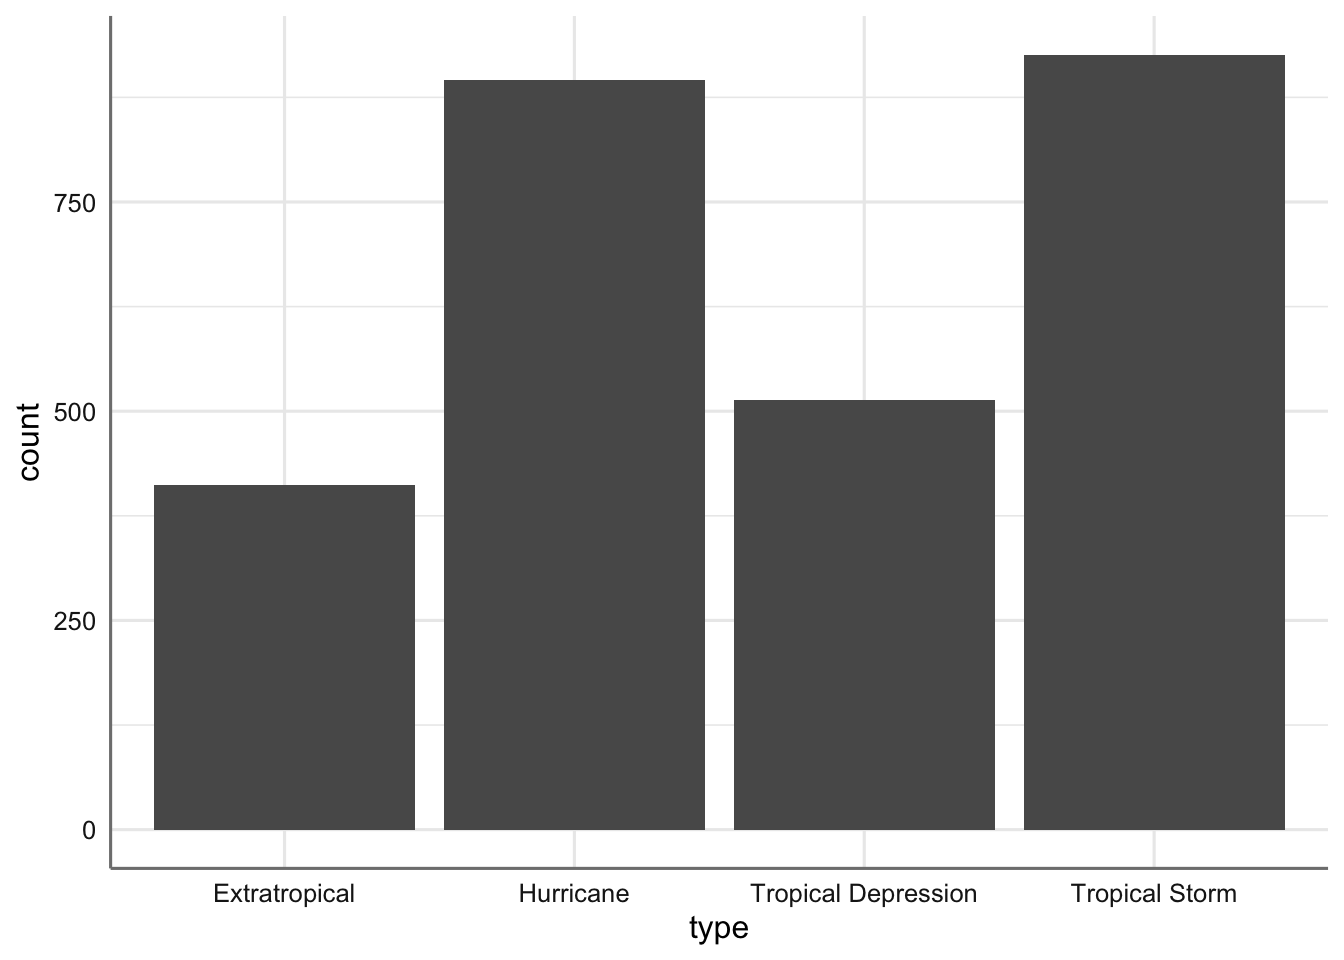
\includegraphics[width=0.95\linewidth]{02-aed_files/figure-latex/aed006-1} 

}

\caption{Gráfico de barras del tipo de tormenta.}\label{fig:aed006}
\end{figure}

Podemos personalizar este gráfico de barras si es necesario con funciones como xlab y ylab, y configurando varias propiedades dentro de geom\_bar. Por ejemplo:

\begin{Shaded}
\begin{Highlighting}[]
\CommentTok{\# Retocamos las barras para que aparezcan en azul y con un ancho inferior}
\CommentTok{\# En este caso no almacenamos el gráfico sino que lo ejecutamos directamente}
\FunctionTok{ggplot}\NormalTok{(storm, }\FunctionTok{aes}\NormalTok{(}\AttributeTok{x =}\NormalTok{ type)) }\SpecialCharTok{+} 
  \FunctionTok{geom\_bar}\NormalTok{(}\AttributeTok{fill =} \StringTok{"blue"}\NormalTok{, }\AttributeTok{width =} \FloatTok{0.7}\NormalTok{) }\SpecialCharTok{+} 
  \FunctionTok{xlab}\NormalTok{(}\StringTok{"Tipo de Tormenta"}\NormalTok{) }\SpecialCharTok{+} \FunctionTok{ylab}\NormalTok{(}\StringTok{"Número de observaciones"}\NormalTok{)}
\end{Highlighting}
\end{Shaded}

\begin{figure}

{\centering 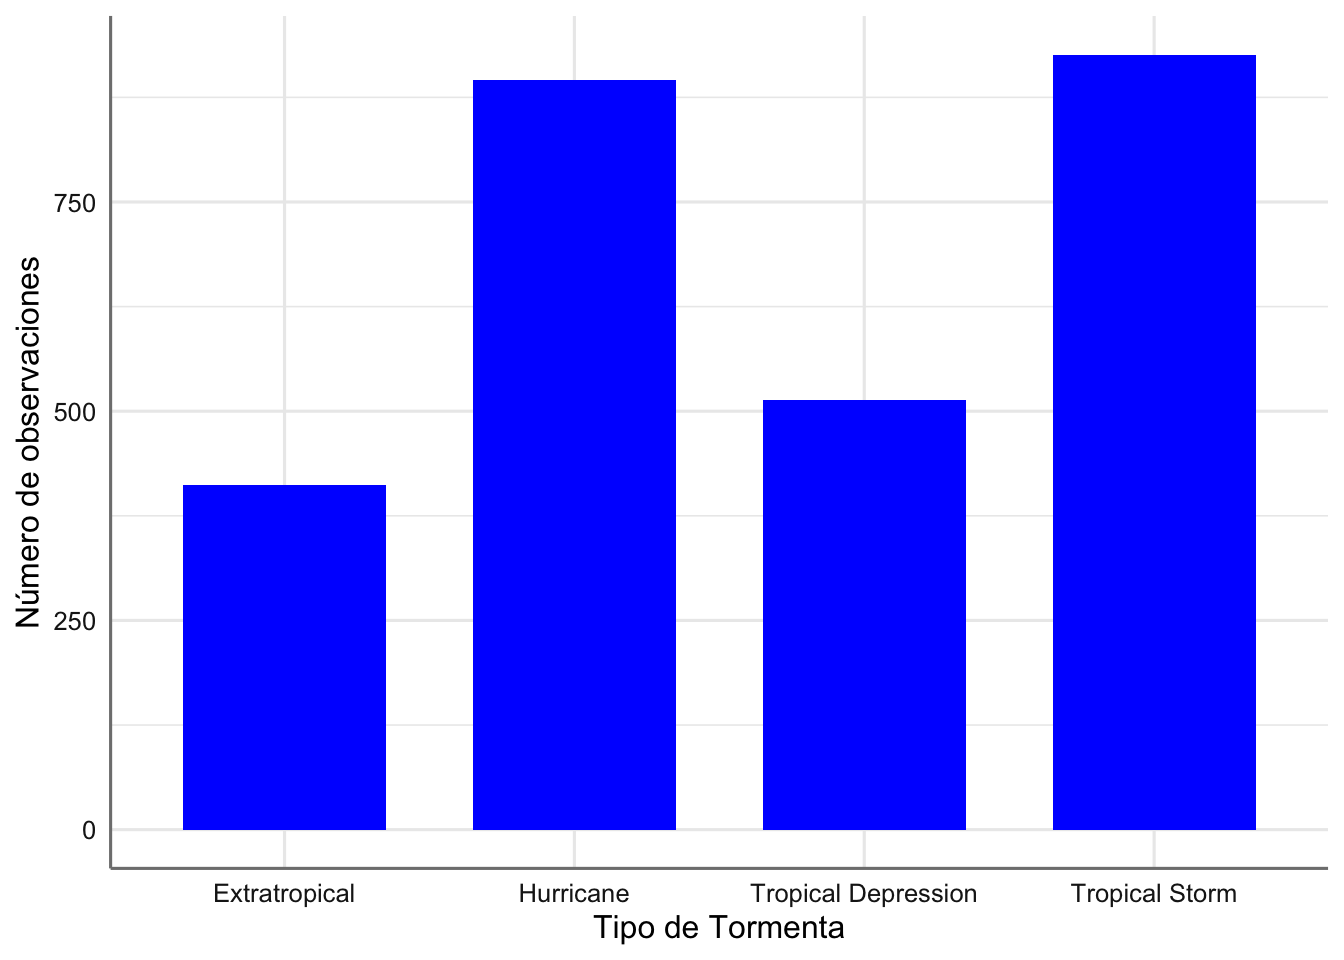
\includegraphics[width=0.95\linewidth]{02-aed_files/figure-latex/aed007-1} 

}

\caption{Gráfico de barras del tipo de tormenta (versión 2).}\label{fig:aed007}
\end{figure}

Como podemos ver tanto en las tablas obtenidas como en los dos gráficos precedentes la escala del tipo de tormenta no está ordenada, es decir, no la tenemos graduada por la relevancia de la tormenta. Veamos como podemos hacer esto e integrarlo en el gráfico:

\begin{Shaded}
\begin{Highlighting}[]
\CommentTok{\# Creamos un vector con el orden predefinido}
\NormalTok{ords }\OtherTok{\textless{}{-}} \FunctionTok{c}\NormalTok{(}\StringTok{"Tropical Depression"}\NormalTok{, }\StringTok{"Extratropical"}\NormalTok{, }\StringTok{"Tropical Storm"}\NormalTok{, }\StringTok{"Hurricane"}\NormalTok{)}
\CommentTok{\# Generamos el gráfico indica que el eje x tiene escala dada por el vector ordenado}
\FunctionTok{ggplot}\NormalTok{(storm, }\FunctionTok{aes}\NormalTok{(}\AttributeTok{x =}\NormalTok{ type)) }\SpecialCharTok{+} 
  \FunctionTok{geom\_bar}\NormalTok{(}\AttributeTok{fill =} \StringTok{"blue"}\NormalTok{, }\AttributeTok{width =} \FloatTok{0.7}\NormalTok{) }\SpecialCharTok{+} 
  \FunctionTok{scale\_x\_discrete}\NormalTok{(}\AttributeTok{limits =}\NormalTok{ ords) }\SpecialCharTok{+}
  \FunctionTok{xlab}\NormalTok{(}\StringTok{"Tipo de Tormenta"}\NormalTok{) }\SpecialCharTok{+} \FunctionTok{ylab}\NormalTok{(}\StringTok{"Número de observaciones"}\NormalTok{)}
\end{Highlighting}
\end{Shaded}

\begin{figure}

{\centering 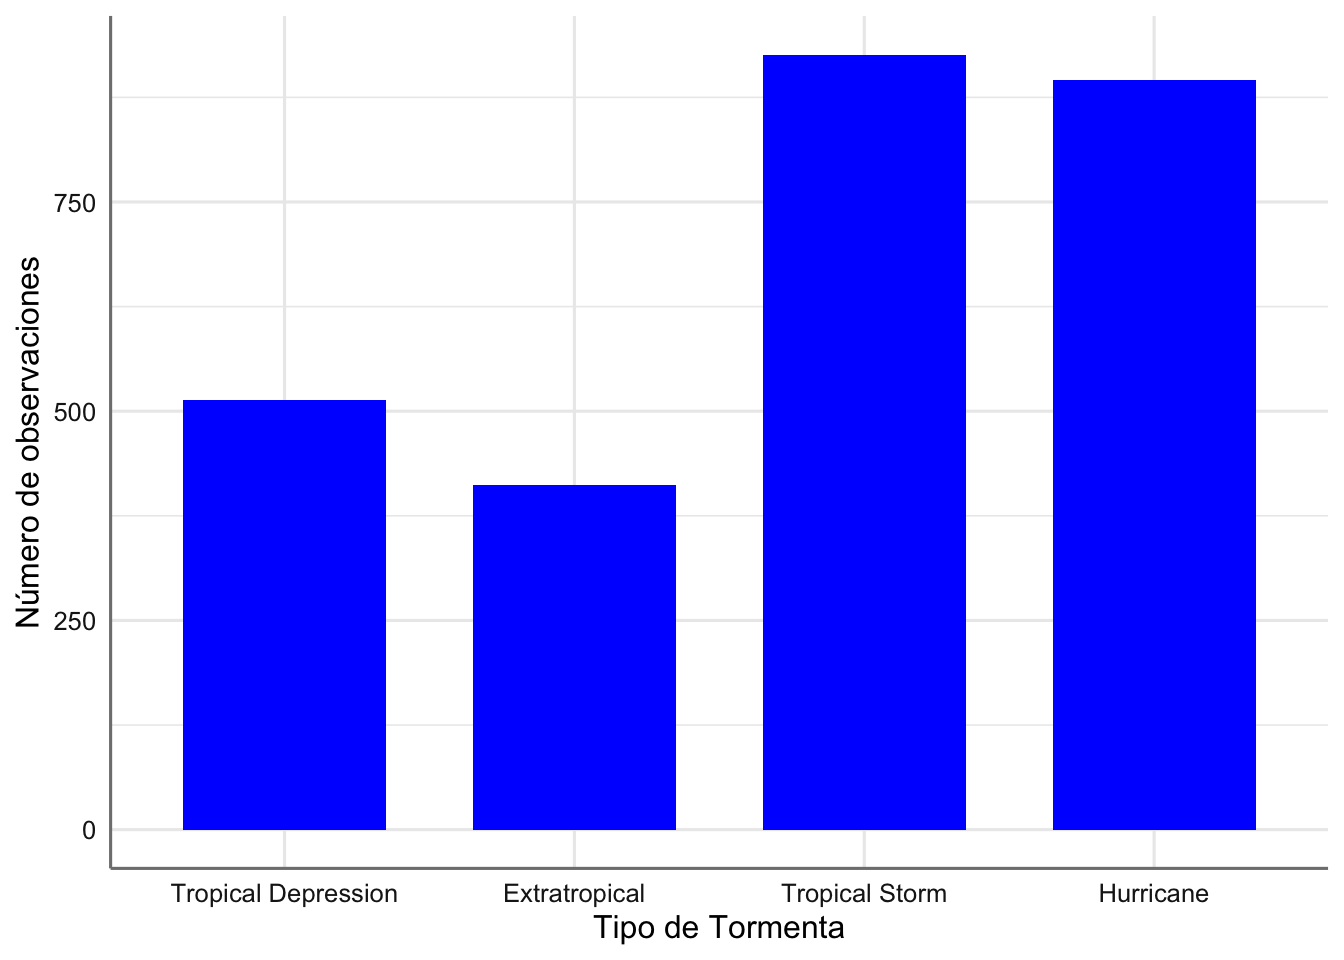
\includegraphics[width=0.95\linewidth]{02-aed_files/figure-latex/aed008-1} 

}

\caption{Gráfico de barras del tipo de tormenta (versión 3).}\label{fig:aed008}
\end{figure}

Ahora el gráfico si está ordenado con la escala adecuada y resulta más fácil cuantificar la relevancia de las tormentas más importantes. También podemos intercambiar las filas por las columnas para una mejor visualización de las etiquetas de la variable categórica. Para ello utilizamos el parámetro \texttt{coord\_flip()}:

\begin{Shaded}
\begin{Highlighting}[]
\FunctionTok{ggplot}\NormalTok{(storm, }\FunctionTok{aes}\NormalTok{(}\AttributeTok{x =}\NormalTok{ type)) }\SpecialCharTok{+} 
  \FunctionTok{geom\_bar}\NormalTok{(}\AttributeTok{fill =} \StringTok{"blue"}\NormalTok{, }\AttributeTok{width =} \FloatTok{0.7}\NormalTok{) }\SpecialCharTok{+} 
  \FunctionTok{scale\_x\_discrete}\NormalTok{(}\AttributeTok{limits =}\NormalTok{ ords) }\SpecialCharTok{+}
  \FunctionTok{coord\_flip}\NormalTok{() }\SpecialCharTok{+} 
  \FunctionTok{xlab}\NormalTok{(}\StringTok{"Tipo de Tormenta"}\NormalTok{) }\SpecialCharTok{+} \FunctionTok{ylab}\NormalTok{(}\StringTok{"Número de observaciones"}\NormalTok{)}
\end{Highlighting}
\end{Shaded}

\begin{figure}

{\centering 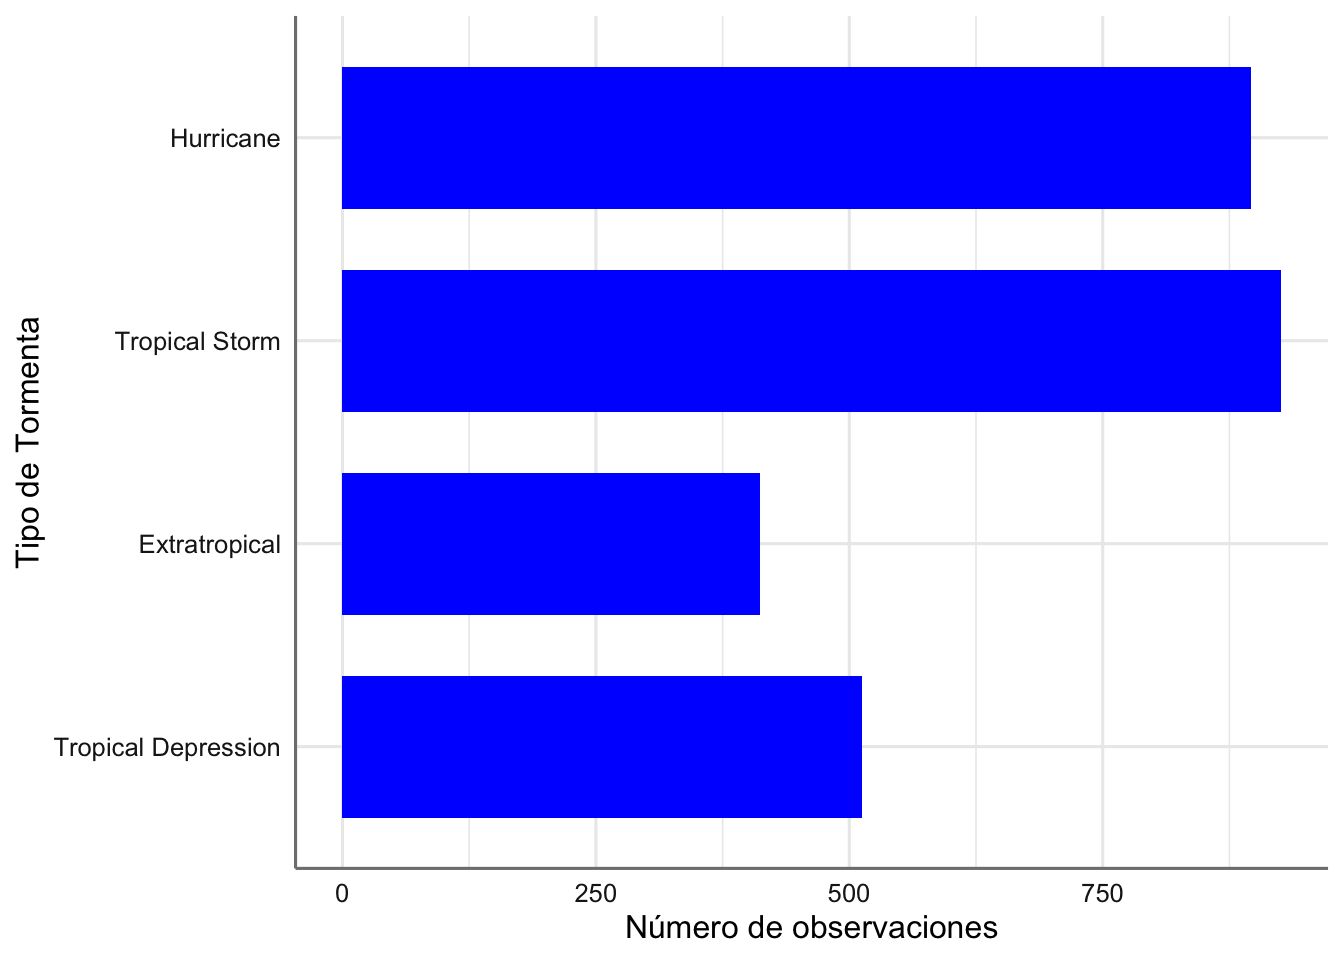
\includegraphics[width=0.95\linewidth]{02-aed_files/figure-latex/aed009-1} 

}

\caption{Gráfico de barras del tipo de tormenta (versión 4).}\label{fig:aed009}
\end{figure}

Por último utilizamos la función \texttt{theme\_bw()} para configurar un fondo blanco para el gráfico. Otras posibilidades para los temas son \texttt{theme\_classic()}, \texttt{theme\_dark()}, \texttt{theme\_grey()}, \texttt{theme\_light()}.

\begin{Shaded}
\begin{Highlighting}[]
\FunctionTok{ggplot}\NormalTok{(storm, }\FunctionTok{aes}\NormalTok{(}\AttributeTok{x =}\NormalTok{ type)) }\SpecialCharTok{+} 
  \FunctionTok{geom\_bar}\NormalTok{(}\AttributeTok{fill =} \StringTok{"blue"}\NormalTok{, }\AttributeTok{width =} \FloatTok{0.7}\NormalTok{) }\SpecialCharTok{+} 
  \FunctionTok{scale\_x\_discrete}\NormalTok{(}\AttributeTok{limits =}\NormalTok{ ords) }\SpecialCharTok{+}
  \FunctionTok{coord\_flip}\NormalTok{() }\SpecialCharTok{+} 
  \FunctionTok{xlab}\NormalTok{(}\StringTok{"Tipo de Tormenta"}\NormalTok{) }\SpecialCharTok{+} \FunctionTok{ylab}\NormalTok{(}\StringTok{"Número de observaciones"}\NormalTok{)}\SpecialCharTok{+}
  \FunctionTok{theme\_bw}\NormalTok{() }
\end{Highlighting}
\end{Shaded}

\begin{figure}

{\centering 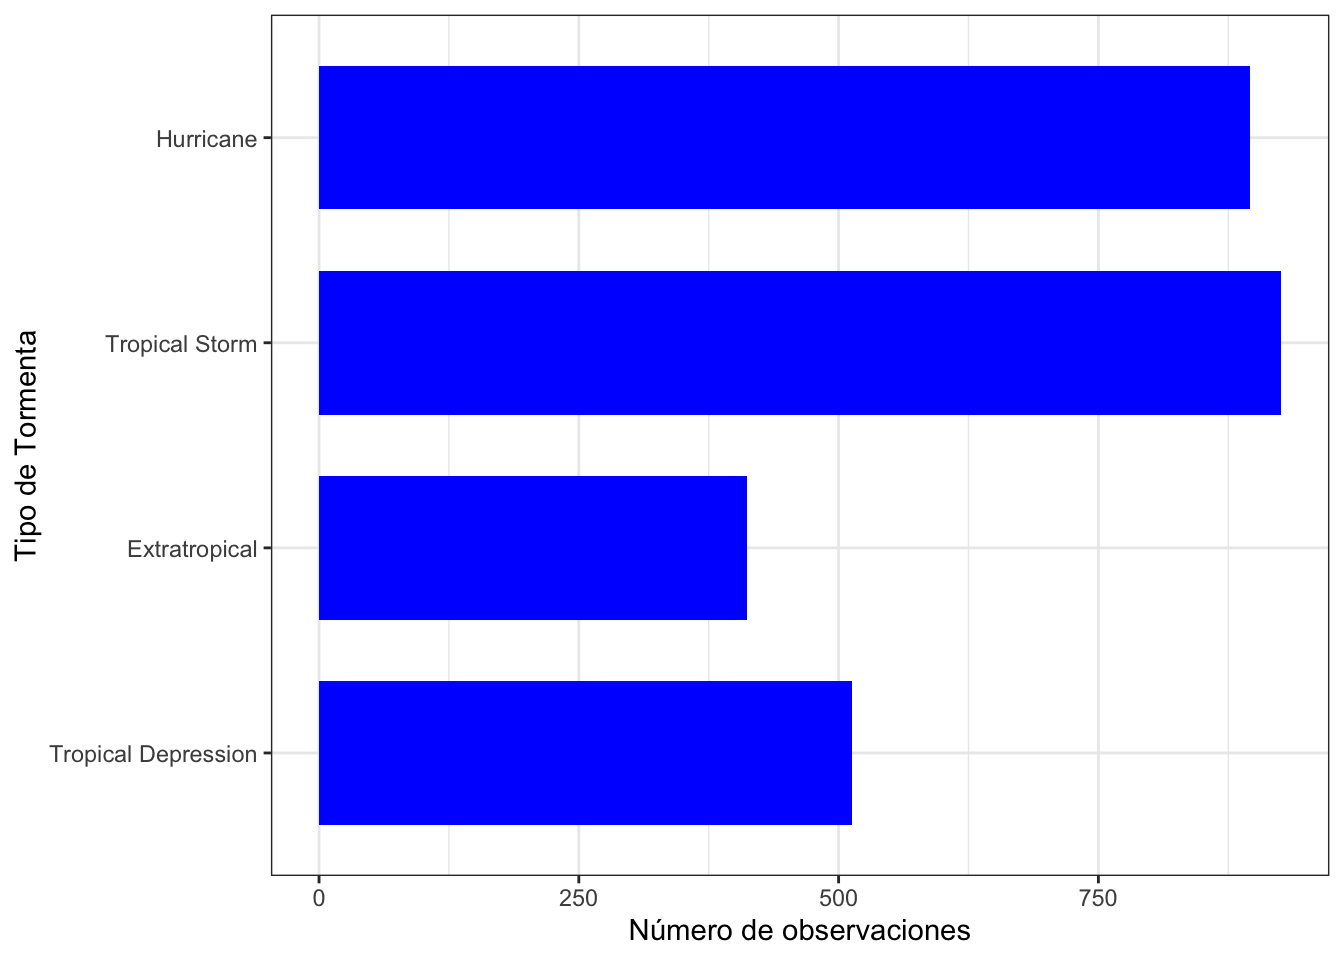
\includegraphics[width=0.95\linewidth]{02-aed_files/figure-latex/aed010-1} 

}

\caption{Gráfico de barras del tipo de tormenta (versión 5).}\label{fig:aed010}
\end{figure}

En lugar de representar los contesos podemos visualizar los porcentajes asociados a cada categoría en lugar de los conteos haciendo uso de la variable \texttt{..prop..} en la configuración de \texttt{geom\_bar()}. Se debe modificar la escala de la varaible para indicar que estamos representando porcentajes (\texttt{labels\ =\ scales::percent}):

\begin{Shaded}
\begin{Highlighting}[]
\FunctionTok{ggplot}\NormalTok{(storm, }\FunctionTok{aes}\NormalTok{(}\AttributeTok{x =}\NormalTok{ type)) }\SpecialCharTok{+} 
  \FunctionTok{geom\_bar}\NormalTok{(}\FunctionTok{aes}\NormalTok{(}\AttributeTok{y =}\NormalTok{ ..prop.. , }\AttributeTok{group =} \DecValTok{1}\NormalTok{),}\AttributeTok{fill =} \StringTok{"blue"}\NormalTok{, }\AttributeTok{width =} \FloatTok{0.7}\NormalTok{) }\SpecialCharTok{+} 
  \FunctionTok{scale\_y\_continuous}\NormalTok{(}\AttributeTok{labels =}\NormalTok{ scales}\SpecialCharTok{::}\NormalTok{percent) }\SpecialCharTok{+}
  \FunctionTok{coord\_flip}\NormalTok{() }\SpecialCharTok{+} 
  \FunctionTok{xlab}\NormalTok{(}\StringTok{"Tipo de Tormenta"}\NormalTok{) }\SpecialCharTok{+} \FunctionTok{ylab}\NormalTok{(}\StringTok{"Porcentaje"}\NormalTok{)}\SpecialCharTok{+}
  \FunctionTok{theme\_bw}\NormalTok{() }
\end{Highlighting}
\end{Shaded}

\begin{figure}

{\centering 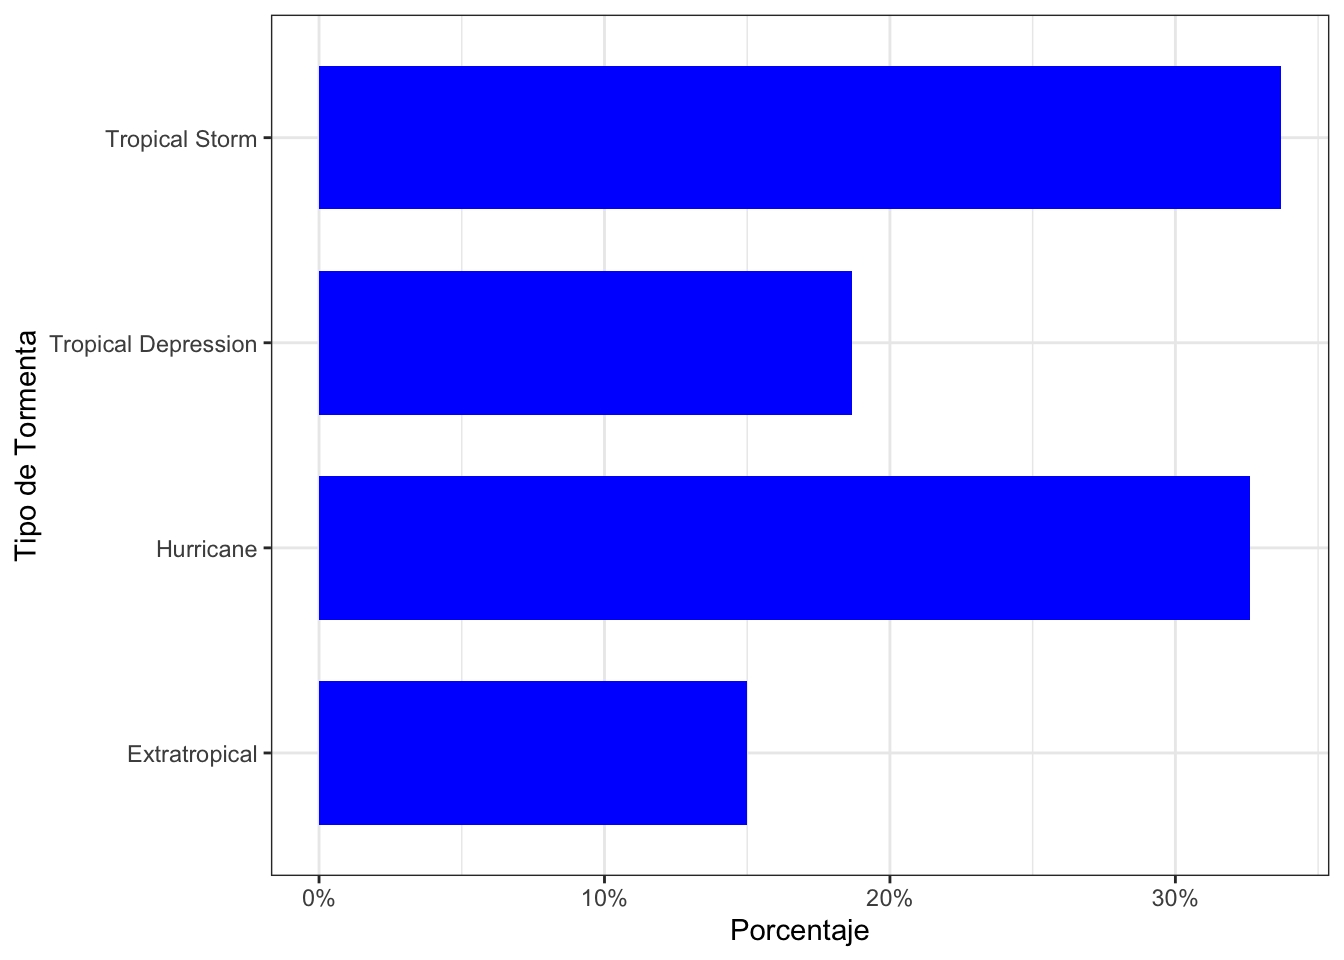
\includegraphics[width=0.95\linewidth]{02-aed_files/figure-latex/aed011-1} 

}

\caption{Gráfico de barras del porcentaje de cada tipo de tormenta.}\label{fig:aed011}
\end{figure}

\hypertarget{una-variable-numuxe9rica}{%
\subsection{Una variable numérica}\label{una-variable-numuxe9rica}}

En esta sección se considera cómo explorar la distribución de una variable numérica Se presentan las descriptivas básicas y visualizaciones que son apropiadas para las variables de este tipo. Para ejemplificar los procedimientos utilizaremos las variables \texttt{wind} y \texttt{pressure}.

\hypertarget{resuxfamenes-numuxe9ricos-1}{%
\subsubsection{Resúmenes numéricos}\label{resuxfamenes-numuxe9ricos-1}}

Hasta ahora hemos estado describiendo las propiedades de las distribuciones de muestra en términos muy generales, usando frases como ``valores más comunes'' y ``el rango de los datos'' sin decir realmente lo que queremos decir. Los estadísticos han ideado términos específicos para describir este tipo de propiedades, así como diferentes estadísticas descriptivas para cuantificarlas. Los dos que más importan son la tendencia central y la dispersión:

\begin{itemize}
\tightlist
\item
  Una \textbf{medida de tendencia central} describe un valor típico (`central') de una distribución de datos. La medida de localización más extendida es la media aritmética de una muestra. Hay muchas medidas diferentes de tendencia central, cada una con sus propios pros y contras. Entre estos, la mediana es la que se usa con mayor frecuencia en los análisis exploratorios ya que es le valor que nos divide la muestra de dos partes iguales situando el 50\% de los datos a cada lado de ese valor.
\item
  Una \textbf{medida de dispersión} describe cómo se distribuye una distribución. Las medidas de dispersión cuantifican la variabilidad o dispersión de una variable con respecto al promedio de los datos. Si una distribución está más dispersa que otra, significa que, en cierto sentido, abarca una gama más amplia de valores. Lo que esto significa en la práctica depende del tipo de medida con la que estamos trabajando. Las medidas de dispersión más habituales son la varianza y su raíz cuadrada, la desviación estándar.
\end{itemize}

\hypertarget{medidas-de-tendencia-central}{%
\paragraph{Medidas de tendencia central}\label{medidas-de-tendencia-central}}

Hay dos estadísticos que se utilizan generalmente para describir la tendencia central de la distribución de los datos muestrales de un variable numérica. De ahora en adelante denotamos por \(n\) al tamaño muestral y \(x_1, x_2,...,x_n\) los valores muestrales de la variable que deseamos estudiar.

La media muestral es la medida de tendencia muestral por excelencia. La definición matemática de la media muestral viene dada por: \begin{equation} 
  \bar{x} = \frac{\sum_{i=1}^n x_i}{n}
  \label{eq:samplemean}
\end{equation}

Para obtener la media utilizamos la función \texttt{mean()}

\begin{Shaded}
\begin{Highlighting}[]
\FunctionTok{mean}\NormalTok{(storm}\SpecialCharTok{$}\NormalTok{wind)}
\end{Highlighting}
\end{Shaded}

\begin{verbatim}
## [1] 54.68329
\end{verbatim}

\begin{Shaded}
\begin{Highlighting}[]
\FunctionTok{mean}\NormalTok{(storm}\SpecialCharTok{$}\NormalTok{pressure)}
\end{Highlighting}
\end{Shaded}

\begin{verbatim}
## [1] 989.8238
\end{verbatim}

Esto nos dice que la media de la velocidad del viento es de 55 mph y que la media de la presión es de 989.82 milibares. ¿Como podemos interpretar esos resultados?

Una limitación de la media aritmética es que se ve afectada por la forma de la distribución de los datos. Es muy sensible a los extremos de una muestra. Esta es la razón por la cual, por ejemplo, no tiene mucho sentido mirar el ingreso medio de los trabajadores en un país para tener una idea de lo que gana una persona ``típica''. La distribución del ingreso es muy asimétrica, y los pocos que tienen la suerte de ganar salarios muy buenos tienden a cambiar la media hacia arriba y superar cualquier cosa que sea realmente ``típica''. La media de la muestra también se ve fuertemente afectada por la presencia de `valores atípicos' o valores extremos, es decir, valores inusualmente grandes o pequeños en una muestra.

Debido a que la media muestral es sensible a la forma de una distribución y la presencia de valores atípicos, a menudo se prefiere una segunda medida de tendencia central: la mediana de la muestra. La mediana de una muestra es el número que separa los datos en dos subgrupos (la mitad superior de la mitad inferior). Podemos calcular la mediana muestral en R con la función \texttt{median()}:

\begin{Shaded}
\begin{Highlighting}[]
\FunctionTok{median}\NormalTok{(storm}\SpecialCharTok{$}\NormalTok{wind)}
\end{Highlighting}
\end{Shaded}

\begin{verbatim}
## [1] 50
\end{verbatim}

\begin{Shaded}
\begin{Highlighting}[]
\FunctionTok{median}\NormalTok{(storm}\SpecialCharTok{$}\NormalTok{pressure)}
\end{Highlighting}
\end{Shaded}

\begin{verbatim}
## [1] 995
\end{verbatim}

Estos resultados indican que el 50\% de de los registros muestran una valor de viento inferior a 50 mph. De la misma forma el 50\% de los datos muestran una valor de la presión inferior a 995 milibares.

Otras medidas de localización son el mínimo, el máximo y los percentiles. Los percentiles son los valores que dividen en la muestra según el valor del percentil solicitado. Si solicitamos el percentil 20, se separa la muestra en dos subconjuntos dejando el 20\% en un grupo y e 80\% en el otro. Los percentiles más habituales son lo denominados primer y tercer cuartil que corresponden a los percentiles 25 y 75 respectivamente. Para obtener el percentil asociado a una variable numérica podemos hacer uso de la función \texttt{quantile()}. Para ver como se debe utilizar es útil consultar la ayuda de dicha función \texttt{help(quantile)}.

\hypertarget{medidas-de-dispersiuxf3n}{%
\paragraph{Medidas de dispersión}\label{medidas-de-dispersiuxf3n}}

Hay muchas maneras de cuantificar la dispersión de un conjunto de datos muestrales de una variable numérica. Los valores más importantes desde el punto de vista estadístico son la varianza muestral y la desviación estándar. La varianza muestral \(s^2\) es ``la suma de las desviaciones cuadradas'' (es decir, las diferencias) de cada observación con respecto a la media de la muestra, dividida por el tamaño de la muestra menos uno. La desviación típica es la raíz cuadrada de la varianza muestral. Las definiciones matemáticas de ambas cantidades son: \begin{equation} 
  s^2 = \frac{\sum_{i=1}^n (x_i-\bar{x})^2}{n-1}
  \label{eq:var}
\end{equation}

\begin{equation} 
  s = \sqrt{s^2}
  \label{eq:sd}
\end{equation}

Las funciones de R para calcular ambas cantidades son \texttt{var()} para la varianza y \texttt{sd()} para la desviación típica.

\begin{Shaded}
\begin{Highlighting}[]
\FunctionTok{var}\NormalTok{(storm}\SpecialCharTok{$}\NormalTok{wind);}\FunctionTok{sd}\NormalTok{(storms}\SpecialCharTok{$}\NormalTok{wind)}
\end{Highlighting}
\end{Shaded}

\begin{verbatim}
## [1] 668.1444
\end{verbatim}

\begin{verbatim}
## [1] 25.84849
\end{verbatim}

\begin{Shaded}
\begin{Highlighting}[]
\FunctionTok{var}\NormalTok{(storm}\SpecialCharTok{$}\NormalTok{pressure);}\FunctionTok{sd}\NormalTok{(storms}\SpecialCharTok{$}\NormalTok{pressure)}
\end{Highlighting}
\end{Shaded}

\begin{verbatim}
## [1] 349.4912
\end{verbatim}

\begin{verbatim}
## [1] 18.69468
\end{verbatim}

¿Qué significa ese número en realidad? Las variaciones son siempre no negativas. Una pequeña varianza indica que las observaciones tienden a ser cercanas a la media (y una a la otra), mientras que una alta varianza indica que las observaciones están muy dispersas. Una varianza de cero solo ocurre si todos los valores son idénticos. Sin embargo, es difícil interpretar si una varianza muestral es realmente ``pequeña'' o ``grande'' porque el cálculo involucra desviaciones al cuadrado. Por ejemplo, cambiar la escala de medición de una variable por 10 implica un cambio de 100 veces (102) en la varianza.

La varianza es una cantidad importante en las estadísticas que aparece una y otra vez. Muchas herramientas estadísticas comunes usan cambios en la varianza para comparar formalmente qué tan bien diferentes modelos describen un conjunto de datos. Sin embargo, es muy difícil interpretar las variaciones, por lo que rara vez las utilizamos en el trabajo exploratorio. Para expresar la variabilidad en la misma escala de la variable original utilizamos la desviación típica. En este caso se puede observar una mayor variabilidad en la variable presión atmosférica (desviación típica de 25.84 milibares) que en la variable de viento (18.69 mph).

La desviación estándar de la muestra no está exenta de problemas. Al igual que la media muestral, es sensible a la forma de la distribución de los datos y a la presencia de valores atípicos. Una medida de dispersión más robusta para este tipo de características es el rango intercuartílico, definida como la diferencia entre el percentil 75 (tercer cuartil) y el percentil 25 (primer cuartil):

\begin{equation} 
 IQR = Q_3 - Q_1
  \label{eq:iqr}
\end{equation}

Obviamente, cuanto más dispersos estén los datos, mayor será el IQR. La razón por la que preferimos usar IQR para medir la dispersión es que solo depende de los datos en el ``medio'' de una distribución de muestra. Esto lo hace robusto a la presencia de valores atípicos. Podemos usar la función \texttt{IQR()} para calcular el rango intercuartílico:

\begin{Shaded}
\begin{Highlighting}[]
\FunctionTok{IQR}\NormalTok{(storm}\SpecialCharTok{$}\NormalTok{wind)}
\end{Highlighting}
\end{Shaded}

\begin{verbatim}
## [1] 35
\end{verbatim}

\begin{Shaded}
\begin{Highlighting}[]
\FunctionTok{IQR}\NormalTok{(storm}\SpecialCharTok{$}\NormalTok{pressure)}
\end{Highlighting}
\end{Shaded}

\begin{verbatim}
## [1] 24
\end{verbatim}

La última medidad de dispersión que veremos es el coeficiente de variación. Esta medida es una de las más habituales y se obtiene a partir de la media y desviación típica muestral como: \begin{equation} 
 CV = \frac{s}{\bar{x}}
  \label{eq:cv}
\end{equation}

Su fórmula expresa la desviación estándar como porcentaje de la media aritmética, mostrando una interpretación relativa del grado de variabilidad, independiente de la escala de la variable, a diferencia de la desviación típica o estándar. De esta forma, valores bajos del coeficiente de variación expresan menor variabilidad, lo que resulta de utilidad cuando deseamos comparar la variabilidad de dos muestras independeintemente de su media. El mayor problema es que sólo puede ser usado cuando la media muestral es positiva.

\hypertarget{resuxfamenes-conjuntos}{%
\paragraph{Resúmenes conjuntos}\label{resuxfamenes-conjuntos}}

Aunque podemos ir calculando cada una de las medidas de localización y dispersión vistas anteriormente, en la práctica nos resulta más útil obtenerlas todas de una vez. Existen diferentes funciones que nos permiten obterner estos análisis descriptivos. La primera de ellas es la función \texttt{summary()} que nos porporciona el mínimo, máximo, media, mediana y los percentiles 25 y 75. Sin embargo, no nos porporciona ninguna de las medidas de varaibilidad usuales. En nuestro ejemplo

\begin{Shaded}
\begin{Highlighting}[]
\FunctionTok{summary}\NormalTok{(storm}\SpecialCharTok{$}\NormalTok{wind)}
\end{Highlighting}
\end{Shaded}

\begin{verbatim}
##    Min. 1st Qu.  Median    Mean 3rd Qu.    Max. 
##   15.00   35.00   50.00   54.68   70.00  155.00
\end{verbatim}

\begin{Shaded}
\begin{Highlighting}[]
\FunctionTok{summary}\NormalTok{(storm}\SpecialCharTok{$}\NormalTok{pressure)}
\end{Highlighting}
\end{Shaded}

\begin{verbatim}
##    Min. 1st Qu.  Median    Mean 3rd Qu.    Max. 
##   905.0   980.0   995.0   989.8  1004.0  1019.0
\end{verbatim}

Se pude ver que el 25\% de las observaciones muestran una valor de viento inferior a 35mph y un 25\% un valor de viento superior a 70mph. Con respecto a la presión atmosférica tenemos que el 25\% de las observaciones tienen un valor inferior a 980 milibares, y un 25\% tienen un valor superior a 1004 milibares.

Otra función que nos porporciona medidas conjuntas es \texttt{estat()} de la librería \texttt{pubh}. Esta función nos porporciona el número de casos, el mínimo, el máximo, la media, la mediana, la desviación típica, y el coeficiente de variación.

\begin{Shaded}
\begin{Highlighting}[]
\CommentTok{\# Etiquetamos las variables}
\NormalTok{storm }\OtherTok{=}\NormalTok{ storm }\SpecialCharTok{\%\textgreater{}\%} 
  \FunctionTok{var\_labels}\NormalTok{(}\AttributeTok{wind =} \StringTok{\textquotesingle{}Wind speed (in knots)\textquotesingle{}}\NormalTok{, }
             \AttributeTok{pressure =} \StringTok{\textquotesingle{}Air pressure (in mbar)\textquotesingle{}}\NormalTok{)}
\CommentTok{\# Análisis descriptivos}
\FunctionTok{estat}\NormalTok{(}\SpecialCharTok{\textasciitilde{}}\NormalTok{ wind, }\AttributeTok{data =}\NormalTok{ storm)}
\end{Highlighting}
\end{Shaded}

\begin{verbatim}
##                            N Min. Max.  Mean Median    SD   CV
## 1 Wind speed (in knots) 2747   15  155 54.68     50 25.85 0.47
\end{verbatim}

\begin{Shaded}
\begin{Highlighting}[]
\FunctionTok{estat}\NormalTok{(}\SpecialCharTok{\textasciitilde{}}\NormalTok{ pressure, }\AttributeTok{data =}\NormalTok{ storm)}
\end{Highlighting}
\end{Shaded}

\begin{verbatim}
##                             N Min. Max.   Mean Median    SD   CV
## 1 Air pressure (in mbar) 2747  905 1019 989.82    995 18.69 0.02
\end{verbatim}

\hypertarget{visualizaciuxf3n-gruxe1fica-1}{%
\subsubsection{Visualización gráfica}\label{visualizaciuxf3n-gruxe1fica-1}}

En este apartado veremos como representar los datos de los conteos de una variable categórica mediante la función 'ggplot`. Esta función permite realizar casi cualquier tipo de gráfico que podamos imaginar. En este punto vamos a ir presentando diferentes parámetros de dicha función para ir familiarizándonos con su uso.

\hypertarget{gruxe1fico-barras-1}{%
\paragraph{Gráfico barras}\label{gruxe1fico-barras-1}}

El gráfico por excelencia para una variable de tipo numérico es el denominado histograma. El histograma es una representación mediante barras de la distribución de los datos. Para construir las barras se divide el rango de la variable numérica en un conjunto fijo de intervalos disjuntos y se contabiliza el número de datos que quedan dentro de cada uno de ellos (altura del gráfico de barras). Es un gráfico muy interesante porque representa de forma bastante precisa, ajustando el número de intervalos, la distribución del conjunto de datos pudiéndose observar su dispersión y/o asimetria.

Para realizar este gráfico utilizamos parámetros específicos dentro de la función \texttt{ggplot()} a partir de \texttt{geom\_histogram()}.

\begin{Shaded}
\begin{Highlighting}[]
\FunctionTok{ggplot}\NormalTok{(storm, }\FunctionTok{aes}\NormalTok{(}\AttributeTok{x =}\NormalTok{ pressure)) }\SpecialCharTok{+}
   \FunctionTok{geom\_histogram}\NormalTok{()}
\end{Highlighting}
\end{Shaded}

\begin{figure}

{\centering 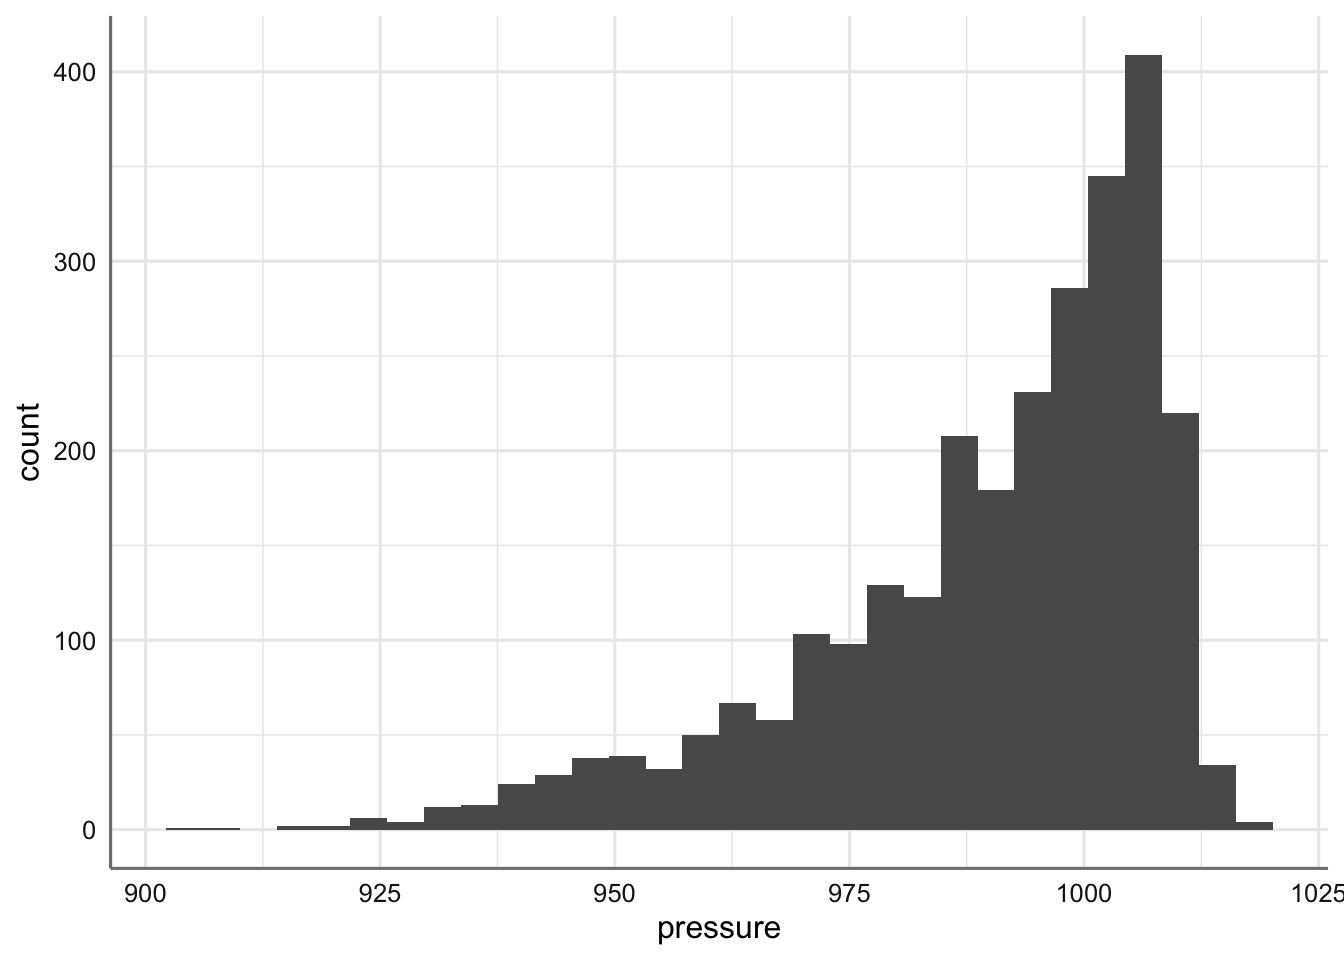
\includegraphics[width=0.95\linewidth]{02-aed_files/figure-latex/aed018-1} 

}

\caption{Histograma de la presión atmosférica.}\label{fig:aed018}
\end{figure}

Podemos ver que la mayoría de los datos se sitúan por encima de 915 milibares, hay una clara asimetría hacia los valores más grandes y existe una gran dispersión entre en el conjunto de valores observados.

Veamos como introducir diferentes parámetros en el gráfico anterior. el más importante es el que hace referencia a los intervalos asociado con el histograma (parámetro \texttt{binwith})

\begin{Shaded}
\begin{Highlighting}[]
\FunctionTok{ggplot}\NormalTok{(storm, }\FunctionTok{aes}\NormalTok{(}\AttributeTok{x =}\NormalTok{ pressure)) }\SpecialCharTok{+} 
  \FunctionTok{geom\_histogram}\NormalTok{(}\AttributeTok{binwidth =} \DecValTok{8}\NormalTok{, }\AttributeTok{fill =} \StringTok{"steelblue"}\NormalTok{) }\SpecialCharTok{+} 
  \FunctionTok{xlab}\NormalTok{(}\StringTok{"Air pressure (in mbar)"}\NormalTok{) }\SpecialCharTok{+} \FunctionTok{ylab}\NormalTok{(}\StringTok{"Frequency"}\NormalTok{)}
\end{Highlighting}
\end{Shaded}

\begin{figure}

{\centering 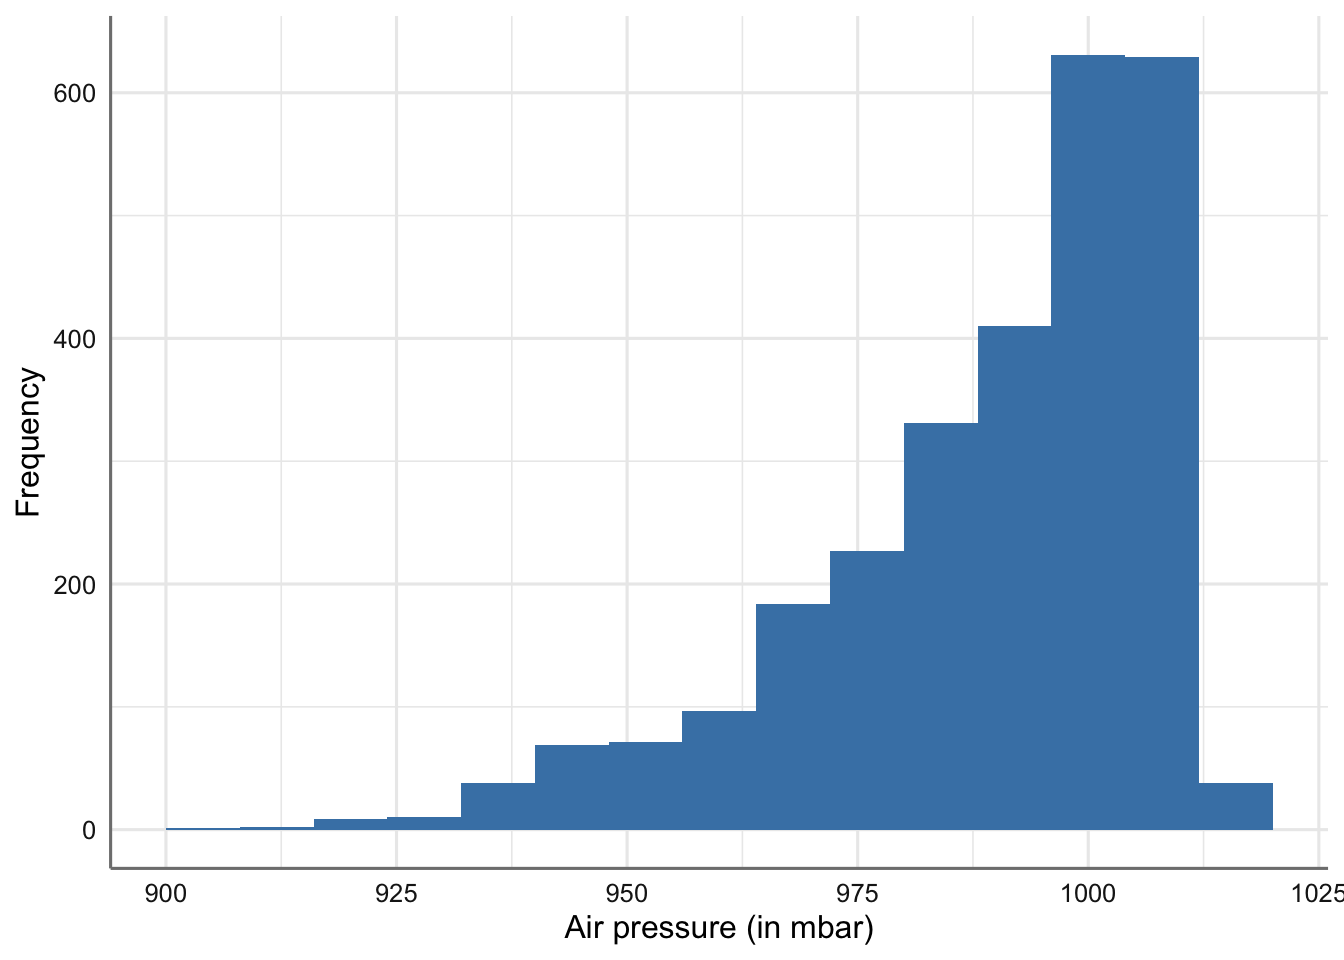
\includegraphics[width=0.95\linewidth]{02-aed_files/figure-latex/aed019-1} 

}

\caption{Histograma de la presión atmosférica (modificando binwidth).}\label{fig:aed019}
\end{figure}

Veamos ahora el histograma de la variable \texttt{wind}

\begin{Shaded}
\begin{Highlighting}[]
\FunctionTok{ggplot}\NormalTok{(storm, }\FunctionTok{aes}\NormalTok{(}\AttributeTok{x =}\NormalTok{ wind)) }\SpecialCharTok{+} 
  \FunctionTok{geom\_histogram}\NormalTok{(}\AttributeTok{binwidth =} \DecValTok{8}\NormalTok{, }\AttributeTok{fill =} \StringTok{"steelblue"}\NormalTok{) }\SpecialCharTok{+} 
  \FunctionTok{xlab}\NormalTok{(}\StringTok{"Wind speed (in knots)"}\NormalTok{) }\SpecialCharTok{+} \FunctionTok{ylab}\NormalTok{(}\StringTok{"Frequency"}\NormalTok{)}
\end{Highlighting}
\end{Shaded}

\begin{figure}

{\centering 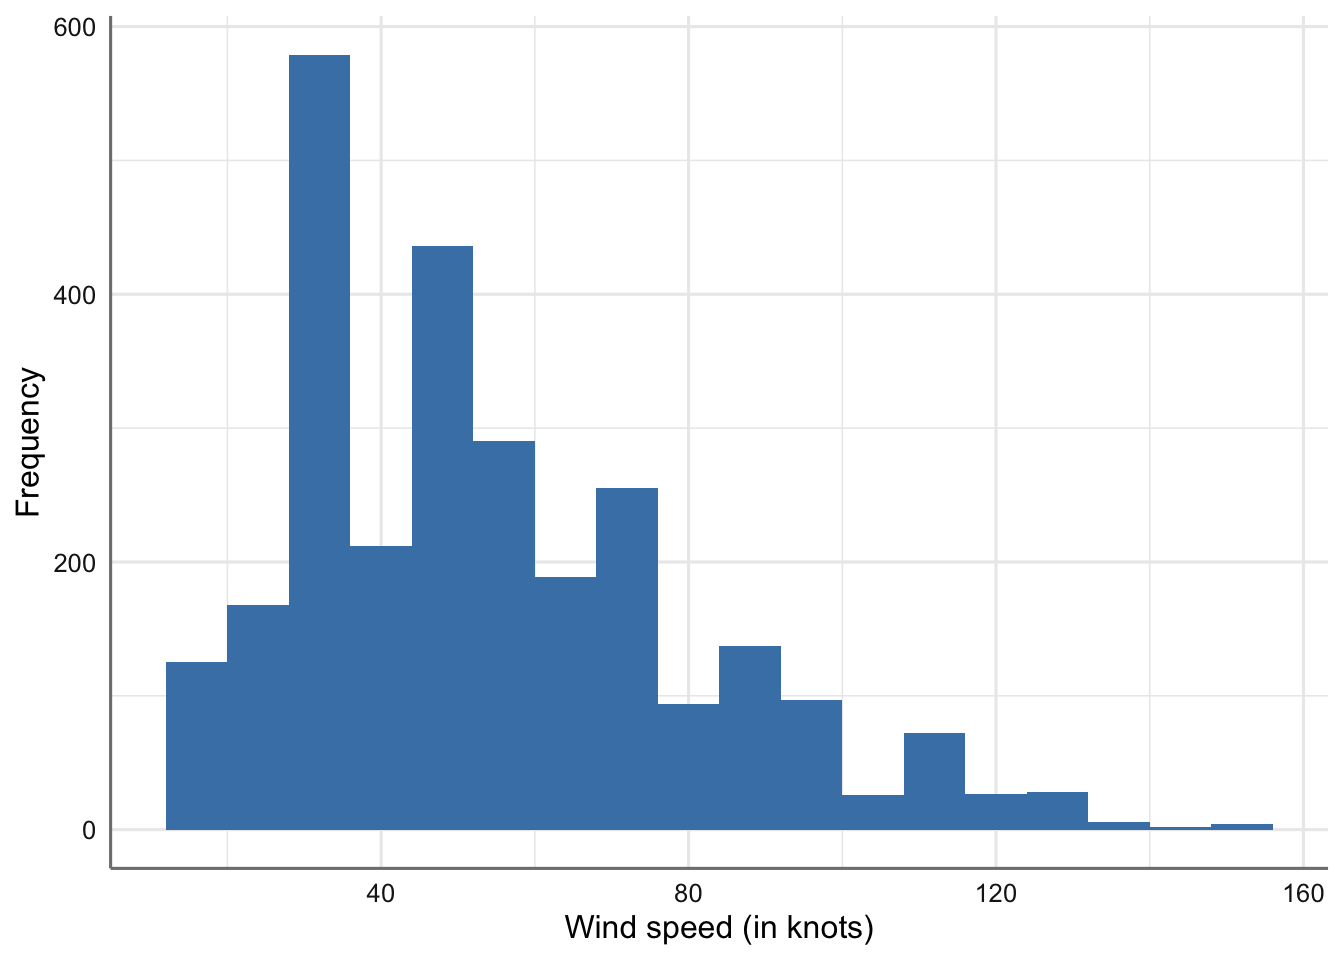
\includegraphics[width=0.95\linewidth]{02-aed_files/figure-latex/aed020-1} 

}

\caption{Histograma de la velocidad del viento.}\label{fig:aed020}
\end{figure}

El otro gráfico habitual para una variable de tipo numérico es el llamado gráfico de cajas. En este gráfico se representa mediante una caja la media (linea central de la caja), el percentil 75 (línea superior de la caja), y el percentil 25 (linea inferior de la caja). También se representan el valor máximo (percentil 75 + 1.5 IQR) y mínimo (percentil 25 - 1.5 IQR), así como los caracterizados como valores extremos (punto fuera de la caja). Veamos como realizar este gráfico mediante el parámetro \texttt{geom\_boxplot()}.

\begin{Shaded}
\begin{Highlighting}[]
\FunctionTok{ggplot}\NormalTok{(storm, }\FunctionTok{aes}\NormalTok{(}\AttributeTok{x =} \FunctionTok{factor}\NormalTok{(}\DecValTok{1}\NormalTok{),}\AttributeTok{y =}\NormalTok{ pressure)) }\SpecialCharTok{+}
   \FunctionTok{geom\_boxplot}\NormalTok{()}
\end{Highlighting}
\end{Shaded}

\begin{figure}

{\centering 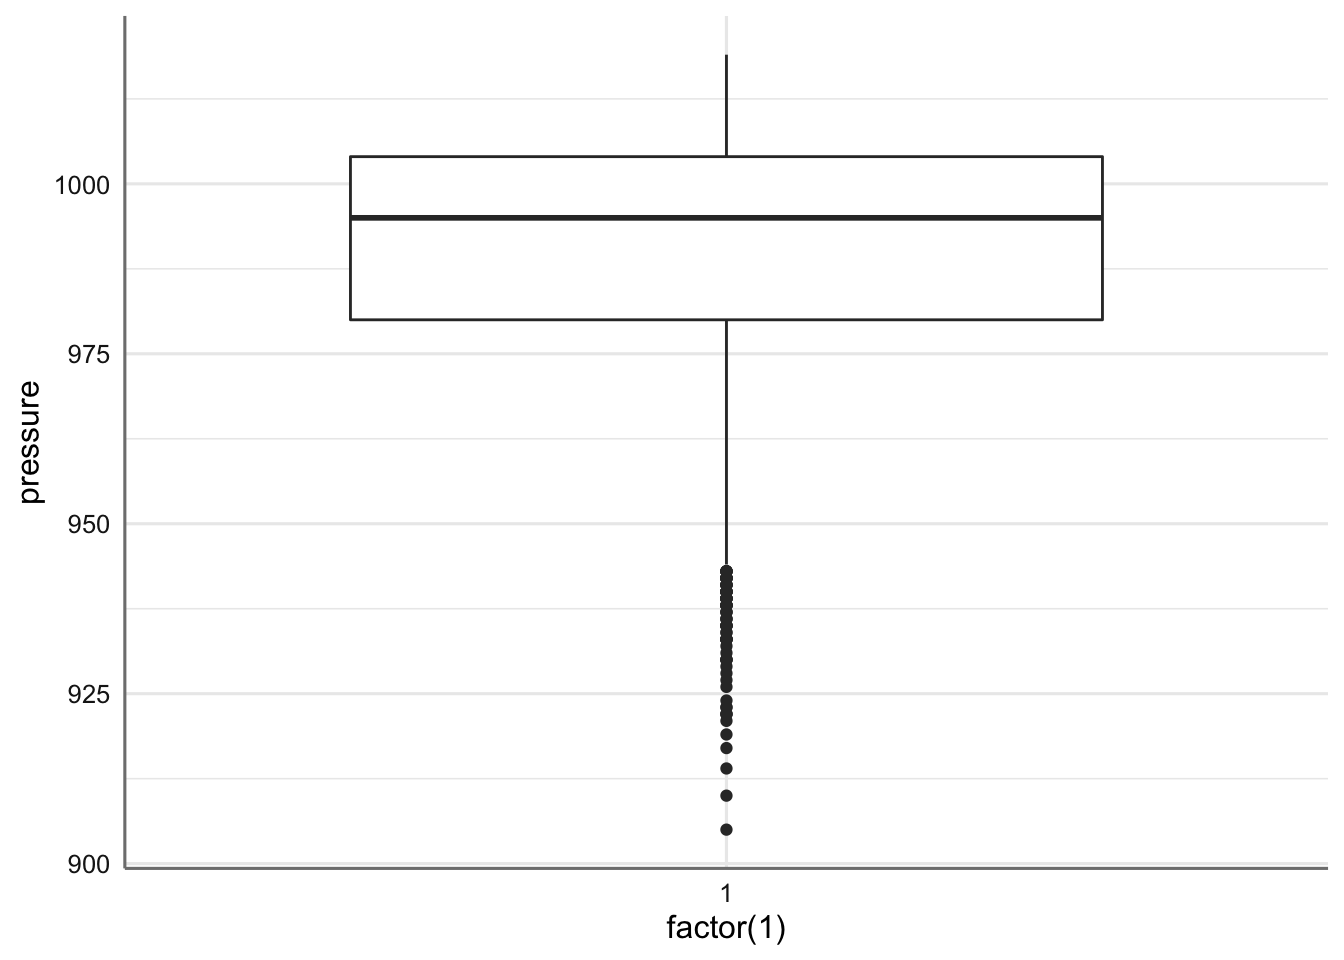
\includegraphics[width=0.95\linewidth]{02-aed_files/figure-latex/aed021-1} 

}

\caption{Gráfico de cajas de la presión atmosférica.}\label{fig:aed021}
\end{figure}

Añadimos parámetros (título de ejes, color caja, selección de valores extremos, y fondo blanco)

\begin{Shaded}
\begin{Highlighting}[]
\FunctionTok{ggplot}\NormalTok{(storm, }\FunctionTok{aes}\NormalTok{(}\AttributeTok{x =} \FunctionTok{factor}\NormalTok{(}\DecValTok{1}\NormalTok{), }\AttributeTok{y =}\NormalTok{ pressure)) }\SpecialCharTok{+}
   \FunctionTok{geom\_boxplot}\NormalTok{(}\AttributeTok{fill =} \StringTok{"orange"}\NormalTok{, }\AttributeTok{outlier.colour =} \StringTok{"red"}\NormalTok{, }\AttributeTok{outlier.shape =} \DecValTok{1}\NormalTok{) }\SpecialCharTok{+}
   \FunctionTok{scale\_x\_discrete}\NormalTok{(}\AttributeTok{name =} \StringTok{" "}\NormalTok{) }\SpecialCharTok{+} \FunctionTok{scale\_y\_continuous}\NormalTok{(}\AttributeTok{name =} \StringTok{"Air pressure (in mbar)"}\NormalTok{) }\SpecialCharTok{+}
   \FunctionTok{theme\_bw}\NormalTok{()}
\end{Highlighting}
\end{Shaded}

\begin{figure}

{\centering 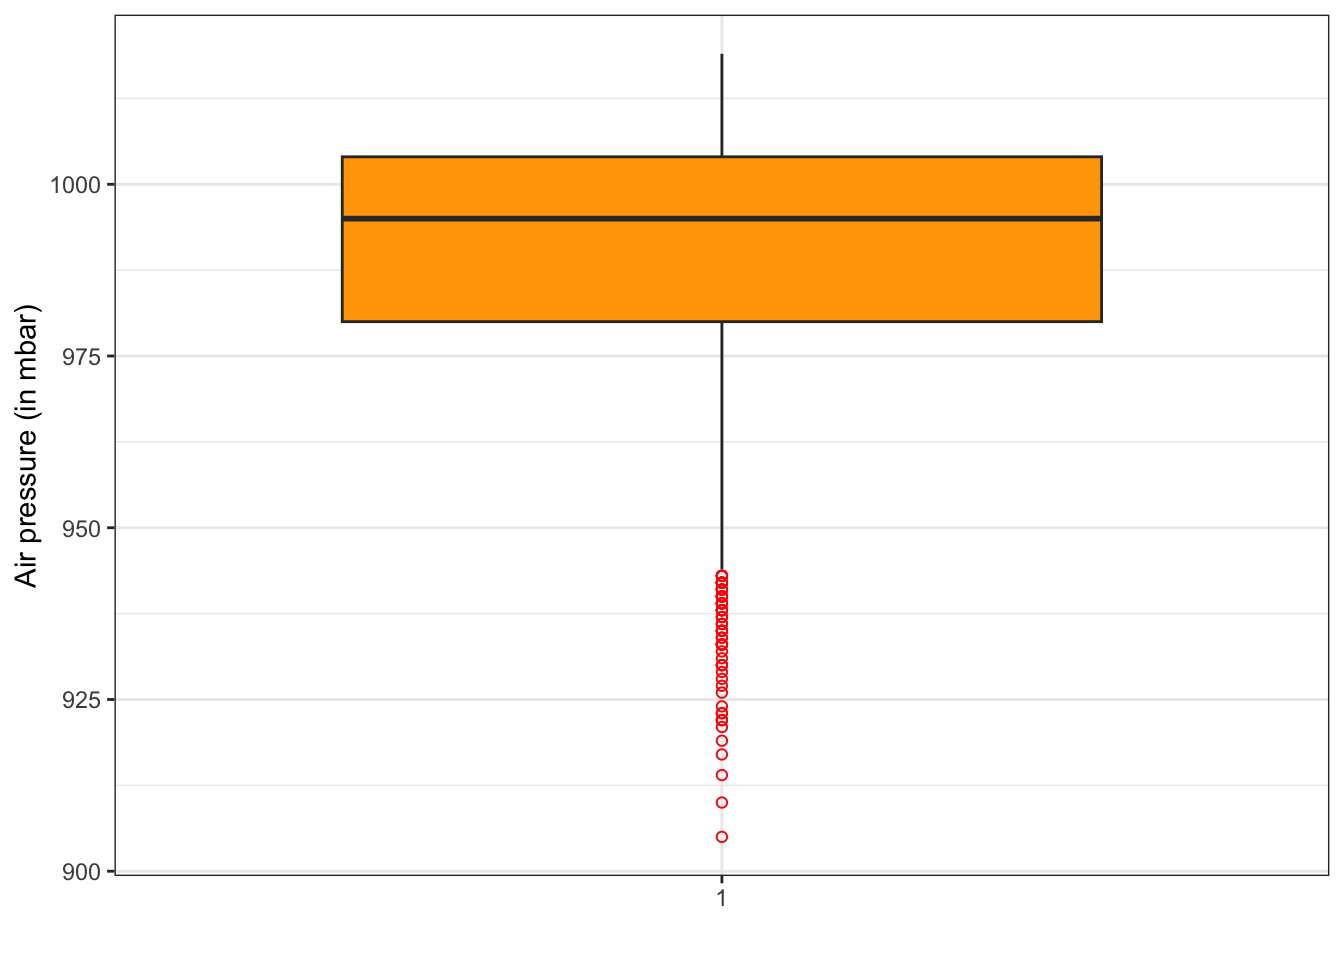
\includegraphics[width=0.95\linewidth]{02-aed_files/figure-latex/aed022-1} 

}

\caption{Gráfico de cajas de la presión atmosférica (versión 2).}\label{fig:aed022}
\end{figure}

Podemos ver que la media se sitúa muy próxima a los 1000 mbar y la gran cantidad de valores extremos en la parte baja de la distribución. Además la caja es muy estrecha indicando la poca variabilidad en los datos, lo que viene corroborado también por la proximidad de los percentiles 25 y 75.

Ahora el gráfico para la variable \texttt{wind}

\begin{Shaded}
\begin{Highlighting}[]
\FunctionTok{ggplot}\NormalTok{(storm, }\FunctionTok{aes}\NormalTok{(}\AttributeTok{x =} \FunctionTok{factor}\NormalTok{(}\DecValTok{1}\NormalTok{),}\AttributeTok{y =}\NormalTok{ wind)) }\SpecialCharTok{+}
   \FunctionTok{geom\_boxplot}\NormalTok{(}\AttributeTok{fill =} \StringTok{"orange"}\NormalTok{,}\AttributeTok{outlier.colour =} \StringTok{"red"}\NormalTok{, }\AttributeTok{outlier.shape =} \DecValTok{1}\NormalTok{) }\SpecialCharTok{+}
   \FunctionTok{scale\_x\_discrete}\NormalTok{(}\AttributeTok{name =} \StringTok{" "}\NormalTok{) }\SpecialCharTok{+} \FunctionTok{scale\_y\_continuous}\NormalTok{(}\AttributeTok{name =} \StringTok{"Wind speed (in knots)"}\NormalTok{) }\SpecialCharTok{+}
   \FunctionTok{theme\_bw}\NormalTok{()}
\end{Highlighting}
\end{Shaded}

\begin{figure}

{\centering 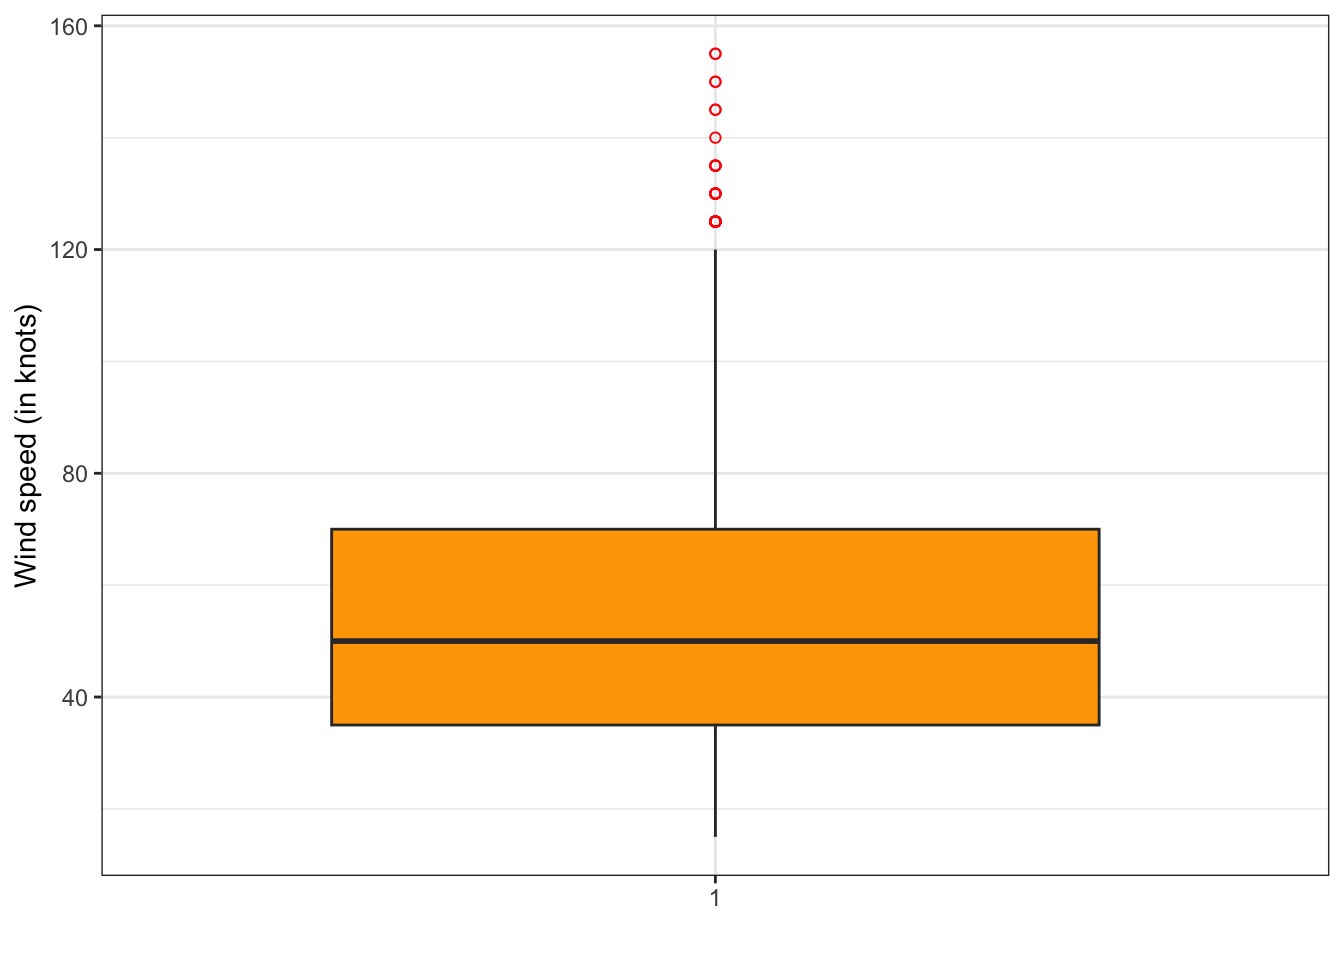
\includegraphics[width=0.95\linewidth]{02-aed_files/figure-latex/aed023-1} 

}

\caption{Gráfico de cajas de la velocidad del viento.}\label{fig:aed023}
\end{figure}

¿Cómo interpretamos este gráfico?

\hypertarget{dos-variables-categuxf3ricas}{%
\subsection{Dos variables categóricas}\label{dos-variables-categuxf3ricas}}

Explorar numéricamente las asociaciones entre pares de variables categóricas no es tan simple como el caso de una variable. La pregunta general que debemos abordar es, ``¿las diferentes combinaciones de categorías parecen estar sub o sobre representadas?''. Necesitamos entender qué combinaciones son comunes y cuáles son raras. Lo más simple que podemos hacer es construir una tabulación cruzada del número de ocurrencias de cada combinación de niveles de ambas variables. La tabla resultante se llama tabla de contingencia.

En cuanto a la representación gráfica la opción más habitual pasa por representar los conteos mediante gráficos de barras que representan de forma conjunta la información de ambas variables.

Para ejemplificar los cálculos y gráficos utilizaremos las variables \texttt{month\_f} (mes como factor) y \texttt{type}. En primer lugar etiquetamos las variables.

\begin{Shaded}
\begin{Highlighting}[]
\CommentTok{\# Etiquetamos las variables}
\NormalTok{storm }\OtherTok{=}\NormalTok{ storm }\SpecialCharTok{\%\textgreater{}\%} 
  \FunctionTok{var\_labels}\NormalTok{(}\AttributeTok{month\_f =} \StringTok{\textquotesingle{}Month\textquotesingle{}}\NormalTok{, }
             \AttributeTok{type =} \StringTok{\textquotesingle{}Storm category\textquotesingle{}}\NormalTok{)}
\end{Highlighting}
\end{Shaded}

\hypertarget{resuxfamenes-numuxe9ricos-2}{%
\subsubsection{Resúmenes numéricos}\label{resuxfamenes-numuxe9ricos-2}}

El resumen numérico habitual para este tipo de situación es la tabla de contigencia (tabla de doble entrada) que nos porporciona los conteos o coincidencias entre los niveles de cada factor. Obtener la tabla completa (frecuencias y porcentajes) puede ser una faena algo pesada utilizando las funciones habituales. En nuestro caso utilizaremos la función \texttt{cross\_tab} de la librería \texttt{pubh}. Dicha función nos porpociona la tbala de doble entrada con los conteos y los porcentajes marginales por columnas. Veamos su uso en el banco de datos.

\begin{Shaded}
\begin{Highlighting}[]
\FunctionTok{table}\NormalTok{(storm}\SpecialCharTok{$}\NormalTok{type, storm}\SpecialCharTok{$}\NormalTok{month\_f)}
\end{Highlighting}
\end{Shaded}

\begin{verbatim}
##                      
##                       June July August September October November December
##   Extratropical         27   38     23       149     129       42        4
##   Hurricane              3   31    300       383     152       25        2
##   Tropical Depression   22   59    150       156      84       42        0
##   Tropical Storm        31  123    247       259     204       61        1
\end{verbatim}

Esta tabla nos permite analizar las concidencias entres los fatores estudiados (conteos), así como la relevancia de cada tipo de tormenta a los largo de los meses estudiados (porcentajes marginales por columnas). Por ejemplo, podemos ver que el perido más activo de huracanes es el comprendido entre los meses de agosto a octubre.

En este caso los porcentajes marginales nos revelan que tipo de tormenta es más habitual dentro de cada mes de los analizados. Por ejemplo, en el mes de agosto el tipo de tormenta más habitual son los huracanes con un 40.1\%, lo que representa casi la mitad de los observado durante ese mes.

\hypertarget{visualizaciuxf3n-gruxe1fica-2}{%
\subsubsection{Visualización gráfica}\label{visualizaciuxf3n-gruxe1fica-2}}

Los gráficos de barras se pueden usar para resumir la relación entre dos variables categóricas. La idea básica es producir una barra separada para cada combinación de categorías en las dos variables. La longitud de estas barras es proporcional a los valores que representan, que son los recuentos brutos o las proporciones en cada combinación de categorías. Esta es la misma información que se muestra en una tabla de contingencia. El uso de ggplot2 para mostrar esta información no es muy diferente de producir un gráfico de barras para resumir una única variable categórica.

Tomamos las variables \texttt{type} y \texttt{year\_f} para mostrar su funcionamiento. Ordenamos la variable \texttt{type} para mostrar los gráficos por orden de importancia de la tormenta. En primer lugar realizamos el gráfico de barras apiladas.

\begin{Shaded}
\begin{Highlighting}[]
\CommentTok{\# Creamos un vector con el orden predefinido}
\NormalTok{ords }\OtherTok{\textless{}{-}} \FunctionTok{c}\NormalTok{(}\StringTok{"Tropical Depression"}\NormalTok{, }\StringTok{"Extratropical"}\NormalTok{, }\StringTok{"Tropical Storm"}\NormalTok{, }\StringTok{"Hurricane"}\NormalTok{)}
\CommentTok{\# Generamos el gráfico indica que el eje x tiene escala dada por el vector ordenado}
\FunctionTok{ggplot}\NormalTok{(storm, }\FunctionTok{aes}\NormalTok{(}\AttributeTok{x =}\NormalTok{ type, }\AttributeTok{fill =}\NormalTok{ year\_f)) }\SpecialCharTok{+} 
  \FunctionTok{geom\_bar}\NormalTok{() }\SpecialCharTok{+} 
  \FunctionTok{scale\_x\_discrete}\NormalTok{(}\AttributeTok{limits =}\NormalTok{ ords) }\SpecialCharTok{+}
  \FunctionTok{xlab}\NormalTok{(}\StringTok{"Storm category"}\NormalTok{) }\SpecialCharTok{+} \FunctionTok{ylab}\NormalTok{(}\StringTok{"Frequancy"}\NormalTok{) }
\end{Highlighting}
\end{Shaded}

\begin{figure}

{\centering 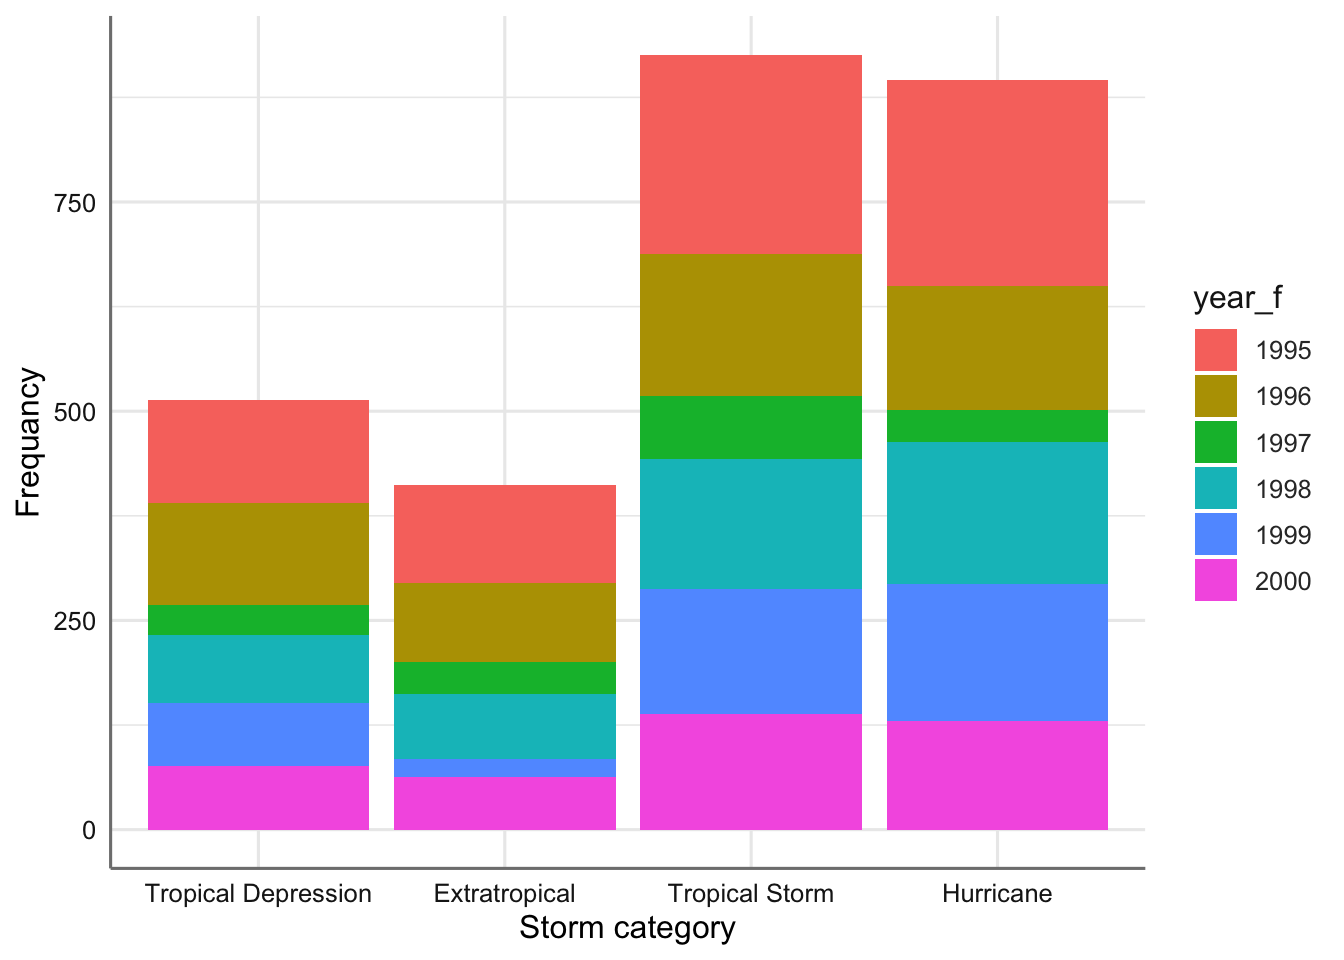
\includegraphics[width=0.95\linewidth]{02-aed_files/figure-latex/aed027-1} 

}

\caption{Gráfico de barras apiladas para tipo de tormenta versus año.}\label{fig:aed027}
\end{figure}

En este caso cada tipo de tormenta tiene su propia barra, y cada barra se ha dividido en diferentes segmentos de colores, cuya longitud está determinada por el número de observaciones asociadas con cada año. Podemos apreciar si para un mismo tipo de tormenta la ocurrencia de un tipo de tormenta es similar o no. Por ejemplo, para los huracanes podemos apreciar que los años 1996, 1998, 1999, y 2000 tienen un número similar de ocurrencias.

Un problema con este tipo de gráfico es que puede ser difícil detectar asociaciones entre las dos variables categóricas. Si queremos saber cómo están asociados, a menudo es mejor trazar los recuentos para cada combinación de categorías una al lado de la otra. Este gráfico se denomina gráfico de barras agrupado. Utilizamos la opción \texttt{dodge} en la función \texttt{geom\_bar} para poder realizar esta versión:

\begin{Shaded}
\begin{Highlighting}[]
\FunctionTok{ggplot}\NormalTok{(storm, }\FunctionTok{aes}\NormalTok{(}\AttributeTok{x =}\NormalTok{ type, }\AttributeTok{fill =}\NormalTok{ year\_f)) }\SpecialCharTok{+} 
  \FunctionTok{geom\_bar}\NormalTok{(}\AttributeTok{position =} \StringTok{"dodge"}\NormalTok{) }\SpecialCharTok{+} 
  \FunctionTok{scale\_x\_discrete}\NormalTok{(}\AttributeTok{limits =}\NormalTok{ ords) }\SpecialCharTok{+}
  \FunctionTok{labs}\NormalTok{(}\AttributeTok{x =} \StringTok{"Storm category"}\NormalTok{, }\AttributeTok{y =} \StringTok{"Frequancy"}\NormalTok{, }\AttributeTok{fill =} \StringTok{"Storm category"}\NormalTok{)}
\end{Highlighting}
\end{Shaded}

\begin{figure}

{\centering 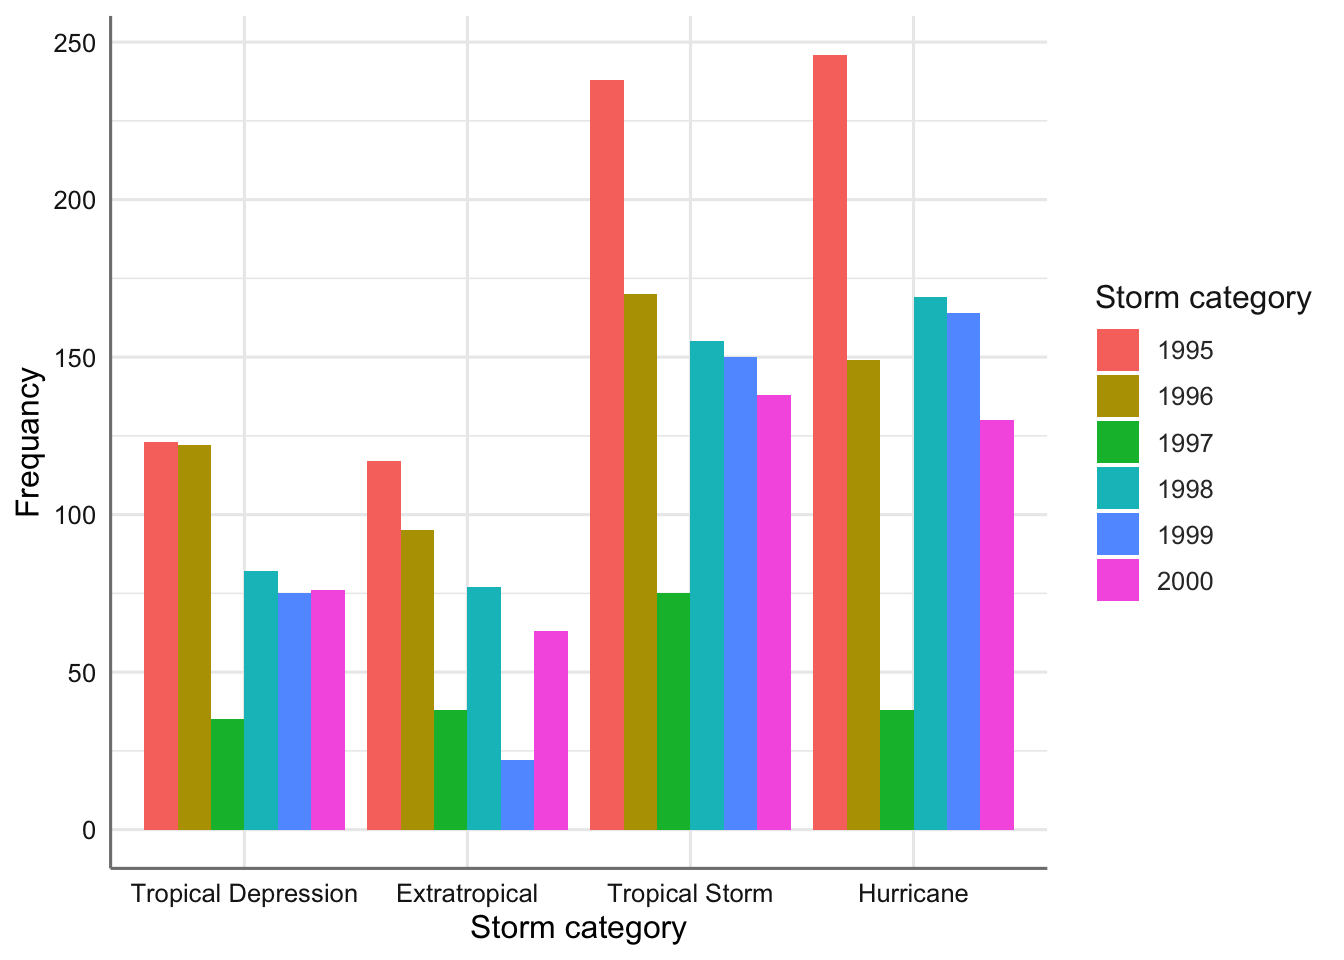
\includegraphics[width=0.95\linewidth]{02-aed_files/figure-latex/aed028-1} 

}

\caption{Gráfico de barras agrupado para el tipo de tormenta versus año.}\label{fig:aed028}
\end{figure}

¿Qué ventajas o desventajas aprecias en este gráfico frente al de barras apiladas?

Alternativamente podríamos realizar el gráfico de porcentahjes en lugar de los conteos. Hacemos uso de la función \texttt{..prop..} e indicamos la agrupación por la variable \texttt{year\_f}:

\begin{Shaded}
\begin{Highlighting}[]
\FunctionTok{ggplot}\NormalTok{(storm, }\FunctionTok{aes}\NormalTok{(}\AttributeTok{x =}\NormalTok{ type, }\AttributeTok{fill =}\NormalTok{ year\_f)) }\SpecialCharTok{+} 
  \FunctionTok{geom\_bar}\NormalTok{(}\FunctionTok{aes}\NormalTok{(}\AttributeTok{y =}\NormalTok{ ..prop.. , }\AttributeTok{group =}\NormalTok{ year\_f),}\AttributeTok{position =} \StringTok{"dodge"}\NormalTok{) }\SpecialCharTok{+} 
  \FunctionTok{scale\_y\_continuous}\NormalTok{(}\AttributeTok{labels =}\NormalTok{ scales}\SpecialCharTok{::}\NormalTok{percent) }\SpecialCharTok{+}
  \FunctionTok{labs}\NormalTok{(}\AttributeTok{x =} \StringTok{"Storm category"}\NormalTok{, }\AttributeTok{y =} \StringTok{"Percent"}\NormalTok{, }\AttributeTok{fill =} \StringTok{"Storm category"}\NormalTok{)}
\end{Highlighting}
\end{Shaded}

\begin{figure}

{\centering 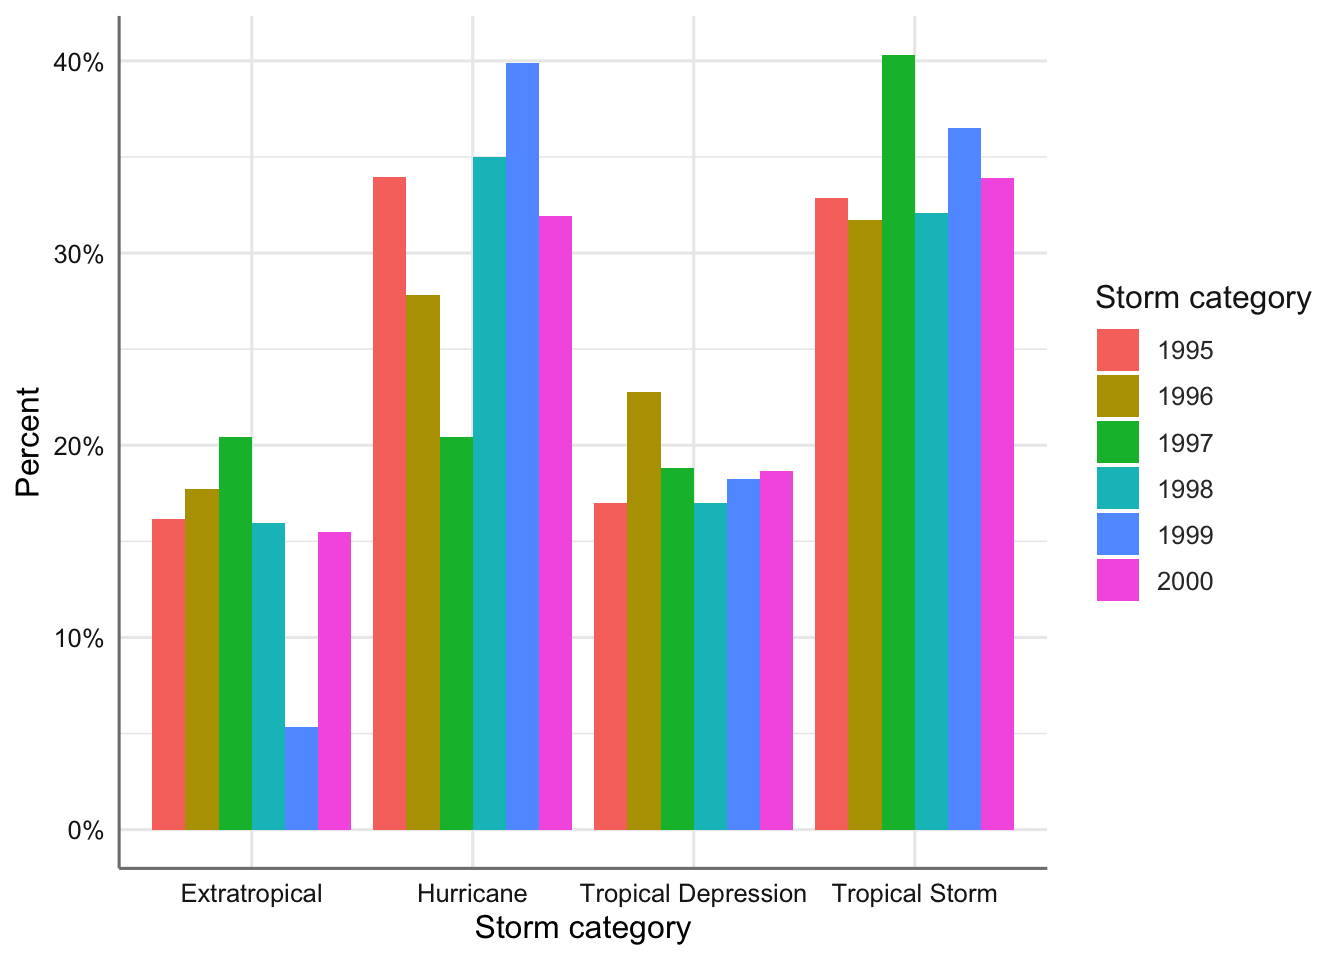
\includegraphics[width=0.95\linewidth]{02-aed_files/figure-latex/aed029-1} 

}

\caption{Gráfico de barras agrupado (porcentjes) para el tipo de tormenta versus año.}\label{fig:aed029}
\end{figure}

Otra opción es realizar un mapa de intensidad de cada una de las combinaciones e ambos factores. Utilizamos la función \texttt{geom\_tile()} a partir los conteos conjuntos para ambas variables con la opción \texttt{count()} que se almacenan en la variable temporal \texttt{n}.

\begin{Shaded}
\begin{Highlighting}[]
\NormalTok{storm }\SpecialCharTok{\%\textgreater{}\%}
    \FunctionTok{count}\NormalTok{(type,year\_f) }\SpecialCharTok{\%\textgreater{}\%}
    \FunctionTok{ggplot}\NormalTok{(}\AttributeTok{mapping =} \FunctionTok{aes}\NormalTok{(}\AttributeTok{x =}\NormalTok{ type, }\AttributeTok{y =}\NormalTok{ year\_f)) }\SpecialCharTok{+} 
        \FunctionTok{geom\_tile}\NormalTok{(}\AttributeTok{mapping =} \FunctionTok{aes}\NormalTok{(}\AttributeTok{fill =}\NormalTok{ n)) }\SpecialCharTok{+} 
        \FunctionTok{scale\_x\_discrete}\NormalTok{(}\AttributeTok{limits =}\NormalTok{ ords) }\SpecialCharTok{+}
        \FunctionTok{labs}\NormalTok{(}\AttributeTok{x =} \StringTok{"Storm type"}\NormalTok{, }\AttributeTok{y =} \StringTok{"Year"}\NormalTok{, }\AttributeTok{fill =} \StringTok{"n"}\NormalTok{)}
\end{Highlighting}
\end{Shaded}

\begin{figure}

{\centering 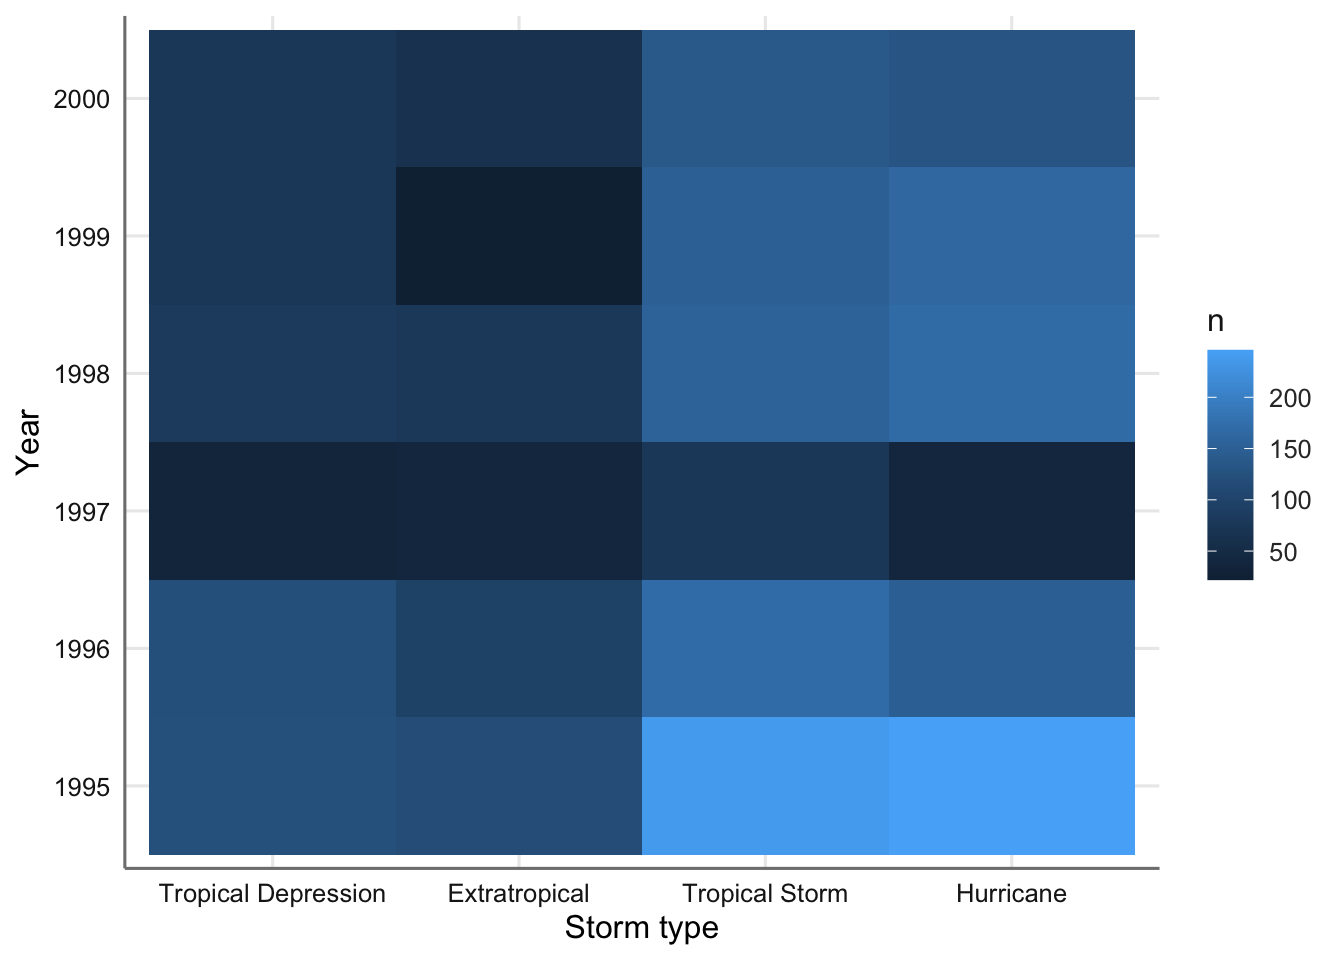
\includegraphics[width=0.95\linewidth]{02-aed_files/figure-latex/aed030-1} 

}

\caption{Mapa de intensidad para el tipo de tormenta versus año.}\label{fig:aed030}
\end{figure}

En este caso las casillas en tonos más claros corresponden con las combinaciones de niveles con una mayor ocurrencia. Las más abundantes se concentran en 1995 y los tipos de tormenta más graves. Por otro lado el año 1997 es el que ha registrado menor número de tormentas.

\hypertarget{categuxf3rica-vs-numuxe9rica}{%
\subsection{Categórica vs Numérica}\label{categuxf3rica-vs-numuxe9rica}}

El objetivo en este tipo de situaciones es comparar cada una de las distribuciones de la variable numérica que surgen al segmentar los valores por cada uno de los niveles de la variable categórica. Tenemos tantas conjuntos de datos como niveles del facgor hemos observado.

\hypertarget{resuxfamenes-numuxe9ricos-3}{%
\subsubsection{Resúmenes numéricos}\label{resuxfamenes-numuxe9ricos-3}}

Los resúmenes numéricos se pueden construir tomando las diversas ideas que hemos explorado para las variables numéricas (medias, medianas, etc.) y aplicándolas a subconjuntos de datos definidos por los valores de la variable categórica. Sin embargo, podemos hacer uso de la función \texttt{estat()} para simplicar este trabajo. para ejemplificar su uso utilizamos la variable \texttt{type} como categórica y las variables \texttt{wind} y \texttt{pressure} como numéricas.

\begin{Shaded}
\begin{Highlighting}[]
\NormalTok{storm}\SpecialCharTok{$}\NormalTok{type }\OtherTok{\textless{}{-}} \FunctionTok{as.factor}\NormalTok{(storm}\SpecialCharTok{$}\NormalTok{type)}
\CommentTok{\# Simplificamos las etiquetas de las variables}
\NormalTok{storm }\OtherTok{=}\NormalTok{ storm }\SpecialCharTok{\%\textgreater{}\%} 
  \FunctionTok{var\_labels}\NormalTok{(}\AttributeTok{wind =} \StringTok{\textquotesingle{}Wind\textquotesingle{}}\NormalTok{, }
             \AttributeTok{pressure =} \StringTok{\textquotesingle{}Air pressure\textquotesingle{}}\NormalTok{)}
\CommentTok{\# Análisis descriptivos}
\FunctionTok{estat}\NormalTok{(}\SpecialCharTok{\textasciitilde{}}\NormalTok{ wind}\SpecialCharTok{|}\NormalTok{type, }\AttributeTok{data =}\NormalTok{ storm)}
\end{Highlighting}
\end{Shaded}

\begin{verbatim}
##                       type   N Min. Max.  Mean Median    SD   CV
## 1 Wind       Extratropical 412   15   80 40.06     40 13.25 0.33
## 2                Hurricane 896   65  155 84.66     80 18.79 0.22
## 3      Tropical Depression 513   20   30 27.36     30  3.52 0.13
## 4           Tropical Storm 926   35  120 47.32     45 11.09 0.23
\end{verbatim}

\begin{Shaded}
\begin{Highlighting}[]
\FunctionTok{estat}\NormalTok{(}\SpecialCharTok{\textasciitilde{}}\NormalTok{ pressure}\SpecialCharTok{|}\NormalTok{type, }\AttributeTok{data =}\NormalTok{ storm)}
\end{Highlighting}
\end{Shaded}

\begin{verbatim}
##                               type   N Min. Max.    Mean Median    SD   CV
## 1 Air pressure       Extratropical 412  950 1019  993.95    996 14.19 0.01
## 2                        Hurricane 896  905 1005  970.44    974 16.95 0.02
## 3              Tropical Depression 513  982 1015 1006.16   1007  3.90 0.00
## 4                   Tropical Storm 926  935 1013  997.70   1000  8.95 0.01
\end{verbatim}

Se puede ver como el tipo Huracanes tiene la media más alta de velocidad del viento y la más baja de presión atmosférica. Además en ambos casos la variabilidad observada es la mayor de todos los tipos de tormenta. La depresión tropical es justo el caso contrario. Evidentemente los datos observados corresponden con la clasificación de tormenta establecida desde el inicio. ¿Qué otras conclusiones podemos obtener? ¿qué tipo de tormenta muestra una mayor variabilidad?

\hypertarget{visualizaciuxf3n-gruxe1fica-3}{%
\subsubsection{Visualización gráfica}\label{visualizaciuxf3n-gruxe1fica-3}}

Para la visualización gráfica de las relaciones entre una variable categórica y una numérica tenemos diferentes opciones: gráfico de densidad, gráfico de cajas, y gráficos comparativos matriciales.

El gráfico de densidad representa la distribución del conjunto de datos muestrales. Con este gráfico se puede apreciar claramente el rango de valores y su concentración (altura de la curva de densidad). Para su obtención utilizamos la opción \texttt{geom\_density()} donde sólo debemos fijar el parámetro de suavizado, \texttt{bw}, que nos indica el grado de información que debemos utilizar para obtener dicha densidad. Valores pequeños dan curvas poco suavizadas y valores grandes dan curva suavizadas. Siempre es necesario un pequeño ajuste para obtener el valor más adecuado. Con este gráfico resulta muy fácil comparar el comportamiento de los diferentes grupos.

Comenzamos con la variable \texttt{wind}:

\begin{Shaded}
\begin{Highlighting}[]
\FunctionTok{ggplot}\NormalTok{(storm, }\FunctionTok{aes}\NormalTok{(}\AttributeTok{x =}\NormalTok{ wind)) }\SpecialCharTok{+} 
  \FunctionTok{geom\_density}\NormalTok{(}\FunctionTok{aes}\NormalTok{(}\AttributeTok{colour =}\NormalTok{ type), }\AttributeTok{bw =} \DecValTok{3}\NormalTok{, }\AttributeTok{na.rm =} \ConstantTok{TRUE}\NormalTok{) }\SpecialCharTok{+} 
  \FunctionTok{labs}\NormalTok{(}\AttributeTok{x =} \StringTok{"Wind speed (in knots)"}\NormalTok{, }\AttributeTok{y =} \StringTok{"Density"}\NormalTok{) }
\end{Highlighting}
\end{Shaded}

\begin{figure}

{\centering 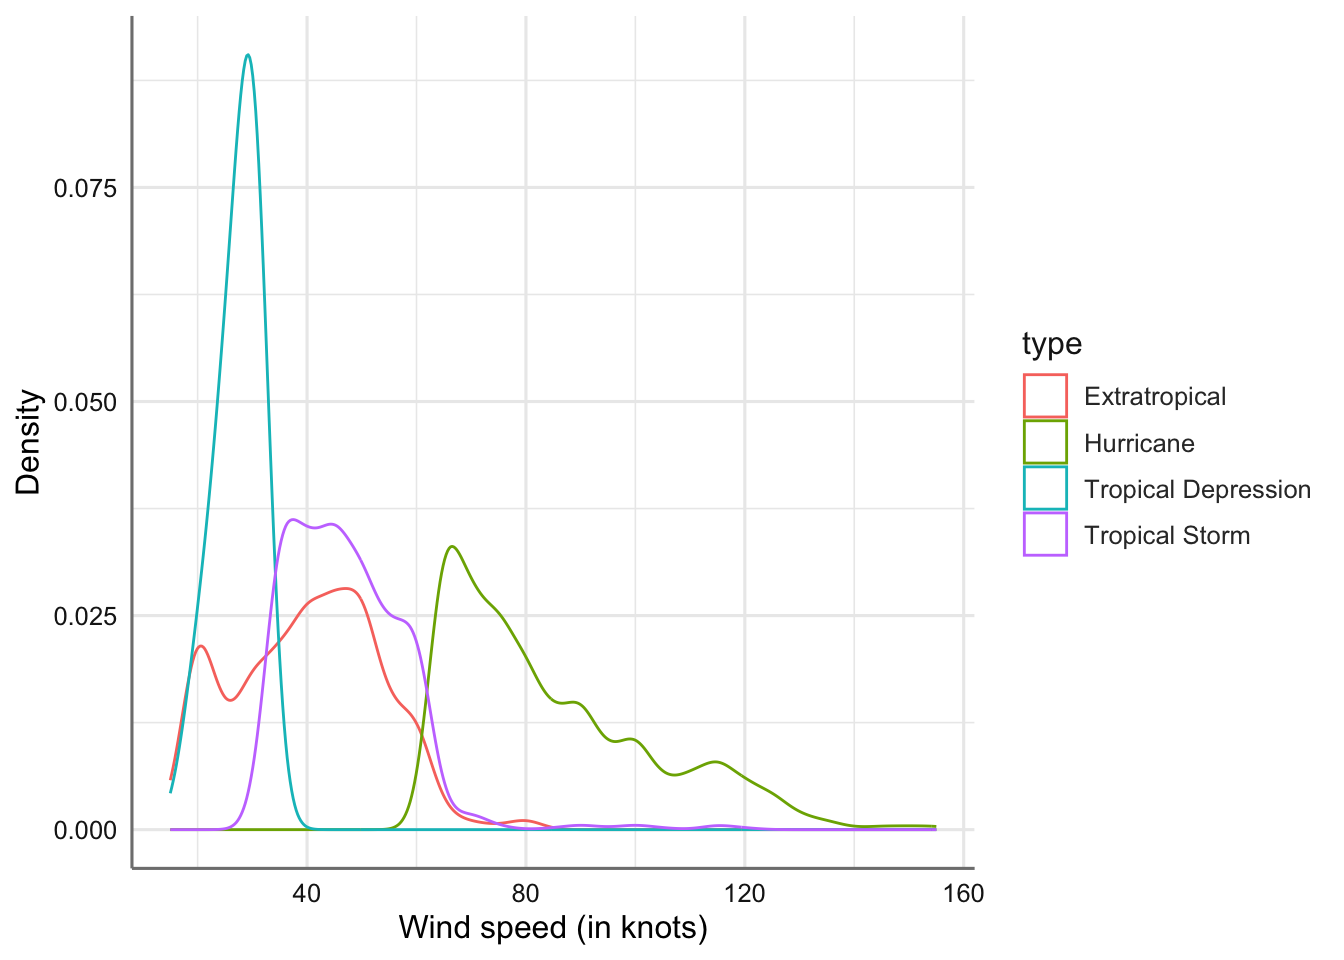
\includegraphics[width=0.95\linewidth]{02-aed_files/figure-latex/aed032-1} 

}

\caption{Gráficos de densidades de la velocidad del viento por tipo de tormenta.}\label{fig:aed032}
\end{figure}

\begin{Shaded}
\begin{Highlighting}[]
\CommentTok{\# la opción na.rm elimina los valores pérdidos.}
\end{Highlighting}
\end{Shaded}

El resultado son cuatro curvas de densidad (una por cada top de tormenta) donde los más destacable es que el rango de valores posibles para la velocidad del viento es sólo diferente para el tipo huracanes, ya que su curva de densidad se encuentra desplazada respecto del resto de densidades. También se puede ver que las depresiones tropicales tienen una menor dispersión (menor rango de valores) los que provoca que su curva sea más puntiaguda. Cuanto mayor sea la dispersión mas amplia sera la densidad obtenida. Si la densidad es simétrica la media se sitúa en el punto medio, mientras que el valor asociado con el punto más alto de la densidad es lo que denominamos moda.

Ahora con la variable presión atmosférica:

\begin{Shaded}
\begin{Highlighting}[]
\FunctionTok{ggplot}\NormalTok{(storm, }\FunctionTok{aes}\NormalTok{(}\AttributeTok{x =}\NormalTok{ pressure)) }\SpecialCharTok{+} 
  \FunctionTok{geom\_density}\NormalTok{(}\FunctionTok{aes}\NormalTok{(}\AttributeTok{colour =}\NormalTok{ type), }\AttributeTok{bw =} \DecValTok{3}\NormalTok{, }\AttributeTok{na.rm =} \ConstantTok{TRUE}\NormalTok{) }\SpecialCharTok{+} 
  \FunctionTok{labs}\NormalTok{(}\AttributeTok{x =} \StringTok{"Air pressure (in knots)"}\NormalTok{, }\AttributeTok{y =} \StringTok{"Density"}\NormalTok{) }
\end{Highlighting}
\end{Shaded}

\begin{figure}

{\centering 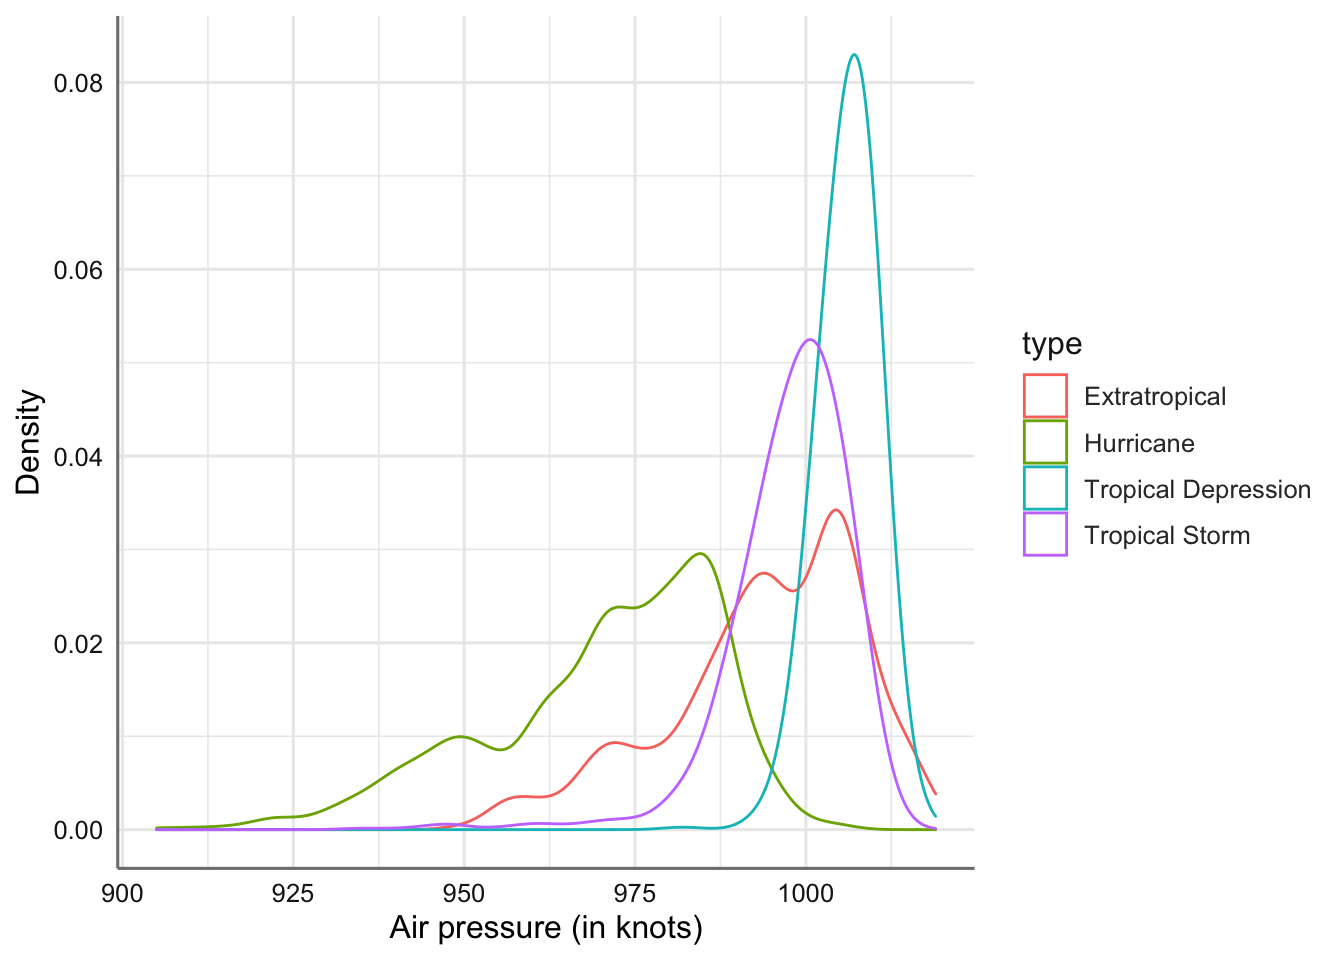
\includegraphics[width=0.95\linewidth]{02-aed_files/figure-latex/aed033-1} 

}

\caption{Gráficos de densidades de la presión atmosférica por tipo de tormenta.}\label{fig:aed033}
\end{figure}

El comportamiento de la variable presión atmosférica es muy similar al de la velocidad del viento pero en la parte izquierda del rango de valores. Los huracanes tienen la menor presión atmosférica y se distinguen del resto de tipos de tormenta. También muestra una mayor variabilidad que el resto de tipos.

La visualización más común para explorar las relaciones entre una variable categórica y otra numérica es el diagrama de cajas. Cada diagrama de caja consiste en:

\begin{itemize}
\tightlist
\item
  Una casilla que se extiende desde el percentil 25 de la distribución hasta el percentil 75, una distancia conocida como rango intercuartílico (IQR). En el medio del recuadro hay una línea que muestra la mediana, es decir, el percentil 50 de la distribución. Estas tres líneas le dan una idea de la extensión de la distribución y si la distribución es simétrica o no respecto a la mediana o sesgada hacia un lado.
\item
  Puntos visuales que muestran observaciones que caen más de 1,5 veces el IQR desde cualquier borde de la caja. Estos puntos remotos son inusuales, por lo que se representan de forma individual.
\item
  Una línea (o bigote) que se extiende desde cada extremo de la caja y va al el punto más lejano no atípico en la distribución.
\end{itemize}

Veamos los ejemplos:

\begin{Shaded}
\begin{Highlighting}[]
\FunctionTok{ggplot}\NormalTok{(storm, }\FunctionTok{aes}\NormalTok{(}\AttributeTok{x =}\NormalTok{ type, }\AttributeTok{y =}\NormalTok{ wind)) }\SpecialCharTok{+} 
  \FunctionTok{geom\_boxplot}\NormalTok{() }\SpecialCharTok{+} 
  \FunctionTok{scale\_x\_discrete}\NormalTok{(}\AttributeTok{limits =}\NormalTok{ ords) }\SpecialCharTok{+}
  \FunctionTok{labs}\NormalTok{(}\AttributeTok{x =} \StringTok{"Storm category"}\NormalTok{, }\AttributeTok{y =} \StringTok{"Wind speed (in knots)"}\NormalTok{) }
\end{Highlighting}
\end{Shaded}

\begin{figure}

{\centering 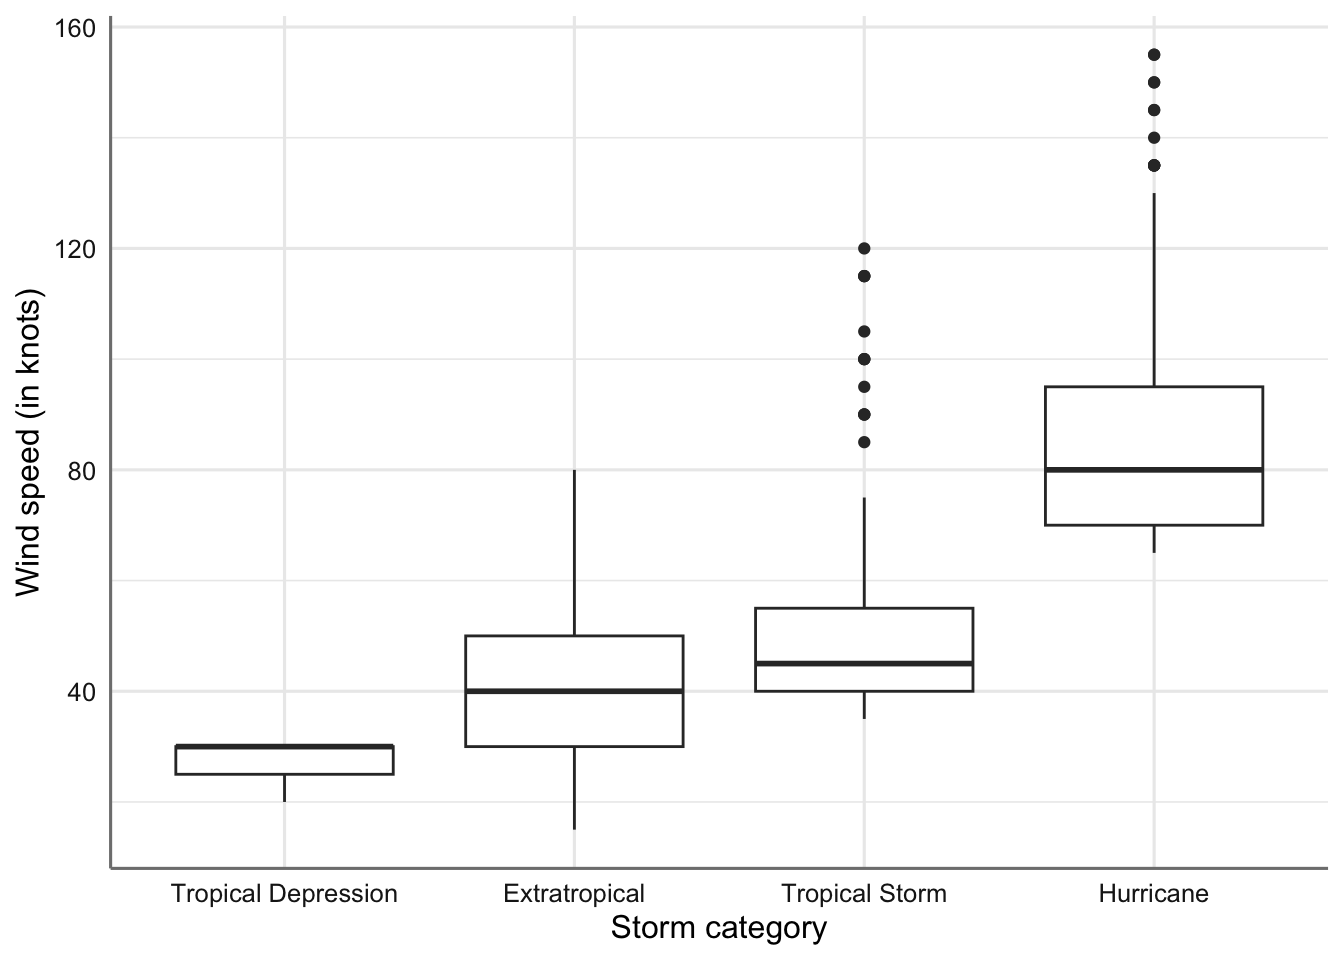
\includegraphics[width=0.95\linewidth]{02-aed_files/figure-latex/aed034-1} 

}

\caption{Gráficos de cajas de la velocidad del viento por tipo de tormenta.}\label{fig:aed034}
\end{figure}

En este tipo de gráficos se esta interesado en dos aspecto fundamentales: * Estudiar la variabilidad dentro de cada grupo viendo la altura de la caja (IQR). * Comparar el comportamiento de cada grupo observando si las cajas quedan a alturas superpuestas.

En este caso podemos ver que la variabilidad más grande se produce en el tipo huracanes y la más pequeña en las depresiones tropicales. Se aprecian diferencias entre las variabilidades de los grupos. Por otro lado, las cajas correspondientes a las tormentas extra tropicales y tormentas tropicales quedan a una misma altura indicando que tienen valores similares para la velocidad del viento. Este gráfico nos da unas primeras indicaciones claras para los procedimientos de comparaciones de medias que estudiaremos más adelante.

\begin{Shaded}
\begin{Highlighting}[]
\FunctionTok{ggplot}\NormalTok{(storm, }\FunctionTok{aes}\NormalTok{(}\AttributeTok{x =}\NormalTok{ type, }\AttributeTok{y =}\NormalTok{ pressure)) }\SpecialCharTok{+} 
  \FunctionTok{geom\_boxplot}\NormalTok{() }\SpecialCharTok{+} 
  \FunctionTok{scale\_x\_discrete}\NormalTok{(}\AttributeTok{limits =}\NormalTok{ ords) }\SpecialCharTok{+}
  \FunctionTok{labs}\NormalTok{(}\AttributeTok{x =} \StringTok{"Storm category"}\NormalTok{, }\AttributeTok{y =} \StringTok{"Air pressure (in mbar)"}\NormalTok{) }
\end{Highlighting}
\end{Shaded}

\begin{figure}

{\centering 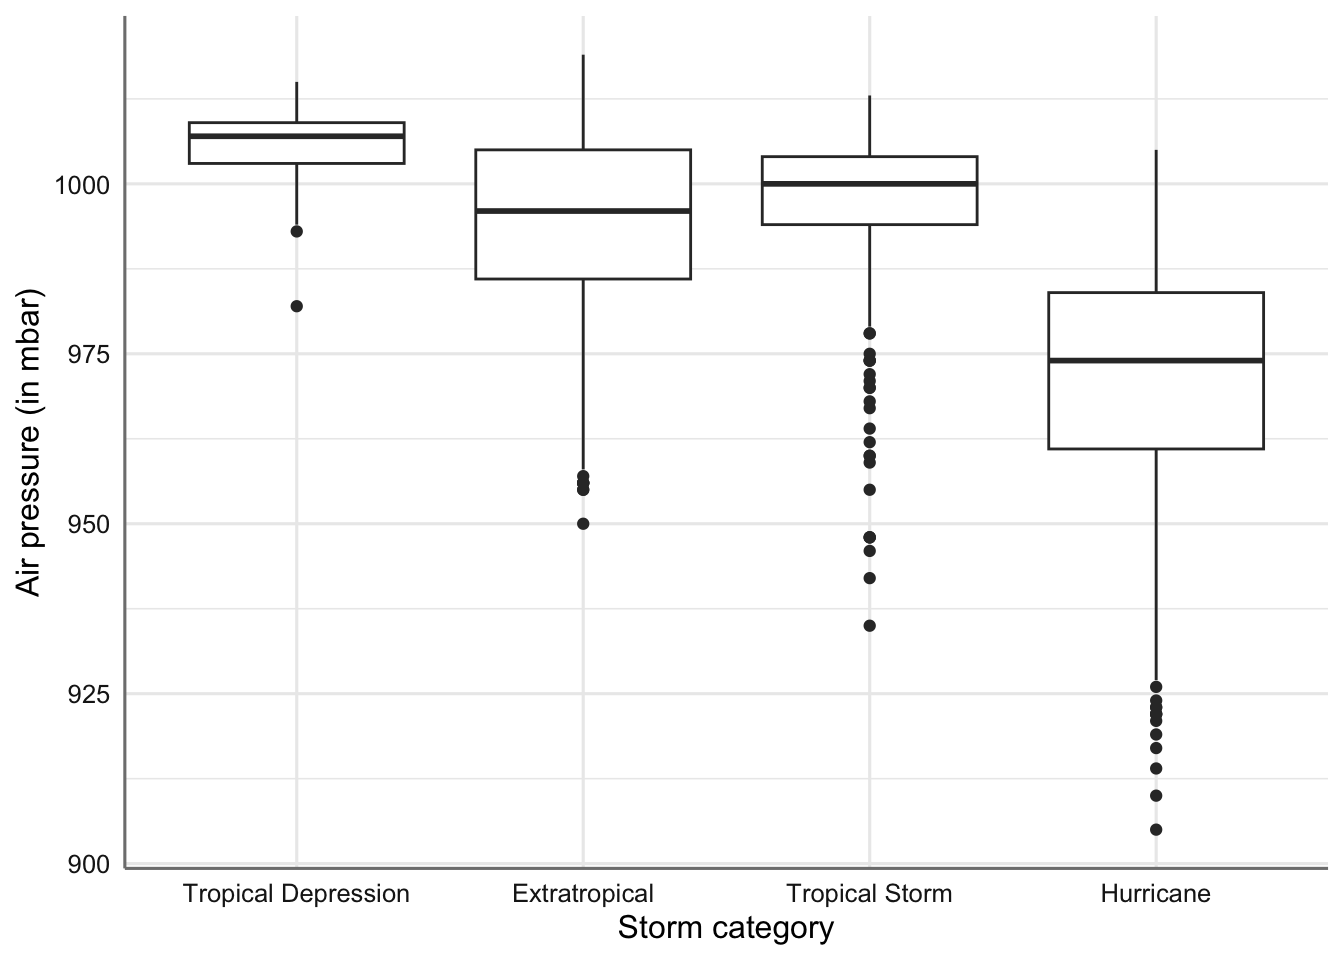
\includegraphics[width=0.95\linewidth]{02-aed_files/figure-latex/aed035-1} 

}

\caption{Gráficos de cajas de la presión atmosférica por tipo de tormenta.}\label{fig:aed035}
\end{figure}

En este caso observamos que los tipos extra tropical y Huracanes muestran variabilidades similares, mientras que los otros dos tipos también muestran variabilidades similares. En cuanto a la comparación de los grupos se observa que el único con un comportamiento diferente son los huracanes. Los otros tres tipos muestran cajas que se podrías solapar mostrando una mayor igualdad en los valores de presión atmosférica.

Los gráficos matriciales o de facetas permiten representar mediante múltiples gráficos la información de una variable numéricas con respecto a los niveles de la variable categórica. Se pretende de esta forma comprobar la forma de la distribución de los datos de forma similar al gráfico de densidad pero realzando un gráfico para cada nivel. Aunque resultan más útiles cuando trabajamos con más de dos variables, se introducen aquí para ir conociendo su funcionamiento en ejemplos sencillos.

Comenzamos realizando un histograma independiente. Para que resulte más fácil visualizar el gráfico introducimos un orden asociado con los valores de la variable numérica, comenzando con el nivel que tiene valores en esa variable más pequeños, y finalizando con la que tiene los valores más grandes.

\begin{Shaded}
\begin{Highlighting}[]
\CommentTok{\# Creamos un nuevo factor ordenado de acuerdo a la variable que estamos midiendo}
\NormalTok{storm}\SpecialCharTok{$}\NormalTok{type2 }\OtherTok{\textless{}{-}} \FunctionTok{reorder}\NormalTok{(storm}\SpecialCharTok{$}\NormalTok{type, storm}\SpecialCharTok{$}\NormalTok{wind)}
\CommentTok{\# Creamos el gráfico}
\FunctionTok{ggplot}\NormalTok{(storm, }\FunctionTok{aes}\NormalTok{(}\AttributeTok{x =}\NormalTok{ wind))  }\SpecialCharTok{+}
  \FunctionTok{geom\_histogram}\NormalTok{(}\AttributeTok{binwidth =} \DecValTok{5}\NormalTok{) }\SpecialCharTok{+} 
  \FunctionTok{xlab}\NormalTok{(}\StringTok{"Wind speed (in knots)"}\NormalTok{) }\SpecialCharTok{+}
  \FunctionTok{ylab}\NormalTok{(}\StringTok{"Frequency"}\NormalTok{) }\SpecialCharTok{+}
  \FunctionTok{facet\_wrap}\NormalTok{(}\SpecialCharTok{\textasciitilde{}}\NormalTok{ type2, }\AttributeTok{ncol =} \DecValTok{1}\NormalTok{)}
\end{Highlighting}
\end{Shaded}

\begin{figure}

{\centering 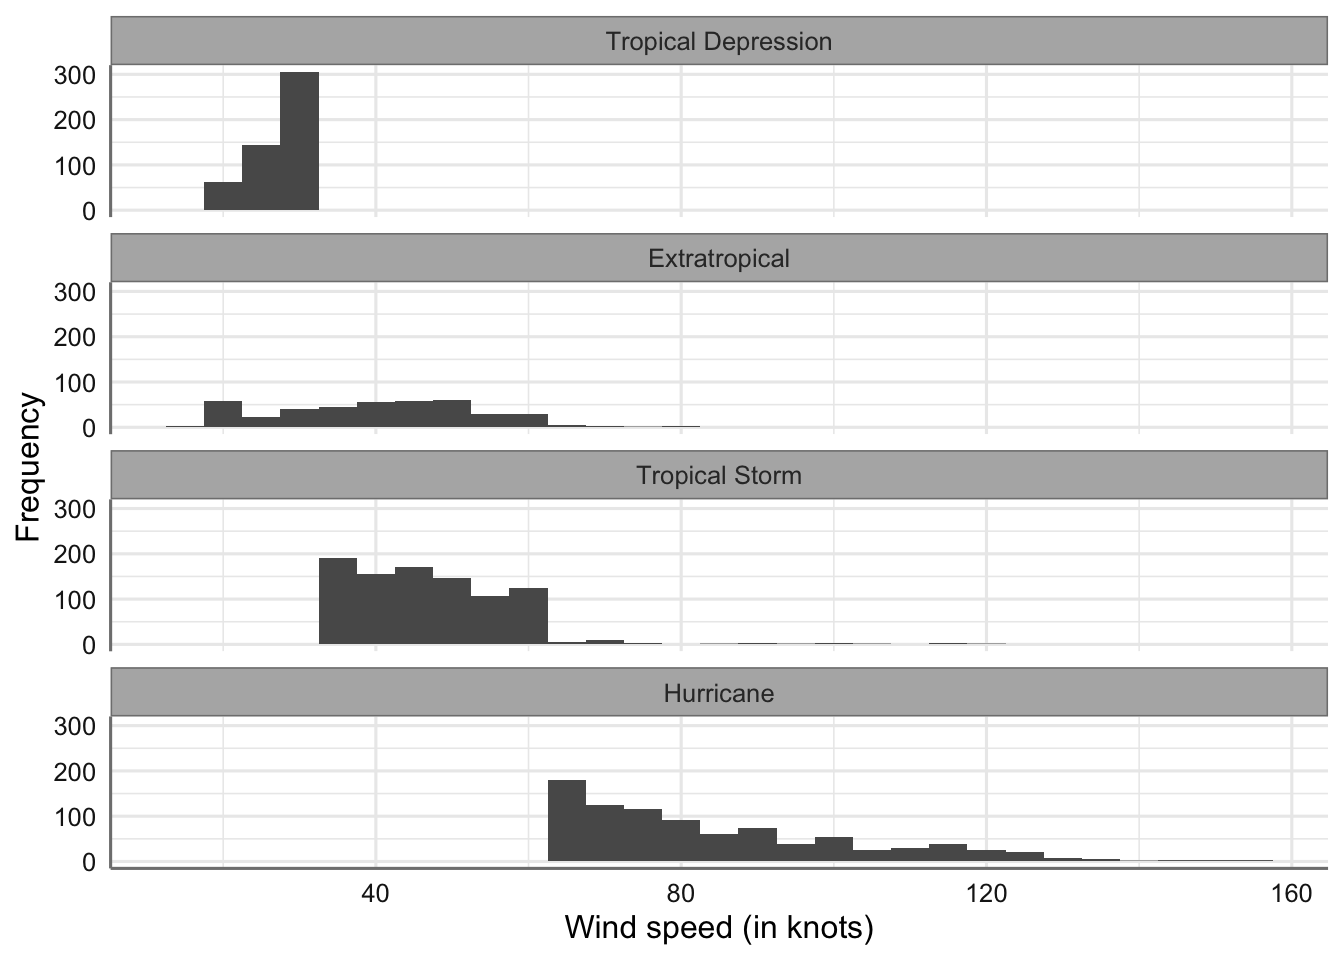
\includegraphics[width=0.95\linewidth]{02-aed_files/figure-latex/aed036-1} 

}

\caption{Gráficos matricial de velocidad del viento por tipo de tormenta}\label{fig:aed036}
\end{figure}

También podríamos realizar el gráfico de densidad

\begin{Shaded}
\begin{Highlighting}[]
\CommentTok{\# Creamos el gráfico}
\FunctionTok{ggplot}\NormalTok{(storm, }\FunctionTok{aes}\NormalTok{(}\AttributeTok{x =}\NormalTok{ wind))  }\SpecialCharTok{+}
  \FunctionTok{geom\_density}\NormalTok{(}\AttributeTok{bw =} \DecValTok{3}\NormalTok{) }\SpecialCharTok{+} 
  \FunctionTok{xlab}\NormalTok{(}\StringTok{"Wind speed (in knots)"}\NormalTok{) }\SpecialCharTok{+}
  \FunctionTok{ylab}\NormalTok{(}\StringTok{"Density"}\NormalTok{) }\SpecialCharTok{+}
  \FunctionTok{facet\_wrap}\NormalTok{(}\SpecialCharTok{\textasciitilde{}}\NormalTok{ type2, }\AttributeTok{ncol =} \DecValTok{1}\NormalTok{)}
\end{Highlighting}
\end{Shaded}

\begin{figure}

{\centering 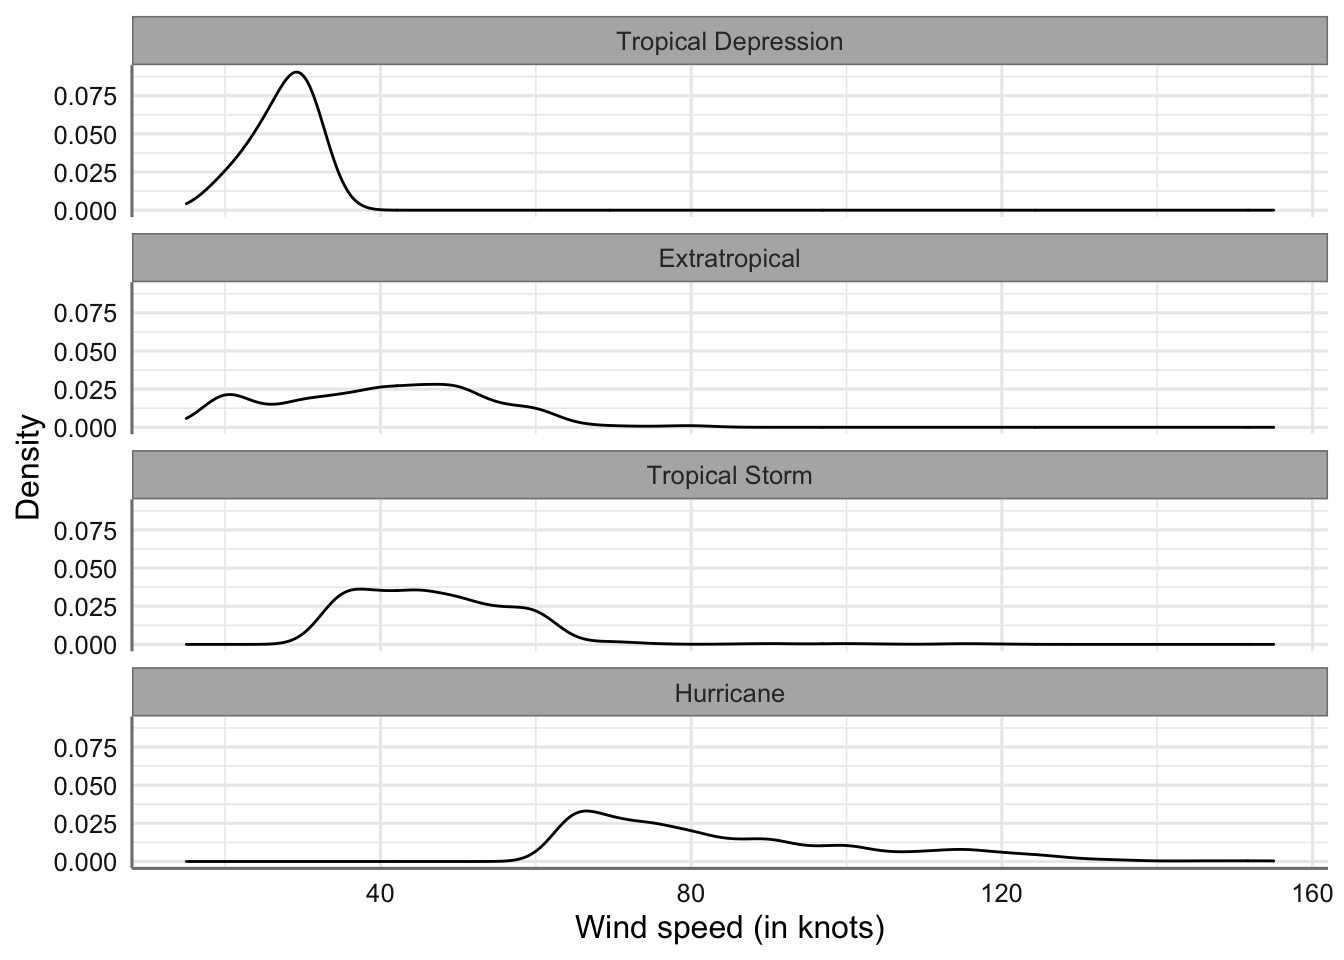
\includegraphics[width=0.95\linewidth]{02-aed_files/figure-latex/aed037-1} 

}

\caption{Gráficos matricial de velocidad del viento por tipo de tormenta}\label{fig:aed037}
\end{figure}

En ambos casos las interpretaciones son similares a las que se hicieron con el gráfico conjunto de densidad.

Podemos cambiar la configuración cambiando el número de columnas:

\begin{Shaded}
\begin{Highlighting}[]
\CommentTok{\# Creamos el gráfico}
\FunctionTok{ggplot}\NormalTok{(storm, }\FunctionTok{aes}\NormalTok{(}\AttributeTok{x =}\NormalTok{ wind))  }\SpecialCharTok{+}
  \FunctionTok{geom\_density}\NormalTok{(}\AttributeTok{bw =} \DecValTok{3}\NormalTok{) }\SpecialCharTok{+} 
  \FunctionTok{xlab}\NormalTok{(}\StringTok{"Wind speed (in knots)"}\NormalTok{) }\SpecialCharTok{+}
  \FunctionTok{ylab}\NormalTok{(}\StringTok{"Density"}\NormalTok{) }\SpecialCharTok{+}
  \FunctionTok{facet\_wrap}\NormalTok{(}\SpecialCharTok{\textasciitilde{}}\NormalTok{ type2, }\AttributeTok{ncol =} \DecValTok{2}\NormalTok{)}
\end{Highlighting}
\end{Shaded}

\begin{figure}

{\centering 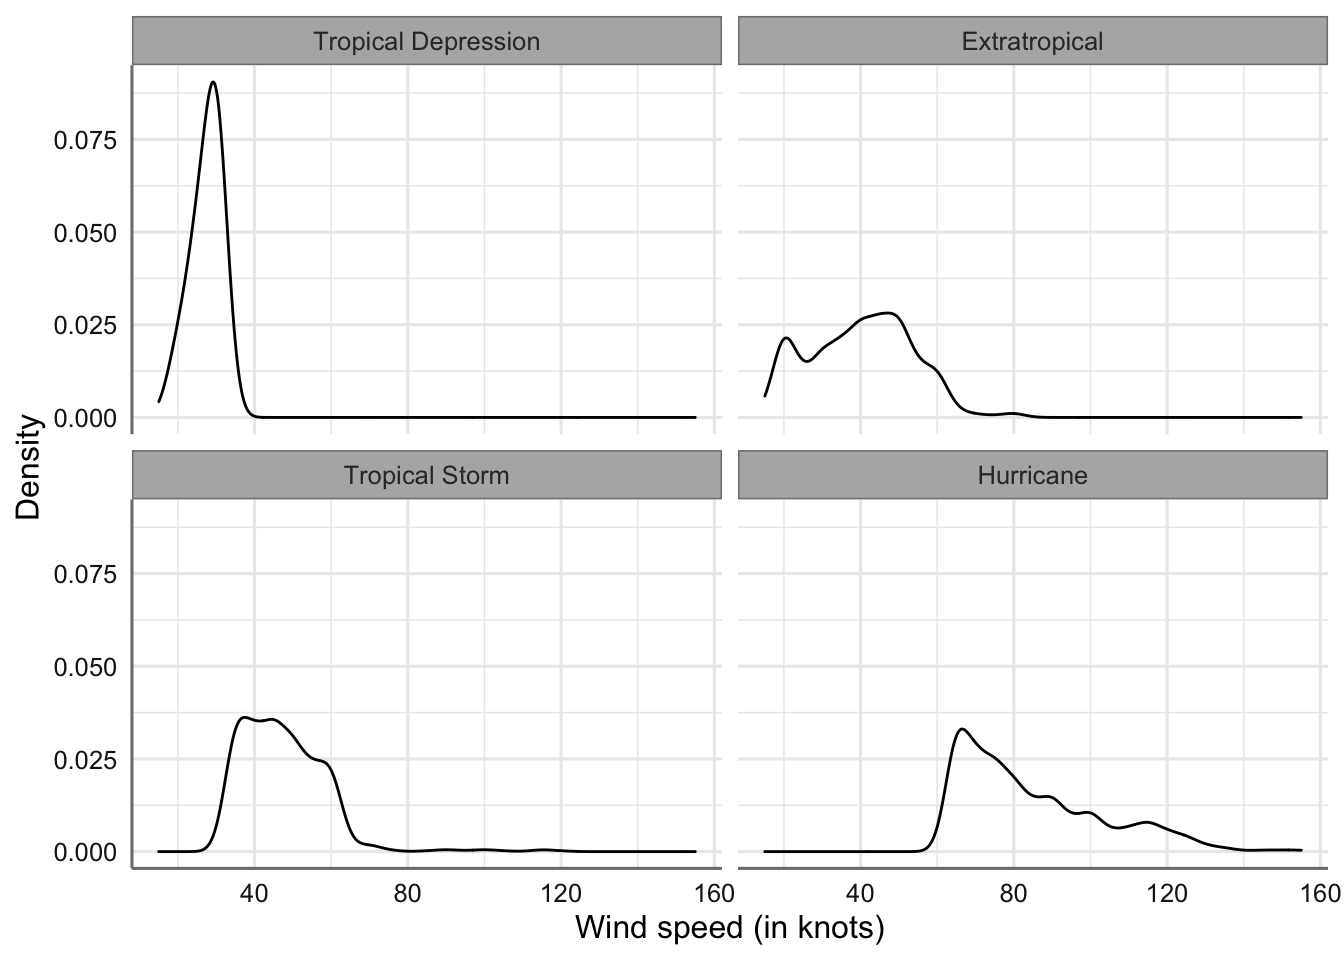
\includegraphics[width=0.95\linewidth]{02-aed_files/figure-latex/aed038-1} 

}

\caption{Gráficos matricial de velocidad del viento por tipo de tormenta}\label{fig:aed038}
\end{figure}

Aunque el gráfico se visualiza mejor también resulta más difícil la comparación entre todos los niveles.

Si deseamos cambiar la situación de las etiquetas del factor podemos utilizar la opción \texttt{facet\_grid}.

\begin{Shaded}
\begin{Highlighting}[]
\CommentTok{\# Creamos el gráfico}
\FunctionTok{ggplot}\NormalTok{(storm, }\FunctionTok{aes}\NormalTok{(}\AttributeTok{x =}\NormalTok{ wind))  }\SpecialCharTok{+}
  \FunctionTok{geom\_density}\NormalTok{(}\AttributeTok{bw =} \DecValTok{3}\NormalTok{) }\SpecialCharTok{+} 
  \FunctionTok{xlab}\NormalTok{(}\StringTok{"Wind speed (in knots)"}\NormalTok{) }\SpecialCharTok{+}
  \FunctionTok{ylab}\NormalTok{(}\StringTok{"Density"}\NormalTok{) }\SpecialCharTok{+}
  \FunctionTok{facet\_grid}\NormalTok{(type2 }\SpecialCharTok{\textasciitilde{}}\NormalTok{ .)}
\end{Highlighting}
\end{Shaded}

\begin{figure}

{\centering 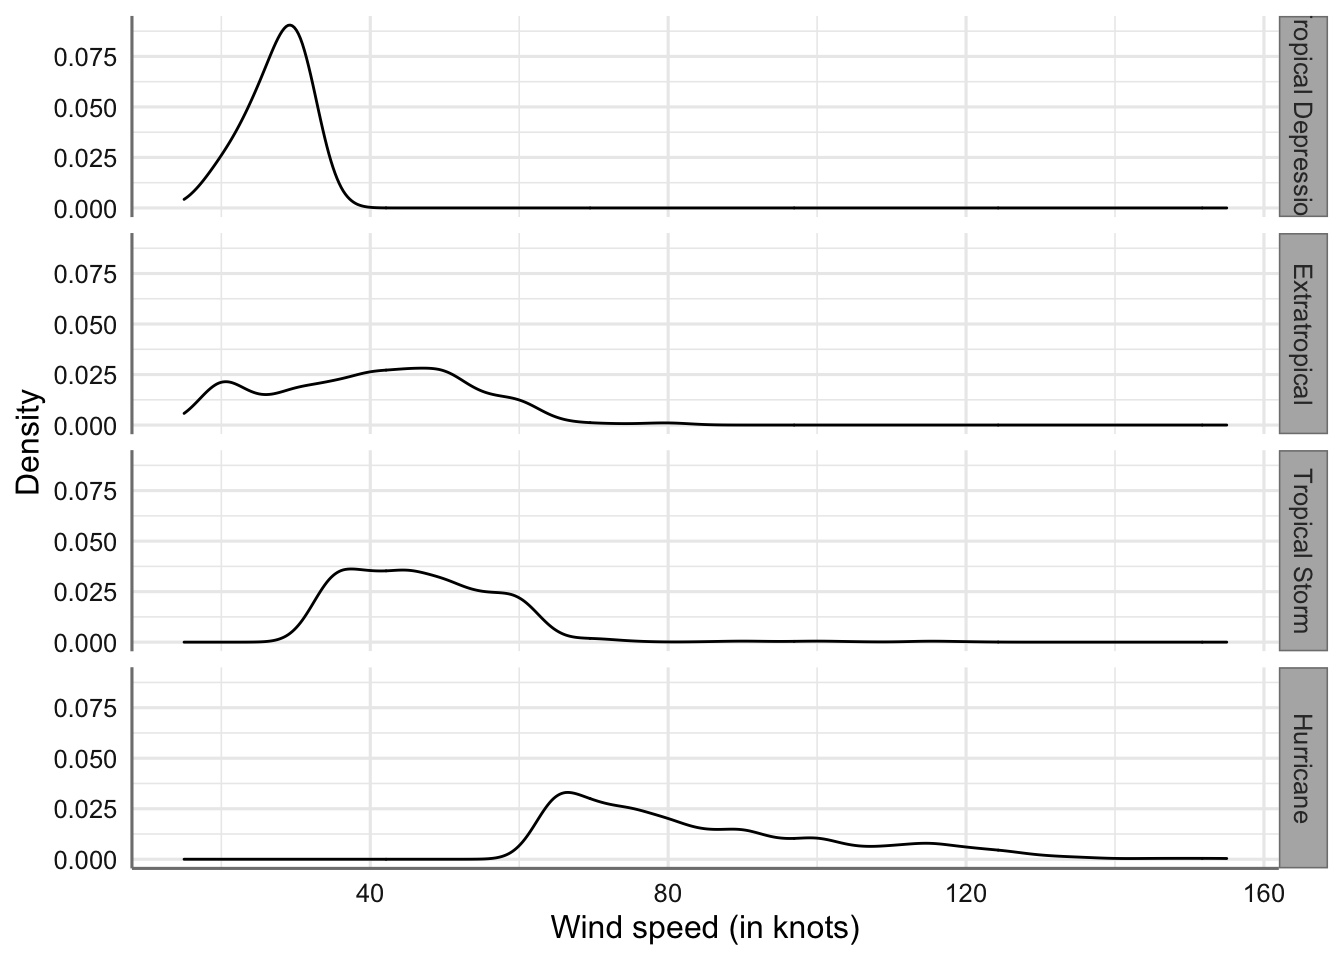
\includegraphics[width=0.95\linewidth]{02-aed_files/figure-latex/aed039-1} 

}

\caption{Gráficos matricial (grid) de velocidad del viento por tipo de tormenta}\label{fig:aed039}
\end{figure}

Esta opción nos resultará de mayor utilidad cuando tengamos que representar dos factores ya que se podrá situar en la filas uno de los factores y el otro en las columnas con la opción \texttt{facet\_grid(factor1\ \textasciitilde{}\ factor2)}.

\hypertarget{dos-variables-numuxe9ricas}{%
\subsection{Dos variables numéricas}\label{dos-variables-numuxe9ricas}}

Los estadísticos han ideado varias formas diferentes de cuantificar la asociación entre dos variables numéricas en un banco de datos. Las medidas más comunes medidas buscan calcular algún tipo de coeficiente de asociación Los términos ``asociación'' y ``correlación'' están estrechamente relacionados; tanto que a menudo se usan indistintamente. La más habitual es la correlación lineal que cuantifica el grado de asociación lineal entre dos variables de tipo numérico. Para ejemplificar nuestros cálculos y gráficos utilizaremos las variables \texttt{wind} y \texttt{preassure}.

\hypertarget{resuxfamenes-numuxe9ricos-4}{%
\subsubsection{Resúmenes numéricos}\label{resuxfamenes-numuxe9ricos-4}}

La medida de correlación más utilizada es el coeficiente de correlación lineal de Pearson. El coeficiente de correlación de Pearson cuantifica el grado de asociación entre las variables en la escala -1 a 1, donde -1 indica una relación inversa (cuando una variable crece la otra decrece) y 1 indica una relación directa (cuando una crece la otra también lo hace. Valores próximo a cero indican que no hay asociación lineal entre las variables analizadas. Este coeficiente es la base para plantear lo que denominaremos más adelante los modelos de regresión lineal simple.

La definición formal del coeficiente de correlación de Pearson (\(\rho\)) viene dada por: \begin{equation} 
  \rho = \frac{1}{n-1}\sum_{i=1}^n \frac{(x_i - \bar{x})(y_i - \bar{y})}{s_x s_y}
  \label{eq:coefcorrel}
\end{equation}

donde \(x_i\), \(y_i\) son las observaciones de la variable \(x\) e \(y\) respectivamente, \(\bar{x}\), \(\bar{y}\) son las medias muestrales de cada variable, y \(s_x\), \(s_y\) son las desviaciones típica de cada variable. El coeficiente trata de valorar la ``covaraición'' entre ambas variables, es decir, como afectan los cambios de valores en una variable en los valores de la otra, teniendo en cuenta la propia variabilidad de cada una de ellas.

Para obtener el coeficiente de correlación utilizamos la función \texttt{cor()}.

\begin{Shaded}
\begin{Highlighting}[]
\FunctionTok{cor}\NormalTok{(storm}\SpecialCharTok{$}\NormalTok{wind,storm}\SpecialCharTok{$}\NormalTok{pressure)}
\end{Highlighting}
\end{Shaded}

\begin{verbatim}
## [1] -0.9254911
\end{verbatim}

El coeficiente de correlación resulta negativo, lo que indica que la velocidad del viento tiende a disminuir al aumentar la presión. Al estar próximo a -1 se puede intuir que dicha asociación es muy fuerte. Sin embargo, el coeficiente de correlación de Pearson debe interpretarse con cuidado debido a que está diseñado para medir una relación de tipo lineal, lo que implica que dicho coeficiente será engañoso cuando esta relación sea curva, o incluso peor, en forma de joroba.

¿Qué deberíamos hacer si pensamos que la relación entre dos variables no es lineal? No deberíamos usar el coeficiente de correlación de Pearson para medir la asociación en este caso. En cambio, podemos calcular lo que denominamos correlación de rango. La idea es muy simple. En lugar de trabajar con los valores reales de cada variable, los ``clasificamos'', es decir, ordenamos cada variable de menor a mayor y asignamos las etiquetas ``primero'', ``segundo'', ``tercero'', etc. a diferentes observaciones. Las medidas de correlación de rangos se basan en una comparación de los rangos resultantes. Los dos más populares son Spearman's y Kendall's. Ambos coeficientes se comportan de una manera muy similar al coeficiente de correlación de Pearson. Toman un valor de 0 si los rangos no están correlacionados, y un valor de +1 o -1 si están perfectamente relacionados.

Podemos calcular ambos coeficientes de correlación de rangos en R usando nuevamente la función cor. Esta vez necesitamos establecer el argumento del método en el valor apropiado: \texttt{method\ =\ "kendall"} o \texttt{method\ =\ "spearman"}.

\begin{Shaded}
\begin{Highlighting}[]
\FunctionTok{cor}\NormalTok{(storm}\SpecialCharTok{$}\NormalTok{wind,storm}\SpecialCharTok{$}\NormalTok{pressure,}\AttributeTok{method =} \StringTok{"kendall"}\NormalTok{)}
\end{Highlighting}
\end{Shaded}

\begin{verbatim}
## [1] -0.7627645
\end{verbatim}

\begin{Shaded}
\begin{Highlighting}[]
\FunctionTok{cor}\NormalTok{(storm}\SpecialCharTok{$}\NormalTok{wind,storm}\SpecialCharTok{$}\NormalTok{pressure,}\AttributeTok{method =} \StringTok{"spearman"}\NormalTok{)}
\end{Highlighting}
\end{Shaded}

\begin{verbatim}
## [1] -0.9025831
\end{verbatim}

Los resultados obtenidos son compatibles con el del coeficiente de Pearson.

\hypertarget{visualizaciuxf3n-gruxe1fica-4}{%
\subsubsection{Visualización gráfica}\label{visualizaciuxf3n-gruxe1fica-4}}

Los coeficientes de correlación nos dan una forma simple de resumir las asociaciones entre variables numéricas. Sin embargo, son limitados, porque un solo número nunca puede resumir todos los aspectos de la relación entre dos variables. Es por eso que siempre visualizamos la relación entre dos variables. El gráfico estándar para mostrar asociaciones entre variables numéricas es un diagrama de dispersión, usando ejes horizontales y verticales para trazar dos variables como una serie de puntos. Para realizar este gráfico usamos la opción \texttt{geom\_point()}

\begin{Shaded}
\begin{Highlighting}[]
\FunctionTok{ggplot}\NormalTok{(storm, }\FunctionTok{aes}\NormalTok{(}\AttributeTok{x =}\NormalTok{ wind, }\AttributeTok{y =}\NormalTok{ pressure)) }\SpecialCharTok{+} 
  \FunctionTok{geom\_point}\NormalTok{() }\SpecialCharTok{+} 
  \FunctionTok{labs}\NormalTok{(}\AttributeTok{x =} \StringTok{"Wind speed (in knots)"}\NormalTok{, }\AttributeTok{y =} \StringTok{"Air pressure (in mbar)"}\NormalTok{)}
\end{Highlighting}
\end{Shaded}

\begin{figure}

{\centering 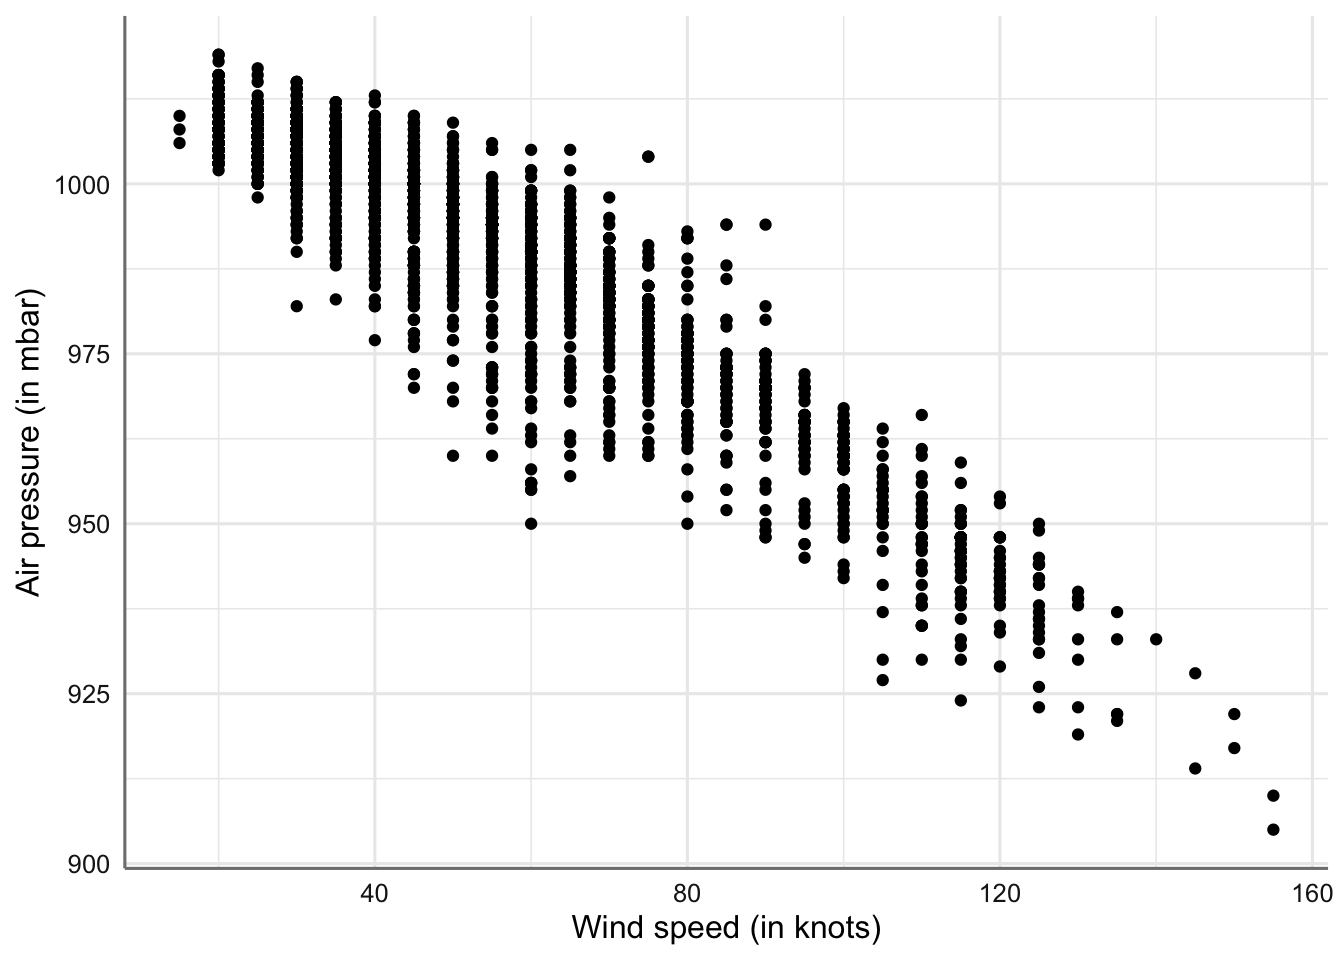
\includegraphics[width=0.95\linewidth]{02-aed_files/figure-latex/aed042-1} 

}

\caption{Gráfico de dispersión de velocidad del viento vs presión atmosférica}\label{fig:aed042}
\end{figure}

En el gráfico se puede apreciar la relación de tipo lineal en orden o pendiente decreciente (cuando aumenta el viento disminuye la presión).

El problema de este gráfico es que no podemos apreciar todos los puntos, ya que si tenemos dos observaciones con los mismo valores en ambas variables, estos quedarían superpuestos. Para solucionar esta deficiencia podemos optar por otra versión del gráfico de dispersión que nos permita contabilizar el número de repeticiones cuando estas existan. Este gráfico se obtiene con la opción \texttt{geom\_hex()}. Para poder realizarlo es necesario instalar la librería \texttt{hexbin}:

\begin{Shaded}
\begin{Highlighting}[]
\FunctionTok{ggplot}\NormalTok{(storm, }\FunctionTok{aes}\NormalTok{(}\AttributeTok{x =}\NormalTok{ wind, }\AttributeTok{y =}\NormalTok{ pressure)) }\SpecialCharTok{+} 
  \FunctionTok{geom\_hex}\NormalTok{(}\AttributeTok{bins =} \DecValTok{25}\NormalTok{) }\SpecialCharTok{+} 
        \FunctionTok{labs}\NormalTok{(}\AttributeTok{x =} \StringTok{"Wind speed (in knots)"}\NormalTok{, }\AttributeTok{y =} \StringTok{"Air pressure (in mbar)"}\NormalTok{, }\AttributeTok{fill =} \StringTok{"n"}\NormalTok{)}
\end{Highlighting}
\end{Shaded}

\begin{figure}

{\centering 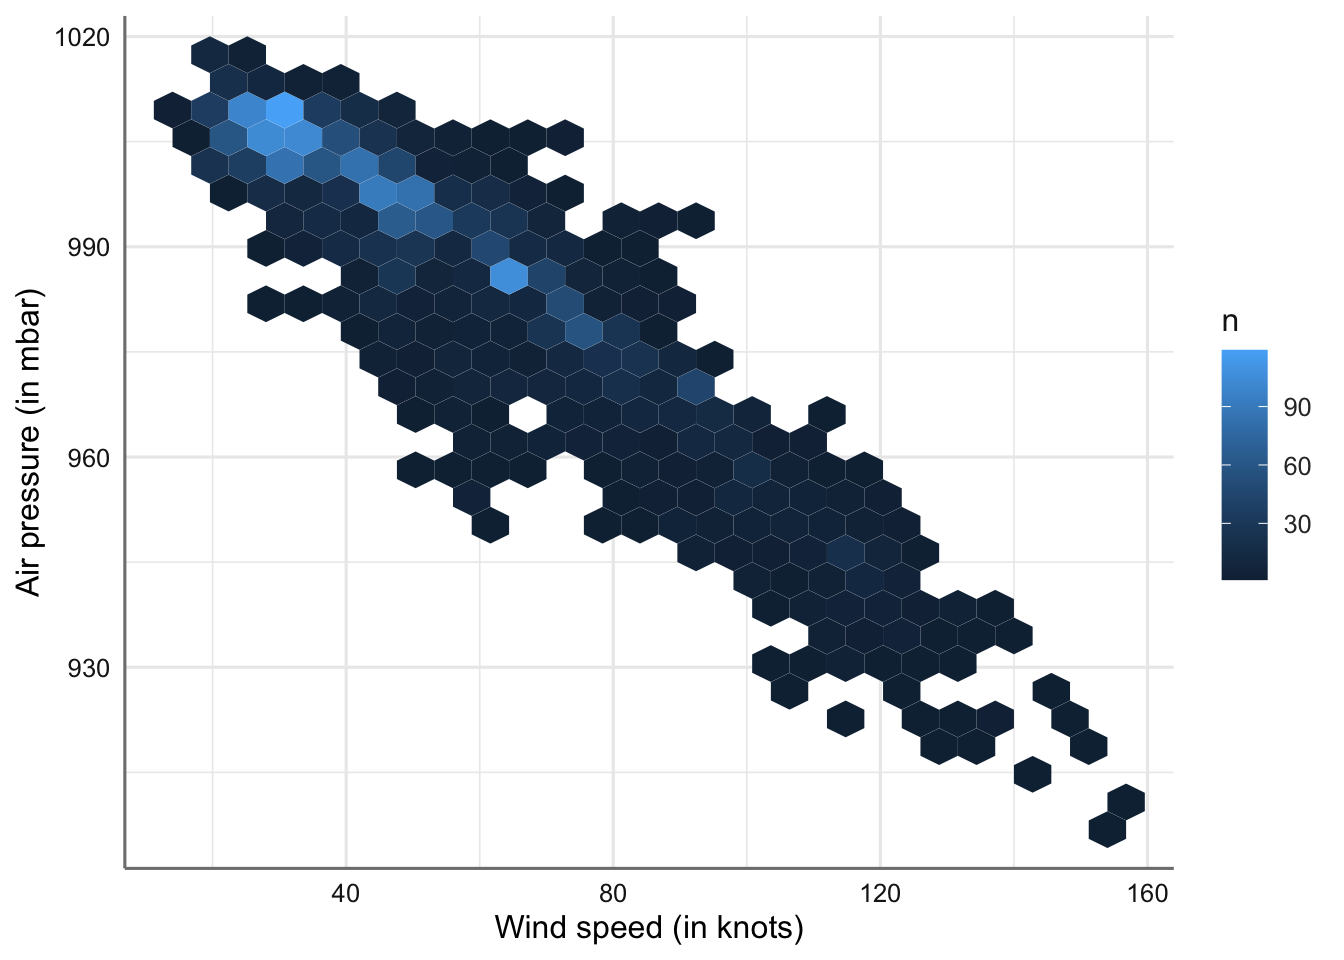
\includegraphics[width=0.95\linewidth]{02-aed_files/figure-latex/aed043-1} 

}

\caption{Gráfico de dispersión de velocidad del viento vs presión atmosférica (versión dos).}\label{fig:aed043}
\end{figure}

El parámetro \texttt{bins} segmenta el rango de cada variable en intervalos disjuntos. Lo que se representa es una gráfico de dispersión por intervalos, de forma que cada casilla representa todos los valores que quedan dentro del intervalo conjunto que obtenemos con ambas variables. Se observa que la tendencia se mantiene pero resulta posible ver que valores muestran una mayor o menor ocurrencia. La combinación de valores bajos de viento (\textless{} 40 mph) con altos de presión (\textgreater{} 990 mb) son los que más aparecen en el banco de datos.

Otra opción es agrupar una variable continua para que actúe como una variable categórica. Luego se puede usar un gráfico combinado de cajas para representar ambas variables Veamos un ejemplo:

\begin{Shaded}
\begin{Highlighting}[]
\FunctionTok{ggplot}\NormalTok{(}\AttributeTok{data =}\NormalTok{ storm, }\FunctionTok{aes}\NormalTok{(}\AttributeTok{x =}\NormalTok{ wind, }\AttributeTok{y =}\NormalTok{ pressure)) }\SpecialCharTok{+} 
  \FunctionTok{geom\_boxplot}\NormalTok{(}\AttributeTok{mapping =} \FunctionTok{aes}\NormalTok{(}\AttributeTok{group =} \FunctionTok{cut\_width}\NormalTok{(wind, }\DecValTok{10}\NormalTok{))) }\SpecialCharTok{+} 
        \FunctionTok{labs}\NormalTok{(}\AttributeTok{x =} \StringTok{"Wind speed (in knots)"}\NormalTok{, }\AttributeTok{y =} \StringTok{"Air pressure (in mbar)"}\NormalTok{, }\AttributeTok{fill =} \StringTok{"n"}\NormalTok{)}
\end{Highlighting}
\end{Shaded}

\begin{figure}

{\centering 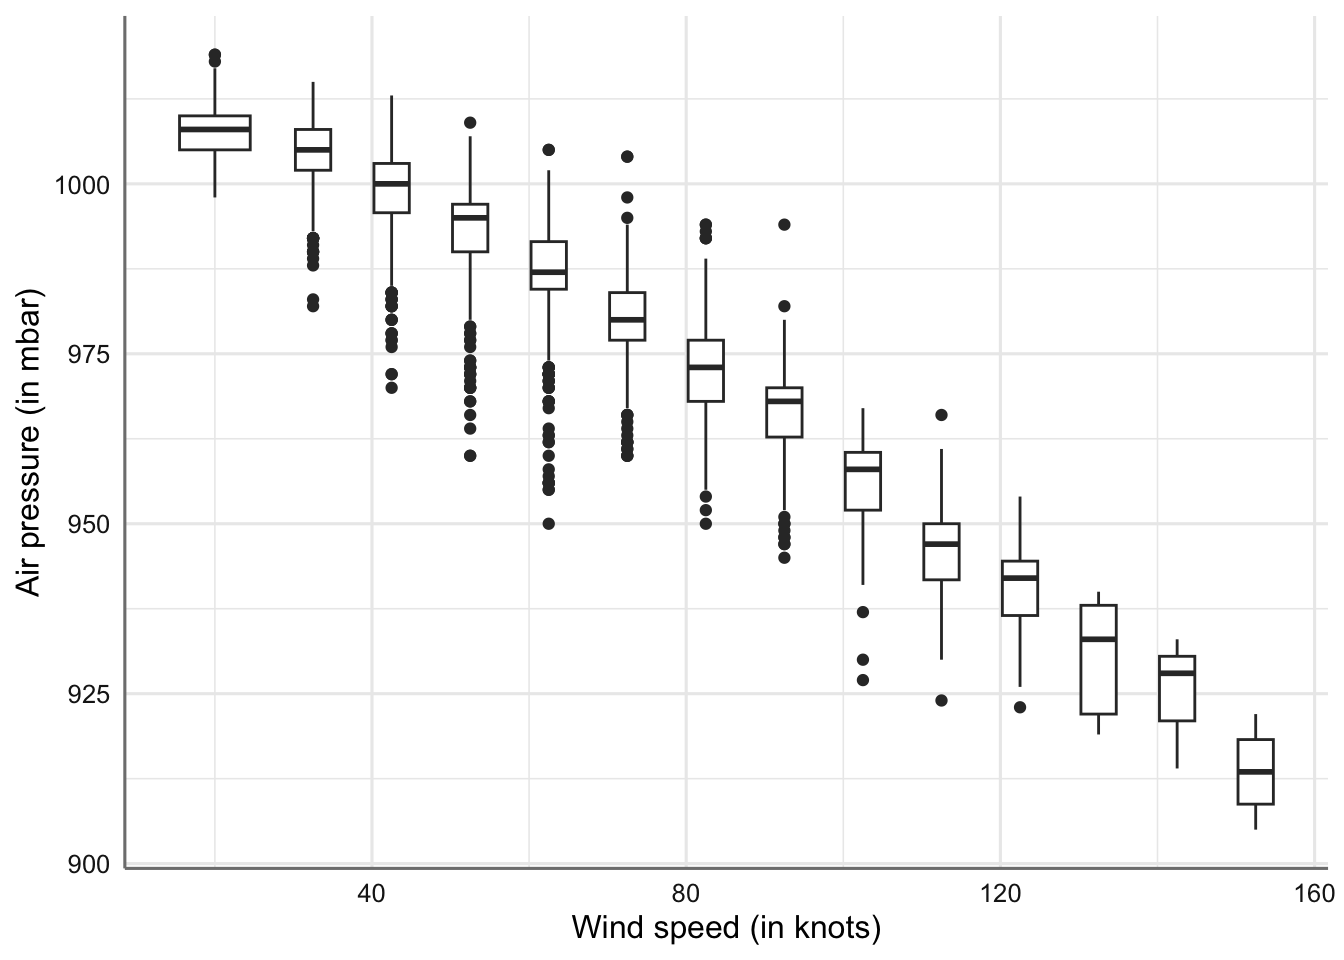
\includegraphics[width=0.95\linewidth]{02-aed_files/figure-latex/aed044-1} 

}

\caption{Gráfico de cajas discretizando la velocidad del viento vs presión atmosférica.}\label{fig:aed044}
\end{figure}

La interpretación es similar a la que se realizaba cuando trabajamos con una variable factor y otra numérica. Lo que resulta interesante es que podemos observar los intervalos con un mayor volumen de valores extremos o anómalos (valores de viento entre 30 y 90 mph).

\hypertarget{anuxe1lisis-descriptivo-avanzado}{%
\section{Análisis Descriptivo avanzado}\label{anuxe1lisis-descriptivo-avanzado}}

En esta unidad se amplían los procedimientos de análisis descriptivos vistos en el tema anterior para estudiar una o dos variables de tipo numérico o categórico al caso de más de dos variables de este tipo. No se hace un barrido a cualquier situación que pueda aparecer sino que se pretende mostrar los casos más habituales. Dichos casos son:

\begin{itemize}
\tightlist
\item
  Tres variables categóricas.
\item
  Dos variables categóricas y una variable numérica.
\item
  Una variable categórica y dos variables numéricas.
\item
  Dos variables categóricas y dos variables numéricas.
\item
  Tres variables categóricas y dos variables numéricas.
\end{itemize}

De nuevo utilizaremos el conjunto de datos \texttt{storms} de la librería \texttt{nasaweather}.

\hypertarget{tres-factores}{%
\subsection{Tres factores}\label{tres-factores}}

Los procedimientos numéricos se restringen en este caso a la obtención de la tabla de frecuencias conjunta de las tres variables, mientras que los gráficos se basan en gráficos matriciales donde se consideran gráficos de barras.

A modo de ejemplo vamos a realizar el análisis conjunto de las variables \texttt{year\_f}, \texttt{month\_f} y \texttt{type}. Para poder realizar estos análisis utilizamos la función \texttt{mytable} de la librería \texttt{moonBook}. Para conocer todas las caracter´siticas de esta función se recomienda ver la ayuda \texttt{help(mytable)}. EL problema principal con esta función es que si el número de nivles de los factores es demasiado grande resulta muy complicado visualizar todos los resultados en una única página. De hecho solo se pueden visulaizar resulatdos si el número de niveles del factor es 5 como máximo. Para poder ver los resultados en esta situación procedemos reando un conjunto de datos para cada tipo de tormenta. En este caso seleccionamos los meses centrales y los últimos cinco años para poder visualizar los resultados.

\#\texttt{\{r\ aed045,error=FALSE,warning=FALSE,message=FALSE\}\ \#stormTD\ \textless{}-\ dplyr::filter(storm\ ,\ month\ \%in\%\ c(7,8,9,10,11),\ \ \#\ \ \ \ \ \ \ \ \ \ \ \ \ \ \ \ \ \ \ \ \ \ \ \ \ year\ \%in\%\ c(1996,1997,1998,1999,2000))\ \#mytable(year\_f\ +\ type\ \textasciitilde{}\ month\_f,\ data\ =\ stormTD)\ \#}

Para realizar le gráfico combinado de las tres variables categóricas utilizamos un gráfico matricial con dos factores y representamos dentro de cada combinación el gráfico de barras de la otra variable.

\begin{Shaded}
\begin{Highlighting}[]
\NormalTok{ords }\OtherTok{\textless{}{-}} \FunctionTok{c}\NormalTok{(}\StringTok{"Tropical Depression"}\NormalTok{, }\StringTok{"Extratropical"}\NormalTok{, }\StringTok{"Tropical Storm"}\NormalTok{, }\StringTok{"Hurricane"}\NormalTok{)}
\FunctionTok{ggplot}\NormalTok{(storm, }\FunctionTok{aes}\NormalTok{(}\AttributeTok{x =}\NormalTok{ type))  }\SpecialCharTok{+}
  \FunctionTok{geom\_bar}\NormalTok{() }\SpecialCharTok{+} 
  \FunctionTok{scale\_x\_discrete}\NormalTok{(}\AttributeTok{limits =}\NormalTok{ ords) }\SpecialCharTok{+}
  \FunctionTok{xlab}\NormalTok{(}\StringTok{"Storm category"}\NormalTok{) }\SpecialCharTok{+}
  \FunctionTok{ylab}\NormalTok{(}\StringTok{"Frequency"}\NormalTok{) }\SpecialCharTok{+}
  \FunctionTok{facet\_grid}\NormalTok{(year\_f }\SpecialCharTok{\textasciitilde{}}\NormalTok{ month\_f)}\SpecialCharTok{+}
  \FunctionTok{theme}\NormalTok{(}\AttributeTok{axis.text.x =} \FunctionTok{element\_text}\NormalTok{(}\AttributeTok{angle =} \DecValTok{90}\NormalTok{)) }
\end{Highlighting}
\end{Shaded}

\begin{figure}

{\centering 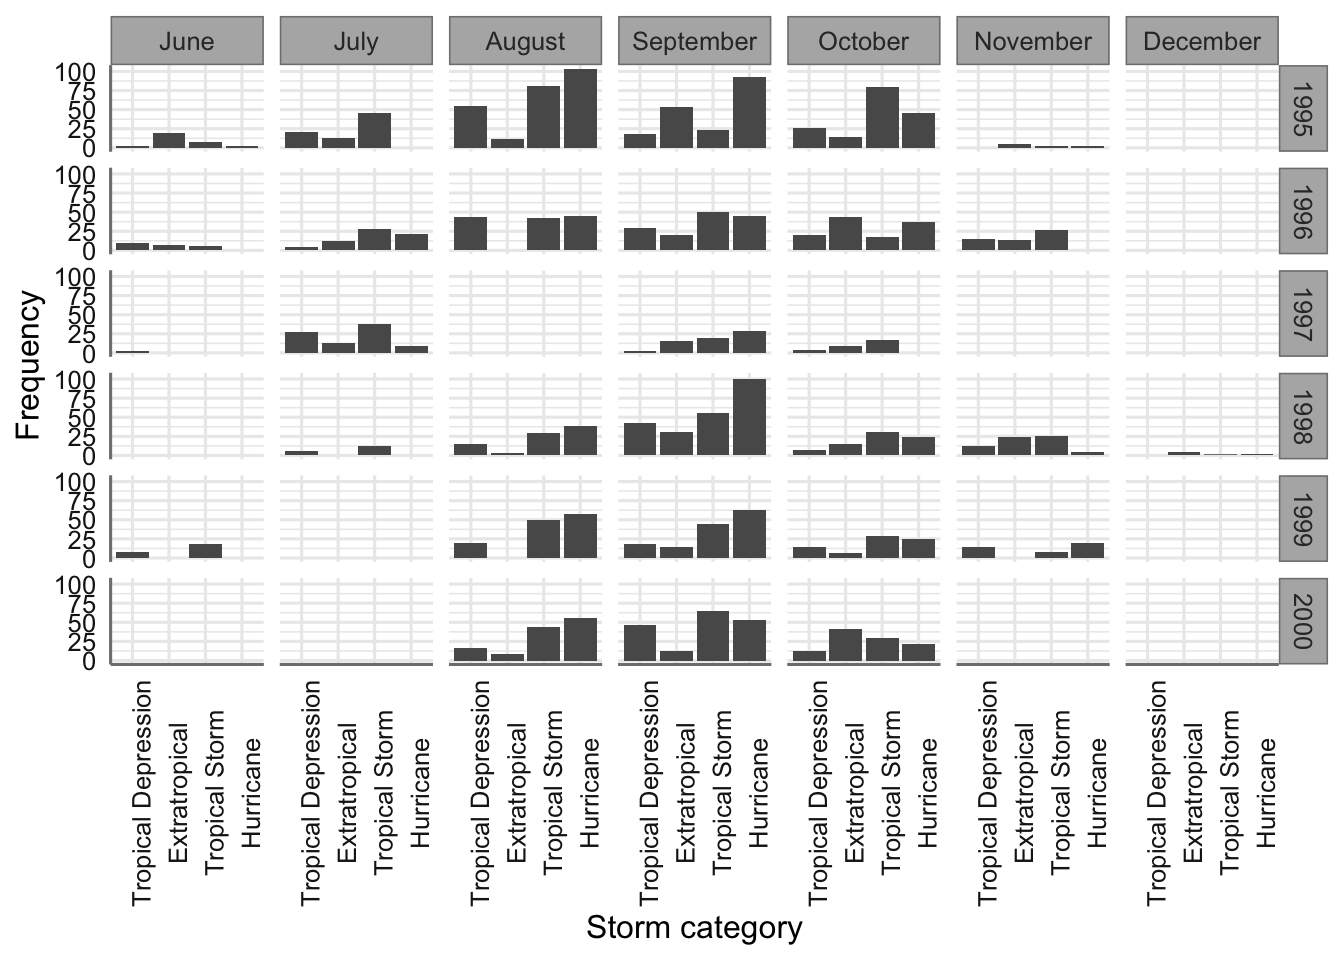
\includegraphics[width=0.95\linewidth]{02-aed_files/figure-latex/aed046-1} 

}

\caption{Gráfico de barras para tipo de tormenta para los diferentes meses y años.}\label{fig:aed046}
\end{figure}

¿Qué conclusiones podemos extraer de estos resultados? El gráfico resulta revelador, ya que se aprecian de forma directa las combinaciones de año - mes en al que no hay datos, y en aquellas donde si los hay se puede ver claramente cual es el tipo de tormenta más predominante.

Dado que la mayoría de los datos se producen entre los meses de agosto y octubre vamos a filtrar los datos para estudiar esas combinaciones únicamente.

\begin{Shaded}
\begin{Highlighting}[]
\NormalTok{storm\_meses }\OtherTok{\textless{}{-}}\NormalTok{ storm }\SpecialCharTok{\%\textgreater{}\%}
  \FunctionTok{filter}\NormalTok{(month\_f }\SpecialCharTok{==} \FunctionTok{c}\NormalTok{(}\StringTok{"August"}\NormalTok{,}\StringTok{"September"}\NormalTok{,}\StringTok{"October"}\NormalTok{))}
\NormalTok{ords }\OtherTok{\textless{}{-}} \FunctionTok{c}\NormalTok{(}\StringTok{"Tropical Depression"}\NormalTok{, }\StringTok{"Extratropical"}\NormalTok{, }\StringTok{"Tropical Storm"}\NormalTok{, }\StringTok{"Hurricane"}\NormalTok{)}
\FunctionTok{ggplot}\NormalTok{(storm\_meses, }\FunctionTok{aes}\NormalTok{(}\AttributeTok{x =}\NormalTok{ type))  }\SpecialCharTok{+}
  \FunctionTok{geom\_bar}\NormalTok{() }\SpecialCharTok{+} 
  \FunctionTok{scale\_x\_discrete}\NormalTok{(}\AttributeTok{limits =}\NormalTok{ ords) }\SpecialCharTok{+}
  \FunctionTok{xlab}\NormalTok{(}\StringTok{"Storm category"}\NormalTok{) }\SpecialCharTok{+}
  \FunctionTok{ylab}\NormalTok{(}\StringTok{"Frequency"}\NormalTok{) }\SpecialCharTok{+}
  \FunctionTok{facet\_grid}\NormalTok{(year\_f }\SpecialCharTok{\textasciitilde{}}\NormalTok{ month\_f) }\SpecialCharTok{+}
  \FunctionTok{theme}\NormalTok{(}\AttributeTok{axis.text.x =} \FunctionTok{element\_text}\NormalTok{(}\AttributeTok{angle =} \DecValTok{90}\NormalTok{)) }
\end{Highlighting}
\end{Shaded}

\begin{figure}

{\centering 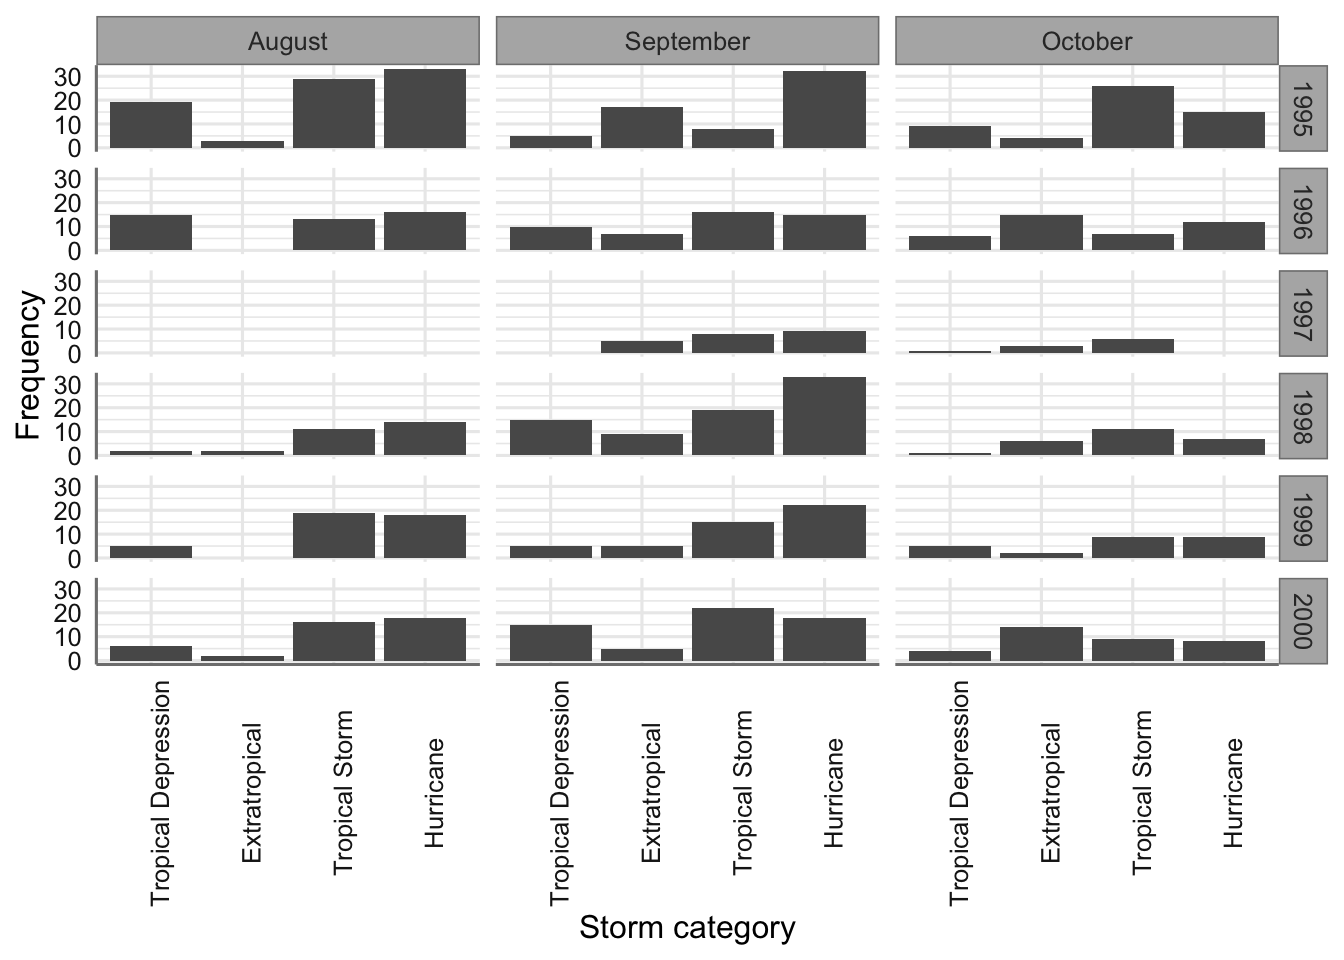
\includegraphics[width=0.95\linewidth]{02-aed_files/figure-latex/aed047-1} 

}

\caption{Gráfico de barras para tipo de tormenta para los diferentes meses y años (versión 2).}\label{fig:aed047}
\end{figure}

Este gráfico nos permite estudiar con más detalle los meses que concentran un mayor número de tormentas.

\hypertarget{dos-factores-una-numuxe9rica}{%
\subsection{Dos factores, Una numérica}\label{dos-factores-una-numuxe9rica}}

En este caso generalizamos el cálculo de medidas de localización y dispersión a esta situación, y analizamos los diferentes gráficos que podemos realizar en esta situación. Utilizamos las variables \texttt{year\_f}, \texttt{type}, y \texttt{wind}. Mostraremos solo los datos para los años 1999 y 2000.

\begin{Shaded}
\begin{Highlighting}[]
\NormalTok{stormTD }\OtherTok{\textless{}{-}}\NormalTok{ dplyr}\SpecialCharTok{::}\FunctionTok{filter}\NormalTok{(storm , year }\SpecialCharTok{\%in\%} \FunctionTok{c}\NormalTok{(}\DecValTok{1999}\NormalTok{,}\DecValTok{2000}\NormalTok{))}
\FunctionTok{mytable}\NormalTok{(year\_f }\SpecialCharTok{+}\NormalTok{ type }\SpecialCharTok{\textasciitilde{}}\NormalTok{ wind, }\AttributeTok{data =}\NormalTok{ stormTD)}
\end{Highlighting}
\end{Shaded}

\begin{verbatim}
## 
##                                          Descriptive Statistics stratified by 'year_f' and 'type'                                         
## ——————————————————————————————————————————————————————————————————————————————————————————————————————————————————————————————————————————— 
##                                       1999                                                                2000                                
##       —————————————————————————————————————————————————————————————————— —————————————————————————————————————————————————————————————————— 
##       Extratropical  Hurricane  Tropical Depression Tropical Storm   p   Extratropical  Hurricane  Tropical Depression Tropical Storm   p  
##          (N=22)       (N=164)         (N=75)           (N=150)             (N=63)       (N=130)         (N=76)           (N=138)         
## ——————————————————————————————————————————————————————————————————————————————————————————————————————————————————————————————————————————— 
##  Wind  38.9 ± 20.3  90.5 ± 20.7     27.1 ±  3.9      47.7 ±  8.1   0.000  39.7 ± 13.2  79.5 ± 14.7     27.8 ±  2.6      46.2 ±  8.5   0.000
## ———————————————————————————————————————————————————————————————————————————————————————————————————————————————————————————————————————————
\end{verbatim}

Como antes el análisis de estas tablas es más complejo que tratar de representar los datos de forma que se puedan extraer conclusiones de forma más efectiva. Empezamos con el gráfico matricial mezclado con los gráficos de densidad.

\begin{Shaded}
\begin{Highlighting}[]
\CommentTok{\# Creamos un nuevo factor ordenado de acurdo a la variable que estamos midiendo}
\NormalTok{storm}\SpecialCharTok{$}\NormalTok{type2 }\OtherTok{\textless{}{-}} \FunctionTok{reorder}\NormalTok{(storm}\SpecialCharTok{$}\NormalTok{type, storm}\SpecialCharTok{$}\NormalTok{wind)}
\CommentTok{\# Creamos el gráfico}
\FunctionTok{ggplot}\NormalTok{(storm, }\FunctionTok{aes}\NormalTok{(}\AttributeTok{x =}\NormalTok{ wind, }\AttributeTok{color =}\NormalTok{ type2))  }\SpecialCharTok{+}
  \FunctionTok{geom\_density}\NormalTok{(}\AttributeTok{bw =} \DecValTok{3}\NormalTok{) }\SpecialCharTok{+} 
  \FunctionTok{xlab}\NormalTok{(}\StringTok{"Wind speed (in knots)"}\NormalTok{) }\SpecialCharTok{+}
  \FunctionTok{ylab}\NormalTok{(}\StringTok{"Density"}\NormalTok{) }\SpecialCharTok{+}
  \FunctionTok{facet\_grid}\NormalTok{(year\_f }\SpecialCharTok{\textasciitilde{}}\NormalTok{ .)}
\end{Highlighting}
\end{Shaded}

\begin{figure}

{\centering 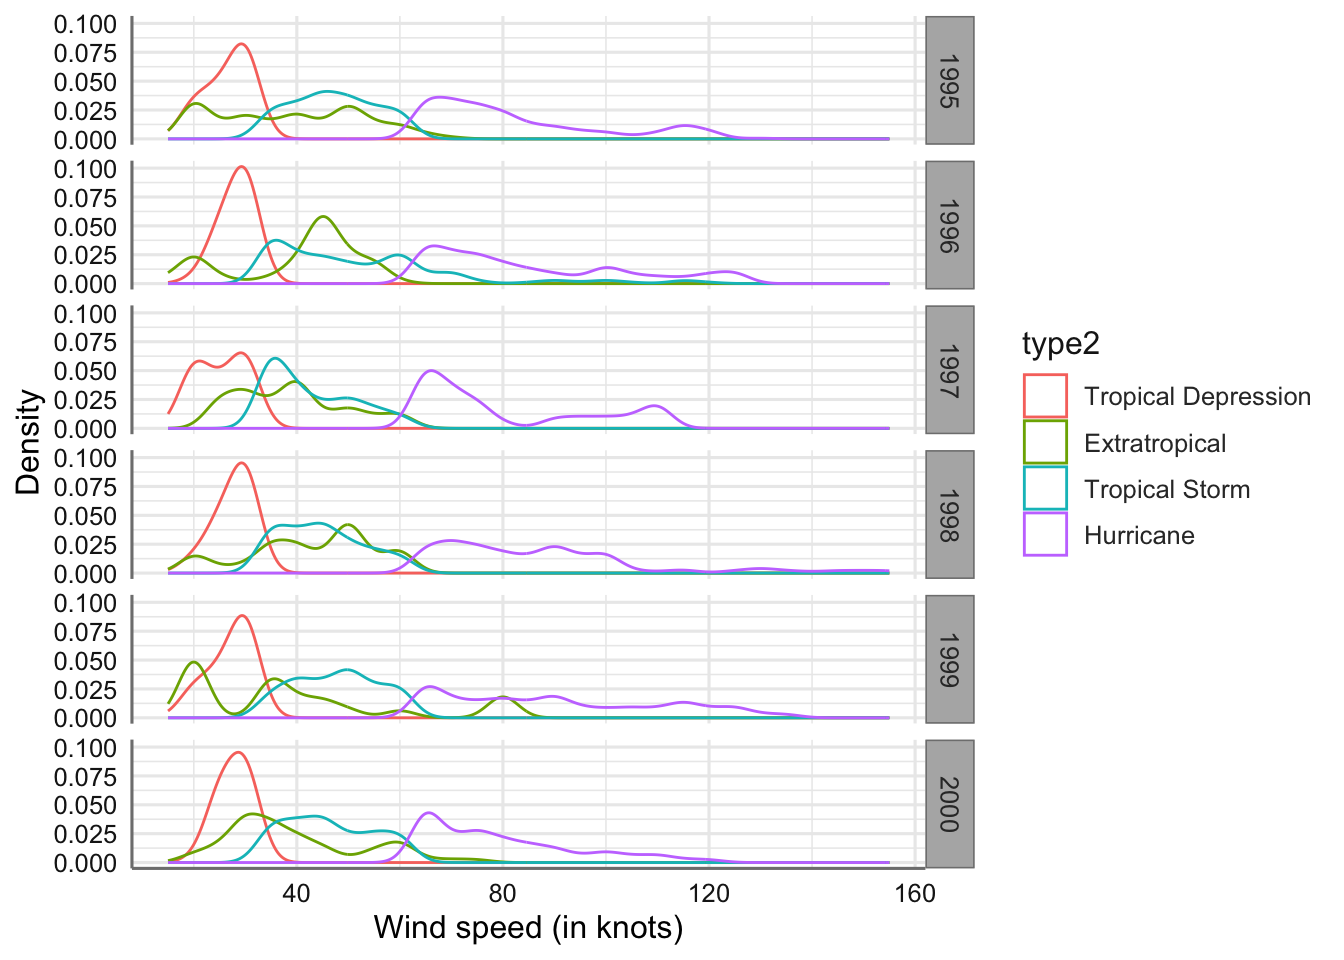
\includegraphics[width=0.95\linewidth]{02-aed_files/figure-latex/aed049-1} 

}

\caption{Gráfico de densidad de la velocidad del viento para cada tipo de tormenta y año.}\label{fig:aed049}
\end{figure}

Ahora realizamos el gráfico de cajas con una estructura similar

\begin{Shaded}
\begin{Highlighting}[]
\CommentTok{\# Creamos el gráfico}
\FunctionTok{ggplot}\NormalTok{(storm, }\FunctionTok{aes}\NormalTok{(}\AttributeTok{x =}\NormalTok{ type2, }\AttributeTok{y =}\NormalTok{ wind))  }\SpecialCharTok{+}
  \FunctionTok{geom\_boxplot}\NormalTok{() }\SpecialCharTok{+} 
  \FunctionTok{xlab}\NormalTok{(}\StringTok{"Storm category"}\NormalTok{) }\SpecialCharTok{+}
  \FunctionTok{ylab}\NormalTok{(}\StringTok{"Wind speed (in knots)"}\NormalTok{) }\SpecialCharTok{+}
  \FunctionTok{facet\_grid}\NormalTok{(. }\SpecialCharTok{\textasciitilde{}}\NormalTok{ year\_f) }\SpecialCharTok{+}
  \FunctionTok{theme}\NormalTok{(}\AttributeTok{axis.text.x =} \FunctionTok{element\_text}\NormalTok{(}\AttributeTok{angle =} \DecValTok{90}\NormalTok{))}
\end{Highlighting}
\end{Shaded}

\begin{figure}

{\centering 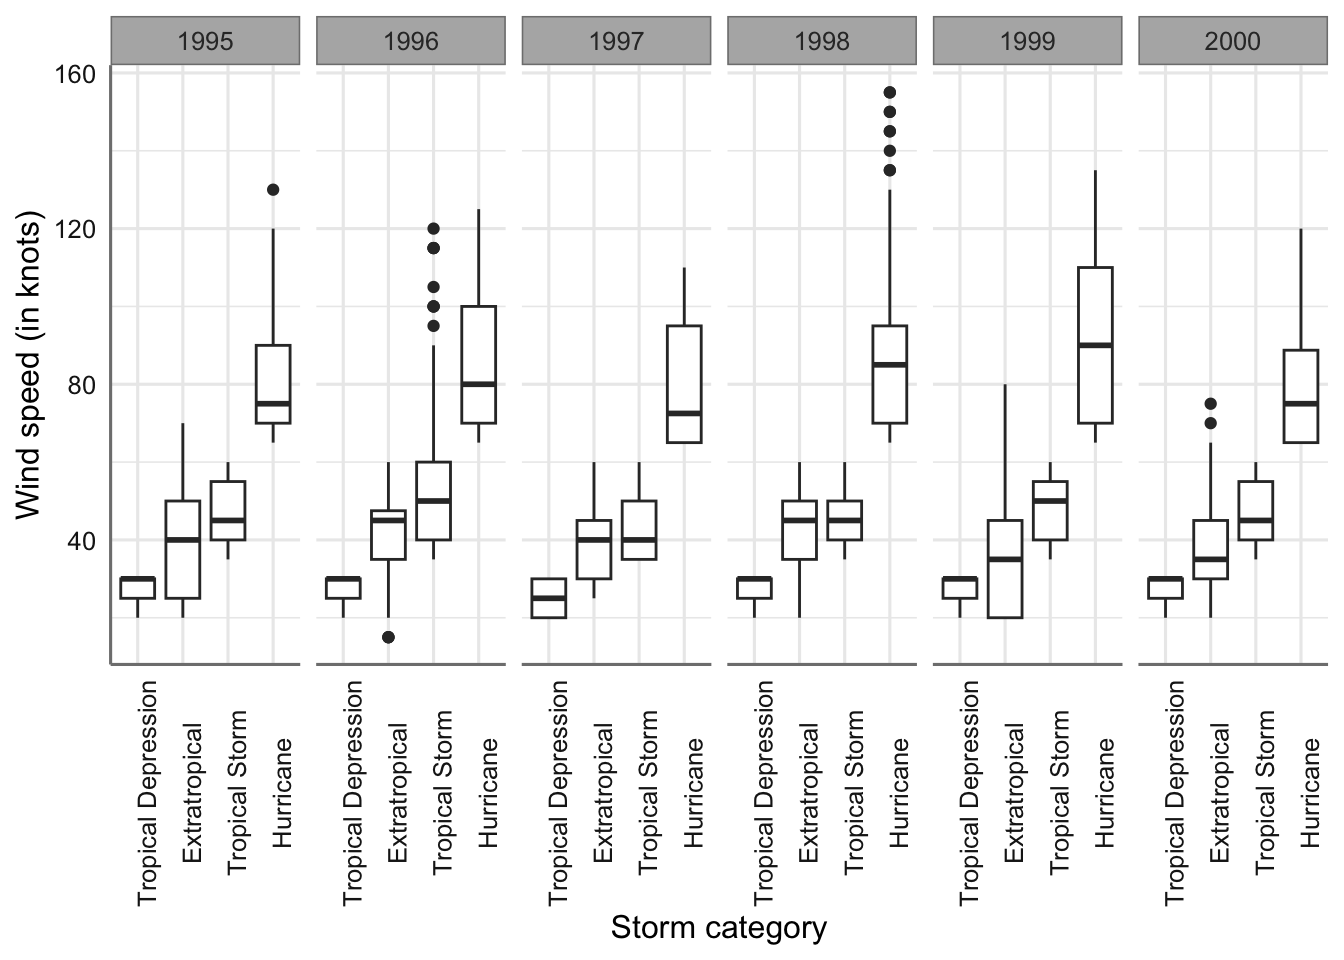
\includegraphics[width=0.95\linewidth]{02-aed_files/figure-latex/aed050-1} 

}

\caption{Gráfico de cajas de la velocidad del viento para cada tipo de tormenta y año.}\label{fig:aed050}
\end{figure}

¿Qué conclusiones podemos extraer de este gráfico?

Otra versión de este gráfico podría ser:

\begin{Shaded}
\begin{Highlighting}[]
\CommentTok{\# Creamos el gráfico}
\FunctionTok{ggplot}\NormalTok{(storm, }\FunctionTok{aes}\NormalTok{(}\AttributeTok{x =}\NormalTok{ year\_f, }\AttributeTok{y =}\NormalTok{ wind, }\AttributeTok{color =}\NormalTok{ type2))  }\SpecialCharTok{+}
  \FunctionTok{geom\_boxplot}\NormalTok{() }\SpecialCharTok{+} 
  \FunctionTok{xlab}\NormalTok{(}\StringTok{"Year"}\NormalTok{) }\SpecialCharTok{+}
  \FunctionTok{ylab}\NormalTok{(}\StringTok{"Wind speed (in knots)"}\NormalTok{) }
\end{Highlighting}
\end{Shaded}

\begin{figure}

{\centering 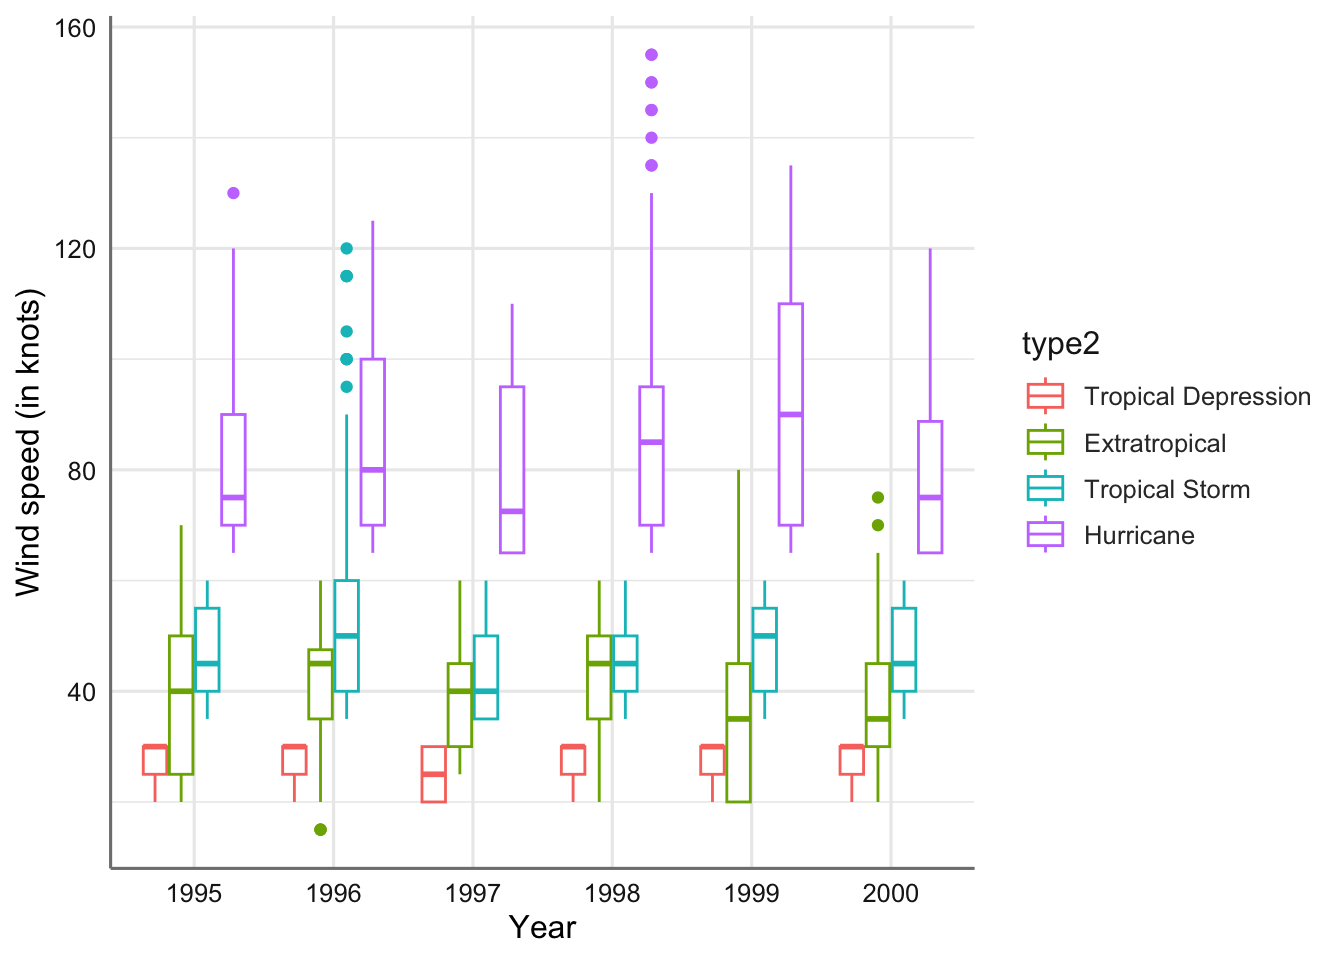
\includegraphics[width=0.95\linewidth]{02-aed_files/figure-latex/aed051-1} 

}

\caption{Gráfico de cajas de la velocidad del viento para cada tipo de tormenta y año (versión 2).}\label{fig:aed051}
\end{figure}

\hypertarget{un-factor-dos-numuxe9ricas}{%
\subsection{Un factor, Dos numéricas}\label{un-factor-dos-numuxe9ricas}}

En este caso generalizamos el análisis de correlación y el gráfico de dispersión con la inclusión del factor. Consideramos las variables \texttt{type}, \texttt{wind} y \texttt{pressure}. En primer lugar realizamos el estudio descriptivo numérico.

\begin{Shaded}
\begin{Highlighting}[]
\NormalTok{storm }\SpecialCharTok{\%\textgreater{}\%} 
  \FunctionTok{group\_by}\NormalTok{(type) }\SpecialCharTok{\%\textgreater{}\%} \CommentTok{\# Segmentamos por tipo de tormenta}
  \FunctionTok{summarise}\NormalTok{(}\AttributeTok{cor =} \FunctionTok{cor}\NormalTok{(wind,pressure)) }\CommentTok{\# Obtenemos coeficientes de correlación}
\end{Highlighting}
\end{Shaded}

\begin{verbatim}
## # A tibble: 4 x 2
##   type                   cor
##   <fct>                <dbl>
## 1 Extratropical       -0.816
## 2 Hurricane           -0.914
## 3 Tropical Depression -0.157
## 4 Tropical Storm      -0.819
\end{verbatim}

El resultado muestra gran asociación entre la velocidad del viento y la presión atmosférica en todas la categorías salvo para las Depresiones tropicales.

Veamos ahora el gráfico de dispersión conjunto. En primer lugar realizamos un único gráfico marcando con colores los tipos de tormenta

\begin{Shaded}
\begin{Highlighting}[]
\FunctionTok{ggplot}\NormalTok{(storm, }\FunctionTok{aes}\NormalTok{(}\AttributeTok{x =}\NormalTok{ wind, }\AttributeTok{y =}\NormalTok{ pressure, }\AttributeTok{color =}\NormalTok{ type )) }\SpecialCharTok{+} 
  \FunctionTok{geom\_point}\NormalTok{() }\SpecialCharTok{+} 
  \FunctionTok{labs}\NormalTok{(}\AttributeTok{x =} \StringTok{"Wind speed (in knots)"}\NormalTok{, }\AttributeTok{y =} \StringTok{"Air pressure (in mbar)"}\NormalTok{)}
\end{Highlighting}
\end{Shaded}

\begin{figure}

{\centering 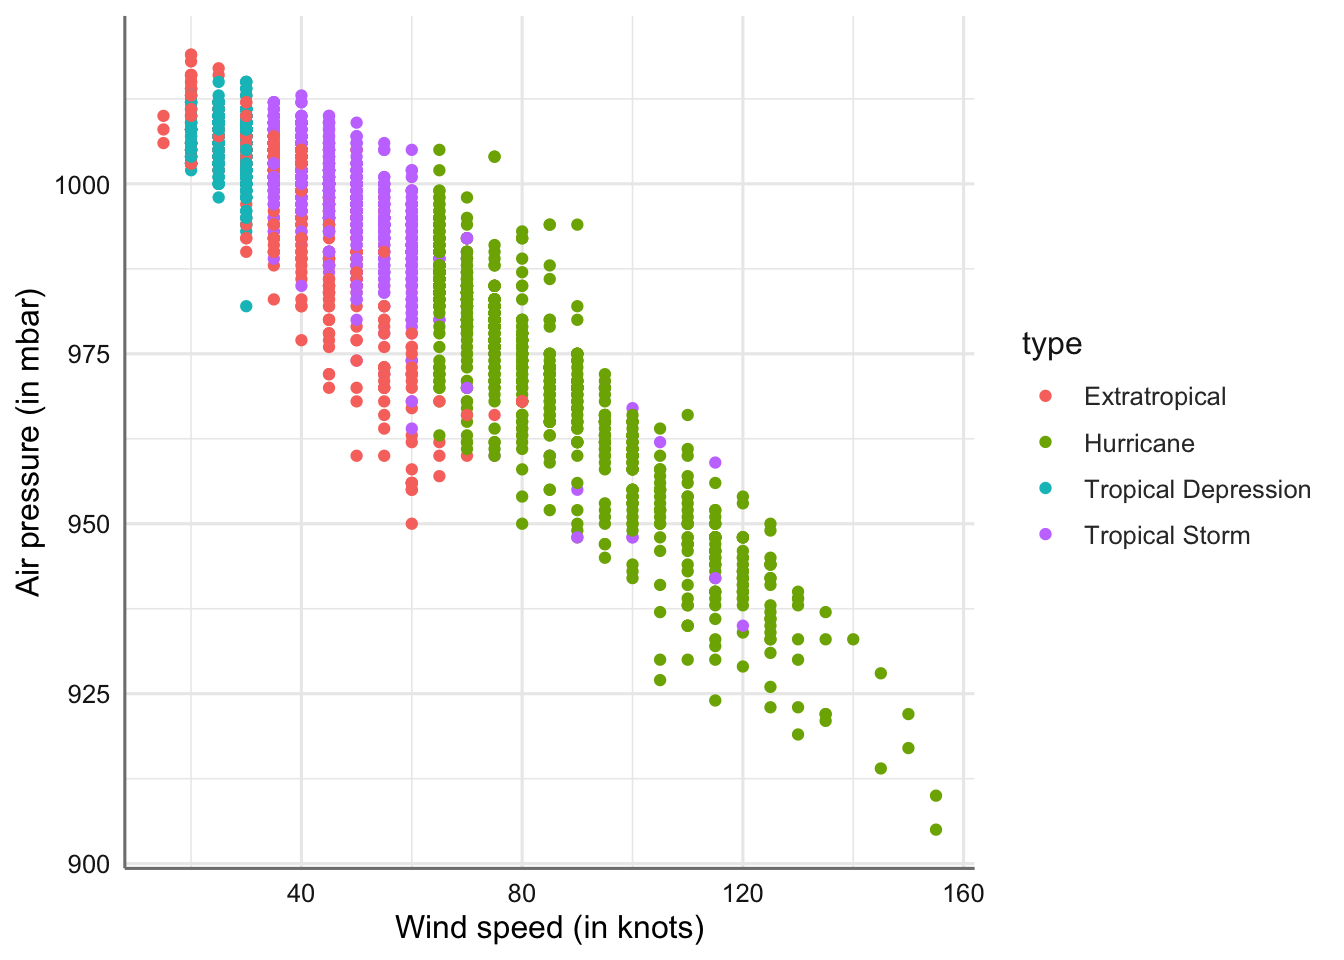
\includegraphics[width=0.95\linewidth]{02-aed_files/figure-latex/aed053-1} 

}

\caption{Gráfico de dispersion de presión vs velocidad para cada tipo de tormenta.}\label{fig:aed053}
\end{figure}

Podemos ver como cada punto viene identificado según el tipo de tormenta. Los huracanes en la parte inferior donde se dan las relaciones entre velocidades del viento más altas y presiones atmosféricas más bajas. ¿Qué más podemos decir?

Podemos distinguir cada grupo introduciendo un gráfico matricial

\begin{Shaded}
\begin{Highlighting}[]
\CommentTok{\# Creamos el gráfico}
\FunctionTok{ggplot}\NormalTok{(storm, }\FunctionTok{aes}\NormalTok{(}\AttributeTok{x =}\NormalTok{ wind, }\AttributeTok{y =}\NormalTok{ pressure))  }\SpecialCharTok{+}
  \FunctionTok{geom\_point}\NormalTok{() }\SpecialCharTok{+} 
  \FunctionTok{xlab}\NormalTok{(}\StringTok{"Wind speed (in knots)"}\NormalTok{) }\SpecialCharTok{+}
  \FunctionTok{ylab}\NormalTok{(}\StringTok{"Air pressure (in mbar)"}\NormalTok{) }\SpecialCharTok{+}
  \FunctionTok{facet\_grid}\NormalTok{(. }\SpecialCharTok{\textasciitilde{}}\NormalTok{ type2) }
\end{Highlighting}
\end{Shaded}

\begin{figure}

{\centering 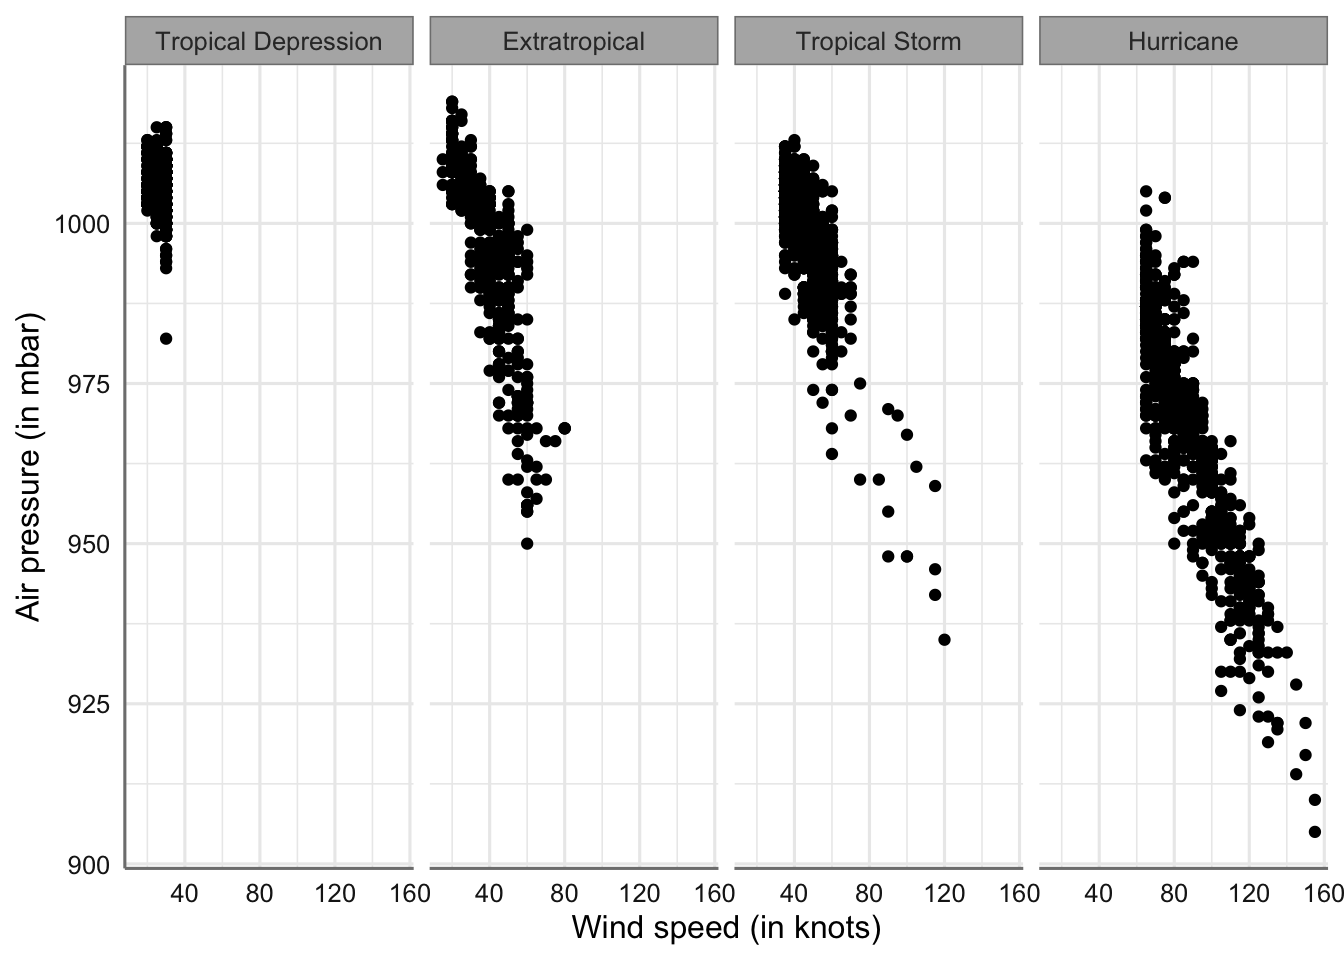
\includegraphics[width=0.95\linewidth]{02-aed_files/figure-latex/aed054-1} 

}

\caption{Gráfico de dispersion de presión vs velocidad para cada tipo de tormenta.}\label{fig:aed054}
\end{figure}

En este gráfico se aprecia mejor el comportamiento de ambas variables en cada uno de los niveles del factor. Salvo en las depresiones tropicales donde no se aprecia asociación, en el resto de niveles se aprecia un relación de orden inverso. Lo que si podemos ver es que hay observaciones en algunas categorías que podrían corresponder a otras. En la categoría de tormentas tropicales tenemos combinaciones de velocidad y presión que parecen corresponder más a un huracán que a una tormenta tropical. Esto puede ser debido al protocolo de clasificación establecido o a la propia evolución de las tormentas.

\hypertarget{dos-factores-dos-numuxe9ricas}{%
\subsection{Dos factores, Dos numéricas}\label{dos-factores-dos-numuxe9ricas}}

Este caso es una generalización directa del caso anterior, ya que únicamente debemos añadir una nueva variable categórica. Consideramos las variables \texttt{type}, \texttt{year\_f}, \texttt{wind} y \texttt{pressure}. Comenzamos con el análisis numérico:

\begin{Shaded}
\begin{Highlighting}[]
\NormalTok{tabla\_cor }\OtherTok{\textless{}{-}}\NormalTok{ storm }\SpecialCharTok{\%\textgreater{}\%} 
  \FunctionTok{group\_by}\NormalTok{(year\_f,type) }\SpecialCharTok{\%\textgreater{}\%} 
  \FunctionTok{summarise}\NormalTok{(}\AttributeTok{cor =} \FunctionTok{cor}\NormalTok{(wind,pressure))}
\CommentTok{\# Visulaizamos la tabla de resultados de forma óptima}
\NormalTok{tabla\_resumen }\OtherTok{\textless{}{-}}\NormalTok{ dplyr}\SpecialCharTok{::}\FunctionTok{select}\NormalTok{(tabla\_cor,year\_f,type,cor)}
\CommentTok{\# Arreglamos la tabla para una mejor visualización}
\FunctionTok{spread}\NormalTok{(tabla\_resumen, }\AttributeTok{key =}\NormalTok{ type, }\AttributeTok{value =}\NormalTok{ cor)}
\end{Highlighting}
\end{Shaded}

\begin{verbatim}
## # A tibble: 6 x 5
## # Groups:   year_f [6]
##   year_f Extratropical Hurricane `Tropical Depression` `Tropical Storm`
##   <fct>          <dbl>     <dbl>                 <dbl>            <dbl>
## 1 1995          -0.848    -0.885                 0.113           -0.731
## 2 1996          -0.826    -0.941                -0.290           -0.917
## 3 1997          -0.781    -0.973                -0.455           -0.748
## 4 1998          -0.726    -0.947                -0.271           -0.613
## 5 1999          -0.961    -0.916                -0.170           -0.661
## 6 2000          -0.915    -0.940                -0.127           -0.791
\end{verbatim}

En esta tabla aparecen representados los coeficientes de correlación entre viento y presión para las diferentes combinaciones de niveles de las variables tipo y año. Se aprecian valores muy bajos en todas las combinaciones de la depresión tropical, mientras que en el resto hay asociaciones que pueden resultar interesantes de estudiar posteriormente. En el caso de los huracanes esas asociaciones son muy fuertes ya que muestran valores muy próximos a -1.

En cuanto a los procedimientos gráficos optamos por una combinación de los gráficos que utilizamos en la sección anterior. Representamos el gráfico de dispersión coloreando por tipo de tormenta, y usamos un diagrama matricial por año.

\begin{Shaded}
\begin{Highlighting}[]
\CommentTok{\# Creamos el gráfico}
\FunctionTok{ggplot}\NormalTok{(storm, }\FunctionTok{aes}\NormalTok{(}\AttributeTok{x =}\NormalTok{ wind, }\AttributeTok{y =}\NormalTok{ pressure, }\AttributeTok{color =}\NormalTok{ type2))  }\SpecialCharTok{+}
  \FunctionTok{geom\_point}\NormalTok{() }\SpecialCharTok{+} 
  \FunctionTok{xlab}\NormalTok{(}\StringTok{"Wind speed (in knots)"}\NormalTok{) }\SpecialCharTok{+}
  \FunctionTok{ylab}\NormalTok{(}\StringTok{"Air pressure (in mbar)"}\NormalTok{) }\SpecialCharTok{+}
  \FunctionTok{facet\_grid}\NormalTok{(. }\SpecialCharTok{\textasciitilde{}}\NormalTok{ year\_f) }
\end{Highlighting}
\end{Shaded}

\begin{figure}

{\centering 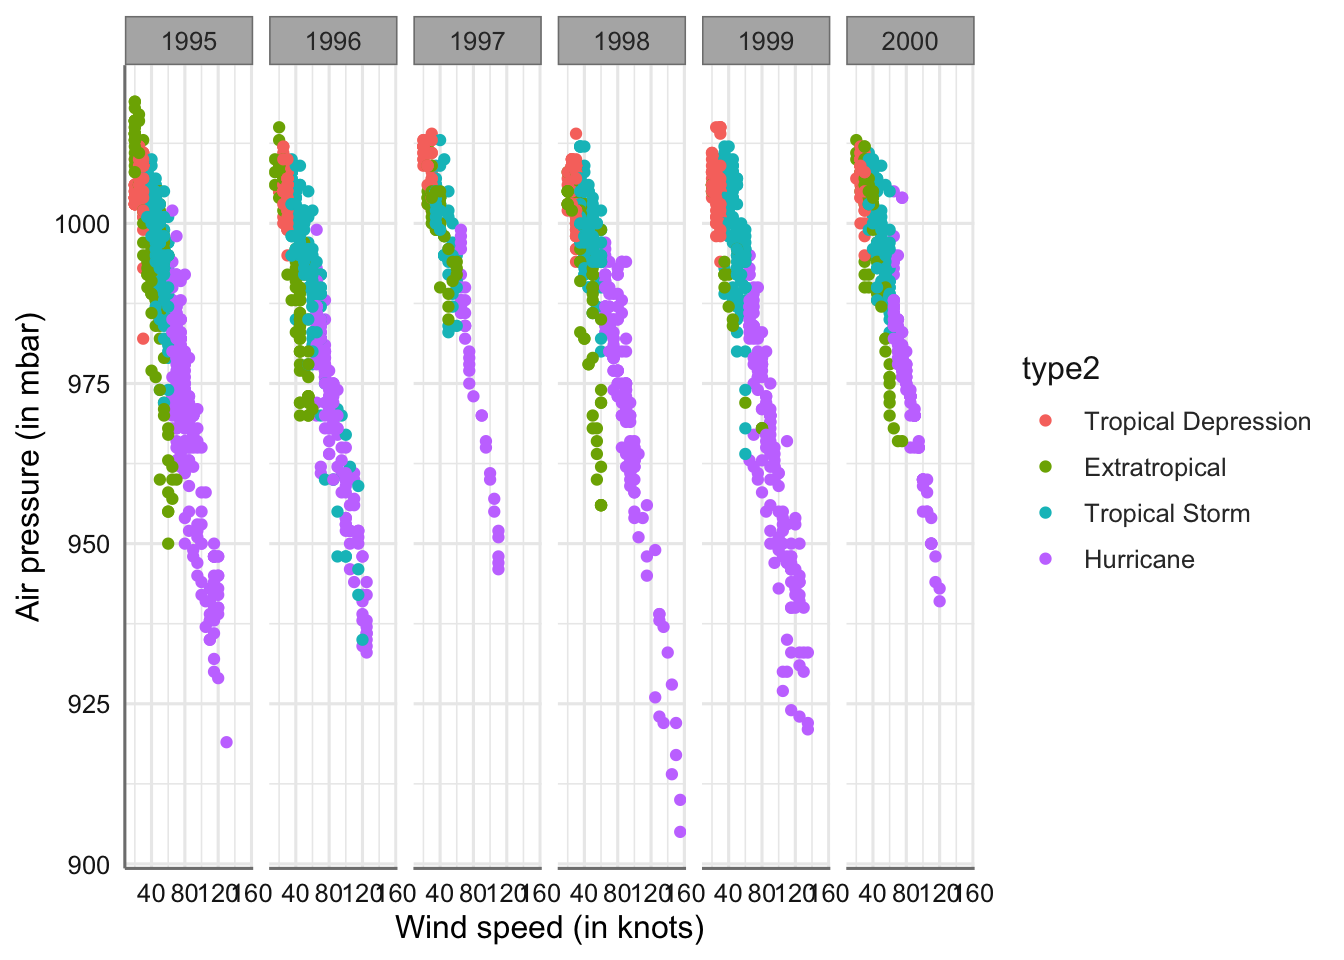
\includegraphics[width=0.95\linewidth]{02-aed_files/figure-latex/aed056-1} 

}

\caption{Gráfico de dispersion de presión vs velocidad para cada tipo de tormenta y año.}\label{fig:aed056}
\end{figure}

En todos los años se observa un comportamiento similar del resto de variables, indicando que el año no es una factor que pueda ser considerado como relevante. Si utilizamos la variable mes en su lugar el gráfico resultante es:

\begin{Shaded}
\begin{Highlighting}[]
\CommentTok{\# Creamos el gráfico}
\FunctionTok{ggplot}\NormalTok{(storm, }\FunctionTok{aes}\NormalTok{(}\AttributeTok{x =}\NormalTok{ wind, }\AttributeTok{y =}\NormalTok{ pressure, }\AttributeTok{color =}\NormalTok{ type2))  }\SpecialCharTok{+}
  \FunctionTok{geom\_point}\NormalTok{() }\SpecialCharTok{+} 
  \FunctionTok{xlab}\NormalTok{(}\StringTok{"Wind speed (in knots)"}\NormalTok{) }\SpecialCharTok{+}
  \FunctionTok{ylab}\NormalTok{(}\StringTok{"Air pressure (in mbar)"}\NormalTok{) }\SpecialCharTok{+}
  \FunctionTok{facet\_grid}\NormalTok{(. }\SpecialCharTok{\textasciitilde{}}\NormalTok{ month\_f) }\SpecialCharTok{+}
  \FunctionTok{theme}\NormalTok{(}\AttributeTok{axis.text.x =} \FunctionTok{element\_text}\NormalTok{(}\AttributeTok{angle =} \DecValTok{90}\NormalTok{))}
\end{Highlighting}
\end{Shaded}

\begin{figure}

{\centering 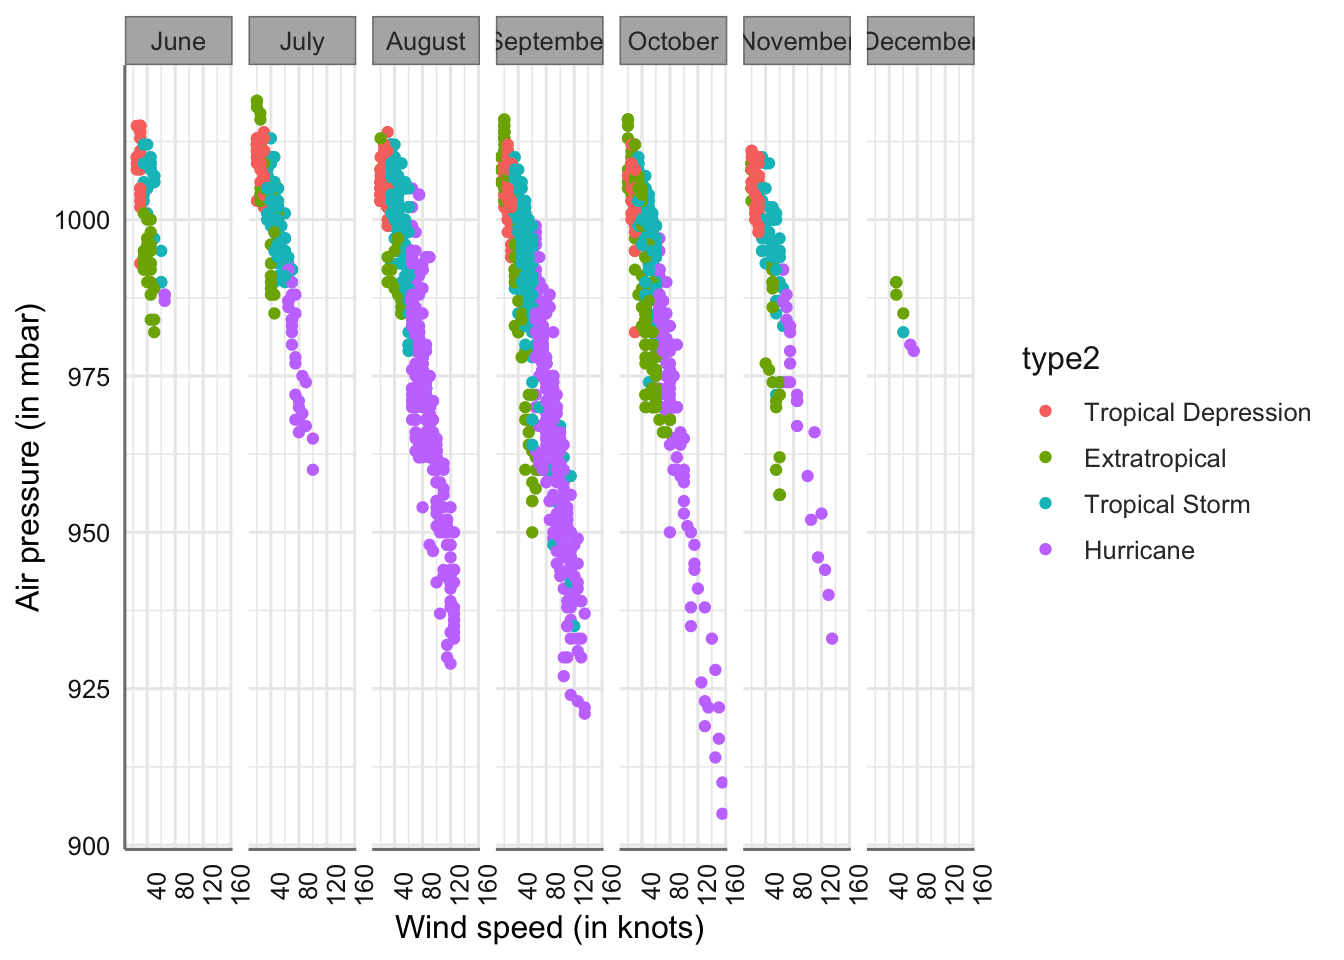
\includegraphics[width=0.95\linewidth]{02-aed_files/figure-latex/aed057-1} 

}

\caption{Gráfico de dispersion de presión vs velocidad para cada tipo de tormenta y mes}\label{fig:aed057}
\end{figure}

En este caso el comportamiento de los meses no es tan parecido. Si bien es cierto que en todas las combinaciones se aprecia una tendencia negativa (sube viento - baja presión), también se puede ver que los huracanes aparecen mayoritariamente en los meses de agosto a octubre. ¿Qué otra información podemos extraer de este gráfico?

\hypertarget{tres-factores-dos-numuxe9ricas}{%
\subsection{Tres factores, Dos numéricas}\label{tres-factores-dos-numuxe9ricas}}

Es una generalización directa de los dos casos anteriores. Se presenta únicamente el código para obtener los resultados. Añadimos la variable \texttt{month\_f} a las del caso anterior.

\begin{Shaded}
\begin{Highlighting}[]
\NormalTok{tabla\_cor }\OtherTok{\textless{}{-}}\NormalTok{ storm }\SpecialCharTok{\%\textgreater{}\%} 
  \FunctionTok{group\_by}\NormalTok{(year\_f,month\_f,type) }\SpecialCharTok{\%\textgreater{}\%} 
  \FunctionTok{summarise}\NormalTok{(}\AttributeTok{cor =} \FunctionTok{cor}\NormalTok{(wind,pressure))}
\CommentTok{\# Visulaizamos la tabla de resultados de forma óptima}
\NormalTok{tabla\_resumen }\OtherTok{\textless{}{-}}\NormalTok{ dplyr}\SpecialCharTok{::}\FunctionTok{select}\NormalTok{(tabla\_cor,year\_f,month\_f,type,cor)}
\FunctionTok{spread}\NormalTok{(tabla\_resumen, }\AttributeTok{key =}\NormalTok{ type, }\AttributeTok{value =}\NormalTok{ cor)}
\end{Highlighting}
\end{Shaded}

\begin{verbatim}
## # A tibble: 30 x 6
## # Groups:   year_f, month_f [30]
##    year_f month_f   Extratropical Hurricane `Tropical Depression` `Tropical Storm`
##    <fct>  <fct>             <dbl>     <dbl>                 <dbl>            <dbl>
##  1 1995   June             -0.688    NA                   NA                -0.849
##  2 1995   July             -0.816    NA                    0.121            -0.701
##  3 1995   August           -0.926    -0.750                0.294            -0.805
##  4 1995   September        -0.881    -0.931               -0.203            -0.937
##  5 1995   October          -0.954    -0.918               -0.0585           -0.727
##  6 1995   November         -0.968    NA                   NA                 1    
##  7 1996   June             -0.591    NA                   -0.828             0    
##  8 1996   July             -0.165    -0.779               -0.612            -0.955
##  9 1996   August           NA        -0.976               -0.0301           -0.830
## 10 1996   September        -0.887    -0.852                0.0622           -0.927
## # ... with 20 more rows
\end{verbatim}

¿Qué podemos decir de los resultados obtenidos?

Veamos ahora el gráfico matricial. Seleccionamos los meses de agosto a octubre para poder visualizarlo mejor.

\begin{Shaded}
\begin{Highlighting}[]
\NormalTok{storm\_meses }\OtherTok{\textless{}{-}}\NormalTok{ storm }\SpecialCharTok{\%\textgreater{}\%}
  \FunctionTok{filter}\NormalTok{(month\_f }\SpecialCharTok{==} \FunctionTok{c}\NormalTok{(}\StringTok{"August"}\NormalTok{,}\StringTok{"September"}\NormalTok{,}\StringTok{"October"}\NormalTok{))}
\CommentTok{\# Creamos un nuevo factor ordenado de acurdo a la variable que estamos midiendo}
\NormalTok{storm\_meses}\SpecialCharTok{$}\NormalTok{type2 }\OtherTok{\textless{}{-}} \FunctionTok{reorder}\NormalTok{(storm\_meses}\SpecialCharTok{$}\NormalTok{type, storm\_meses}\SpecialCharTok{$}\NormalTok{wind)}
\CommentTok{\# Creamos el gráfico}
\FunctionTok{ggplot}\NormalTok{(storm\_meses, }\FunctionTok{aes}\NormalTok{(}\AttributeTok{x =}\NormalTok{ wind, }\AttributeTok{y =}\NormalTok{ pressure, }\AttributeTok{color =}\NormalTok{ type2))  }\SpecialCharTok{+}
  \FunctionTok{geom\_point}\NormalTok{() }\SpecialCharTok{+} 
  \FunctionTok{xlab}\NormalTok{(}\StringTok{"Wind speed (in knots)"}\NormalTok{) }\SpecialCharTok{+}
  \FunctionTok{ylab}\NormalTok{(}\StringTok{"Air pressure (in mbar)"}\NormalTok{) }\SpecialCharTok{+}
  \FunctionTok{facet\_grid}\NormalTok{(year\_f }\SpecialCharTok{\textasciitilde{}}\NormalTok{ month\_f) }\SpecialCharTok{+}
  \FunctionTok{theme}\NormalTok{(}\AttributeTok{axis.text.x =} \FunctionTok{element\_text}\NormalTok{(}\AttributeTok{angle =} \DecValTok{90}\NormalTok{))}
\end{Highlighting}
\end{Shaded}

\begin{figure}

{\centering 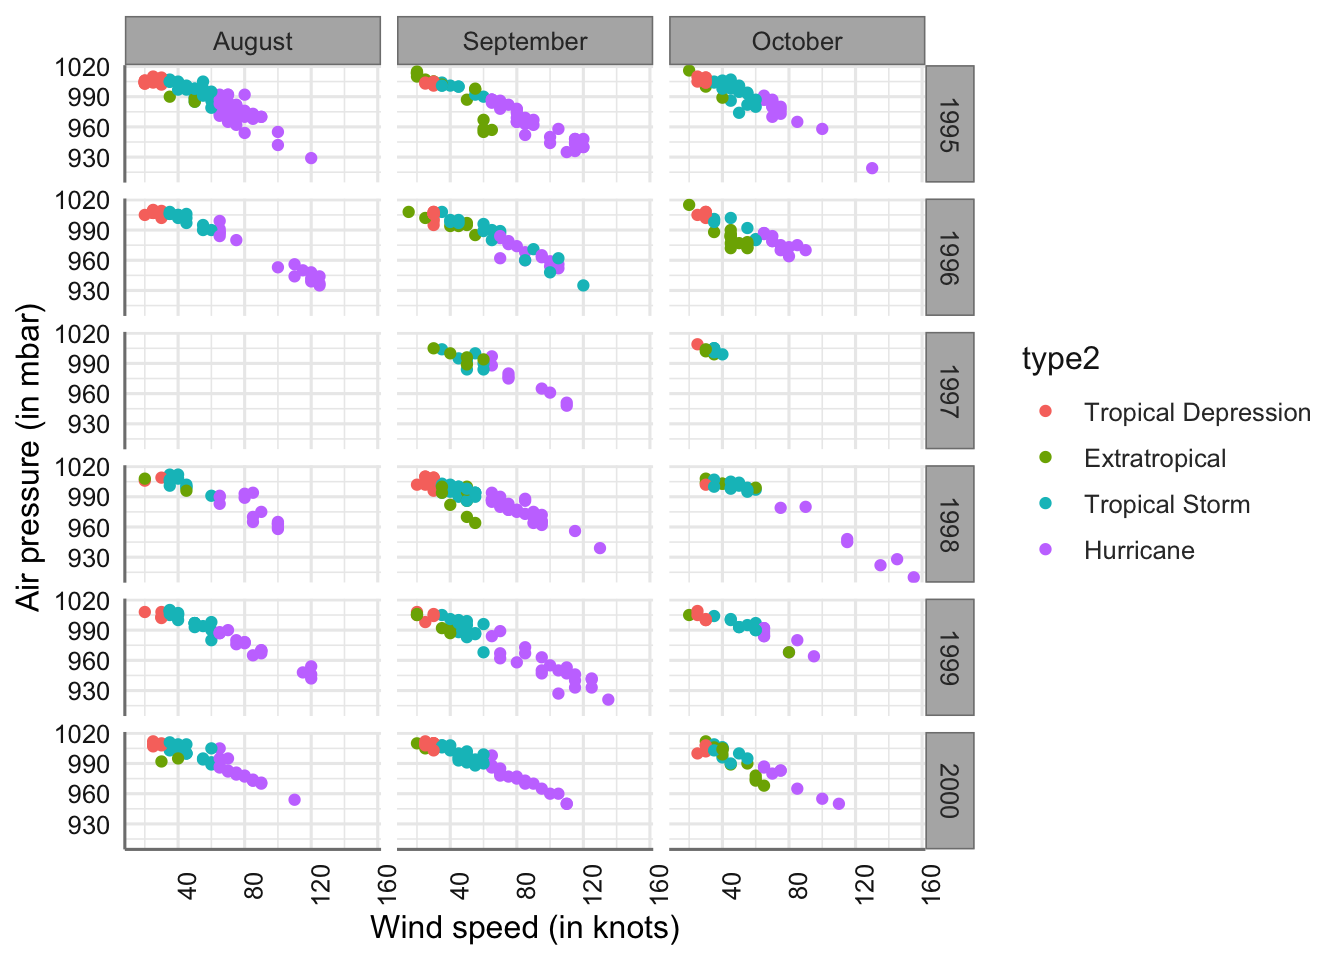
\includegraphics[width=0.95\linewidth]{02-aed_files/figure-latex/aed059-1} 

}

\caption{Gráfico de dispersion de presión vs velocidad para cada tipo de tormenta, año y mes.}\label{fig:aed059}
\end{figure}

¿Qué podemos decir de este gráfico?

\hypertarget{libreruxeda-de-interuxe9s}{%
\section{Librería de interés}\label{libreruxeda-de-interuxe9s}}

La libreria \texttt{ggplotgui} a través de la función \texttt{ggplot\_shiny} nos permite generar una aplicación con la que se puede obtener el código correspondiente a un gráfico. Para utilizar dicha función basta con escribir \texttt{ggplot\_shiny(dataframe)}.

\hypertarget{prob}{%
\chapter{Probabilidad}\label{prob}}

En esta unidad introducimos los conceptos básicos de varaible aleatoria, distribución de probabilidad, y las variables aleatorias más habituales en la investigación científica. No se trata de una unidad sobre probabilidad (para lo que se recomienda acudir a libros con mayores desarrollos), sino una unidad práctica de conocimiento básico de las distribuciones de probabilidad que juegan un papel relevante en los procesos de inferencia y en la cnstruccion de modelos estadísticos que veremos en las unidades siguientes.

\hypertarget{prob-intro}{%
\section{Introducción}\label{prob-intro}}

La probabilidad o el azar juega un papel muy importante en el razonamiento científico. Ejemplos de procesos biológicos donde la probabilidad juega un papel relevante son: i) la segregación de cromosomas en la formación de gametos o la ocurrencia de mutaciones genéticas. En otras ocasiones es el propio diseño experimental el que introduce la aleatoriedad como por ejemplo cuando dividimos un grupo de sujetos en función del tratamiento al que se van a ver sometidos.

Las conclusiones del análisis estadístico de datos se expresan en muchas ocasiones en términos de probabilidad, ya que implícitamente se está introduciendo la aleatoriedad debida a la muestra de sujetos con el que estamos trabajando, y que generalmente no coincide con toda la población bajo estudio.

En las unidades anteriores hemos visto que el estudio estadístico se centra en la información recogida sobre alguna variable relacionada directamente con el objetivo u objetivos del diseño experimental planteado. Un hecho cierto es que debido a la aleatoriedad e los sujetos resulta imposible saber con certeza el valor de dicha variable para un sujeto en particular. Se introduce de esta forma el concepto de \textbf{variable aleatoria} que hace referencia a todas aquellas en las que intrínsecamente se reconoce variabilidad en la respuesta de los sujetos.

En este punto introducimos algo de notación que nos resultará de utilidad de aquí en adelante. Las variables aleatorias siempre se denotan en mayúsculas, \(Y\), mientras que los valores observados para un conjunto de sujetos en esa variable (muestra) se denotan por minúsculas e indicando la posición que el sujeto ocupa en el banco de datos \(y_1,y_2,...,y_n\).

Por razones obvias se definen entonces las variables aleatorias discretas y las variables aleatorias continuas. Una variable discreta es aquella que sólo puede tomar un número finito o contable de posibles resultados, de forma que es posible conocer de antemano cuales son los posibles resultados que se pueden observar. Una variable continua es aquella que puede tomar infinitos valores numéricos, y por tanto es imposible identificar cada uno de los posibles valores de la variable, aunque si es posible conocer el rango de posibles resultados que se pueden observar. De forma natural se puede establecer una equivalencia entre la definición de variables categóricas y numéricas introducidas en unidades anteriores con las variables discretas y continuas.

Se puede describir de forma completa una variable aleatoria sin más que especificar la probabilidad asociada a cada uno de sus posibles valores. Esta especificación se conoce con el nombre de \textbf{distribución de probabilidad}. Sin embargo, la forma en que se puede especificar dicha distribución de probabilidad depende del tipo de variable aleatoria con la que estemos trabajando. En el caso de variables discretas basta con determinar la probabilidad de cada uno de los posibles resultados observables de la variable, pero no ocurre así en las variables continuas donde es imposible conocer todos sus posibles valores.

\hypertarget{distribuciones-modelos}{%
\section{Distribuciones-Modelos}\label{distribuciones-modelos}}

En la Unidad anterior se ha visto que el objetivo principal de muchos análisis estadísticos es estudiar el comportamiento de los sujetos de una población, a partir de la información recogida en una muestra de sujetos seleccionados de dicha población. Sin embargo, cuando hablamos de una población lo hacemos teniendo en mente las variables que se han medido sobre ellos. Imaginemos que estamos interesados en conocer la nota media de acceso de todos los estudiantes de primero de grado en la Universidad Miguel Hernández de Elche (UMH). En este caso es evidente que la población objetivo son todos los estudiantes de primero de grado que han accedido a la UMH, aunque esa población contiene información sobre muchas otras variables (sexo, edad, localidad de residencia,\ldots).Por lo tanto, todas las poblaciones se considerarán poblaciones de valores de alguna variable especificada. Si la población es infinita, nunca podremos obtener todos sus valores, e incluso si la población es finita, generalmente no queremos medir todos sus valores. En cualquier caso, deseamos obtener información sobre características particulares de la población a partir de un número restringido de valores de muestra. Por ejemplo, en el estudio de la nota de acceso podríamos querer utilizar la media de la nota media de todos los estudiantes como referencia de la población, aunque podríamos utilizar otros como el percentil 80, etc\ldots{}

Para proceder de esta forma, necesitamos formular un modelo adecuado para los valores \(x\) que componen la población, relacionar las características de interés con los aspectos apropiados del modelo y luego usar los datos de la muestra para proporcionar estimaciones de estos aspectos.La característica esencial de tales valores \(x\) en su imprevisibilidad, y lo mejor que podemos hacer es especificar la probabilidad de obtener un valor dado o un valor en un rango dado. Por lo tanto, las distribuciones de probabilidad proporcionan los modelos más apropiados para las poblaciones variables de respuesta. Más específicamente, la función de densidad de probabilidad \(f(x)\) o la función de distribución de probabilidad \(F(x)\) proporcionan la información necesaria, por lo que constituye el modelo de población para la variable aleatoria \(X\). Por supuesto, dado que nunca conocemos esta distribución con una certeza total, debemos suponer una forma funcional específica (modelo matemático) para \(f(x)\) y \(F(x)\). Esta forma funcional usualmente involucra uno o más parámetros que pueden ser variados, y leso que se espera es que habrá algunos valores específicos de estos parámetros para los cuales la distribución resultante se ajusta adecuadamente a nuestros datos observados. Tal modelo se llama \textbf{modelo paramétrico} para \(X\). En el tema siguiente se presentarán los modelos paramétricos más frecuentes para una variable aleatoria \(X\).

Por el momento, supongamos que hemos especificado alguna función adecuada \(f(x)\) como la densidad de probabilidad de nuestra población. ¿Qué valores resumen de esta densidad se relacionan con las características de la población que generalmente son de interés? Para responder a esta situación, centrémonos en las variables discretas e interpretemos la probabilidad como una frecuencia relativa. Si la variable aleatoria \(X\) tiene valores posibles \(x_1, x_2, x_3, ... ,x_n\) y si \(p_i = P(X = x_i)\), entonces podemos pensar en \(p_i\) como la frecuencia relativa con la que el valor \(x_i\) ocurre en toda la población.

Definimos el valor esperado de \(X\) por la ecuación:

\begin{equation} 
  E(X) = \sum_{i=1}^n  x_i p_i
  \label{eq:espdisc}
\end{equation}

Utilizando la interpretación de frecuencia relativa de \(p_i\) dada anteriormente, \(E(X)\) puede interpretarse como el promedio de los valores \(X\) en toda la población, por lo que es la media poblacional. Este es claramente uno de los principales valores de resumen para la población. A menudo se denota \(\mu\) y como mide el ``centro'' de la población también se lo conoce como el parámetro de localización de la población.

De forma similar se define la varianza de la población, \(\sigma2\), como:

\begin{equation} 
  \sigma^2 = V(X) = E\{(X-\mu)^2\} = \sum_{i=1}^n  (x_i - \mu)^2 p_i
  \label{eq:vardisc}
\end{equation}

La desviación típica poblacional, \(\sigma\), se obtiene a partir de la raíz cuadrada de la varianza poblacional:

\begin{equation} 
  \sigma = DT(X) = \sqrt{V(X)}
  \label{eq:sddisc}
\end{equation}

Siguiendo con el ejemplo de la variable aleatoria que representa la suma del lanzamiento de dos dados ¿Cuál es el valor esperado de la suma de ambos lanzamientos? ¿Cuál es la desviación típica? En este caso ¿la distribución es aproximada o la distribución poblacional?

En el caso de variables aleatorias continuas, donde denotamos por \(R\) el rango de todos los valores posibles, se define la media, varianza y desviación típica poblacional como

\begin{equation} 
  \mu = E(X) = \int_R x f(x) dx
  \label{eq:espcont}
\end{equation}

\begin{equation} 
  \sigma^2 = V(X) = \int_R (x - \mu)^2 f(x) dx
  \label{eq:varcont}
\end{equation}

\begin{equation} 
  \sigma = DT(X) = \sqrt{V(X)}
  \label{eq:sdcont}
\end{equation}

Para las variables de tipo continuo más habituales la esperanza, varianza y desviación típica poblacionales se aproximan de forma precisa (si la muestra de trabajo es adecuada) por la media, varianza y desviación típica muestral.

\hypertarget{distribuciones-notables}{%
\section{Distribuciones notables}\label{distribuciones-notables}}

En la práctica resultaría complicado y farragoso si para cada experimento aleatorio ligeramente diferente de otro ya realizado, tuviéramos que determinar las distribuciones de probabilidad desde cero. Afortunadamente, podemos hacer uso de las similitudes que existen entre ciertos tipos o familias de experimentos y ciertas distribuciones de probabilidad, conocidas con el nombre de \textbf{distribuciones notables}, que nos permiten el desarrollo de las funciones de distribución que representen las características generales del experimento.

Por ejemplo, muchos experimentos comparten el elemento común de que sus resultados se pueden clasificar en uno de dos eventos: una moneda puede salir cara o cruz; un niño puede ser hombre o mujer; una persona puede morir o no morir; una persona puede ser empleada o desempleada. Estos resultados a menudo se etiquetan como ``éxito'' o ``fracaso'', teniendo en cuenta que aquí no hay connotación de ``bondad''; por ejemplo, al observar los nacimientos, el estadístico podría calificar el nacimiento de un niño como un ``éxito'' y la el nacimiento de una niña como un ``fracaso'', pero los padres no necesariamente verían las cosas de esa manera. Esta situación experimental se conoce como experimento Bernouilli, asignando probabilidad \(\theta\) al suceso calificado como éxito y probabilidad \(1-\theta\) al suceso calificado como de fracaso. Dichas probabilidades son diferentes para cada situación y se pueden aproximar mediante la obtención de datos experimentales. La distribución de probabilidad que surge en este experimento se conoce como distribución Bernouilli y es la primera distribución de probabilidad notable conocida.

\hypertarget{prob-binomial}{%
\subsection{Distribución Binomial}\label{prob-binomial}}

A menudo nos interesa el resultado de los ensayos independientes y repetidos de Bernoulli, es decir, el número de éxitos en ensayos repetidos. En esta situación se considera:

\begin{enumerate}
\def\labelenumi{\arabic{enumi}.}
\tightlist
\item
  sucesos independientes: el resultado de un ensayo no afecta el resultado de otro ensayo.
\item
  repeticiones: las condiciones son las mismas para cada prueba, es decir, la probabilidad de éxito y fracaso permanecen constantes a través de los diferentes ensayos realizados.
\end{enumerate}

Una distribución binomial nos da las probabilidades asociadas con los ensayos independientes y repetidos de Bernoulli. En una distribución binomial, las probabilidades de interés son las de observar un cierto número de éxitos, \(r\), en \(n\) ensayos independientes, cada uno de los cuales tiene solo dos resultados posibles y la misma probabilidad, \(\theta\), de éxito. Por ejemplo, usando una distribución binomial, podemos determinar la probabilidad de obtener 4 caras en 10 lanzamientos de una misma moneda.

La distribución de probabilidad para este experimento queda completamente determinado si conocemos \(n\) (número de repeticiones realizadas) y \(\theta\) (probabilidad de éxito). Si \(X\) denota la variable aleatoria asociada con este experimento, la función de densidad de probabilidad se define como:

\begin{equation} 
  P(X = x) = {n \choose x} \theta^x (1-\theta)^{n-x}
  \label{eq:probbinom}
\end{equation}

donde \({n \choose x}\) representa el número combinatorio de \(n\) sobre \(x\), y \(x\) el número de éxitos observados. Dicha distribución se denota habitualmente:

\begin{equation} 
  X \sim Bi(n, \theta)
  \label{eq:varbinom}
\end{equation}

Esta distribución se puede evaluar para cualquier valor entre 0 y el número de repeticiones del experimento \(n\). En \texttt{R} la función \texttt{dbinom} permite obtener cualquier probabilidad de la distribución binomial una vez fijamos el valor que deseamos evaluar (\(x\)), el número de repeticiones (\(n\)), y la probabilidad de éxito asociada (\(\theta\)).

Una vez establecida la función de densidad de probabilidad resulta posible obtener el valor esperado del número de éxitos, así como conocer su variabilidad haciendo uso de las definiciones expuestas en el tema anterior. En concreto, para una variable que sigue una distribución de probabilidad Binomial (\eqref{eq:varbinom}) tenemos que:

\begin{equation} 
  E(X) = n \theta
  \label{eq:espbinom}
\end{equation}

\begin{equation} 
  V(X) = n \theta (1-\theta)
  \label{eq:varbinom}
\end{equation}

\begin{equation} 
  DT(X) = \sqrt{n \theta (1-\theta)}
  \label{eq:sdbinom}
\end{equation}

En la página web \url{http://www.artofstat.com/} se encuentra disponible una aplicación de trabajo de la distribución Binomial (\url{https://istats.shinyapps.io/BinomialDist/}). Dicha aplicación nos permite calcular tanto probabilidades como cuantiles para un experimento binomial. Utiliza dicha aplicación para responder a las cuestiones siguientes:

\begin{itemize}
\tightlist
\item
  En una población de sujetos se conoce que el 39\% de ellos sufre algún tipo de mutación genética. Si se obtiene una muestra de 20 sujetos ¿cuál es la probabilidad de observar tres sujetos con esa mutación genética?
\item
  En una población de moscas de la fruta se conoce que el 30\% son de color negro y el 70\% son de color gris. Si se extrae una muestra de 15 moscas ¿cuál es la probabilidad de observar al menos cuatro moscas de color negro? ¿y de color gris?
\item
  Una cierta droga causa daños en el hígado en el 1\% de los pacientes. Se van a realizar estudios completos sobre 50 pacientes que están tomando dicha droga para detectar daños en el hígado. ¿Cuál es la probabilidad de que ninguno de lo pacientes muestre daños en el hígado? ¿Cuál es la probabilidad de que al menos uno de los pacientes muestre daños en el hígado?
\item
  Los estudios realizados concluyen que el 10\% de las adolescentes de EEUU tienen deficiencia de hierro. Se obtiene una muestra de 14 adolescentes y se desea conocer ¿cuál es la probabilidad de que al menos el 50\% de ellas tengan una deficiencia de hierro?
\item
  En un experimento se comprobó que la aplicación de un tratamiento químico aumentaba la resistencia a la corrosión de un material en un 80 \% de los casos. Si se tratan ocho piezas, determina: (i) probabilidad de que el tratamiento sea efectivo para más de cinco piezas, (ii) probabilidad de que el tratamiento sea efectivo para al menos tres piezas, (iii) número de piezas para las que espera que el tratamiento sea efectivo.
\item
  Se dispone de un cristal que tiene dos tipos de impurezas que absorben radiación de la misma longitud de onda. Una de ellas emite un electrón tras la absorción de un fotón, mientras que la segunda no emite electrones. Las impurezas están en igual concentración y distribuidas homogéneamente en el cristal. Sin embargo, la sección eficaz de absorción, que es una medida de la probabilidad de absorber un fotón, es 90 veces mayor para la impureza que emite electrones que el de la impureza que no los emite. Suponiendo que sobre el cristal inciden 200 fotones y que este es lo suficientemente grande para absorber todos, calcula la probabilidad de que al menos se emitan tres electrones.
\end{itemize}

\hypertarget{prob-poisson}{%
\subsection{Distribución Poisson}\label{prob-poisson}}

La distribución de Poisson se emplea como un modelo para variables aleatorias de tipo discreto cuando se quieren obtener las probabilidades de ocurrencia de un evento que se distribuye al azar en el espacio o el tiempo. Algunos ejemplos de esta distribución son:

\begin{itemize}
\tightlist
\item
  En el estudio de cierto organismo acuático, se toman un gran número de muestras de un lago y se cuentan el número de organismos que aparecen en cada muestra. El interés principal radica en conocer cuál es la probabilidad de encontrar algún organismo en una muestra próxima si la media observada en el conjunto de nuestras es de 2 organismos.
\item
  En un estudio sobre la efectividad de un insecticida sobre cierto tipo de insecto, se fumiga una gran región. Posteriormente se crea una cuadrícula sobre el terreno, se selecciona de forma aleatoria un conjunto de ellas, y se cuenta el número de insectos vivos dentro de cada una. Estamos interesados en conocer cuál es la probabilidad de que no encontremos ningún insecto vivo en una cuadrícula próxima si se sabe que que la media de insectos vivos en las cuadriculas analizadas es de 0.5.\\
\item
  Un grupo de investigadores observó la ocurrencia de hemangioma capilar retiniano (RCH) en pacientes con la enfermedad de von Hippel-Lindau (VHL). RCH es un tumor vascular benigno de la retina. Usando una revisión retrospectiva de series de casos consecutivos, los investigadores encontraron que el número de medio de tumores RCH por ojo para pacientes con VHL era de 4. Están interesados en conocer cuál es la probabilidad de que se detecten más de cuatro tumores por ojo.
\end{itemize}

Como se puede ver en los ejemplos la distribución de Poisson es muy habitual en los campos de la biología y la medicina. En una distribución de Poisson, las probabilidades de interés son las de observar un número de eventos, \(x\), en un tiempo o espacio determinado. La distribución de probabilidad para este experimento queda completamente determinada si conocemos el número de eventos y \(\lambda\) la tasa o media del número de eventos que ocurren por unidad de tiempo o espacio. Si \(X\) denota la variable aleatoria asociada con este experimento, la función de densidad de probabilidad se define como:

\begin{equation} 
  P(X = x) = \frac{e^{-\lambda} \lambda^x}{x!}
  \label{eq:probpois}
\end{equation}

Dicha distribución se denota habitualmente: \[ X \sim Po(\lambda)\]. Esta distribución se puede evaluar para cualquier valor entre 0 y el número de máximo de ocurrencias que pueden ocurrir. Dado que este valor no se conoce de antemano se debe prefijar un valor máximo que asegure que la probabilidad de ese valor sea cero.

En \texttt{R} la función \texttt{dpois} permite obtener cualquier probabilidad de la distribución de Poisson una vez fijamos el valor que deseamos evaluar (\(x\)), y la tasa o media del número de eventos (\(\lambda\)).

Una vez establecida la función de densidad de probabilidad resulta posible obtener el valor esperado del número de eventos ocurridos, así como conocer su variabilidad haciendo uso de las definiciones expuestas en el tema anterior. En concreto, para una variable que sigue una distribución de probabilidad Poisson (\(X \sim Po(\lambda)\)) tenemos que:

\begin{equation} 
  E(X) = \lambda
  \label{eq:meanpois}
\end{equation}

\begin{equation} 
  V(X) = \lambda
  \label{eq:varpois}
\end{equation}

\begin{equation} 
  DT(X) = \sqrt{\lambda}
  \label{eq:sdpois}
\end{equation}

En la página web \url{http://www.artofstat.com/} se encuentra disponible una aplicación de trabajo de la distribución Binomial (\url{https://istats.shinyapps.io/PoissonDist/}). Dicha aplicación nos permite calcular tanto probabilidades como cuantiles para un experimento poisson Utiliza dicha aplicación para responder a las cuestiones siguientes:

(Hint: Recuerda que la tasa de la poisson se debe modificar si las cuestiones de interés no están referenciadas a la misma escala que la escala proporcionada).

\begin{itemize}
\tightlist
\item
  Un laboratorio es capaz de realizar 20 análisis de cierto tipo en un hora. ¿Cuál es la probabilidad de realizar entre 30 y 36 análisis en las próximas dos horas?¿y la probabilidad de realizar más de 36? (Hint: En este caso no concemos directamente la media de la poisson ya que la escala medida no es la misma sobre la que se este interesado, por lo que es necesario ajustar la tasa a cada pregunta)
\item
  Consideremos que el número de trozos de chocolate en una determinada galleta sigue una distribución de Poisson. Queremos que la probabilidad de que una galleta seleccionada al azar tenga por lo menos tres trozos de chocolate sea mayor que 0.8. Encontrar el valor entero más pequeño de la media de la distribución que asegura esta probabilidad.
\item
  Un fabricante de maquinaria pesada tiene instalados en el campo 3840 generadores de gran tamaño con garantía. Sí la probabilidad de que cualquiera de ellos falle durante el año dado es de 1/1200 determine la probabilidad de que a) 4 generadores fallen durante el año en cuestión, b) que más 1 de un generador falle durante el año en cuestión.
\item
  En un proceso de manufactura, en el cual se producen piezas de vidrio, ocurren defectos o burbujas, ocasionando que la pieza sea indeseable para la venta. Se sabe que en promedio 1 de cada 1000 piezas tiene una o más burbujas. ¿Cuál es la probabilidad de que en una muestra aleatoria de 8000 piezas, menos de 3 de ellas tengan burbujas?
\item
  Se sabe que el número de microorganismos por gramo de una cierta muestra de suelo diluida en agua destilada se distribuye según una variable aleatoria de media 0.08. Si una preparación con un gramo de esta disolución se vuelve turbia, este gramo contiene al menos un microorganismo. Hallar la probabilidad de que una preparación que se ha vuelto turbia contenga:

  \begin{itemize}
  \tightlist
  \item
    Un solo microorganismo
  \item
    Menos de tres microorganismos
  \item
    Más de dos microorganismos
  \end{itemize}
\item
  En un monte, el número de plantas de romero por círculo de un metro de radio, se distribuye según una variable aleatoria. Se eligen 1o plantas al azar y se mide la distancia a la planta que tiene más próxima. Las distancias observadas fueron (medidas en metros): 0.7, 1.7, 1.2, 0.4, 0.2, 0.5, 0.7, 0.8, 1.5, y 2.1. A partir de estos datos estima los parámetros de interés de la distribución y calcula cuantas plantas es de esperar que habrá en una zona del monte de unos 12500 m2 de superficie.
\end{itemize}

\hypertarget{prob-normal}{%
\subsection{Distribución Normal}\label{prob-normal}}

Hasta ahora todas las distribuciones consideradas eran de tipo de discreto. En este punto tratamos la distribución de probabilidad de tipo continuo y más concreta mente la más famosa y utilizada de todas ellas: la distribución de probabilidad Normal. Una variable de tipo continuo es aquella que puede tomar cualquier valor dentro de un rango de valores, es decir, existe un infinito número de valores posibles para la variable aleatoria. Para representar gráficamente una distribución de una variable aleatoria continua se debe construir un subconjunto de clases o intervalos consecutivos para el rango de valores de la variable considerada y considerar el histograma resultante. Cuando consideramos un número muy grande de clases o intervalos podríamos obtener la curva suavizada que representa la función de densidad de probabilidad de la variable aleatoria.

La función de densidad de probabilidad para una variable aleatoria \(X\) que sigue una distribución Normal con parámetros \(\mu\) y \(\sigma\), denotada por \(N(\mu, \sigma^2)\) viene dada por:
\begin{equation} 
  f(x) = \frac{1}{2\pi\sigma^2} exp\left(-\frac{(x - \mu)^2}{2\sigma^2}\right)
  \label{eq:densinormal}
\end{equation}

Los dos parámetros de la distribución son \(\mu\) que representa la medida de localización y \(\sigma\) la medida de dispersión. Habitualmente los conocemos por sus nombres más habituales como son la media y la desviación típica. En concreto, para una variable que sigue una distribución de probabilidad Normal (\(X \sim N(\mu, \sigma^2)\)) tenemos que:

\begin{equation} 
  E(X) = \mu
  \label{eq:meannormal}
\end{equation}

\begin{equation} 
  V(X) = \sigma^2
  \label{eq:varnormal}
\end{equation}

\begin{equation} 
  DT(X) = \sigma
  \label{eq:sdnormal}
\end{equation}

Las características más importantes de la distribución Normal:

\begin{itemize}
\tightlist
\item
  Es una distribución simétrica alrededor de la media, \(\mu\).
\item
  La media, la mediana y la moda son iguales.
\item
  La distribución Normal queda completamente especificada a partir de los valores de \(\mu\) y \(\sigma\). Los diferentes valores de la media y la desviación típica desplazan hacia un lado o el otro, o consiguen una distribución más puntiaguda (desviaciones típicas más pequeñas) o más achatada (desviaciones típicas más grandes).
\item
  El intervalo definido por \(\mu - 5 * \sigma, \mu + 5 * \sigma\) tiene probabilidad 1, es decir, la probabilidad de los extremos inferior y superior del rango de valores se puede considerar despreciable.\\
\item
  Dada una variable aleatoria Normal con media \(\mu\) y desviación típica \(\sigma\) y tenemos un escalar \(a\) tenemos que:
\end{itemize}

\[ X \sim N(\mu, \sigma^2) \Longrightarrow aX \sim N(a\mu, a^2\sigma^2)\]
* Dada dos variables aleatorias Normales, \(X e Y\), con medias y desviaciones típicas respectivas: \(\mu_1\), \(\sigma_1\) y \(\mu_2\), \(\sigma_2\) y dos escalares \(a\) y \(b\) tenemos que

\[ X \sim N(\mu_1, \sigma^2_1), Y \sim N(\mu_2, \sigma^2_2) \Longrightarrow aX + bY\sim N(a\mu_1+b\mu_2, a^2\sigma^2_1+b^2\sigma^2_2)\]

Esta última propiedad se puede generalizar para el caso de \(m\) variables aleatorias en lugar de 2.

\hypertarget{teorema-central-de-luxedmite}{%
\subsubsection{Teorema Central de Límite}\label{teorema-central-de-luxedmite}}

Si las variables aleatorias \(X_1,...X_n\) son una muestra aleatoria de una distribución con media \(\mu\) y desviación típica \(\sigma\) entonces las variables aleatorias suma (\(T = X_1+...+X_n\)) y media (\(M = (X_1+...+X_n)/n\)) tienen distribuciones:
\[ T \sim N\left(n\mu,n\sigma^2\right)\]
\[ M \sim N\left(\mu,\frac{\sigma^2}{n}\right)\]

En la página web \url{http://www.artofstat.com/} se encuentra disponible una aplicación de trabajo de la distribución Binomial (\url{https://istats.shinyapps.io/NormalDist/}). Dicha aplicación nos permite calcular tanto probabilidades como cuantiles para un experimento normal Utiliza dicha aplicación para responder a las cuestiones siguientes:

\begin{itemize}
\tightlist
\item
  La longitud L (en micras) de ciertas larvas parásitas de moluscos, sigue la distribución Normal, pero de media y desviación típica distinats, según la larva se encuentre en estadio 1 o en estadio 2 de su crecimiento. La media y la desviación típica son: 219 y 20 para el estadio 1, y 241 y 14 para el estadio 2. Para identificar el estadio en que se encuentra la larva, se adopta el criterio siguiente: Si L≤230 pertenece al estadio 1, en otro caso pertenece al estadio 2. Resolver las siguientes cuestiones:

  \begin{itemize}
  \tightlist
  \item
    Calcular la probabilidad de la presencia del suceso L≤230 para larvas del estadio 1. Idem. para larvas en el esatdio 2.
  \item
    Desde que nace una larva hasta que llega al estadio 3 de su desarrollo (que es fácilmente identificable), trasncurren 12 horas, permaneciendo 8 horas en el estadio 1 y 4 horas en el estadio 2. La observación de una larva cualquiera se hace en un instante que puede considerarse elegido al azar durante estas 12 horas (se desconoce cuando ha nacido la larva). Entonces, si se ha observado que una larva mide L = 225 y, por lo tanto, se considera que pertenece al estadio 1, calcular la probabilidad de equivocarnos al tomar esta decisión.
  \end{itemize}
\item
  Supongamos que el diámetro de las aceitunas rellenas de anchoa varía entre 15 y 17 mm. Debido a al sequía del último año, la producción de aceituna verde se ha distribuido según una normal de media 15.5 mm. y desviación típica 1.2 mm. ¿Qué porcentaje de aceitunas podría ser aprovechado para rellenar de anchoa?
\item
  La duración media de un lavavajillas es de 15 años y su desviación típica 0.5. Sabiendo que la vida útil del lavavajillas se distribuye normalmente, hallar la probabilidad de que al adquirir un lavavajillas, este dure más de 15 años.
\item
  Una normativa europea obliga a que en los envases de yogur no debe haber menos de 120 gr. La máquina dosificadora de una empresa láctea hace los envases de yogur según una distribución normal de desviación típica de 2 gr. y media 122 gr.

  \begin{itemize}
  \tightlist
  \item
    ¿Qué tanto por ciento de los envases de yogur de esa empresa cumplirá la normativa?
  \item
    ¿Cuál deberá ser la media de la distribución normal con la cual la máquina dosificadora debe hacer los envases para que el 98\% de la producción de yogures de la empresa cumpla la normativa?. (La desviación típica sigue siendo de 2 gr.).
  \end{itemize}
\end{itemize}

\hypertarget{otras-distribuciones}{%
\subsection{Otras distribuciones}\label{otras-distribuciones}}

A partir de la distribución de probabilidad Normal se pueden obtener otras distribuciones de probabilidad que resultan de gran utilidad para los procesos de generalización de resultados de un diseño experimental a una población que veremos en la unidad siguiente.

\hypertarget{distribuciuxf3n-chi-cuadrado}{%
\subsubsection{Distribución Chi-cuadrado}\label{distribuciuxf3n-chi-cuadrado}}

Sean n variables aleatorias \(X_1,...,X_n\) independientes entre sí cuya distribución de probabilidad es idéntica para todas ellas e igual a una Normal estándar (\(N(0,1)\)). Si definimos la variable aleatoria suma como:
\[X = X_1 + ... + X_n,\] entonces decimos que \(X\) se distribuye según una distribución Chi-cuadrado con \(n\) grados de libertad y la denotamos por \[X \sim \chi^2_n.\]

\hypertarget{t-se-student}{%
\subsubsection{T se Student}\label{t-se-student}}

Si tenemos dos variables aleatorias independientes \(Y\) y \(Z\) con distribuciones de probabilidad
\[Z \sim N(0,1); Y \sim \chi^2_n,\] y consideramos la variable aleatoria \(X\) dada por:
\[X = \frac{Z}{\sqrt{Y/n}},\] entonces decimos que dicha variable sigue una distribución \(t\) de Student con \(n\) grados de libertad, y se denota por
\[X \sim t_n.\]

\hypertarget{f-de-snedecor}{%
\subsubsection{F de Snedecor}\label{f-de-snedecor}}

Si tenemos dos variables aleatorias independientes \(Y\) y \(Z\) con distribuciones de probabilidad
\[Z \sim \chi^2_n; Y \sim \chi^2_m,\] y consideramos la variable aleatoria \(X\) dada por:
\[X = \frac{Z/n}{Y/m},\] entonces decimos que dicha variable sigue una distribución \(F\) de Snedecor con \(n\) y \(m\) grados de libertad, y se denota por
\[X \sim F_{n,m}.\]

\hypertarget{inferencebasica}{%
\chapter{Inferencia básica}\label{inferencebasica}}

En la unidad anterior se han expuesto brevemente la teoría y los métodos de la probabilidad. En este unidad se expondrán la teoría y los métodos de la inferencia estadística que servirán como base para los modelos estadísticos que estudiaremos en la unidad siguiente. Un problema de inferencia estadística es un problema en el cual se han de analizar datos que han sido generados de acuerdo con una distribución de probabilidad desconocida y en la que se debe realizar algún tipo de inferencia (``conocer su comportamiento'') acerca de tal distribución. En la mayoría de situaciones reales, existe un número infinito de distribuciones posibles distintas que podrían haber generado los datos. En la práctica, dado el tipo de variable aleatoria considerada, se suele asumir un modelo de distribución de probabilidad que es completamente conocida salvo excepto por los valores de los parámetros que la especifican completamente. Utilizamos los datos de la muestra para obtener información sobre dichos parámetros desconocidos y poder asumir de esta forma una distribución de probabilidad completa para todos los datos de la población.

Por ejemplo, se podría saber que la duración de cierto tipo de marcapasos tiene una distribución exponencial con parámetro \(\lambda\) pero desconocer el valor exacto de dicho parámetro. Si se puede observar la duración de varios marcapasos de este tipo, entonces, a partir de estos valores observados y de cualquier otra información relevante de la que se pudiera disponer, es posible producir una inferencia acerca de ese valor desconocido \(\lambda\). Podría interesar producir la mejor estimación del valor de dicho parámetro o especificar un intervalo en el cual se piensa que pueda estar incluido el verdadero valor de \(\lambda\), o decidir si dicho parámetro es menor que un valor específico, ya que en ningún caso es posible obtener el verdadero valor de \(\lambda\) ya que sería necesario obtener la información de todos los sujetos de la población y no sólo los de la muestra.

En un problema de inferencia estadística, cualquier característica de la distribución que genera los datos experimentales que tenga un valor desconocido, como \(\lambda\) en el ejemplo anterior, se llama parámetro de la distribución. El conjunto \(\Omega\) de todos los valores posibles de dicho parámetro se llama espacio parámetrico. Cuando nuestra distribución de probabilidad tiene dos parámetros (por ejemplo la distribución Normal) el espacio paramétrico vendrá dado por todo el conjunto de parejas de valores de \(\mu\) y \(\sigma^2\).

\hypertarget{estimador-y-estimaciuxf3n}{%
\section{Estimador y estimación}\label{estimador-y-estimaciuxf3n}}

Si tenemos una variable aleatoria \(X\) cuya función de distribución viene caracterizada por un parámetro o conjunto de parámetros \(\delta\), y una muestra aleatoria de tamaño \(n\), \(X_1,...,X_n\), a partir de la cual se observan el conjunto de datos muestrales \(x_1,...,x_n\) vamos a definir dos conceptos relevantes en todo proceso de inferencia: \texttt{estimador} y \texttt{estimación}.

Un \textbf{estimador} del parámetro \(\delta\), basado en las variables aleatorias \(X_1,...,X_n\), es una función \(\delta(X_1,...,X_n)\) que especifica una valor para \(\delta\). Se trata de una función matemática que tiene la misma forma independientemente de la muestra utilizada. Por ejemplo, los estimadores para la media, varianza (y cuasivarainza), y proporción poblacionales vienen dados por:

\begin{enumerate}
\def\labelenumi{\arabic{enumi}.}
\tightlist
\item
  Media muestral
\end{enumerate}

\[\delta_1(X_1,...,X_n) = \bar{X} = \frac{X_1+X_2+...+X_n}{n}\]

\begin{enumerate}
\def\labelenumi{\arabic{enumi}.}
\setcounter{enumi}{1}
\tightlist
\item
  Varianza muestral
\end{enumerate}

\[\delta_2(X_1,...,X_n) = S^2 = \frac{\sum_{i=1}^n (X_i-\bar{X})^2}{n}\]

\begin{enumerate}
\def\labelenumi{\arabic{enumi}.}
\setcounter{enumi}{2}
\tightlist
\item
  Cuasi-Varianza muestral
\end{enumerate}

\[\delta_3(X_1,...,X_n) = S_q^2 = \frac{n}{n-1} S^2\]

Para una variable de tipo discreto se aplican las mismas definiciones si consideramos cada \(X_i\) como una realización de dicha variable. Para una variable que mide ``éxito'' o ``fracaso'' los valores de \(X_i\) serán 1 o 0 respectivamente, de forma que la media muestral coincide con la proporción muestral ya que tendríamos la suma de 1 en el numerador dividido por el tamaño de muestra en el denominador.

Una \textbf{estimación} es el valor numérico del estimador para unos datos dados (\(x_1,...,x_n\)), es decir, sustituimos en \(\delta(X_1,...,X_n)\) por sus valores observados y obtendríamos la estimación del parámetro. De forma habitual se identifica con el ``gorro'' encima del parámetro indica la estimación de un parámetro: \[\hat{\mu} = \delta_1(x_1,...,x_n) =\bar{x}\] \[\hat{\sigma}^2 = \delta_2(x_1,...,x_n)= s^2\]

\hypertarget{informaciuxf3n-contenida-en-la-muestra}{%
\section{Información contenida en la muestra}\label{informaciuxf3n-contenida-en-la-muestra}}

Antes de comenzar a describir los procesos de inferencia estadística es necesario conocer como podemos relacionar la información contenida en una muestra con la distribución de probabilidad de la variable aleatoria de interés. Para ello una vez fijada la población del estudio y el objetivo principal es necesario:

\begin{itemize}
\tightlist
\item
  Establecer la variable de interés, \(X\) (y su tipo), en función del objetivo principal
\item
  Establecer una distribución de probabilidad para la variable aleatoria, \(f(X | \theta)\), acorde con el tipo de dicha variable y lo más sencilla posible, donde \(\theta\) representa el parámetro o parámetros que especifican dicha distribución.
\item
  Muestra aleatoria de tamaño \(n\) de la variable de interés, \(X_1, X_2,...,X_n\) de forma que cada observación tiene probabilidad \(f(X_1 | \theta), f(X_2 | \theta),...,f(X_n | \theta)\) respectivamente y sus valores observados vienen dados por \(x_1,...,x_n\).
\item
  Obtener los descriptivos muestrales habituales: media, varianza, desviación típica, o proporción.
\end{itemize}

Se define entonces la \texttt{función\ de\ verosimilitud} \(L(X|\theta)\) como: \[L(X|\theta) = \prod_{i=1}^n f(X_i|\theta) = f(X_1|\theta)f(X_2|\theta)\cdots f(X_n|\theta)\]

La función de verosimilitud contiene toda la información sobre la muestra y la relaciona con el parámetro o parámetros de interés a través de la distribución de probabilidad establecida. Se convierte por tanto en la herramienta más importante, desde el punto de vista de la estadística frecuentista, para los procesos de inferencia estadística que estudiaremos a continuación. Además, se utiliza como base para la caracterización de la distribución en el muestreo de los diferentes estimadores, aproximaciones numéricas del verdadero valor del parámetro o parámetros de la distribución de probabilidad asumida, que se utilizan en los procesos inferenciales.

Para evitar la complejidad matemática que supone trabajar con productos se suele definir el logaritmo de la función de verosimilitud, \texttt{log-verosimilitud}, \(LL(X|\theta)\) como: \[LL(X|\theta) = log\left(\prod_{i=1}^n f(X_i|\theta)\right) = \sum_{i=1}^n log(f(X_i|\theta)) = log(f(X_1|\theta))+log(f(X_2|\theta))+\cdots +log(f(X_n|\theta))\]

\hypertarget{procedimientos-de-inferencia-estaduxedstica}{%
\section{Procedimientos de inferencia estadística}\label{procedimientos-de-inferencia-estaduxedstica}}

Estudiamos en este punto los distintos procedimientos de inferencia que tratamos en esta unidad. Realizamos una pequeña introducción de cada uno de ellos y ejemplificaremos su uso en el análisis de una población.

\hypertarget{estimaciuxf3n-puntual}{%
\subsection{Estimación puntual}\label{estimaciuxf3n-puntual}}

Es el procedimiento de inferencia estadística más sencillo y consiste en obtener un único valor aproximado del parámetro de interés a partir de un estimador de dicho parámetro y de los datos observados de una muestra. Aunque en las situaciones más sencillas (media, varianza y proporción) tanto el estimador como la estimación son fáciles de obtener, hay que establecer un procedimiento general para obtener dichas estimaciones.

Dicho procedimiento consiste en encontrar el máximo de la función de verosimilitud (o más concretamente de la log-verosimilitud) para el parámetro o parámetros involucrados en dicha función, es decir, el valor o valores que se obtienen al igualar a cero la derivada de la función de log-verosimilitud: \[\frac{d}{d\theta} LL(X | \theta) = 0\]

\hypertarget{estimador-de-una-proporciuxf3n}{%
\subsubsection{Estimador de una proporción}\label{estimador-de-una-proporciuxf3n}}

La estimación de proporciones surge de forma natural en poblaciones Bernouilli cuya función de log-verosimilitud viene dada por: \[LL(X |\theta) = s*log(\theta) + (n-s)*log(1-\theta)\] Derivando e igualando a cero: \[\frac{d}{d\theta} LL(X | \theta) = \frac{s}{\theta}+\frac{-(n-s)}{1-\theta} = 0\] Despejando obtenemos: \[\hat{\theta} = \frac{s}{n}\] que es el estimador habitual para obtener la proporción muestral.

\hypertarget{estimador-de-una-media}{%
\subsubsection{Estimador de una media}\label{estimador-de-una-media}}

Si asumimos que la variable aleatoria es \(N(\mu,\sigma^2)\) la función de log verosimilitud viene dada por:

\[LL(X |\mu,\sigma^2) = -\frac{n}{2}*log(2\pi\sigma^2)+\frac{nS^2 + n(\mu-\bar{X})^2}{2\sigma^2}\]

Si derivamos respecto de \(\mu\) e igualamos a cero:

\[\frac{d}{d\mu}LL(X |\mu,\sigma^2) = -\frac{2n(\mu-\bar{X})}{2\sigma^2} = 0\] Despejando obtenemos el estimador para la media: \[\hat\mu = \bar X\]

\hypertarget{estimador-de-una-varianza}{%
\subsubsection{Estimador de una varianza}\label{estimador-de-una-varianza}}

De forma similar, derivando respecto de \(\sigma^2\) e igualando a cero la función de log-verosimilitud tenemos que el estimador para la varianza viene dado por: \[\hat \sigma^2 = S^2\]

Podemos ver que en las situaciones habituales los estimadores de los parámetros poblacionales coinciden con las funciones que nos permiten obtener las medidas de localización y dispersión muestrales.

El problema con la estimación puntual es que únicamente nos da un valor posible para el parámetro poblacional pero sin ninguna medida del posible error que estamos cometiendo, dado que la estimación obtenida depende de la muestra seleccionada. Dos muestras distintas podrían dar dos estimaciones distintas y por tanto dos valores para el parámetro poblacional. Para introducir una medida del error cometido con la muestra seleccionada se utiliza los procedimiento de inferencia basados en intervalos de confianza, pero antes de pasar con ellos es necesario describir un poco más el comportamiento aleatorio de los estimadores que acabamos de obtener.

\hypertarget{distribuciuxf3n-en-el-muestreo}{%
\subsection{Distribución en el muestreo}\label{distribuciuxf3n-en-el-muestreo}}

Dado que todos los estimadores se construyen a partir de una colección de realizaciones aleatorias \(X_1,...X_n\) de la variable aleatoria \(X\), resulta que dicho estimador es una nueva variable aleatoria (que toma valores según los datos observados de la muestra) y por tanto su distribución puede ser deducida a partir de las distribuciones de cada una de las \(X_i\), utilizando la función de verosimilitud. En algunos casos (variables discretas) será necesario utilizar el Teorema Central del Límite para determinar una forma aproximada de dicha distribución de probabilidad que nos permita realizar los procesos inferenciales sin demasiada complejidad matemática. La distribución de los estimadores se conoce con el nombre de \texttt{distribución\ en\ el\ muestreo}

En este punto siguiente se muestran las distribuciones en el muestro para los estimadores obtenidos en este apartado. Se eliminan todos los desarrollos matemáticos y simplemente se muestran las distribuciones obtenidas.

\hypertarget{distribuciuxf3n-en-el-muestreo-de-una-media-poblacional-con-varianza-poblacional-conocida}{%
\subsubsection{Distribución en el muestreo de una media poblacional con varianza poblacional conocida}\label{distribuciuxf3n-en-el-muestreo-de-una-media-poblacional-con-varianza-poblacional-conocida}}

Tenemos una población de \(N\) sujetos sobre la que se desea estudiar una variable aleatoria de tipo continuo (\(X\)) que sigue una distribución \(N(\mu,\sigma^2)\) y cuyo parámetro de interés es la media (\(\mu\)) pero donde conocemos el valor de \(\sigma^2\). Por la aplicación directa del Teorema Central del Límite la distribución en el muestreo de \(\bar X\) viene dada por: \[\bar X \sim N\left(\mu,\frac{\sigma^2}{n}\right)\] y por tanto la variable tipificada tiene distribución Normal estándar, es decir: \[\frac{\bar X - \mu}{\sigma/\sqrt n} \sim N(0,1)\]

\hypertarget{distribuciuxf3n-en-el-muestreo-de-una-media-poblacional-con-varianza-poblacional-desconocida}{%
\subsubsection{Distribución en el muestreo de una media poblacional con varianza poblacional desconocida}\label{distribuciuxf3n-en-el-muestreo-de-una-media-poblacional-con-varianza-poblacional-desconocida}}

Cuando la varianza es desconocida también se puede obtener la distribución en el muestreo de la media muestral sin más que sustituir la varianza poblacional por un estimador. Tipificando tenemos que: \[T = \frac{\bar{X} - \mu}{S/\sqrt{n-1}} = \frac{\bar{X} - \mu}{S_q/\sqrt{n}}\] se distribuye según una distribución \(t\) de Student con \(n-1\) grados de libertad, \[ T \sim t_{n-1}\]

\hypertarget{distribuciuxf3n-en-el-muestreo-de-una-varianza-poblacional}{%
\subsubsection{Distribución en el muestreo de una varianza poblacional}\label{distribuciuxf3n-en-el-muestreo-de-una-varianza-poblacional}}

En la situación poblacional anterior la distribución en el muestreo de la varianza si consideramos la variable aleatoria: \[\chi^2 = \frac{nS^2}{\sigma^2} = \frac{(n-1)S_q^2}{\sigma^2}\] que se distribuye según una distribución Chi cuadrado con \(n-1\) grados de libertad, \[ \chi^2 \sim \chi^2_{n-1}\]

La obtención de esta distribución se hace a partir de la forma de la función de verosimilitud para una población Normal con ambos parámetros desconocidos.

\hypertarget{distribuciuxf3n-en-el-muestreo-de-una-proporciuxf3n-poblacional}{%
\subsubsection{Distribución en el muestreo de una proporción poblacional}\label{distribuciuxf3n-en-el-muestreo-de-una-proporciuxf3n-poblacional}}

Tenemos una población de \(N\) sujetos sobre la que se desea estudiar una variable aleatoria de tipo discreto (\(X\)) cuyo parámetro de interés es la proporción de sujetos (\(\theta\)) que cumplen con cierta condición. En esta situación si obtenemos una muestra de tamaño \(n\) de dicha variable \(X_1,...,X_n\) (donde cada uno de ellos toma el valor 1 si cumple con la condición y = si no cumple), la proporción de éxito muestral (\(\hat{\theta}\)) viene dada por: \[\hat{\theta} = \frac{\sum_{i=1}^n X_i}{n}\]

En esta situación la distribución en el muestreo para \(\hat{\theta}\), cuando \(n\) es grande (\(n \geq 30\)), viene dada por: \[\hat{\theta} \sim N \left(\theta, \frac{\theta (1-\theta)}{n}\right) \] de forma que la variable aleatoria tipificada \(Z\) cumple que:

\[Z = \frac{\hat{\theta}-\theta}{\sqrt{\frac{\theta (1-\theta)}{n}}} \sim N(0,1)\]

La obtención de dichas distribuciones en el muestreo nos permite realizar cálculos de probabilidades sobre dichas cantidades aleatorias, con lo que resulta posible conocer cuál es la probabilidad de que la media muestral supere cierto valor, y por tanto, podamos tener una mayor certeza del verdadero valor del parámetro poblacional.

\hypertarget{error-estuxe1ndar}{%
\subsubsection{Error estándar}\label{error-estuxe1ndar}}

Para cuantificar la bondad de la estimación obtenida se define el \texttt{error\ estándar} (\(es()\)) como la desviación típica de la distribución en el muestreo del estimador. De esta forma:

\begin{itemize}
\tightlist
\item
  Error estándar de la media en una población Normal con varianza conocida
\end{itemize}

\[es(\bar X) = \frac{\sigma}{\sqrt n}\]

\begin{itemize}
\tightlist
\item
  Error estándar de la media en una población Normal con varianza desconocida
\end{itemize}

\[es(\bar X) = \frac{S}{\sqrt{n-1}}\]

\begin{itemize}
\tightlist
\item
  Error estándar de una proporción en una población Bernouilli
\end{itemize}

\[es(\hat{\theta}) = \sqrt{\frac{\hat{\theta} (1-\hat{\theta}))}{n}}\]

\hypertarget{estimaciuxf3n-por-intervalos-de-confianza}{%
\subsection{Estimación por intervalos de confianza}\label{estimaciuxf3n-por-intervalos-de-confianza}}

Un \texttt{intervalo\ de\ confianza} al nivel \(100*(1 - \alpha)\%\) representa la confianza que tenemos en que el verdadero valor del parámetro de la población se encuentre contenido entre los limites de dicho intervalo, que se construye a partir de la información muestral y la distribución en el muestreo del estimador. Si tenemos un intervalo de confianza al 95\%, es decir \(\alpha = 0.05\), lo que estamos indicando es que si obtuviéramos 100 muestras y calculáramos los 100 intervalos asociados, solo en 95 de ellos contendrían al verdadero valor del parámetro poblacional. Dado que habitualmente tomamos una única muestra debemos confiar en que el intervalo producido sea uno de los 95 que contiene al verdadero valor del parámetro poblacional. El valor de \(\alpha\) se conoce como \texttt{significatividad}.

Supongamos que tenemos una población sobre la deseamos estudiar una variable aleatoria \(X\) cuya función de distribución es conocida y viene caracterizada por el parámetro \(\theta\), \(f(X|\theta)\). Vamos a obtener una muestra de tamaño \(n\), \(X_1,...,X_n\) y consideramos el estimador \(\hat\theta\) de \(\theta\) del que conocemos su distribución en el muestreo, \(f_n\),y podemos especificar su error estándar, \(es(\hat{\theta})\). Si fijamos el valor de \(\alpha\) el intervalo de confianza para el parámetro poblacional viene dado por la expresión:

\[IC_{1-\alpha}(\theta) = (\hat{\theta} - q_{\alpha/2}*es(\hat{\theta}),\hat{\theta} + q_{1-\alpha/2}*es(\hat{\theta}))\] donde \(q_{\alpha/2}\) y \(q_{1-\alpha/2}\) son los cuantiles \(\alpha/2\) y \(1-\alpha/2\) de la distribución en el muestreo, es decir, \[P(\hat{\theta} \leq q_{\alpha/2}) = \alpha/2\] \[P(\hat{\theta} \leq q_{1-\alpha/2}) = 1-\alpha/2\]

Si la distribución en el muestreo es simétrica \(q_{1-\alpha/2} = - q_{\alpha/2}\)

Antes de estudiar la forma explicita de los intervalos de confianza para una proporción, una media, y una varianza vamos a ver una herramienta de simulación que nos permite comprobar el funcionamiento de dichos intervalos. El funcionamiento de la aplicación es:

\begin{itemize}
\tightlist
\item
  Fijar valor del parámetro poblacional
\item
  Fijar el tamaño de la muestra
\item
  Establecer el límite de confianza
\item
  Establecer el número de muestras de trabajo y simularlas representando los intervalos de confianza obtenidos.
\item
  Podemos ver entonces cuantos de esos intervalos contienen al verdadero valor del parámetro.
\end{itemize}

\href{https://istats.shinyapps.io/ExploreCoverage/}{Acceder a la aplicación}

\hypertarget{ic-para-una-proporciuxf3n}{%
\subsubsection{IC para una proporción}\label{ic-para-una-proporciuxf3n}}

El intervalo de confianza al nivel \(100*(1 - \alpha)\%\) para una proporción poblacional viene dado por: \[IC_{1-\alpha}(\theta) = \left(\hat{\theta} - q_{1-\alpha/2}*\sqrt{\frac{\hat{\theta} (1-\hat{\theta}))}{n}},\hat{\theta} + q_{1-\alpha/2}*\sqrt{\frac{\hat{\theta} (1-\hat{\theta}))}{n}}\right)\] donde \(q_{1-\alpha/2}\) es el cuantil \(1-\alpha/2\) de una distribución Normal estándar, \(\hat{\theta}\) es la proporción muestral y \(n\) es el tamaño muestral.

\hypertarget{ic-para-la-media}{%
\subsubsection{IC para la media}\label{ic-para-la-media}}

El intervalo de confianza al nivel \(100*(1 - \alpha)\%\) para la media de una población Normal con varianza desconocida viene dado por:

\[IC_{1-\alpha}(\mu) = \left(\bar{x} - q_{1-\alpha/2}*\frac{s}{\sqrt{n-1}},\bar{x} + q_{1-\alpha/2}*\frac{s}{\sqrt{n-1}}\right)\] donde \(q_{1-\alpha/2}\) es el cuantil \(1-\alpha/2\) de una distribución \(t\) se Student con \(n-1\) grados de libertad, \(\bar x\) es la media muestral, \(s\) es la desviación típica muestral, y \(n\) es el tamaño de muestra.

\hypertarget{intervalo-de-confianza-para-la-varianza}{%
\subsubsection{Intervalo de confianza para la varianza}\label{intervalo-de-confianza-para-la-varianza}}

El intervalo de confianza al nivel \(100*(1 - \alpha)\%\) para la varianza de una población Normal viene dado por:

\[IC_{1-\alpha}(\sigma^2) = \left(\frac{(n-1)s^2}{q_{1-\alpha/2}}, \frac{(n-1)s^2}{q_{\alpha/2}}\right)\] donde \(q_{1-\alpha/2}\) y \(q_{\alpha/2}\) son los cuantiles \(1-\alpha/2\) y \(\alpha/2\) de una distribución \(Chi^2\) con \(n-1\) grados de libertad, \(s^2\) es la varianza muestral, y \(n\) es el tamaño de muestra.

\hypertarget{contraste-de-hipuxf3tesis}{%
\subsection{Contraste de hipótesis}\label{contraste-de-hipuxf3tesis}}

Un procedimiento de contraste de hipótesis tiene por objetivo valorar la evidencia proporcionada por los datos a favor de alguna hipótesis planteada sobre el parámetro o parámetros que identifican a la población bajo estudio. En el caso más sencillo, imaginemos que tenemos un parámetro poblacional \(\theta\) que puede tomar valores en el conjunto \(\Theta\)

\emph{Ejemplo: Estamos interesados en conocer si la proporción de alumnos que superan la asignatura de Estadística en la convocatoria de junio es mayor o igual al 50\%. El parámetro de interés,} \(\theta\), es entonces la proporción de aprobados en la convocatoria de junio, y el conjunto de posibles valores de dicho parámetro puede tomar valores entre 0 y 100. El contraste de interés viene dado por:

\[\theta \geq 0.5\]

Para resolver cualquier procedimiento de contraste debemos establecer dos subconjuntos disjuntos del espacio paramétrico, \(\Theta_0\) y \(\Theta_1\) cumpliendo que \(\Theta = \Theta_0 \cup \Theta_1\), con los posibles valores del parámetro de interés que denominamos hipótesis:

\begin{itemize}
\tightlist
\item
  \textbf{Hipótesis nula}, que se denota por \(H_0\), y que generalmente expresa el valor o conjunto de valores del parámetro,\(\Theta_0\), que corresponde con la idea que deseamos verificar.
\item
  \textbf{Hipótesis alternativa}, que se denota por \(H_a\), y que generalmente expresa el valor o conjunto de valores complementarios, \(\Theta_1\), a los dados en la hipótesis nula. Formalmente, el problema de contraste de hipótesis se plantea como: \[\left\{\begin{array}{ll} H_0: & \theta \in \Theta_0\\ H_a: & \theta \in \Theta_1\end{array}\right.\]
\end{itemize}

Estas hipótesis se deben establecer antes de obtener la información muestral ya que deben reflejar conocimiento previo sobre el parámetro poblacional de interés. La muestra recogida aportará las evidencias suficientes para rechazar o no rechazar la hipótesis nula planteada.

\emph{En nuestro ejemplo}

\[\left\{\begin{array}{ll} H_0: & \theta \geq 0.5\\ H_a: & \theta < 0.5\end{array}\right.\]

\hypertarget{posibles-contrastes}{%
\subsubsection{Posibles contrastes}\label{posibles-contrastes}}

Dada la estructura del procedimiento de contraste se plantean únicamente dos tipos de posibilidades:

\begin{itemize}
\item
  \textbf{Contraste bilateral:} El conjunto de posibles valores del parámetro de interés establecidos en la hipótesis nula se concentra en un único valor, \(\theta_0\), es decir, \[\left\{\begin{array}{ll} H_0: & \theta = \theta_0\\ H_a: & \text{ no } \theta_0 \end{array}\right.\]
\item
  \textbf{Contraste unilateral:} El conjunto de posibles valores del parámetro de interés establecidos en la hipótesis nula se concentra en un conjunto de valores dado por una desigualdad con respecto a \(\theta_0\), es decir,
\end{itemize}

\[\left\{\begin{array}{ll} H_0: & \theta \geq \theta_0\\ H_a: & \text{ no } \theta_0 \end{array}\right.\] \[\left\{\begin{array}{ll} H_0: & \theta \leq \theta_0\\ H_a: & \text{ no } \theta_0 \end{array}\right.\]

\hypertarget{resoluciuxf3n-de-contraste}{%
\subsubsection{Resolución de contraste}\label{resoluciuxf3n-de-contraste}}

Para establecer evidencias a favor de una hipótesis u otra se debe:

\begin{enumerate}
\def\labelenumi{\arabic{enumi}.}
\tightlist
\item
  Elegir un nivel de significación, \(\alpha\), que refleja el riesgo que tomamos cuando rechazamos la hipótesis nula o probabilidad de rechazar la hipótesis nula cuando es cierta, es decir: \[\alpha = P(\text{ Rechazar } H_0 | H_0 \text{ cierta})\]
\end{enumerate}

Normalmente se eligen valores pequeños, \(\alpha=0,1, 0.05, y 0.01\) que resultan los equivalentes del 90\%, 95\%, y 99\% al nivel de confianza en el proceso de estimación.

\emph{Ejemplo. Si tomamos una significación del 5\%, tendremos una probabilidad de 0.05 de rechazar la hipótesis nula cuando en realidad es cierta.}

\begin{enumerate}
\def\labelenumi{\arabic{enumi}.}
\setcounter{enumi}{1}
\tightlist
\item
  Establecer estadístico de contraste (\(EC\)) que nos permita, utilizando la información muestral, estudiar la compatibilidad de dicha información con la hipótesis nula planteada. La forma habitual suele ser:
\end{enumerate}

\[EC = \frac{\theta - \hat{\theta}}{es(\hat{\theta})}\] donde \(\hat{\theta}\) es un estimador puntual del parámetro poblacional y \(es(\hat{\theta})\) es una medida del error estándar que cometemos con el estimador utilizado.

\begin{enumerate}
\def\labelenumi{\arabic{enumi}.}
\setcounter{enumi}{2}
\tightlist
\item
  Para decidir sobre el contraste planteado utilizaremos el \(p-valor\), que representa la probabilidad de que el valor del EC sea superior al valor de dicho estadístico evaluado en los datos muestrales, \(EC_{obs}\),atendiendo a la distribución en el muestreo, es decir,
\end{enumerate}

\[p-valor = P(EC \geq EC_{obs})\] Para tomar una decisión sobre el contraste miramos si el p-valor obtenido y concluimos que:

\begin{itemize}
\tightlist
\item
  Si \(p-valor < \alpha\), tenemos evidencias estadísticas suficientes para rechazar la hipótesis nula a favor de la hipótesis alternativa.
\item
  Si \(p-valor > \alpha\), no tenemos evidencias estadísticas suficientes para rechazar la hipótesis nula.
\end{itemize}

A continuación vemos como ampliar el procedimiento de contraste para una proporción y una media. El proceso de contraste sobre una varianza no suele tener interés práctico ya que resulta más habitual obtener un intervalo de confianza. Como veremos en el tema siguiente, si que resulta relevante el proceso de contraste cuando se involucran dos poblaciones y estamos interesados en comparar la variabilidad de ambas.

\hypertarget{una-proporciuxf3n}{%
\subsubsection{Una proporción}\label{una-proporciuxf3n}}

Tenemos una población de tipo Bernouilli que viene especificada a partir de la proporción de sujetos que alcanzan el ``éxito'', \(\theta\), y una estimación de dicho parámetro dada por \(\hat{\theta}\). Anteriormente ya hemos visto que para una muestra de tamaño \(n\) el error estándar viene dado por:

\[es(\hat{\theta}) = \sqrt{\frac{\hat{\theta} (1-\hat{\theta}))}{n}}.\]

Tanto para el contraste unilateral como el bilateral el estadístico de contraste viene dado por: \[EC = \frac{\theta - \hat{\theta}}{\sqrt{\frac{\hat{\theta} (1-\hat{\theta}))}{n}}}\] cuya distribución en el muestreo es \(N(0,1)\). Dicho estadístico valora lo cerca que queda el estimador respecto del valor poblacional teniendo en cuenta el error cometido en el proceso de estimación.

\emph{Ejemplo. Se está estudiando el efecto de los rayos X sobre la viabilidad huevo-larva en Tribolium casteneum. Se plantean tres situaciones: a) la proporción de viabilidad es del 50\%, b) la proporción de viabilidad es superior al 60\%, c) la proporción de viabilidad es inferior al 55\%. Los contrastes asociados con cada situación son:} \[\left\{\begin{array}{ll} H_0: & \theta = 0.5\\ H_a: &  \theta \neq 0,5 \end{array}\right.\] \[\left\{\begin{array}{ll} H_0: & \theta \geq 0.6\\ H_a: & \theta < 0.6 \end{array}\right.\] \[\left\{\begin{array}{ll} H_0: & \theta \leq 0.55\\ H_a: & \theta > 0.55 \end{array}\right.\]

\emph{Para verificar dichios contarstes se irradiaron 1000 huevos de los que resultaron 572 larvas.}

\begin{quote}
Para resolver contrastes en estas situaciones utiliamos la función \texttt{prop.test()}
\end{quote}

\begin{Shaded}
\begin{Highlighting}[]
\CommentTok{\# Situación 1}
\NormalTok{n }\OtherTok{\textless{}{-}} \DecValTok{1000}
\NormalTok{larvas }\OtherTok{\textless{}{-}} \DecValTok{572}
\CommentTok{\# Debemos fijar el valor del contraste, el tipo (two.sided), y el nivel de significación o su análogo como el nivel de confianza}
\FunctionTok{prop.test}\NormalTok{(larvas, n, }\AttributeTok{p =} \FloatTok{0.5}\NormalTok{, }\AttributeTok{alternative =} \StringTok{"two.sided"}\NormalTok{, }\AttributeTok{conf.level =} \FloatTok{0.95}\NormalTok{)}
\end{Highlighting}
\end{Shaded}

\begin{verbatim}
## 
##  1-sample proportions test with continuity correction
## 
## data:  larvas out of n
## X-squared = 20.449, df = 1, p-value = 6.124e-06
## alternative hypothesis: true p is not equal to 0.5
## 95 percent confidence interval:
##  0.5406126 0.6028273
## sample estimates:
##     p 
## 0.572
\end{verbatim}

\emph{El p-valor resultante es 6.124e-06 que resulta inferior al nivel de significación prefijado de 0.05. Por lo tanto hay evidencias para rechazar la hipótesis nula y concluir que la proporción de viabilidad una vez irradiamos los huevos con rayos X es distinta del 50\%.}

\begin{Shaded}
\begin{Highlighting}[]
\CommentTok{\# Situación 2}
\NormalTok{n }\OtherTok{\textless{}{-}} \DecValTok{1000}
\NormalTok{larvas }\OtherTok{\textless{}{-}} \DecValTok{572}
\CommentTok{\# Debemos fijar el valor del contraste, el tipo (two.sided), y el nivel de significación o su análogo como el nivel de confianza}
\FunctionTok{prop.test}\NormalTok{(larvas, n, }\AttributeTok{p =} \FloatTok{0.6}\NormalTok{, }\AttributeTok{alternative =} \StringTok{"less"}\NormalTok{, }\AttributeTok{conf.level =} \FloatTok{0.95}\NormalTok{)}
\end{Highlighting}
\end{Shaded}

\begin{verbatim}
## 
##  1-sample proportions test with continuity correction
## 
## data:  larvas out of n
## X-squared = 3.151, df = 1, p-value = 0.03794
## alternative hypothesis: true p is less than 0.6
## 95 percent confidence interval:
##  0.0000000 0.5980029
## sample estimates:
##     p 
## 0.572
\end{verbatim}

\emph{El p-valor resultante es 0.03794 que resulta inferior al nivel de significación prefijado de 0.05. Por lo tanto hay evidencias para rechazar la hipótesis nula y concluir que la proporción de viabilidad una vez irradiamos los huevos es mayor o igual al 60\%.}

\begin{Shaded}
\begin{Highlighting}[]
\CommentTok{\# Situación 2}
\NormalTok{n }\OtherTok{\textless{}{-}} \DecValTok{1000}
\NormalTok{larvas }\OtherTok{\textless{}{-}} \DecValTok{572}
\CommentTok{\# Debemos fijar el valor del contraste, el tipo (two.sided), y el nivel de significación o su análogo como el nivel de confianza}
\FunctionTok{prop.test}\NormalTok{(larvas, n, }\AttributeTok{p =} \FloatTok{0.55}\NormalTok{, }\AttributeTok{alternative =} \StringTok{"greater"}\NormalTok{, }\AttributeTok{conf.level =} \FloatTok{0.95}\NormalTok{)}
\end{Highlighting}
\end{Shaded}

\begin{verbatim}
## 
##  1-sample proportions test with continuity correction
## 
## data:  larvas out of n
## X-squared = 1.8677, df = 1, p-value = 0.08587
## alternative hypothesis: true p is greater than 0.55
## 95 percent confidence interval:
##  0.545601 1.000000
## sample estimates:
##     p 
## 0.572
\end{verbatim}

\emph{El p-valor resultante es 0.08587 que resulta superior al nivel de significación prefijado de 0.05. Por lo tanto hay evidencias para no rechazar la hipótesis nula y concluir que la proporción de viabilidad una vez irradiamos los huevos puede ser menor o igual al 55\%.}

\hypertarget{una-media}{%
\subsubsection{Una media}\label{una-media}}

Tenemos una población Normal que viene especificada a partir de la media (\(\mu\)) y varianza (\(\sigma^2\)). Por el momento estamos interesados en los procedimientos de contraste sobre la media cuando desconocemos el valor de la varianza poblacional. Tomamos los estimadores habituales \(\bar X\), \(S^2\), y consideramos el error estándar: \[es(\bar X) = \frac{s}{\sqrt{n-1}}.\] Tanto para el contraste unilateral como el bilateral el estadístico de contraste viene dado por: \[EC = \frac{\mu - \bar X}{\frac{s}{\sqrt{n-1}}}\] cuya distribución en el muestreo es una \(t\) de Student con n-1 grados de libertad.

\emph{Ejemplo. La concentración media de dióxido de carbono en el aire en una cierta zona no es habitualmente mayor que 335 ppmv (partes por millon en volumen). Se sospecha que esta concentración es mayor en la capa de aire más próxima a la superficie. Los investigadores quieren comprobar si la concentración en la superficie es mayor o igual a dicho valor con una significación de 0.05. Se plantea el contraste:}

\[\left\{\begin{array}{ll} H_0: & \mu \geq 335\\ H_a: & \mu < 335 \end{array}\right.\] \emph{Para tratar de ratificar su hipótesis Se ha analizado el aire en 20 puntos elegidos aleatoriamente a una misma altura cerca del suelo, resultando los siguientes datos: 332, 320, 312, 270, 330, 354, 356, 310, 341, 313, 223, 224, 305, 321, 325, 333, 332, 345, 312, 331.}

\begin{quote}
Para resolver este contraste utilizamos la función \texttt{t.test()}
\end{quote}

\begin{Shaded}
\begin{Highlighting}[]
\NormalTok{datos }\OtherTok{\textless{}{-}} \FunctionTok{c}\NormalTok{(}\DecValTok{332}\NormalTok{, }\DecValTok{320}\NormalTok{, }\DecValTok{312}\NormalTok{, }\DecValTok{270}\NormalTok{, }\DecValTok{330}\NormalTok{, }\DecValTok{354}\NormalTok{, }\DecValTok{356}\NormalTok{, }\DecValTok{310}\NormalTok{, }\DecValTok{341}\NormalTok{, }\DecValTok{313}\NormalTok{, }\DecValTok{223}\NormalTok{, }\DecValTok{224}\NormalTok{, }\DecValTok{305}\NormalTok{, }\DecValTok{321}\NormalTok{, }\DecValTok{325}\NormalTok{, }\DecValTok{333}\NormalTok{, }\DecValTok{332}\NormalTok{, }\DecValTok{345}\NormalTok{, }\DecValTok{312}\NormalTok{, }\DecValTok{331}\NormalTok{)}
\CommentTok{\# Debemos fijar el valor del contraste, el tipo (two.sided), y el nivel de significación o su análogo como el nivel de confianza}
\FunctionTok{t.test}\NormalTok{(datos, }\AttributeTok{mu =} \DecValTok{335}\NormalTok{, }\AttributeTok{alternative =} \StringTok{"less"}\NormalTok{, }\AttributeTok{conf.level =} \FloatTok{0.95}\NormalTok{)}
\end{Highlighting}
\end{Shaded}

\begin{verbatim}
## 
##  One Sample t-test
## 
## data:  datos
## t = -2.5219, df = 19, p-value = 0.01038
## alternative hypothesis: true mean is less than 335
## 95 percent confidence interval:
##      -Inf 328.5403
## sample estimates:
## mean of x 
##    314.45
\end{verbatim}

\emph{El p-valor resultante es 0.01038 que resulta inferior al nivel de significación prefijado de 0.05. Por lo tanto hay evidencias para rechazar la hipótesis nula y concluir que la media del nivel de dióxido de carbono en la capa de aire más cercana a la superficie es menor a 335 ppmv.}

\hypertarget{inferencia-para-dos-poblaciones}{%
\section{Inferencia para dos poblaciones}\label{inferencia-para-dos-poblaciones}}

En este sección completamos el estudio inferencial visto en los puntos anteriores. Más concretamente se muestra el análisis inferencial para la comparación de dos proporciones o dos medias. En la situación de la comparación de dos medias veremos también la influencia que tiene el estudio de las varianzas de ambas poblaciones. No se presentan todas las formulaciones y distribuciones asociadas con estos análisis sino que se presenta directamente la forma de resolverlos. se pueden consultar los desarrollos estadísticos en cualquier libro de estadística básica.

\textbf{Poblaciones Binomiales} Sean dos poblaciones sobre las que se desea estudiar una misma característica de interés de tipo discreto (1 = éxito; 0 = fracaso), que identificamos por \(X_{P1}\) y \(X_{P2}\) respectivamente. El parámetro de interés en cada población es la proporción de éxito, \(\theta_1\) y \(\theta_2\) respectivamente, pero el interés inferencial principal es la comparación de \(\theta_1\) y \(\theta_2\), es decir, comprobar si la proporción de éxito en la población 1 es comparable con la proporción de éxito en la población 2. Para realizar dicha comparación se utiliza el parámetro que viene dado por la diferencia de proporciones de éxito: \[\theta_1 - \theta_2\]

Si las proporciones son iguales la diferencia debería estar próximo a cero, mientras que si son distintas la diferencia sería estadísticamente diferente a cero.

\textbf{Poblaciones Normales} Sean dos poblaciones normales sobre las que se desea estudiar una misma característica de interés de tipo continuo que identificamos por \(X_{P1}\) y \(X_{P2}\) respectivamente. Cada población viene caracterizada por su media y varianza, es decir, \[X_{P1} \sim N(\mu_1,\sigma^2_1) \text{    ;  }  X_{P2} \sim N(\mu_2,\sigma^2_2)\] En este caso el proceso inferencial se centras en todos los parámetros, medias y varianzas, pero habitualmente el objetivo inferencial principal se centra en comprobar si las medias de ambas poblaciones pueden considerarse iguales o diferentes. Por tanto, el parámetro de interés es la diferencia de medias poblacionales: \[\mu_1 - \mu_2\] Como ocurre con las proporciones, se considera que las medias son iguales cuando la diferencia de las medias es estadísticamente cero. Sin embargo, para poder realizar dicho estudio es necesario conocer en primer lugar si las varianzas de ambas poblaciones pueden considerarse iguales o distintas. En función del resultado de dicha comparación se deberá utilizar un proceso inferencial diferente para la comparación de medias. Dado que las varianzas siempre son positivas el parámetro de interés para la comparación de varianzas viene dado por su cociente: \[\frac{\sigma^2_1}{\sigma^2_1}\]

\hypertarget{inferencia-para-dos-proporciones}{%
\section{Inferencia para dos proporciones}\label{inferencia-para-dos-proporciones}}

Dada una muestra aleatoria en cada una de las poblaciones de interés de tamaños \(n_1\) y \(n_2\), utilizamos los estimadores habituales de la proporción poblacional dados por las proporciones muestrales \(\hat{\theta}_1\) y \(\hat{\theta}_2\). Como ya hemos dicho el parámetro objetivo en esta situación es la diferencia de proporciones poblacionales.

\textbf{Ejemplo}. La angina de pecho es una afección cardíaca en la que el paciente sufre ataque períodicos de dolor. En un estudio para analizar la efectividad de una nueva droga para prevenir dichos ataques se han seleccionado dos grupos de sujetos. Al primero de ellos se les dará la nueva droga mientras que al otro se les dará el tratamiento estándar. Los resultados obtenidos después de un periodo de 28 semanas viene dados en la tabla siguiente:

\begin{longtable}[]{@{}lll@{}}
\toprule()
Estado / Tratamiento & Droga nueva & Droga antigua \\
\midrule()
\endhead
Sin angina & 44 & 19 \\
Con angina & 116 & 128 \\
Total & 160 & 147 \\
\bottomrule()
\end{longtable}

Se está interesado en conocer con una confianza del 90\% (significación de 0.1) si la porporción de pacientes mejorados con la nueva droga es diferente con respecto a la droga antigua.

\begin{Shaded}
\begin{Highlighting}[]
\CommentTok{\# carga de datos }
\NormalTok{muestra }\OtherTok{\textless{}{-}} \FunctionTok{c}\NormalTok{(}\DecValTok{160}\NormalTok{,}\DecValTok{147}\NormalTok{) }
\NormalTok{mejoras }\OtherTok{\textless{}{-}} \FunctionTok{c}\NormalTok{(}\DecValTok{44}\NormalTok{,}\DecValTok{19}\NormalTok{) }
\CommentTok{\# Tabla }
\NormalTok{res }\OtherTok{\textless{}{-}} \FunctionTok{data.frame}\NormalTok{(mejoras, muestra)}
\FunctionTok{colnames}\NormalTok{(res) }\OtherTok{\textless{}{-}} \FunctionTok{c}\NormalTok{(}\StringTok{"mejoras"}\NormalTok{,}\StringTok{"muestra"}\NormalTok{)}
\NormalTok{res}
\end{Highlighting}
\end{Shaded}

\begin{verbatim}
##   mejoras muestra
## 1      44     160
## 2      19     147
\end{verbatim}

\hypertarget{estimador-puntual}{%
\subsection{Estimador puntual}\label{estimador-puntual}}

El estimador puntual de la diferencia de proporciones poblacionales se consigue partir de los estimadores puntuales de cada una de las proporciones de éxito muestrales.

Para los datos de nuestro ejemplo, si la población 1 identifica a los usjetos que toman la nueva droga y la pobalción 2 a los que toman la droga antigua, tendríamos: \(\widehat{\theta_1 - \theta_2} = \widehat{\theta_1} - \widehat{\theta_2} = \frac{44}{160} - \frac{19}{147} = 0.1457\)

Se observa una diferencia en la mejora de los sujetos del 14.57\% de los que toman la droga nueva frente a los que toman la droga estándar.

\hypertarget{estimador-por-intervalos-de-confianza}{%
\subsection{Estimador por intervalos de confianza}\label{estimador-por-intervalos-de-confianza}}

Para obtener el intervalo de confianza para la diferencia de proporciones utilizamos la función \texttt{prop.test()}. Esta función también nos permite realizar el correspondiente contarte pero por le momento solo pediremos los resultados referidos al intervalo de confianza.

\begin{Shaded}
\begin{Highlighting}[]
\NormalTok{analisis }\OtherTok{\textless{}{-}} \FunctionTok{prop.test}\NormalTok{(mejoras,muestra,}\AttributeTok{conf.level =} \FloatTok{0.90}\NormalTok{)}
\CommentTok{\# Intervalo de confianza}
\NormalTok{analisis}\SpecialCharTok{$}\NormalTok{conf.int}
\end{Highlighting}
\end{Shaded}

\begin{verbatim}
## [1] 0.0654468 0.2260498
## attr(,"conf.level")
## [1] 0.9
\end{verbatim}

Para los datos de nuestro ejemplo el intervalo de confianza al 90\% indica que la diferencia de proporciones de mejora entre los que usan la droga nueva frente a os que usan la droga estándar se sitúa entre el 6.5\% y el 22.6\%.

\hypertarget{contraste-de-hipuxf3tesis-1}{%
\subsection{Contraste de hipótesis}\label{contraste-de-hipuxf3tesis-1}}

El contraste habitual en esta situación viene dado por:

\[\left\{\begin{array}{ll} H_0: & \theta_1 = \theta_2\\ H_a: & \theta_1 \neq \theta_2 \end{array}\right.\] donde estamos interesados en verificar si las proporciones de éxito poblacionales pueden considerarse iguales o distintas.

Para los datos de nuestro ejemplo tenemos:

\begin{Shaded}
\begin{Highlighting}[]
\NormalTok{analisis }\OtherTok{\textless{}{-}} \FunctionTok{prop.test}\NormalTok{(mejoras,muestra,}\AttributeTok{conf.level =} \FloatTok{0.90}\NormalTok{)}
\CommentTok{\# Resultados completos}
\NormalTok{analisis}
\end{Highlighting}
\end{Shaded}

\begin{verbatim}
## 
##  2-sample test for equality of proportions with continuity correction
## 
## data:  mejoras out of muestra
## X-squared = 9.1046, df = 1, p-value = 0.00255
## alternative hypothesis: two.sided
## 90 percent confidence interval:
##  0.0654468 0.2260498
## sample estimates:
##    prop 1    prop 2 
## 0.2750000 0.1292517
\end{verbatim}

Dado que el pvalor obtenido (0.00255) es inferior al nivel de siginificación prefijado (0.1) hay eviedencias estadísticas para rechazar la hipótesis nula, es decir, hay evidendaicas para concluir que las proporciones de mejora con mabsa drogas son distintas. Además el intervalo de confianza ya nos indicaba qye dicha mejoría era a favor de la droga nueva con los valores obtenidos en el aprtado anterior

\hypertarget{inferencia-para-dos-medias}{%
\section{Inferencia para dos medias}\label{inferencia-para-dos-medias}}

Los problemas de inferencia asociados con la comparación de dos medias poblacionales para variables Normales presentan diferentes situaciones:

\begin{itemize}
\tightlist
\item
  Estudio de dos poblaciones independientes con variabilidades iguales
\item
  Estudio de dos poblaciones independientes con variabilidades distintas
\item
  Estudio de la evolución de una población (medidas antes - después)
\end{itemize}

A continuación se detalla como realizar el análisis de cada uno de ellos, pero antes de pasar con ellos debemos estudiar el problema de como comparar las variabilidades en dos poblaciones independientes. Presentamos en primer lugar los diferentes ejemplos de trabajo.

\textbf{Ejemplo 1}. Para realizar un estudio de la concentración de una hormona en una solución vamos a utilizar dos métodos. Disponemos de 10 dosis preparadas en el laboratorio y medimos la concentración de cada una con los dos métodos. Se obtienen los siguientes resultados:

\begin{longtable}[]{@{}
  >{\raggedright\arraybackslash}p{(\columnwidth - 20\tabcolsep) * \real{0.1429}}
  >{\raggedright\arraybackslash}p{(\columnwidth - 20\tabcolsep) * \real{0.0857}}
  >{\raggedright\arraybackslash}p{(\columnwidth - 20\tabcolsep) * \real{0.0857}}
  >{\raggedright\arraybackslash}p{(\columnwidth - 20\tabcolsep) * \real{0.0857}}
  >{\raggedright\arraybackslash}p{(\columnwidth - 20\tabcolsep) * \real{0.0857}}
  >{\raggedright\arraybackslash}p{(\columnwidth - 20\tabcolsep) * \real{0.0857}}
  >{\raggedright\arraybackslash}p{(\columnwidth - 20\tabcolsep) * \real{0.0857}}
  >{\raggedright\arraybackslash}p{(\columnwidth - 20\tabcolsep) * \real{0.0857}}
  >{\raggedright\arraybackslash}p{(\columnwidth - 20\tabcolsep) * \real{0.0857}}
  >{\raggedright\arraybackslash}p{(\columnwidth - 20\tabcolsep) * \real{0.0857}}
  >{\raggedright\arraybackslash}p{(\columnwidth - 20\tabcolsep) * \real{0.0857}}@{}}
\toprule()
\begin{minipage}[b]{\linewidth}\raggedright
Dosis
\end{minipage} & \begin{minipage}[b]{\linewidth}\raggedright
1
\end{minipage} & \begin{minipage}[b]{\linewidth}\raggedright
2
\end{minipage} & \begin{minipage}[b]{\linewidth}\raggedright
3
\end{minipage} & \begin{minipage}[b]{\linewidth}\raggedright
4
\end{minipage} & \begin{minipage}[b]{\linewidth}\raggedright
5
\end{minipage} & \begin{minipage}[b]{\linewidth}\raggedright
6
\end{minipage} & \begin{minipage}[b]{\linewidth}\raggedright
7
\end{minipage} & \begin{minipage}[b]{\linewidth}\raggedright
8
\end{minipage} & \begin{minipage}[b]{\linewidth}\raggedright
9
\end{minipage} & \begin{minipage}[b]{\linewidth}\raggedright
10
\end{minipage} \\
\midrule()
\endhead
Método A & 10.7 & 11.2 & 15.3 & 14.9 & 13.9 & 15 & 15.6 & 15.7 & 14.3 & 10.8 \\
Método B & 11.1 & 11.4 & 15 & 15.1 & 14.3 & 15.4 & 15.4 & 16 & 14.3 & 11.2 \\
\bottomrule()
\end{longtable}

Se desea realizar el estudio inferencial con una confianza del 95\%.

\textbf{Ejemplo 2}. Una compañía contrata 10 tubos con filamentos del tipo A y 12 tubos con filamentos del tipo B. Las duraciones medias observadas se muestran en la siguiente tabla:

\begin{longtable}[]{@{}
  >{\raggedright\arraybackslash}p{(\columnwidth - 24\tabcolsep) * \real{0.1724}}
  >{\raggedright\arraybackslash}p{(\columnwidth - 24\tabcolsep) * \real{0.0690}}
  >{\raggedright\arraybackslash}p{(\columnwidth - 24\tabcolsep) * \real{0.0690}}
  >{\raggedright\arraybackslash}p{(\columnwidth - 24\tabcolsep) * \real{0.0690}}
  >{\raggedright\arraybackslash}p{(\columnwidth - 24\tabcolsep) * \real{0.0690}}
  >{\raggedright\arraybackslash}p{(\columnwidth - 24\tabcolsep) * \real{0.0690}}
  >{\raggedright\arraybackslash}p{(\columnwidth - 24\tabcolsep) * \real{0.0690}}
  >{\raggedright\arraybackslash}p{(\columnwidth - 24\tabcolsep) * \real{0.0690}}
  >{\raggedright\arraybackslash}p{(\columnwidth - 24\tabcolsep) * \real{0.0690}}
  >{\raggedright\arraybackslash}p{(\columnwidth - 24\tabcolsep) * \real{0.0690}}
  >{\raggedright\arraybackslash}p{(\columnwidth - 24\tabcolsep) * \real{0.0690}}
  >{\raggedright\arraybackslash}p{(\columnwidth - 24\tabcolsep) * \real{0.0690}}
  >{\raggedright\arraybackslash}p{(\columnwidth - 24\tabcolsep) * \real{0.0690}}@{}}
\toprule()
\begin{minipage}[b]{\linewidth}\raggedright
Tipo/Duración
\end{minipage} & \begin{minipage}[b]{\linewidth}\raggedright
1
\end{minipage} & \begin{minipage}[b]{\linewidth}\raggedright
2
\end{minipage} & \begin{minipage}[b]{\linewidth}\raggedright
3
\end{minipage} & \begin{minipage}[b]{\linewidth}\raggedright
4
\end{minipage} & \begin{minipage}[b]{\linewidth}\raggedright
5
\end{minipage} & \begin{minipage}[b]{\linewidth}\raggedright
6
\end{minipage} & \begin{minipage}[b]{\linewidth}\raggedright
7
\end{minipage} & \begin{minipage}[b]{\linewidth}\raggedright
8
\end{minipage} & \begin{minipage}[b]{\linewidth}\raggedright
9
\end{minipage} & \begin{minipage}[b]{\linewidth}\raggedright
10
\end{minipage} & \begin{minipage}[b]{\linewidth}\raggedright
11
\end{minipage} & \begin{minipage}[b]{\linewidth}\raggedright
12
\end{minipage} \\
\midrule()
\endhead
A & 1614 & 1094 & 1293 & 1643 & 1466 & 1270 & 1340 & 1380 & 1081 & 1497 & & \\
B & 1383 & 1138 & 920 & 1143 & 1017 & 961 & 1627 & 821 & 1711 & 865 & 1662 & 1698 \\
\bottomrule()
\end{longtable}

Se desea realizar el estudio inferencial con una confianza del 90\%.

\textbf{Ejemplo 3}. En una unidad del sueño se está probando con un nuevo somnífero. Para comprobar su eficacia se toman 10 individuos al azar. Un día no se les suministra el somnífero y se les anota el número de horas de sueño, al día siguiente se les suministra y se vuelve a comprobar las horas de sueño. Los resultados entes y después del tratamiento han sido los siguientes:

\begin{longtable}[]{@{}
  >{\raggedright\arraybackslash}p{(\columnwidth - 20\tabcolsep) * \real{0.2537}}
  >{\raggedright\arraybackslash}p{(\columnwidth - 20\tabcolsep) * \real{0.0746}}
  >{\raggedright\arraybackslash}p{(\columnwidth - 20\tabcolsep) * \real{0.0746}}
  >{\raggedright\arraybackslash}p{(\columnwidth - 20\tabcolsep) * \real{0.0746}}
  >{\raggedright\arraybackslash}p{(\columnwidth - 20\tabcolsep) * \real{0.0746}}
  >{\raggedright\arraybackslash}p{(\columnwidth - 20\tabcolsep) * \real{0.0746}}
  >{\raggedright\arraybackslash}p{(\columnwidth - 20\tabcolsep) * \real{0.0746}}
  >{\raggedright\arraybackslash}p{(\columnwidth - 20\tabcolsep) * \real{0.0746}}
  >{\raggedright\arraybackslash}p{(\columnwidth - 20\tabcolsep) * \real{0.0746}}
  >{\raggedright\arraybackslash}p{(\columnwidth - 20\tabcolsep) * \real{0.0746}}
  >{\raggedright\arraybackslash}p{(\columnwidth - 20\tabcolsep) * \real{0.0746}}@{}}
\toprule()
\begin{minipage}[b]{\linewidth}\raggedright
Instante/Sujeto
\end{minipage} & \begin{minipage}[b]{\linewidth}\raggedright
1
\end{minipage} & \begin{minipage}[b]{\linewidth}\raggedright
2
\end{minipage} & \begin{minipage}[b]{\linewidth}\raggedright
3
\end{minipage} & \begin{minipage}[b]{\linewidth}\raggedright
4
\end{minipage} & \begin{minipage}[b]{\linewidth}\raggedright
5
\end{minipage} & \begin{minipage}[b]{\linewidth}\raggedright
6
\end{minipage} & \begin{minipage}[b]{\linewidth}\raggedright
7
\end{minipage} & \begin{minipage}[b]{\linewidth}\raggedright
8
\end{minipage} & \begin{minipage}[b]{\linewidth}\raggedright
9
\end{minipage} & \begin{minipage}[b]{\linewidth}\raggedright
10
\end{minipage} \\
\midrule()
\endhead
Antes & 7.3 & 8.2 & 6.3 & 5.2 & 6.9 & 5.8 & 5.3 & 7.1 & 6.9 & 8.1 \\
Después & 8.2 & 7.9 & 6.4 & 5.1 & 7.1 & 6.3 & 5.9 & 8.2 & 7.1 & 7.7 \\
\bottomrule()
\end{longtable}

Se desea realizar el estudio inferencial con una confianza del 90\%.

\hypertarget{anuxe1lisis-de-dos-varianzas-poblacionales}{%
\subsection{Análisis de dos varianzas poblacionales}\label{anuxe1lisis-de-dos-varianzas-poblacionales}}

Supongamos que tenemos dos poblaciones Normales y que deseamos comprobar si la variabilidad en ambas poblaciones pueden considerarse estadísticamente iguales o distintas. Como ya vimos en la introducción este problema se reduce a la comparación de ambas varianzas a través del cociente de ambas. Para resolver este problema utilizamos la función \texttt{var.test()}. El contraste utilizado es:

\[\left\{\begin{array}{ll} H_0: & \frac{\sigma^2_1}{\sigma^2_2} = 1\\ H_a: & \frac{\sigma^2_1}{\sigma^2_2} \neq 1 \end{array}\right.\]

Para los datos del ejemplo 1

\begin{Shaded}
\begin{Highlighting}[]
\CommentTok{\# Cargamos los datos}
\NormalTok{MetodoA }\OtherTok{\textless{}{-}} \FunctionTok{c}\NormalTok{(}\FloatTok{10.7}\NormalTok{, }\FloatTok{11.2}\NormalTok{, }\FloatTok{15.3}\NormalTok{, }\FloatTok{14.9}\NormalTok{, }\FloatTok{13.9}\NormalTok{, }\DecValTok{15}\NormalTok{, }\FloatTok{15.6}\NormalTok{, }\FloatTok{15.7}\NormalTok{, }\FloatTok{14.3}\NormalTok{, }\FloatTok{10.8}\NormalTok{)}
\NormalTok{MetodoB }\OtherTok{\textless{}{-}} \FunctionTok{c}\NormalTok{(}\FloatTok{11.1}\NormalTok{, }\FloatTok{11.4}\NormalTok{, }\DecValTok{15}\NormalTok{, }\FloatTok{15.1}\NormalTok{, }\FloatTok{14.3}\NormalTok{, }\FloatTok{15.4}\NormalTok{, }\FloatTok{15.4}\NormalTok{, }\DecValTok{16}\NormalTok{, }\FloatTok{14.3}\NormalTok{, }\FloatTok{11.2}\NormalTok{)}
\FunctionTok{var.test}\NormalTok{(MetodoA, MetodoB, }\AttributeTok{conf.level =} \FloatTok{0.95}\NormalTok{)}
\end{Highlighting}
\end{Shaded}

\begin{verbatim}
## 
##  F test to compare two variances
## 
## data:  MetodoA and MetodoB
## F = 1.1229, num df = 9, denom df = 9, p-value = 0.8657
## alternative hypothesis: true ratio of variances is not equal to 1
## 95 percent confidence interval:
##  0.2789187 4.5208902
## sample estimates:
## ratio of variances 
##           1.122925
\end{verbatim}

Dado que el pvalor resultante es superior a la significatividad prefijada, tenemos evidencias estadísticas para no rechazar la hipótesis nula, y por tanto concluir que ambas varianzas no pueden considerarse distintas.

Para los datos del ejemplo 2

\begin{Shaded}
\begin{Highlighting}[]
\CommentTok{\# Cargamos los datos}
\NormalTok{TipoA }\OtherTok{\textless{}{-}} \FunctionTok{c}\NormalTok{(}\DecValTok{1614}\NormalTok{,}\DecValTok{1094}\NormalTok{,}\DecValTok{1293}\NormalTok{,}\DecValTok{1643}\NormalTok{,}\DecValTok{1466}\NormalTok{,}\DecValTok{1270}\NormalTok{,}\DecValTok{1340}\NormalTok{,}\DecValTok{1380}\NormalTok{,}\DecValTok{1081}\NormalTok{,}\DecValTok{1497}\NormalTok{)}
\NormalTok{TipoB }\OtherTok{\textless{}{-}} \FunctionTok{c}\NormalTok{(}\DecValTok{1383}\NormalTok{,}\DecValTok{1138}\NormalTok{,}\DecValTok{920}\NormalTok{,}\DecValTok{1143}\NormalTok{,}\DecValTok{1017}\NormalTok{,}\DecValTok{961}\NormalTok{,}\DecValTok{1627}\NormalTok{,}\DecValTok{821}\NormalTok{,}\DecValTok{1711}\NormalTok{,}\DecValTok{865}\NormalTok{,}\DecValTok{1662}\NormalTok{,}\DecValTok{1698}\NormalTok{)}
\FunctionTok{var.test}\NormalTok{(TipoA, TipoB, }\AttributeTok{conf.level =} \FloatTok{0.9}\NormalTok{)}
\end{Highlighting}
\end{Shaded}

\begin{verbatim}
## 
##  F test to compare two variances
## 
## data:  TipoA and TipoB
## F = 0.3052, num df = 9, denom df = 11, p-value = 0.08543
## alternative hypothesis: true ratio of variances is not equal to 1
## 90 percent confidence interval:
##  0.1053789 0.9468807
## sample estimates:
## ratio of variances 
##          0.3052007
\end{verbatim}

Puesto que el pvalor es inferior a la significatividad prefijada podemos concluir que hya evidencias estad´sitivas apra concluir que las varaibilidades en ambas poblaciones pueden considerarse distintas.

\begin{quote}
En todos los análisis inferenciales asociados con la comparación de dos medias utilizamos la función \texttt{t.test()}, aunque con difrentes opciones en función de que las varianzas sean iguales o no, o de que las muestras sean independientes o no.*
\end{quote}

\hypertarget{dos-medias-para-poblaciones-independientes-con-varianzas-iguales}{%
\subsection{Dos medias para poblaciones independientes con varianzas iguales}\label{dos-medias-para-poblaciones-independientes-con-varianzas-iguales}}

El contraste de hipótesis para esta situación viene dado por:

\[\left\{\begin{array}{ll} H_0: & \mu_1 = \mu_2\\ H_a: & \mu_1 \neq \mu_2 \end{array}\right.\]

Utilizamos los datos del ejemplo 1, ya que como hemos visto anteriormente las varianzas de ambas pobalciones puden considerarse iguales

\begin{Shaded}
\begin{Highlighting}[]
\CommentTok{\# Cargamos los datos}
\NormalTok{MetodoA }\OtherTok{\textless{}{-}} \FunctionTok{c}\NormalTok{(}\FloatTok{10.7}\NormalTok{, }\FloatTok{11.2}\NormalTok{, }\FloatTok{15.3}\NormalTok{, }\FloatTok{14.9}\NormalTok{, }\FloatTok{13.9}\NormalTok{, }\DecValTok{15}\NormalTok{, }\FloatTok{15.6}\NormalTok{, }\FloatTok{15.7}\NormalTok{, }\FloatTok{14.3}\NormalTok{, }\FloatTok{10.8}\NormalTok{)}
\NormalTok{MetodoB }\OtherTok{\textless{}{-}} \FunctionTok{c}\NormalTok{(}\FloatTok{11.1}\NormalTok{, }\FloatTok{11.4}\NormalTok{, }\DecValTok{15}\NormalTok{, }\FloatTok{15.1}\NormalTok{, }\FloatTok{14.3}\NormalTok{, }\FloatTok{15.4}\NormalTok{, }\FloatTok{15.4}\NormalTok{, }\DecValTok{16}\NormalTok{, }\FloatTok{14.3}\NormalTok{, }\FloatTok{11.2}\NormalTok{)}
\FunctionTok{t.test}\NormalTok{(MetodoA, MetodoB, }\AttributeTok{alternative =} \StringTok{"two.sided"}\NormalTok{, }\AttributeTok{var.equal =} \ConstantTok{TRUE}\NormalTok{, }\AttributeTok{conf.level =} \FloatTok{0.95}\NormalTok{)}
\end{Highlighting}
\end{Shaded}

\begin{verbatim}
## 
##  Two Sample t-test
## 
## data:  MetodoA and MetodoB
## t = -0.20323, df = 18, p-value = 0.8412
## alternative hypothesis: true difference in means is not equal to 0
## 95 percent confidence interval:
##  -2.040763  1.680763
## sample estimates:
## mean of x mean of y 
##     13.74     13.92
\end{verbatim}

Dado que el pavalor es superior a la significatividad prefijada, hay evidencias estadísticas para concluir que las medias de concentración con ambos métodos pueden considerarse iguales.

\hypertarget{dos-medias-para-poblaciones-independientes-con-varianzas-distintas}{%
\subsection{Dos medias para poblaciones independientes con varianzas distintas}\label{dos-medias-para-poblaciones-independientes-con-varianzas-distintas}}

El constaste de hipótesis en esta situación es el mismo que en el punto anterior.

Utilizamos los datos del ejemplo 2, ya que como hemos visto anteriormente las varianzas de ambas pobalciones puden considerarse distintas

\begin{Shaded}
\begin{Highlighting}[]
\CommentTok{\# Cargamos los datos}
\NormalTok{TipoA }\OtherTok{\textless{}{-}} \FunctionTok{c}\NormalTok{(}\DecValTok{1614}\NormalTok{,}\DecValTok{1094}\NormalTok{,}\DecValTok{1293}\NormalTok{,}\DecValTok{1643}\NormalTok{,}\DecValTok{1466}\NormalTok{,}\DecValTok{1270}\NormalTok{,}\DecValTok{1340}\NormalTok{,}\DecValTok{1380}\NormalTok{,}\DecValTok{1081}\NormalTok{,}\DecValTok{1497}\NormalTok{)}
\NormalTok{TipoB }\OtherTok{\textless{}{-}} \FunctionTok{c}\NormalTok{(}\DecValTok{1383}\NormalTok{,}\DecValTok{1138}\NormalTok{,}\DecValTok{920}\NormalTok{,}\DecValTok{1143}\NormalTok{,}\DecValTok{1017}\NormalTok{,}\DecValTok{961}\NormalTok{,}\DecValTok{1627}\NormalTok{,}\DecValTok{821}\NormalTok{,}\DecValTok{1711}\NormalTok{,}\DecValTok{865}\NormalTok{,}\DecValTok{1662}\NormalTok{,}\DecValTok{1698}\NormalTok{)}
\FunctionTok{t.test}\NormalTok{(TipoA, TipoB, }\AttributeTok{alternative =} \StringTok{"two.sided"}\NormalTok{, }\AttributeTok{var.equal =} \ConstantTok{TRUE}\NormalTok{, }\AttributeTok{conf.level =} \FloatTok{0.9}\NormalTok{)}
\end{Highlighting}
\end{Shaded}

\begin{verbatim}
## 
##  Two Sample t-test
## 
## data:  TipoA and TipoB
## t = 0.98508, df = 20, p-value = 0.3364
## alternative hypothesis: true difference in means is not equal to 0
## 90 percent confidence interval:
##  -91.82747 336.42747
## sample estimates:
## mean of x mean of y 
##    1367.8    1245.5
\end{verbatim}

Dado que el pvalor es superior a la significatividad prefijada, hay evidencias estadísticas para concluir que las medias de duración de los filamentos en ambos tipos pueden considerarse iguales.

\hypertarget{dos-medias-para-poblaciones-emparejadas}{%
\subsection{Dos medias para poblaciones emparejadas}\label{dos-medias-para-poblaciones-emparejadas}}

Es muy habitual que en ciertas situaciones experimentales nos encontramos que queremos estudiar la evolución (medidas antes -después) de un grupo de sujetos después de ser sometidos a cierta prueba experimental. En esta caso no tenemos dos poblaciones independientes sino sólo una que medimos en dos ocasiones. Por tanto, los procedimientos anteriores tienen que ser modificados para tener en cuenta esta situación. El constaste de hipótesis para esta situación viene dado por:

\[\left\{\begin{array}{ll} H_0: & \mu_{antes} = \mu_{despues}\\ H_a: & \mu_{antes} \neq \mu_{despues} \end{array}\right.\]

De nuevo podemos utilizar la función \texttt{t.test()} con el parámetro \texttt{paired}.

Utilizamos los datos del ejemplo 3, donde tenemos una única muestra de sujetos

\begin{Shaded}
\begin{Highlighting}[]
\CommentTok{\# Cargamos los datos}
\NormalTok{antes }\OtherTok{\textless{}{-}} \FunctionTok{c}\NormalTok{(}\FloatTok{7.3}\NormalTok{,}\FloatTok{8.2}\NormalTok{,}\FloatTok{6.3}\NormalTok{,}\FloatTok{5.2}\NormalTok{,}\FloatTok{6.9}\NormalTok{,}\FloatTok{5.8}\NormalTok{,}\FloatTok{5.3}\NormalTok{,}\FloatTok{7.1}\NormalTok{,}\FloatTok{6.9}\NormalTok{,}\FloatTok{8.1}\NormalTok{)}
\NormalTok{despues }\OtherTok{\textless{}{-}} \FunctionTok{c}\NormalTok{(}\FloatTok{8.2}\NormalTok{,}\FloatTok{7.9}\NormalTok{,}\FloatTok{6.4}\NormalTok{,}\FloatTok{5.1}\NormalTok{,}\FloatTok{7.1}\NormalTok{,}\FloatTok{6.3}\NormalTok{,}\FloatTok{5.9}\NormalTok{,}\FloatTok{8.2}\NormalTok{,}\FloatTok{7.1}\NormalTok{,}\FloatTok{7.7}\NormalTok{)}
\FunctionTok{t.test}\NormalTok{(antes, despues, }\AttributeTok{alternative =} \StringTok{"two.sided"}\NormalTok{, }\AttributeTok{paired =} \ConstantTok{TRUE}\NormalTok{, }\AttributeTok{var.equal =} \ConstantTok{TRUE}\NormalTok{, }\AttributeTok{conf.level =} \FloatTok{0.9}\NormalTok{)}
\end{Highlighting}
\end{Shaded}

\begin{verbatim}
## 
##  Paired t-test
## 
## data:  antes and despues
## t = -1.7925, df = 9, p-value = 0.1066
## alternative hypothesis: true mean difference is not equal to 0
## 90 percent confidence interval:
##  -0.566341394  0.006341394
## sample estimates:
## mean difference 
##           -0.28
\end{verbatim}

Dado que el pvalor es superior a la significatividad prefijada, hay evidencias estadísticas para concluir que las horas medias de sueño antes y después de tomar el somnifero no pueden considerarse estadísticamente distintas.

\hypertarget{procedimientos-no-paramuxe9tricos}{%
\section{Procedimientos no paramétricos}\label{procedimientos-no-paramuxe9tricos}}

Todos los procedimientos de inferencia sobre dos medias se basan en la suposición de que las variables sobre las que estamos trabajando se puede considerar que se distribuyen normalmente. Sin embargo, cuando tenemos tamaños muestrales pequeños o simplemente por el tipo de variable que estamos midiendo, dicha suposición no resulta creible y es necesario comporbarla antes de poder aplicar estos procedimientos. SI la distribución no resulta Normal podemos utilizar los procedimientos denominados no parámetricos para la comparación de dos medias. A continuación presentamso el test de normalidad y los contrastes no paramétricos.

\hypertarget{normalidad}{%
\subsection{Normalidad}\label{normalidad}}

Este requisito implica que la variable objetivo tiene que distribuirse según una normal para cualquiera de las pobalciones donde se pueda medir. El test utilizado para resolver este problema es el de Shapiro-Wilks. En R utilizamos la función \texttt{shapiro.test()} para concluir estadísticamente sobre este contraste. Siempre utilizamos significatividad de 0.05 en estas situaciones.

Para los datos del ejemplo 1 comprobamos si los datos muestrales en cada población pueden considerarse que se distribuyen según una normal.

\begin{Shaded}
\begin{Highlighting}[]
\CommentTok{\# Cargamos los datos}
\NormalTok{MetodoA }\OtherTok{\textless{}{-}} \FunctionTok{c}\NormalTok{(}\FloatTok{10.7}\NormalTok{, }\FloatTok{11.2}\NormalTok{, }\FloatTok{15.3}\NormalTok{, }\FloatTok{14.9}\NormalTok{, }\FloatTok{13.9}\NormalTok{, }\DecValTok{15}\NormalTok{, }\FloatTok{15.6}\NormalTok{, }\FloatTok{15.7}\NormalTok{, }\FloatTok{14.3}\NormalTok{, }\FloatTok{10.8}\NormalTok{)}
\NormalTok{MetodoB }\OtherTok{\textless{}{-}} \FunctionTok{c}\NormalTok{(}\FloatTok{11.1}\NormalTok{, }\FloatTok{11.4}\NormalTok{, }\DecValTok{15}\NormalTok{, }\FloatTok{15.1}\NormalTok{, }\FloatTok{14.3}\NormalTok{, }\FloatTok{15.4}\NormalTok{, }\FloatTok{15.4}\NormalTok{, }\DecValTok{16}\NormalTok{, }\FloatTok{14.3}\NormalTok{, }\FloatTok{11.2}\NormalTok{)}
\FunctionTok{shapiro.test}\NormalTok{(MetodoA)}
\end{Highlighting}
\end{Shaded}

\begin{verbatim}
## 
##  Shapiro-Wilk normality test
## 
## data:  MetodoA
## W = 0.8058, p-value = 0.01705
\end{verbatim}

\begin{Shaded}
\begin{Highlighting}[]
\FunctionTok{shapiro.test}\NormalTok{(MetodoB)}
\end{Highlighting}
\end{Shaded}

\begin{verbatim}
## 
##  Shapiro-Wilk normality test
## 
## data:  MetodoB
## W = 0.80577, p-value = 0.01704
\end{verbatim}

En ambos casos las conclusión es que rechazamos que los datos se distribuyan según una normal, ya que el pvalor es inferior a la significatividad prefijada.

Para los datos del ejemplo 2:

\begin{Shaded}
\begin{Highlighting}[]
\CommentTok{\# Cargamos los datos}
\NormalTok{TipoA }\OtherTok{\textless{}{-}} \FunctionTok{c}\NormalTok{(}\DecValTok{1614}\NormalTok{,}\DecValTok{1094}\NormalTok{,}\DecValTok{1293}\NormalTok{,}\DecValTok{1643}\NormalTok{,}\DecValTok{1466}\NormalTok{,}\DecValTok{1270}\NormalTok{,}\DecValTok{1340}\NormalTok{,}\DecValTok{1380}\NormalTok{,}\DecValTok{1081}\NormalTok{,}\DecValTok{1497}\NormalTok{)}
\NormalTok{TipoB }\OtherTok{\textless{}{-}} \FunctionTok{c}\NormalTok{(}\DecValTok{1383}\NormalTok{,}\DecValTok{1138}\NormalTok{,}\DecValTok{920}\NormalTok{,}\DecValTok{1143}\NormalTok{,}\DecValTok{1017}\NormalTok{,}\DecValTok{961}\NormalTok{,}\DecValTok{1627}\NormalTok{,}\DecValTok{821}\NormalTok{,}\DecValTok{1711}\NormalTok{,}\DecValTok{865}\NormalTok{,}\DecValTok{1662}\NormalTok{,}\DecValTok{1698}\NormalTok{)}
\FunctionTok{shapiro.test}\NormalTok{(TipoA)}
\end{Highlighting}
\end{Shaded}

\begin{verbatim}
## 
##  Shapiro-Wilk normality test
## 
## data:  TipoA
## W = 0.95009, p-value = 0.6696
\end{verbatim}

\begin{Shaded}
\begin{Highlighting}[]
\FunctionTok{shapiro.test}\NormalTok{(TipoB)}
\end{Highlighting}
\end{Shaded}

\begin{verbatim}
## 
##  Shapiro-Wilk normality test
## 
## data:  TipoB
## W = 0.86377, p-value = 0.05451
\end{verbatim}

En ambos casos no podemos rechzar que los datos sean normales, ya que el pvalor es superior a la significatividad.

\hypertarget{dos-medianas-en-poblaciones-independientes}{%
\subsection{Dos medianas en poblaciones independientes}\label{dos-medianas-en-poblaciones-independientes}}

El test no paramétrico no se centra en la comparación de medias sino en la comparación de las medianas. Esto es así porque uno de los incumplimientos más habituales de la normalidad es porque los datos no son simétricos, es decir, la media coincide con la mediana. Para resolver este contraste utilizamos el test de Wilcoxon y su función en R \texttt{wilcox.test()}.

Dado que los datos del ejmplo 1 no pueden considerarse normales, utilizamos el test no paramétrico apra concluir si las medianas de ambas poblaciones pueden considerarse iguales o distintas. Fijamos la significatividad en 0.05.

\begin{Shaded}
\begin{Highlighting}[]
\CommentTok{\# Cargamos los datos}
\NormalTok{MetodoA }\OtherTok{\textless{}{-}} \FunctionTok{c}\NormalTok{(}\FloatTok{10.7}\NormalTok{, }\FloatTok{11.2}\NormalTok{, }\FloatTok{15.3}\NormalTok{, }\FloatTok{14.9}\NormalTok{, }\FloatTok{13.9}\NormalTok{, }\DecValTok{15}\NormalTok{, }\FloatTok{15.6}\NormalTok{, }\FloatTok{15.7}\NormalTok{, }\FloatTok{14.3}\NormalTok{, }\FloatTok{10.8}\NormalTok{)}
\NormalTok{MetodoB }\OtherTok{\textless{}{-}} \FunctionTok{c}\NormalTok{(}\FloatTok{11.1}\NormalTok{, }\FloatTok{11.4}\NormalTok{, }\DecValTok{15}\NormalTok{, }\FloatTok{15.1}\NormalTok{, }\FloatTok{14.3}\NormalTok{, }\FloatTok{15.4}\NormalTok{, }\FloatTok{15.4}\NormalTok{, }\DecValTok{16}\NormalTok{, }\FloatTok{14.3}\NormalTok{, }\FloatTok{11.2}\NormalTok{)}
\FunctionTok{wilcox.test}\NormalTok{(MetodoA,MetodoB)}
\end{Highlighting}
\end{Shaded}

\begin{verbatim}
## 
##  Wilcoxon rank sum test with continuity correction
## 
## data:  MetodoA and MetodoB
## W = 44, p-value = 0.6768
## alternative hypothesis: true location shift is not equal to 0
\end{verbatim}

Dado que el pvalor es superior a la significatividad, tenemos evidencias para concluir que no podemos considerar que las medianas de ambas poblaciones sean distintas.

\hypertarget{dos-medianas-en-poblaciones-dependientes}{%
\subsection{Dos medianas en poblaciones dependientes}\label{dos-medianas-en-poblaciones-dependientes}}

También existe una versión del test de wilcoxon para la comparación en poblaciones dependientes. Este es muy habitual ya que en este tipo de situaciones lo nomral es tener pocos sujetos, y por tanto la hipótesis de normalidad es muy difícil de verificar.

Para los datos del ejemplo 3 tenemos:

\begin{Shaded}
\begin{Highlighting}[]
\CommentTok{\# Cargamos los datos}
\NormalTok{antes }\OtherTok{\textless{}{-}} \FunctionTok{c}\NormalTok{(}\FloatTok{7.3}\NormalTok{,}\FloatTok{8.2}\NormalTok{,}\FloatTok{6.3}\NormalTok{,}\FloatTok{5.2}\NormalTok{,}\FloatTok{6.9}\NormalTok{,}\FloatTok{5.8}\NormalTok{,}\FloatTok{5.3}\NormalTok{,}\FloatTok{7.1}\NormalTok{,}\FloatTok{6.9}\NormalTok{,}\FloatTok{8.1}\NormalTok{)}
\NormalTok{despues }\OtherTok{\textless{}{-}} \FunctionTok{c}\NormalTok{(}\FloatTok{8.2}\NormalTok{,}\FloatTok{7.9}\NormalTok{,}\FloatTok{6.4}\NormalTok{,}\FloatTok{5.1}\NormalTok{,}\FloatTok{7.1}\NormalTok{,}\FloatTok{6.3}\NormalTok{,}\FloatTok{5.9}\NormalTok{,}\FloatTok{8.2}\NormalTok{,}\FloatTok{7.1}\NormalTok{,}\FloatTok{7.7}\NormalTok{)}
\FunctionTok{wilcox.test}\NormalTok{(antes, despues,}\AttributeTok{paired =} \ConstantTok{TRUE}\NormalTok{)}
\end{Highlighting}
\end{Shaded}

\begin{verbatim}
## 
##  Wilcoxon signed rank test with continuity correction
## 
## data:  antes and despues
## V = 12.5, p-value = 0.1389
## alternative hypothesis: true location shift is not equal to 0
\end{verbatim}

Dado que el pvalor es superior a la significatividad, podemos conluir que la mediana antes y después no pueden considerarse distintas.

\end{document}
